\documentclass[twoside]{book}

% Packages required by doxygen
\usepackage{calc}
\usepackage{doxygen}
\usepackage{graphicx}
\usepackage[utf8]{inputenc}
\usepackage{makeidx}
\usepackage{multicol}
\usepackage{multirow}
\usepackage{textcomp}
\usepackage[table]{xcolor}

% Font selection
\usepackage[T1]{fontenc}
\usepackage{mathptmx}
\usepackage[scaled=.90]{helvet}
\usepackage{courier}
\usepackage{amssymb}
\usepackage{sectsty}
\renewcommand{\familydefault}{\sfdefault}
\allsectionsfont{%
  \fontseries{bc}\selectfont%
  \color{darkgray}%
}
\renewcommand{\DoxyLabelFont}{%
  \fontseries{bc}\selectfont%
  \color{darkgray}%
}

% Page & text layout
\usepackage{geometry}
\geometry{%
  a4paper,%
  top=2.5cm,%
  bottom=2.5cm,%
  left=2.5cm,%
  right=2.5cm%
}
\tolerance=750
\hfuzz=15pt
\hbadness=750
\setlength{\emergencystretch}{15pt}
\setlength{\parindent}{0cm}
\setlength{\parskip}{0.2cm}
\makeatletter
\renewcommand{\paragraph}{%
  \@startsection{paragraph}{4}{0ex}{-1.0ex}{1.0ex}{%
    \normalfont\normalsize\bfseries\SS@parafont%
  }%
}
\renewcommand{\subparagraph}{%
  \@startsection{subparagraph}{5}{0ex}{-1.0ex}{1.0ex}{%
    \normalfont\normalsize\bfseries\SS@subparafont%
  }%
}
\makeatother

% Headers & footers
\usepackage{fancyhdr}
\pagestyle{fancyplain}
\fancyhead[LE]{\fancyplain{}{\bfseries\thepage}}
\fancyhead[CE]{\fancyplain{}{}}
\fancyhead[RE]{\fancyplain{}{\bfseries\leftmark}}
\fancyhead[LO]{\fancyplain{}{\bfseries\rightmark}}
\fancyhead[CO]{\fancyplain{}{}}
\fancyhead[RO]{\fancyplain{}{\bfseries\thepage}}
\fancyfoot[LE]{\fancyplain{}{}}
\fancyfoot[CE]{\fancyplain{}{}}
\fancyfoot[RE]{\fancyplain{}{\bfseries\scriptsize Generated on Wed Dec 6 2017 23\-:24\-:49 for Champ\-Net by Doxygen }}
\fancyfoot[LO]{\fancyplain{}{\bfseries\scriptsize Generated on Wed Dec 6 2017 23\-:24\-:49 for Champ\-Net by Doxygen }}
\fancyfoot[CO]{\fancyplain{}{}}
\fancyfoot[RO]{\fancyplain{}{}}
\renewcommand{\footrulewidth}{0.4pt}
\renewcommand{\chaptermark}[1]{%
  \markboth{#1}{}%
}
\renewcommand{\sectionmark}[1]{%
  \markright{\thesection\ #1}%
}

% Indices & bibliography
\usepackage{natbib}
\usepackage[titles]{tocloft}
\setcounter{tocdepth}{3}
\setcounter{secnumdepth}{5}
\makeindex

% Hyperlinks (required, but should be loaded last)
\usepackage{ifpdf}
\ifpdf
  \usepackage[pdftex,pagebackref=true]{hyperref}
\else
  \usepackage[ps2pdf,pagebackref=true]{hyperref}
\fi
\hypersetup{%
  colorlinks=true,%
  linkcolor=blue,%
  citecolor=blue,%
  unicode%
}

% Custom commands
\newcommand{\clearemptydoublepage}{%
  \newpage{\pagestyle{empty}\cleardoublepage}%
}


%===== C O N T E N T S =====

\begin{document}

% Titlepage & ToC
\hypersetup{pageanchor=false}
\pagenumbering{roman}
\begin{titlepage}
\vspace*{7cm}
\begin{center}%
{\Large Champ\-Net \\[1ex]\large 0.\-0.\-1 }\\
\vspace*{1cm}
{\large Generated by Doxygen 1.8.6}\\
\vspace*{0.5cm}
{\small Wed Dec 6 2017 23:24:49}\\
\end{center}
\end{titlepage}
\clearemptydoublepage
\tableofcontents
\clearemptydoublepage
\pagenumbering{arabic}
\hypersetup{pageanchor=true}

%--- Begin generated contents ---
\chapter{Module Index}
\section{Modules}
Here is a list of all modules\-:\begin{DoxyCompactList}
\item \contentsline{section}{Client\-: Cretins}{\pageref{group__client}}{}
\item \contentsline{section}{Champ\-Net}{\pageref{group__champnet}}{}
\item \contentsline{section}{Champ\-Net\-Plugin}{\pageref{group__plugin}}{}
\item \contentsline{section}{Server\-: Cretins}{\pageref{group__server}}{}
\end{DoxyCompactList}

\chapter{Namespace Index}
\section{Namespace List}
Here is a list of all documented namespaces with brief descriptions\-:\begin{DoxyCompactList}
\item\contentsline{section}{\hyperlink{namespace_champ_net}{Champ\-Net} }{\pageref{namespace_champ_net}}{}
\item\contentsline{section}{\hyperlink{namespace_champ_net_plugin}{Champ\-Net\-Plugin} }{\pageref{namespace_champ_net_plugin}}{}
\item\contentsline{section}{\hyperlink{namespace_data_structures}{Data\-Structures} }{\pageref{namespace_data_structures}}{}
\item\contentsline{section}{\hyperlink{namespace_rak_net}{Rak\-Net} \\*Simple class to send changes between directories. In essence, a simple autopatcher that can be used for transmitting levels, skins, etc }{\pageref{namespace_rak_net}}{}
\end{DoxyCompactList}

\chapter{Hierarchical Index}
\section{Class Hierarchy}
This inheritance list is sorted roughly, but not completely, alphabetically\-:\begin{DoxyCompactList}
\item Attribute\begin{DoxyCompactList}
\item \contentsline{section}{Bit\-Serialize\-Attribute}{\pageref{class_bit_serialize_attribute}}{}
\end{DoxyCompactList}
\item Editor\begin{DoxyCompactList}
\item \contentsline{section}{Attack\-Object\-Editor}{\pageref{class_attack_object_editor}}{}
\item \contentsline{section}{Game\-State\-Editor}{\pageref{class_game_state_editor}}{}
\end{DoxyCompactList}
\item Event\-Network\begin{DoxyCompactList}
\item \contentsline{section}{Event\-Client\-Joined}{\pageref{class_event_client_joined}}{}
\item \contentsline{section}{Event\-Connected}{\pageref{class_event_connected}}{}
\item \contentsline{section}{Event\-Connection\-Rejected}{\pageref{class_event_connection_rejected}}{}
\item \contentsline{section}{Event\-Disconnected}{\pageref{class_event_disconnected}}{}
\item \contentsline{section}{Event\-Game\-State}{\pageref{class_event_game_state}}{}
\item \contentsline{section}{Event\-With\-I\-D}{\pageref{class_event_with_i_d}}{}
\begin{DoxyCompactList}
\item \contentsline{section}{Event\-Client\-Left}{\pageref{class_event_client_left}}{}
\item \contentsline{section}{Event\-With\-Player\-I\-D}{\pageref{class_event_with_player_i_d}}{}
\begin{DoxyCompactList}
\item \contentsline{section}{Event\-Request\-Player}{\pageref{class_event_request_player}}{}
\item \contentsline{section}{Event\-With\-Location}{\pageref{class_event_with_location}}{}
\begin{DoxyCompactList}
\item \contentsline{section}{Event\-Request\-Movement}{\pageref{class_event_request_movement}}{}
\end{DoxyCompactList}
\item \contentsline{section}{Event\-With\-Rank}{\pageref{class_event_with_rank}}{}
\begin{DoxyCompactList}
\item \contentsline{section}{Event\-Send\-Rank}{\pageref{class_event_send_rank}}{}
\end{DoxyCompactList}
\item \contentsline{section}{Event\-With\-Score}{\pageref{class_event_with_score}}{}
\begin{DoxyCompactList}
\item \contentsline{section}{Event\-Increment\-Score}{\pageref{class_event_increment_score}}{}
\end{DoxyCompactList}
\end{DoxyCompactList}
\end{DoxyCompactList}
\end{DoxyCompactList}
\item \contentsline{section}{Game}{\pageref{class_game}}{}
\item \contentsline{section}{I\-Serializing}{\pageref{interface_i_serializing}}{}
\begin{DoxyCompactList}
\item \contentsline{section}{Game\-State}{\pageref{class_game_state}}{}
\item \contentsline{section}{Game\-State.\-Player}{\pageref{struct_game_state_1_1_player}}{}
\end{DoxyCompactList}
\item Mono\-Behaviour\begin{DoxyCompactList}
\item \contentsline{section}{Battle\-Handler}{\pageref{class_battle_handler}}{}
\item \contentsline{section}{Bit\-Test}{\pageref{class_bit_test}}{}
\item \contentsline{section}{Camera\-Blit}{\pageref{class_camera_blit}}{}
\item \contentsline{section}{Camera\-Controller}{\pageref{class_camera_controller}}{}
\item \contentsline{section}{Camera\-Pixel\-Corrector}{\pageref{class_camera_pixel_corrector}}{}
\item \contentsline{section}{Keeper\-System}{\pageref{class_keeper_system}}{}
\item \contentsline{section}{Manager\-Transitions}{\pageref{class_manager_transitions}}{}
\item \contentsline{section}{Minimap\-Handler}{\pageref{class_minimap_handler}}{}
\item \contentsline{section}{Player\-Character\-Controller}{\pageref{class_player_character_controller}}{}
\item \contentsline{section}{Player\-Input\-Controller}{\pageref{class_player_input_controller}}{}
\item \contentsline{section}{Player\-Reference}{\pageref{class_player_reference}}{}
\begin{DoxyCompactList}
\item \contentsline{section}{Player\-Local}{\pageref{class_player_local}}{}
\begin{DoxyCompactList}
\item \contentsline{section}{Player\-Local\-Multiplayer}{\pageref{class_player_local_multiplayer}}{}
\end{DoxyCompactList}
\item \contentsline{section}{Player\-Network}{\pageref{class_player_network}}{}
\end{DoxyCompactList}
\item \contentsline{section}{Scene\-Transition}{\pageref{class_scene_transition}}{}
\item \contentsline{section}{Score\-Board}{\pageref{class_score_board}}{}
\item \contentsline{section}{Scoreboard\-Increment\-Test}{\pageref{class_scoreboard_increment_test}}{}
\item \contentsline{section}{Singleton$<$ T $>$}{\pageref{class_singleton_3_01_t_01_4}}{}
\begin{DoxyCompactList}
\item \contentsline{section}{Game\-Manager}{\pageref{class_game_manager}}{}
\item \contentsline{section}{Net\-Interface}{\pageref{class_net_interface}}{}
\end{DoxyCompactList}
\item \contentsline{section}{Transition\-Shader}{\pageref{class_transition_shader}}{}
\begin{DoxyCompactList}
\item \contentsline{section}{Transition}{\pageref{class_transition}}{}
\end{DoxyCompactList}
\item \contentsline{section}{U\-I\-Input}{\pageref{class_u_i_input}}{}
\end{DoxyCompactList}
\item \contentsline{section}{Monster\-Data\-Object}{\pageref{class_monster_data_object}}{}
\item \contentsline{section}{Champ\-Net\-Plugin.\-Network}{\pageref{class_champ_net_plugin_1_1_network}}{}
\item \contentsline{section}{Champ\-Net\-:\-:Network}{\pageref{class_champ_net_1_1_network}}{}
\item \contentsline{section}{Champ\-Net\-:\-:Packet}{\pageref{class_champ_net_1_1_packet}}{}
\item \contentsline{section}{Packet\-Battle\-Response}{\pageref{struct_packet_battle_response}}{}
\item \contentsline{section}{Packet\-Client\-Player\-I\-D}{\pageref{struct_packet_client_player_i_d}}{}
\item \contentsline{section}{Packet\-General}{\pageref{struct_packet_general}}{}
\item \contentsline{section}{Packet\-Player\-Position}{\pageref{struct_packet_player_position}}{}
\item \contentsline{section}{Packet\-Player\-Scoreboard\-Info}{\pageref{struct_packet_player_scoreboard_info}}{}
\item \contentsline{section}{Champ\-Net\-:\-:Packet\-Queue}{\pageref{class_champ_net_1_1_packet_queue}}{}
\item \contentsline{section}{Packet\-User\-I\-D}{\pageref{struct_packet_user_i_d}}{}
\item \contentsline{section}{Packet\-User\-I\-D\-Double}{\pageref{struct_packet_user_i_d_double}}{}
\item \contentsline{section}{Packet\-User\-I\-D\-Triple}{\pageref{struct_packet_user_i_d_triple}}{}
\item \contentsline{section}{Performance\-Tracker}{\pageref{class_performance_tracker}}{}
\item \contentsline{section}{Score\-Board.\-Rank\-Text}{\pageref{class_score_board_1_1_rank_text}}{}
\item Scriptable\-Object\begin{DoxyCompactList}
\item \contentsline{section}{Attack\-Object}{\pageref{class_attack_object}}{}
\item \contentsline{section}{Game\-State}{\pageref{class_game_state}}{}
\item \contentsline{section}{Monster\-Stat}{\pageref{class_monster_stat}}{}
\end{DoxyCompactList}
\item \contentsline{section}{State\-Application}{\pageref{class_state_application}}{}
\begin{DoxyCompactList}
\item \contentsline{section}{State\-Server}{\pageref{class_state_server}}{}
\end{DoxyCompactList}
\item \contentsline{section}{State\-Console}{\pageref{struct_state_console}}{}
\item \contentsline{section}{State\-Data}{\pageref{struct_state_data}}{}
\item \contentsline{section}{State\-Input}{\pageref{struct_state_input}}{}
\item \contentsline{section}{State\-Network}{\pageref{struct_state_network}}{}
\item \contentsline{section}{Timer}{\pageref{class_timer}}{}
\item \contentsline{section}{Champ\-Net\-:\-:Time\-Stamp}{\pageref{struct_champ_net_1_1_time_stamp}}{}
\item Unity\-Event\begin{DoxyCompactList}
\item \contentsline{section}{Game\-Manager.\-Game\-Action}{\pageref{class_game_manager_1_1_game_action}}{}
\end{DoxyCompactList}
\item Unity\-Event$<$ bool $>$\begin{DoxyCompactList}
\item \contentsline{section}{Game\-Manager.\-Game\-Action\-Flag}{\pageref{class_game_manager_1_1_game_action_flag}}{}
\end{DoxyCompactList}
\item Unity\-Event$<$ string $>$\begin{DoxyCompactList}
\item \contentsline{section}{Game\-Manager.\-Game\-Action\-Message}{\pageref{class_game_manager_1_1_game_action_message}}{}
\end{DoxyCompactList}
\end{DoxyCompactList}

\chapter{Class Index}
\section{Class List}
Here are the classes, structs, unions and interfaces with brief descriptions\-:\begin{DoxyCompactList}
\item\contentsline{section}{\hyperlink{class_attack_object}{Attack\-Object} }{\pageref{class_attack_object}}{}
\item\contentsline{section}{\hyperlink{class_attack_object_editor}{Attack\-Object\-Editor} }{\pageref{class_attack_object_editor}}{}
\item\contentsline{section}{\hyperlink{class_battle_handler}{Battle\-Handler} \\*}{\pageref{class_battle_handler}}{}
\item\contentsline{section}{\hyperlink{class_battle_participant}{Battle\-Participant} \\*Class to hold information about a participant in a battle. Could be a local player, networked player, or cretin A\-I. }{\pageref{class_battle_participant}}{}
\item\contentsline{section}{\hyperlink{class_battle_tester}{Battle\-Tester} }{\pageref{class_battle_tester}}{}
\item\contentsline{section}{\hyperlink{class_battle_tester_editor}{Battle\-Tester\-Editor} }{\pageref{class_battle_tester_editor}}{}
\item\contentsline{section}{\hyperlink{class_battle_u_i_controller}{Battle\-U\-I\-Controller} }{\pageref{class_battle_u_i_controller}}{}
\item\contentsline{section}{\hyperlink{class_bit_serialize_attribute}{Bit\-Serialize\-Attribute} \\*Handles (de)serializing of specific fields. Valid types include\-: bool, byte, char, (u)short, (u)int, (u)long, float, double, \hyperlink{interface_i_serializing}{I\-Serializing}, and any composite arrays of the former. If the Mono\-Behaviour being serialized is \hyperlink{interface_i_serializing}{I\-Serializing}, the \hyperlink{interface_i_serializing}{I\-Serializing} methods are treated as additions to all fields marked with Bit\-Serialize }{\pageref{class_bit_serialize_attribute}}{}
\item\contentsline{section}{\hyperlink{class_bit_test}{Bit\-Test} }{\pageref{class_bit_test}}{}
\item\contentsline{section}{\hyperlink{class_bit_test2}{Bit\-Test2} }{\pageref{class_bit_test2}}{}
\item\contentsline{section}{\hyperlink{class_camera_blit}{Camera\-Blit} }{\pageref{class_camera_blit}}{}
\item\contentsline{section}{\hyperlink{class_camera_controller}{Camera\-Controller} }{\pageref{class_camera_controller}}{}
\item\contentsline{section}{\hyperlink{class_camera_pixel_corrector}{Camera\-Pixel\-Corrector} }{\pageref{class_camera_pixel_corrector}}{}
\item\contentsline{section}{\hyperlink{class_event_battle}{Event\-Battle} }{\pageref{class_event_battle}}{}
\item\contentsline{section}{\hyperlink{class_event_battle_local_start}{Event\-Battle\-Local\-Start} }{\pageref{class_event_battle_local_start}}{}
\item\contentsline{section}{\hyperlink{class_event_battle_prompt_selection}{Event\-Battle\-Prompt\-Selection} }{\pageref{class_event_battle_prompt_selection}}{}
\item\contentsline{section}{\hyperlink{class_event_battle_request}{Event\-Battle\-Request} }{\pageref{class_event_battle_request}}{}
\item\contentsline{section}{\hyperlink{class_event_battle_response}{Event\-Battle\-Response} }{\pageref{class_event_battle_response}}{}
\item\contentsline{section}{\hyperlink{class_event_battle_result}{Event\-Battle\-Result} }{\pageref{class_event_battle_result}}{}
\item\contentsline{section}{\hyperlink{class_event_battle_result_response}{Event\-Battle\-Result\-Response} }{\pageref{class_event_battle_result_response}}{}
\item\contentsline{section}{\hyperlink{class_event_battle_selection}{Event\-Battle\-Selection} }{\pageref{class_event_battle_selection}}{}
\item\contentsline{section}{\hyperlink{class_event_client_joined}{Event\-Client\-Joined} }{\pageref{class_event_client_joined}}{}
\item\contentsline{section}{\hyperlink{class_event_client_left}{Event\-Client\-Left} }{\pageref{class_event_client_left}}{}
\item\contentsline{section}{\hyperlink{class_event_connected}{Event\-Connected} \\*Event\-: Notification that the client has been accepted to the server }{\pageref{class_event_connected}}{}
\item\contentsline{section}{\hyperlink{class_event_connection_rejected}{Event\-Connection\-Rejected} \\*Event\-: Notification that the client has been rejected from the server }{\pageref{class_event_connection_rejected}}{}
\item\contentsline{section}{\hyperlink{class_event_disconnected}{Event\-Disconnected} }{\pageref{class_event_disconnected}}{}
\item\contentsline{section}{\hyperlink{class_event_game_state}{Event\-Game\-State} \\*Event\-: A gamestate update }{\pageref{class_event_game_state}}{}
\item\contentsline{section}{\hyperlink{class_event_network}{Event\-Network} \\*A base class for network events \href{https://msdn.microsoft.com/en-us/library/system.runtime.interopservices.unmanagedtype(v=vs.110).aspx}{\tt https\-://msdn.\-microsoft.\-com/en-\/us/library/system.\-runtime.\-interopservices.\-unmanagedtype(v=vs.\-110).\-aspx} }{\pageref{class_event_network}}{}
\item\contentsline{section}{\hyperlink{class_event_request_movement}{Event\-Request\-Movement} }{\pageref{class_event_request_movement}}{}
\item\contentsline{section}{\hyperlink{class_event_with_location}{Event\-With\-Location} }{\pageref{class_event_with_location}}{}
\item\contentsline{section}{\hyperlink{class_event_with_player_i_d}{Event\-With\-Player\-I\-D} }{\pageref{class_event_with_player_i_d}}{}
\item\contentsline{section}{\hyperlink{class_game}{Game} }{\pageref{class_game}}{}
\item\contentsline{section}{\hyperlink{class_game_manager_1_1_game_action}{Game\-Manager.\-Game\-Action} }{\pageref{class_game_manager_1_1_game_action}}{}
\item\contentsline{section}{\hyperlink{class_game_manager_1_1_game_action_flag}{Game\-Manager.\-Game\-Action\-Flag} }{\pageref{class_game_manager_1_1_game_action_flag}}{}
\item\contentsline{section}{\hyperlink{class_game_manager_1_1_game_action_message}{Game\-Manager.\-Game\-Action\-Message} }{\pageref{class_game_manager_1_1_game_action_message}}{}
\item\contentsline{section}{\hyperlink{class_game_manager}{Game\-Manager} \\*The manager for the client game Is a singleton, instatiated in the first scene }{\pageref{class_game_manager}}{}
\item\contentsline{section}{\hyperlink{class_game_state}{Game\-State} \\*Holds all persistent data from network intergration for local usage }{\pageref{class_game_state}}{}
\item\contentsline{section}{\hyperlink{class_game_state_editor}{Game\-State\-Editor} }{\pageref{class_game_state_editor}}{}
\item\contentsline{section}{\hyperlink{interface_i_serializing}{I\-Serializing} }{\pageref{interface_i_serializing}}{}
\item\contentsline{section}{\hyperlink{class_keeper_system}{Keeper\-System} \\*}{\pageref{class_keeper_system}}{}
\item\contentsline{section}{\hyperlink{class_manager_transitions}{Manager\-Transitions} }{\pageref{class_manager_transitions}}{}
\item\contentsline{section}{\hyperlink{class_minimap_handler}{Minimap\-Handler} }{\pageref{class_minimap_handler}}{}
\item\contentsline{section}{\hyperlink{class_monster_data_object}{Monster\-Data\-Object} }{\pageref{class_monster_data_object}}{}
\item\contentsline{section}{\hyperlink{class_monster_data_object_editor}{Monster\-Data\-Object\-Editor} }{\pageref{class_monster_data_object_editor}}{}
\item\contentsline{section}{\hyperlink{class_monster_stat}{Monster\-Stat} }{\pageref{class_monster_stat}}{}
\item\contentsline{section}{\hyperlink{class_net_interface}{Net\-Interface} \\*The interface to work with the plugin to fetch and send packet data }{\pageref{class_net_interface}}{}
\item\contentsline{section}{\hyperlink{class_champ_net_1_1_network}{Champ\-Net\-::\-Network} }{\pageref{class_champ_net_1_1_network}}{}
\item\contentsline{section}{\hyperlink{class_champ_net_plugin_1_1_network}{Champ\-Net\-Plugin.\-Network} }{\pageref{class_champ_net_plugin_1_1_network}}{}
\item\contentsline{section}{\hyperlink{class_champ_net_1_1_packet}{Champ\-Net\-::\-Packet} }{\pageref{class_champ_net_1_1_packet}}{}
\item\contentsline{section}{\hyperlink{struct_packet_battle_prompt_selection}{Packet\-Battle\-Prompt\-Selection} }{\pageref{struct_packet_battle_prompt_selection}}{}
\item\contentsline{section}{\hyperlink{struct_packet_battle_response}{Packet\-Battle\-Response} }{\pageref{struct_packet_battle_response}}{}
\item\contentsline{section}{\hyperlink{struct_packet_battle_selection}{Packet\-Battle\-Selection} }{\pageref{struct_packet_battle_selection}}{}
\item\contentsline{section}{\hyperlink{struct_packet_client_player_i_d}{Packet\-Client\-Player\-I\-D} }{\pageref{struct_packet_client_player_i_d}}{}
\item\contentsline{section}{\hyperlink{struct_packet_general}{Packet\-General} }{\pageref{struct_packet_general}}{}
\item\contentsline{section}{\hyperlink{struct_packet_player_position}{Packet\-Player\-Position} }{\pageref{struct_packet_player_position}}{}
\item\contentsline{section}{\hyperlink{struct_packet_player_scoreboard_info}{Packet\-Player\-Scoreboard\-Info} }{\pageref{struct_packet_player_scoreboard_info}}{}
\item\contentsline{section}{\hyperlink{class_champ_net_1_1_packet_queue}{Champ\-Net\-::\-Packet\-Queue} }{\pageref{class_champ_net_1_1_packet_queue}}{}
\item\contentsline{section}{\hyperlink{struct_packet_user_i_d}{Packet\-User\-I\-D} }{\pageref{struct_packet_user_i_d}}{}
\item\contentsline{section}{\hyperlink{struct_packet_user_i_d_double}{Packet\-User\-I\-D\-Double} }{\pageref{struct_packet_user_i_d_double}}{}
\item\contentsline{section}{\hyperlink{struct_packet_user_i_d_triple}{Packet\-User\-I\-D\-Triple} }{\pageref{struct_packet_user_i_d_triple}}{}
\item\contentsline{section}{\hyperlink{class_performance_tracker}{Performance\-Tracker} }{\pageref{class_performance_tracker}}{}
\item\contentsline{section}{\hyperlink{class_game_state_1_1_player}{Game\-State.\-Player} \\*A state class for all \hyperlink{class_game_state_1_1_player}{Player} objects }{\pageref{class_game_state_1_1_player}}{}
\item\contentsline{section}{\hyperlink{class_player_character_controller}{Player\-Character\-Controller} }{\pageref{class_player_character_controller}}{}
\item\contentsline{section}{\hyperlink{class_player_input_controller}{Player\-Input\-Controller} }{\pageref{class_player_input_controller}}{}
\item\contentsline{section}{\hyperlink{class_player_local}{Player\-Local} }{\pageref{class_player_local}}{}
\item\contentsline{section}{\hyperlink{class_player_local_multiplayer}{Player\-Local\-Multiplayer} }{\pageref{class_player_local_multiplayer}}{}
\item\contentsline{section}{\hyperlink{class_player_network}{Player\-Network} }{\pageref{class_player_network}}{}
\item\contentsline{section}{\hyperlink{class_player_reference}{Player\-Reference} }{\pageref{class_player_reference}}{}
\item\contentsline{section}{\hyperlink{class_score_board_1_1_rank_text}{Score\-Board.\-Rank\-Text} }{\pageref{class_score_board_1_1_rank_text}}{}
\item\contentsline{section}{\hyperlink{class_scene_transition}{Scene\-Transition} }{\pageref{class_scene_transition}}{}
\item\contentsline{section}{\hyperlink{class_score_board}{Score\-Board} }{\pageref{class_score_board}}{}
\item\contentsline{section}{\hyperlink{class_scoreboard_increment_test}{Scoreboard\-Increment\-Test} }{\pageref{class_scoreboard_increment_test}}{}
\item\contentsline{section}{\hyperlink{class_singleton_3_01_t_01_4}{Singleton$<$ T $>$} \\*Author\-: Dustin Yost Base class to assist with objects which only occur once in the lifetime of the game }{\pageref{class_singleton_3_01_t_01_4}}{}
\item\contentsline{section}{\hyperlink{class_state_application}{State\-Application} }{\pageref{class_state_application}}{}
\item\contentsline{section}{\hyperlink{struct_state_console}{State\-Console} }{\pageref{struct_state_console}}{}
\item\contentsline{section}{\hyperlink{struct_state_data}{State\-Data} }{\pageref{struct_state_data}}{}
\item\contentsline{section}{\hyperlink{struct_state_input}{State\-Input} }{\pageref{struct_state_input}}{}
\item\contentsline{section}{\hyperlink{struct_state_network}{State\-Network} }{\pageref{struct_state_network}}{}
\item\contentsline{section}{\hyperlink{class_state_server}{State\-Server} }{\pageref{class_state_server}}{}
\item\contentsline{section}{\hyperlink{class_tall_grass}{Tall\-Grass} }{\pageref{class_tall_grass}}{}
\item\contentsline{section}{\hyperlink{class_timer}{Timer} }{\pageref{class_timer}}{}
\item\contentsline{section}{\hyperlink{struct_champ_net_1_1_time_stamp}{Champ\-Net\-::\-Time\-Stamp} \\*Holds Time\-Stamped information which wraps Rak\-Net\-::\-Time for usage for cross-\/network \& forwarded packet time tracking }{\pageref{struct_champ_net_1_1_time_stamp}}{}
\item\contentsline{section}{\hyperlink{class_to_do}{To\-Do} \\*An Attribute to indicate things to do. Taken from \href{https://www.linkedin.com/pulse/alternative-way-manage-to-dos-unity-using-c-custom-steve-sedlmayr}{\tt https\-://www.\-linkedin.\-com/pulse/alternative-\/way-\/manage-\/to-\/dos-\/unity-\/using-\/c-\/custom-\/steve-\/sedlmayr}. }{\pageref{class_to_do}}{}
\item\contentsline{section}{\hyperlink{class_transition}{Transition} }{\pageref{class_transition}}{}
\item\contentsline{section}{\hyperlink{class_transition_shader}{Transition\-Shader} }{\pageref{class_transition_shader}}{}
\item\contentsline{section}{\hyperlink{class_u_i_input}{U\-I\-Input} }{\pageref{class_u_i_input}}{}
\end{DoxyCompactList}

\chapter{Module Documentation}
\hypertarget{group__client}{\section{Client\-: Cretins}
\label{group__client}\index{Client\-: Cretins@{Client\-: Cretins}}
}
\subsection*{Namespaces}
\begin{DoxyCompactItemize}
\item 
package \hyperlink{namespace_champ_net_plugin}{Champ\-Net\-Plugin}
\end{DoxyCompactItemize}
\subsection*{Classes}
\begin{DoxyCompactItemize}
\item 
class \hyperlink{class_bit_serialize_attribute}{Bit\-Serialize\-Attribute}
\begin{DoxyCompactList}\small\item\em Handles (de)serializing of specific fields. Valid types include\-: bool, byte, char, (u)short, (u)int, (u)long, float, double, \hyperlink{interface_i_serializing}{I\-Serializing}, and any composite arrays of the former. If the Mono\-Behaviour being serialized is \hyperlink{interface_i_serializing}{I\-Serializing}, the \hyperlink{interface_i_serializing}{I\-Serializing} methods are treated as additions to all fields marked with Bit\-Serialize \end{DoxyCompactList}\item 
class \hyperlink{class_battle_handler}{Battle\-Handler}
\item 
class \hyperlink{class_battle_participant}{Battle\-Participant}
\begin{DoxyCompactList}\small\item\em Class to hold information about a participant in a battle. Could be a local player, networked player, or cretin A\-I. \end{DoxyCompactList}\item 
class \hyperlink{class_battle_u_i_controller}{Battle\-U\-I\-Controller}
\item 
class \hyperlink{class_tall_grass}{Tall\-Grass}
\begin{DoxyCompactList}\small\item\em Handles spawning enemies in tall grass areas \end{DoxyCompactList}\item 
class \hyperlink{class_game_manager}{Game\-Manager}
\begin{DoxyCompactList}\small\item\em The manager for the client game Is a singleton, instatiated in the first scene \end{DoxyCompactList}\item 
class \hyperlink{class_game_state}{Game\-State}
\begin{DoxyCompactList}\small\item\em Holds all persistent data from network intergration for local usage \end{DoxyCompactList}\item 
class {\bfseries Colors}
\begin{DoxyCompactList}\small\item\em All The Colors \end{DoxyCompactList}\item 
class \hyperlink{class_singleton_3_01_t_01_4}{Singleton$<$ T $>$}
\begin{DoxyCompactList}\small\item\em Base class to assist with objects which only occur once in the lifetime of the game \end{DoxyCompactList}\item 
class \hyperlink{class_to_do}{To\-Do}
\begin{DoxyCompactList}\small\item\em An Attribute to indicate things to do. Taken from \href{https://www.linkedin.com/pulse/alternative-way-manage-to-dos-unity-using-c-custom-steve-sedlmayr}{\tt https\-://www.\-linkedin.\-com/pulse/alternative-\/way-\/manage-\/to-\/dos-\/unity-\/using-\/c-\/custom-\/steve-\/sedlmayr}. \end{DoxyCompactList}\item 
class \hyperlink{class_net_interface}{Net\-Interface}
\begin{DoxyCompactList}\small\item\em The interface to work with the plugin to fetch and send packet data \end{DoxyCompactList}\end{DoxyCompactItemize}
\subsection*{Enumerations}
\begin{DoxyCompactItemize}
\item 
enum {\bfseries Battle\-State} \{ {\bfseries W\-A\-I\-T\-I\-N\-G\-\_\-\-O\-N\-\_\-\-I\-N\-P\-U\-T}, 
{\bfseries D\-I\-S\-P\-L\-A\-Y\-I\-N\-G\-\_\-\-T\-U\-R\-N}
 \}
\item 
enum {\bfseries Menu\-State} \{ \\*
{\bfseries M\-A\-I\-N\-\_\-\-M\-E\-N\-U}, 
{\bfseries A\-T\-T\-A\-C\-K\-\_\-\-M\-E\-N\-U}, 
{\bfseries I\-T\-E\-M\-\_\-\-M\-E\-N\-U}, 
{\bfseries S\-W\-I\-T\-C\-H\-\_\-\-M\-E\-N\-U}, 
\\*
{\bfseries F\-O\-R\-F\-E\-I\-T\-\_\-\-M\-E\-N\-U}, 
{\bfseries W\-A\-I\-T\-I\-N\-G}
 \}
\end{DoxyCompactItemize}
\subsection*{Functions}
\begin{DoxyCompactItemize}
\item 
void \hyperlink{group__client_ga380a371e96df1b362027a8f33c8ed7fb}{Battle\-Handler.\-Set\-Up\-Battle} (\hyperlink{class_battle_participant}{Battle\-Participant} first, \hyperlink{class_battle_participant}{Battle\-Participant} second, bool is\-Networked\-Battle)
\begin{DoxyCompactList}\small\item\em Called To set up the battle scene. Must be called at the start \end{DoxyCompactList}\item 
bool \hyperlink{group__client_gad207e2adf6f1f3882e98b1c8a5f59f67}{Battle\-Handler.\-Send\-Battle\-Option} (bool is\-Local\-Player, \hyperlink{class_game_state_1_1_player_a9f54c5eca1e60acbaa2074e981f51615}{Game\-State.\-Player.\-Enum\-Battle\-Selection} selection, uint selection\-Index)
\begin{DoxyCompactList}\small\item\em Used to send a battle selection \end{DoxyCompactList}\item 
\hypertarget{group__client_gad69bfcfc81caec50b1db97edb95e33b1}{I\-Enumerator {\bfseries Battle\-Handler.\-Handle\-Response} (\hyperlink{class_battle_participant}{Battle\-Participant} p1, \hyperlink{class_battle_participant}{Battle\-Participant} p2)}\label{group__client_gad69bfcfc81caec50b1db97edb95e33b1}

\item 
\hypertarget{group__client_ga13610e1414fd1f866292588574c96139}{void {\bfseries Battle\-Handler.\-on\-Pre\-Exit} ()}\label{group__client_ga13610e1414fd1f866292588574c96139}

\item 
\hypertarget{group__client_ga3a85307f98994f49ffcb122ad836895f}{void {\bfseries Battle\-U\-I\-Controller.\-Button\-Clicked} (int button\-Index)}\label{group__client_ga3a85307f98994f49ffcb122ad836895f}

\item 
\hypertarget{group__client_ga7cdd677370faa1526e0774b2b070e6fd}{void {\bfseries Battle\-U\-I\-Controller.\-Back\-Button\-Clicked} ()}\label{group__client_ga7cdd677370faa1526e0774b2b070e6fd}

\item 
\hypertarget{group__client_ga05427e5dab5da5027fd3f12526e7d98c}{void {\bfseries Battle\-U\-I\-Controller.\-Set\-Flavor\-Text} (string text)}\label{group__client_ga05427e5dab5da5027fd3f12526e7d98c}

\item 
\hypertarget{group__client_ga2e5edea6e65f3deca364e9750bd11e6f}{void {\bfseries Battle\-U\-I\-Controller.\-Update\-Cretin\-Display\-Data} (\hyperlink{class_battle_participant}{Battle\-Participant} local, \hyperlink{class_battle_participant}{Battle\-Participant} other)}\label{group__client_ga2e5edea6e65f3deca364e9750bd11e6f}

\end{DoxyCompactItemize}
\subsection*{Variables}
\begin{DoxyCompactItemize}
\item 
\hypertarget{group__client_gad57da165c3aa4c3906b10dc80cca73e2}{\hyperlink{class_battle_u_i_controller}{Battle\-U\-I\-Controller} {\bfseries Battle\-Handler.\-battle\-U\-I\-Controller}}\label{group__client_gad57da165c3aa4c3906b10dc80cca73e2}

\item 
bool \hyperlink{group__client_ga91faa80b5273370273762c40a364305d}{Battle\-Handler.\-is\-Networked}
\begin{DoxyCompactList}\small\item\em Indicates that the current battle is between networked players \end{DoxyCompactList}\item 
\hypertarget{group__client_ga95fc9651e0a7845913c3a2bf1330e2cf}{\hyperlink{class_battle_participant}{Battle\-Participant} {\bfseries Battle\-Handler.\-participant1}}\label{group__client_ga95fc9651e0a7845913c3a2bf1330e2cf}

\item 
\hypertarget{group__client_ga303ed561d4ed9408dfb02b03034ed2a9}{\hyperlink{class_battle_participant}{Battle\-Participant} {\bfseries Battle\-Handler.\-participant2}}\label{group__client_ga303ed561d4ed9408dfb02b03034ed2a9}

\item 
readonly float\mbox{[}$\,$\mbox{]}\mbox{[}$\,$\mbox{]} {\bfseries Battle\-Handler.\-type\-Match\-Up}
\item 
\hypertarget{group__client_ga1b3ecd57ac7d9161ea56b8942003a2b5}{\hyperlink{class_battle_handler}{Battle\-Handler} {\bfseries Battle\-U\-I\-Controller.\-battle\-Handler}}\label{group__client_ga1b3ecd57ac7d9161ea56b8942003a2b5}

\item 
\hypertarget{group__client_gab272bc3fa2feae7a46ee866a5252d47b}{Game\-Object {\bfseries Battle\-U\-I\-Controller.\-main\-Menu\-Game\-Object}}\label{group__client_gab272bc3fa2feae7a46ee866a5252d47b}

\item 
\hypertarget{group__client_ga0c493074ee8edeaaeafd6be0792f1b8e}{Game\-Object {\bfseries Battle\-U\-I\-Controller.\-attack\-Menu\-Game\-Object}}\label{group__client_ga0c493074ee8edeaaeafd6be0792f1b8e}

\item 
\hypertarget{group__client_gaf99e8408c55ed31be12051692750cb97}{Game\-Object {\bfseries Battle\-U\-I\-Controller.\-items\-Menu\-Game\-Object}}\label{group__client_gaf99e8408c55ed31be12051692750cb97}

\item 
\hypertarget{group__client_ga980ceadc6a8df5e2993b6fc97dc89083}{Game\-Object {\bfseries Battle\-U\-I\-Controller.\-switch\-Menu\-Game\-Object}}\label{group__client_ga980ceadc6a8df5e2993b6fc97dc89083}

\item 
\hypertarget{group__client_gaf29f6bee62095208f55a9d3fee5a628c}{Game\-Object {\bfseries Battle\-U\-I\-Controller.\-forfeit\-Menu\-Game\-Object}}\label{group__client_gaf29f6bee62095208f55a9d3fee5a628c}

\item 
\hypertarget{group__client_gad6f40ffcec5911934218836218995e41}{Game\-Object {\bfseries Battle\-U\-I\-Controller.\-waiting\-Game\-Object}}\label{group__client_gad6f40ffcec5911934218836218995e41}

\item 
\hypertarget{group__client_ga57dc6e1b53d2412dd00eb29859bac337}{Button\mbox{[}$\,$\mbox{]} {\bfseries Battle\-U\-I\-Controller.\-attack\-Buttons}}\label{group__client_ga57dc6e1b53d2412dd00eb29859bac337}

\item 
\hypertarget{group__client_ga188d6c1d20ceab7503469b77818cb7fc}{Button\mbox{[}$\,$\mbox{]} {\bfseries Battle\-U\-I\-Controller.\-cretin\-Buttons}}\label{group__client_ga188d6c1d20ceab7503469b77818cb7fc}

\item 
\hypertarget{group__client_ga2f5cb0c646d3675c7c7805381d7e54d2}{Text {\bfseries Battle\-U\-I\-Controller.\-waiting\-Text}}\label{group__client_ga2f5cb0c646d3675c7c7805381d7e54d2}

\item 
\hypertarget{group__client_ga72b6e8ee777e63e4cbcf7a51cede53ed}{Text {\bfseries Battle\-U\-I\-Controller.\-local\-Cretin\-Name\-Text}}\label{group__client_ga72b6e8ee777e63e4cbcf7a51cede53ed}

\item 
\hypertarget{group__client_ga77e347d67633680a65e9adf1f790176a}{Text {\bfseries Battle\-U\-I\-Controller.\-local\-Cretin\-Health\-Text}}\label{group__client_ga77e347d67633680a65e9adf1f790176a}

\item 
\hypertarget{group__client_ga2b64cecb96ddcc2f7dfdeb062ed1869e}{Image {\bfseries Battle\-U\-I\-Controller.\-local\-H\-P\-Bar}}\label{group__client_ga2b64cecb96ddcc2f7dfdeb062ed1869e}

\item 
\hypertarget{group__client_ga439b1d52e7ba7833ecac8b5af098ce53}{Image {\bfseries Battle\-U\-I\-Controller.\-local\-Cretin\-Image}}\label{group__client_ga439b1d52e7ba7833ecac8b5af098ce53}

\item 
\hypertarget{group__client_gad58b390bc1a3e5cf185cbee5d300dcef}{Text {\bfseries Battle\-U\-I\-Controller.\-other\-Cretin\-Name\-Text}}\label{group__client_gad58b390bc1a3e5cf185cbee5d300dcef}

\item 
\hypertarget{group__client_gad9604d7804d5c5c0bb227bf3b67fc2d4}{Text {\bfseries Battle\-U\-I\-Controller.\-other\-Cretin\-Health\-Text}}\label{group__client_gad9604d7804d5c5c0bb227bf3b67fc2d4}

\item 
\hypertarget{group__client_gab3cc33d5aeca7b5fca82f8de11ac072e}{Image {\bfseries Battle\-U\-I\-Controller.\-other\-H\-P\-Bar}}\label{group__client_gab3cc33d5aeca7b5fca82f8de11ac072e}

\item 
\hypertarget{group__client_ga9f4c72551b5bcd3a3718802c49af0267}{Image {\bfseries Battle\-U\-I\-Controller.\-other\-Cretin\-Image}}\label{group__client_ga9f4c72551b5bcd3a3718802c49af0267}

\end{DoxyCompactItemize}
\subsection*{Properties}
\begin{DoxyCompactItemize}
\item 
\hypertarget{group__client_ga4f8584c7f4ebdeb9b29bf982dc8a5e5d}{Menu\-State {\bfseries Battle\-U\-I\-Controller.\-menu\-State}\hspace{0.3cm}{\ttfamily  \mbox{[}get, set\mbox{]}}}\label{group__client_ga4f8584c7f4ebdeb9b29bf982dc8a5e5d}

\end{DoxyCompactItemize}


\subsection{Detailed Description}


\subsection{Function Documentation}
\hypertarget{group__client_gad207e2adf6f1f3882e98b1c8a5f59f67}{\index{Client\-: Cretins@{Client\-: Cretins}!Send\-Battle\-Option@{Send\-Battle\-Option}}
\index{Send\-Battle\-Option@{Send\-Battle\-Option}!Client: Cretins@{Client\-: Cretins}}
\subsubsection[{Send\-Battle\-Option}]{\setlength{\rightskip}{0pt plus 5cm}bool Battle\-Handler.\-Send\-Battle\-Option (
\begin{DoxyParamCaption}
\item[{bool}]{is\-Local\-Player, }
\item[{{\bf Game\-State.\-Player.\-Enum\-Battle\-Selection}}]{selection, }
\item[{uint}]{selection\-Index}
\end{DoxyParamCaption}
)\hspace{0.3cm}{\ttfamily [inline]}}}\label{group__client_gad207e2adf6f1f3882e98b1c8a5f59f67}


Used to send a battle selection 


\begin{DoxyParams}{Parameters}
{\em is\-Local\-Player} & if is {\ttfamily true} then the selection is from the \char`\"{}local\char`\"{} player (local = main player, not A\-I, not networked)\\
\hline
{\em selection} & The selection option\\
\hline
{\em selection\-Index} & the index of the selection\\
\hline
\end{DoxyParams}
\begin{DoxyReturn}{Returns}
returns {\ttfamily False} if the selection index is not positive
\end{DoxyReturn}
\hypertarget{group__client_ga380a371e96df1b362027a8f33c8ed7fb}{\index{Client\-: Cretins@{Client\-: Cretins}!Set\-Up\-Battle@{Set\-Up\-Battle}}
\index{Set\-Up\-Battle@{Set\-Up\-Battle}!Client: Cretins@{Client\-: Cretins}}
\subsubsection[{Set\-Up\-Battle}]{\setlength{\rightskip}{0pt plus 5cm}void Battle\-Handler.\-Set\-Up\-Battle (
\begin{DoxyParamCaption}
\item[{{\bf Battle\-Participant}}]{first, }
\item[{{\bf Battle\-Participant}}]{second, }
\item[{bool}]{is\-Networked\-Battle}
\end{DoxyParamCaption}
)\hspace{0.3cm}{\ttfamily [inline]}}}\label{group__client_ga380a371e96df1b362027a8f33c8ed7fb}


Called To set up the battle scene. Must be called at the start 


\begin{DoxyParams}{Parameters}
{\em first} & The local player\\
\hline
{\em second} & Other opponent player\\
\hline
{\em is\-Networked\-Battle} & Is the battle a networked battle or not\\
\hline
\end{DoxyParams}


\subsection{Variable Documentation}
\hypertarget{group__client_ga91faa80b5273370273762c40a364305d}{\index{Client\-: Cretins@{Client\-: Cretins}!is\-Networked@{is\-Networked}}
\index{is\-Networked@{is\-Networked}!Client: Cretins@{Client\-: Cretins}}
\subsubsection[{is\-Networked}]{\setlength{\rightskip}{0pt plus 5cm}bool Battle\-Handler.\-is\-Networked}}\label{group__client_ga91faa80b5273370273762c40a364305d}


Indicates that the current battle is between networked players 

\hypertarget{group__client_gaaa33e18e5c8a07eea1a78986ada6a7b5}{\index{Client\-: Cretins@{Client\-: Cretins}!type\-Match\-Up@{type\-Match\-Up}}
\index{type\-Match\-Up@{type\-Match\-Up}!Client: Cretins@{Client\-: Cretins}}
\subsubsection[{type\-Match\-Up}]{\setlength{\rightskip}{0pt plus 5cm}readonly float \mbox{[}$\,$\mbox{]}\mbox{[}$\,$\mbox{]} Battle\-Handler.\-type\-Match\-Up}}\label{group__client_gaaa33e18e5c8a07eea1a78986ada6a7b5}
{\bfseries Initial value\-:}
\begin{DoxyCode}
=
    \{
        
        \textcolor{keyword}{new} \textcolor{keywordtype}{float}[] \{1.0f,  1.0f,   1.0f,   1.0f\}, 
        \textcolor{keyword}{new} \textcolor{keywordtype}{float}[] \{1.0f,  1.0f,   0.5f,   2.0f\}, 
        \textcolor{keyword}{new} \textcolor{keywordtype}{float}[] \{1.0f,  2.0f,   1.0f,   0.5f\}, 
        \textcolor{keyword}{new} \textcolor{keywordtype}{float}[] \{1.0f,  0.5f,   2.0f,   1.0f\}, 
    \}
\end{DoxyCode}

\hypertarget{group__champnet}{\section{Champ\-Net}
\label{group__champnet}\index{Champ\-Net@{Champ\-Net}}
}
\subsection*{Namespaces}
\begin{DoxyCompactItemize}
\item 
\hyperlink{namespace_champ_net}{Champ\-Net}
\end{DoxyCompactItemize}


\subsection{Detailed Description}

\hypertarget{group__plugin}{\section{Champ\-Net\-Plugin}
\label{group__plugin}\index{Champ\-Net\-Plugin@{Champ\-Net\-Plugin}}
}
\subsection*{Namespaces}
\begin{DoxyCompactItemize}
\item 
package \hyperlink{namespace_champ_net_plugin}{Champ\-Net\-Plugin}
\end{DoxyCompactItemize}


\subsection{Detailed Description}

\hypertarget{group__server}{\section{Server\-: Cretins}
\label{group__server}\index{Server\-: Cretins@{Server\-: Cretins}}
}
\subsection*{Classes}
\begin{DoxyCompactItemize}
\item 
class \hyperlink{class_game}{Game}
\item 
class \hyperlink{class_game_state}{Game\-State}
\begin{DoxyCompactList}\small\item\em Holds all persistent data from network intergration for local usage \end{DoxyCompactList}\item 
struct \hyperlink{struct_packet_general}{Packet\-General}
\begin{DoxyCompactList}\small\item\em A general packet with the packet\-I\-D. \end{DoxyCompactList}\item 
struct \hyperlink{struct_packet_user_i_d}{Packet\-User\-I\-D}
\begin{DoxyCompactList}\small\item\em A paccket with an unknown identifier. \end{DoxyCompactList}\item 
struct \hyperlink{struct_packet_client_player_i_d}{Packet\-Client\-Player\-I\-D}
\begin{DoxyCompactList}\small\item\em A packet with a client\-I\-D and player\-I\-D. \end{DoxyCompactList}\item 
struct \hyperlink{struct_packet_player_scoreboard_info}{Packet\-Player\-Scoreboard\-Info}
\begin{DoxyCompactList}\small\item\em A packet with a client\-I\-D, player\-I\-D, and score of the player. \end{DoxyCompactList}\item 
struct \hyperlink{struct_packet_player_position}{Packet\-Player\-Position}
\begin{DoxyCompactList}\small\item\em A packet with a client\-I\-D, player\-I\-D, and dead reckoning variables. \end{DoxyCompactList}\item 
struct \hyperlink{struct_packet_user_i_d_double}{Packet\-User\-I\-D\-Double}
\begin{DoxyCompactList}\small\item\em A packet with two player\-I\-Ds. \end{DoxyCompactList}\item 
struct \hyperlink{struct_packet_user_i_d_triple}{Packet\-User\-I\-D\-Triple}
\begin{DoxyCompactList}\small\item\em A packet with three player\-I\-Ds. \end{DoxyCompactList}\item 
struct \hyperlink{struct_packet_battle_response}{Packet\-Battle\-Response}
\begin{DoxyCompactList}\small\item\em A packet responding to a battle request (\hyperlink{struct_packet_user_i_d_double}{Packet\-User\-I\-D\-Double}), and includes an acceptance flag. \end{DoxyCompactList}\item 
struct \hyperlink{struct_packet_battle_prompt_selection}{Packet\-Battle\-Prompt\-Selection}
\begin{DoxyCompactList}\small\item\em A packet with with user selected data from the previous round. Expects a response back from both player's for their next move in the form of \hyperlink{struct_packet_battle_selection}{Packet\-Battle\-Selection}. \end{DoxyCompactList}\item 
struct \hyperlink{struct_packet_battle_selection}{Packet\-Battle\-Selection}
\begin{DoxyCompactList}\small\item\em A packet with a player\-I\-D, their opponent's I\-D, and the player's selections for battle. \end{DoxyCompactList}\item 
class \hyperlink{class_performance_tracker}{Performance\-Tracker}
\item 
struct \hyperlink{struct_state_input}{State\-Input}
\begin{DoxyCompactList}\small\item\em The state of the input keys. \end{DoxyCompactList}\item 
struct \hyperlink{struct_state_console}{State\-Console}
\begin{DoxyCompactList}\small\item\em The state of the console window. \end{DoxyCompactList}\item 
struct \hyperlink{struct_state_network}{State\-Network}
\begin{DoxyCompactList}\small\item\em The state of the network data. \end{DoxyCompactList}\item 
struct \hyperlink{struct_state_data}{State\-Data}
\begin{DoxyCompactList}\small\item\em The data state of all local data. \end{DoxyCompactList}\item 
class \hyperlink{class_state_server}{State\-Server}
\begin{DoxyCompactList}\small\item\em The state application for the server (the server has only one state) \end{DoxyCompactList}\item 
class \hyperlink{class_timer}{Timer}
\end{DoxyCompactItemize}
\subsection*{Enumerations}
\begin{DoxyCompactItemize}
\item 
enum \hyperlink{group__server_ga729fc596fd91937095a8172eb71be582}{Battle\-Selection} \-: unsigned int \{ {\bfseries A\-T\-T\-A\-C\-K}, 
{\bfseries S\-W\-A\-P}, 
{\bfseries F\-L\-E\-E}
 \}
\begin{DoxyCompactList}\small\item\em The selections for battles. \end{DoxyCompactList}\end{DoxyCompactItemize}


\subsection{Detailed Description}

\chapter{Namespace Documentation}
\hypertarget{namespace_champ_net}{\section{Champ\-Net Namespace Reference}
\label{namespace_champ_net}\index{Champ\-Net@{Champ\-Net}}
}
\subsection*{Classes}
\begin{DoxyCompactItemize}
\item 
class \hyperlink{class_champ_net_1_1_network}{Network}
\item 
struct \hyperlink{struct_champ_net_1_1_time_stamp}{Time\-Stamp}
\item 
class \hyperlink{class_champ_net_1_1_packet}{Packet}
\item 
class \hyperlink{class_champ_net_1_1_packet_queue}{Packet\-Queue}
\end{DoxyCompactItemize}
\subsection*{Variables}
\begin{DoxyCompactItemize}
\item 
const int \hyperlink{namespace_champ_net_ae8bece8e869e20f234d9ae67256a735f}{S\-I\-Z\-E\-\_\-\-O\-F\-\_\-\-T\-I\-M\-E\-S\-T\-A\-M\-P\-S} = sizeof(char) + sizeof(Rak\-Net\-::\-Time) + sizeof(Rak\-Net\-::\-Time)
\end{DoxyCompactItemize}


\subsection{Detailed Description}
Author\-: Dustin Yost A class to handle packet data from Rak\-Net 

\subsection{Variable Documentation}
\hypertarget{namespace_champ_net_ae8bece8e869e20f234d9ae67256a735f}{\index{Champ\-Net@{Champ\-Net}!S\-I\-Z\-E\-\_\-\-O\-F\-\_\-\-T\-I\-M\-E\-S\-T\-A\-M\-P\-S@{S\-I\-Z\-E\-\_\-\-O\-F\-\_\-\-T\-I\-M\-E\-S\-T\-A\-M\-P\-S}}
\index{S\-I\-Z\-E\-\_\-\-O\-F\-\_\-\-T\-I\-M\-E\-S\-T\-A\-M\-P\-S@{S\-I\-Z\-E\-\_\-\-O\-F\-\_\-\-T\-I\-M\-E\-S\-T\-A\-M\-P\-S}!ChampNet@{Champ\-Net}}
\subsubsection[{S\-I\-Z\-E\-\_\-\-O\-F\-\_\-\-T\-I\-M\-E\-S\-T\-A\-M\-P\-S}]{\setlength{\rightskip}{0pt plus 5cm}const int Champ\-Net\-::\-S\-I\-Z\-E\-\_\-\-O\-F\-\_\-\-T\-I\-M\-E\-S\-T\-A\-M\-P\-S = sizeof(char) + sizeof(Rak\-Net\-::\-Time) + sizeof(Rak\-Net\-::\-Time)}}\label{namespace_champ_net_ae8bece8e869e20f234d9ae67256a735f}
The total size of a timestamp addition \begin{DoxyAuthor}{Author}
Jake Ruth 
\end{DoxyAuthor}

\hypertarget{namespace_champ_net_plugin}{\section{Package Champ\-Net\-Plugin}
\label{namespace_champ_net_plugin}\index{Champ\-Net\-Plugin@{Champ\-Net\-Plugin}}
}
\subsection*{Classes}
\begin{DoxyCompactItemize}
\item 
class \hyperlink{class_champ_net_plugin_1_1_network}{Network}
\end{DoxyCompactItemize}
\subsection*{Typedefs}
\begin{DoxyCompactItemize}
\item 
\hypertarget{namespace_champ_net_plugin_a95f023a4e052d535ba21ff3bbb13b24c}{typedef void($\ast$ {\bfseries Func\-Call\-Back} )(const char $\ast$message, int color, int size)}\label{namespace_champ_net_plugin_a95f023a4e052d535ba21ff3bbb13b24c}

\end{DoxyCompactItemize}
\subsection*{Enumerations}
\begin{DoxyCompactItemize}
\item 
enum {\bfseries Message\-I\-Ds} \{ \\*
{\bfseries I\-D\-\_\-\-C\-L\-I\-E\-N\-T\-\_\-\-C\-O\-N\-N\-E\-C\-T\-I\-O\-N\-\_\-\-A\-C\-C\-E\-P\-T\-E\-D} = 16, 
{\bfseries I\-D\-\_\-\-C\-L\-I\-E\-N\-T\-\_\-\-C\-O\-N\-N\-E\-C\-T\-I\-O\-N\-\_\-\-R\-E\-J\-E\-C\-T\-E\-D} = 17, 
{\bfseries I\-D\-\_\-\-C\-L\-I\-E\-N\-T\-\_\-\-J\-O\-I\-N\-E\-D} = 135, 
{\bfseries I\-D\-\_\-\-P\-L\-A\-Y\-E\-R\-\_\-\-R\-E\-Q\-U\-E\-S\-T\-\_\-\-M\-O\-V\-E\-M\-E\-N\-T}, 
\\*
{\bfseries I\-D\-\_\-\-B\-A\-T\-T\-L\-E\-\_\-\-R\-E\-Q\-U\-E\-S\-T}, 
{\bfseries I\-D\-\_\-\-B\-A\-T\-T\-L\-E\-\_\-\-R\-E\-S\-P\-O\-N\-S\-E}, 
{\bfseries I\-D\-\_\-\-U\-P\-D\-A\-T\-E\-\_\-\-G\-A\-M\-E\-S\-T\-A\-T\-E}, 
{\bfseries I\-D\-\_\-\-C\-L\-I\-E\-N\-T\-\_\-\-R\-E\-Q\-U\-E\-S\-T\-\_\-\-P\-L\-A\-Y\-E\-R}, 
\\*
{\bfseries I\-D\-\_\-\-B\-A\-T\-T\-L\-E\-\_\-\-R\-E\-S\-U\-L\-T}, 
{\bfseries I\-D\-\_\-\-C\-L\-I\-E\-N\-T\-\_\-\-L\-E\-F\-T}, 
{\bfseries I\-D\-\_\-\-D\-I\-S\-C\-O\-N\-N\-E\-C\-T}, 
{\bfseries I\-D\-\_\-\-C\-L\-I\-E\-N\-T\-\_\-\-S\-C\-O\-R\-E\-\_\-\-U\-P}, 
\\*
{\bfseries I\-D\-\_\-\-C\-L\-I\-E\-N\-T\-\_\-\-R\-A\-N\-K\-\_\-\-U\-P\-D\-A\-T\-E}, 
{\bfseries I\-D\-\_\-\-C\-L\-I\-E\-N\-T\-\_\-\-C\-O\-N\-N\-E\-C\-T\-I\-O\-N} = I\-D\-\_\-\-N\-E\-W\-\_\-\-I\-N\-C\-O\-M\-I\-N\-G\-\_\-\-C\-O\-N\-N\-E\-C\-T\-I\-O\-N, 
{\bfseries I\-D\-\_\-\-C\-L\-I\-E\-N\-T\-\_\-\-D\-I\-S\-C\-O\-N\-N\-E\-C\-T\-I\-O\-N} = I\-D\-\_\-\-D\-I\-S\-C\-O\-N\-N\-E\-C\-T\-I\-O\-N\-\_\-\-N\-O\-T\-I\-F\-I\-C\-A\-T\-I\-O\-N, 
{\bfseries I\-D\-\_\-\-C\-L\-I\-E\-N\-T\-\_\-\-M\-I\-S\-S\-I\-N\-G} = I\-D\-\_\-\-C\-O\-N\-N\-E\-C\-T\-I\-O\-N\-\_\-\-L\-O\-S\-T, 
\\*
{\bfseries I\-D\-\_\-\-C\-L\-I\-E\-N\-T\-\_\-\-C\-O\-N\-N\-E\-C\-T\-I\-O\-N\-\_\-\-A\-C\-C\-E\-P\-T\-E\-D} = I\-D\-\_\-\-C\-O\-N\-N\-E\-C\-T\-I\-O\-N\-\_\-\-R\-E\-Q\-U\-E\-S\-T\-\_\-\-A\-C\-C\-E\-P\-T\-E\-D, 
{\bfseries I\-D\-\_\-\-C\-L\-I\-E\-N\-T\-\_\-\-C\-O\-N\-N\-E\-C\-T\-I\-O\-N\-\_\-\-A\-C\-C\-E\-P\-T\-E\-D} = 16, 
{\bfseries I\-D\-\_\-\-C\-L\-I\-E\-N\-T\-\_\-\-C\-O\-N\-N\-E\-C\-T\-I\-O\-N\-\_\-\-A\-C\-C\-E\-P\-T\-E\-D} = 16, 
{\bfseries I\-D\-\_\-\-C\-L\-I\-E\-N\-T\-\_\-\-C\-O\-N\-N\-E\-C\-T\-I\-O\-N\-\_\-\-R\-E\-J\-E\-C\-T\-E\-D} = I\-D\-\_\-\-C\-O\-N\-N\-E\-C\-T\-I\-O\-N\-\_\-\-A\-T\-T\-E\-M\-P\-T\-\_\-\-F\-A\-I\-L\-E\-D, 
\\*
{\bfseries I\-D\-\_\-\-C\-L\-I\-E\-N\-T\-\_\-\-C\-O\-N\-N\-E\-C\-T\-I\-O\-N\-\_\-\-R\-E\-J\-E\-C\-T\-E\-D} = 17, 
{\bfseries I\-D\-\_\-\-C\-L\-I\-E\-N\-T\-\_\-\-C\-O\-N\-N\-E\-C\-T\-I\-O\-N\-\_\-\-R\-E\-J\-E\-C\-T\-E\-D} = 17, 
{\bfseries I\-D\-\_\-\-P\-L\-A\-C\-E\-H\-O\-L\-D\-E\-R} = I\-D\-\_\-\-U\-S\-E\-R\-\_\-\-P\-A\-C\-K\-E\-T\-\_\-\-E\-N\-U\-M, 
{\bfseries I\-D\-\_\-\-C\-L\-I\-E\-N\-T\-\_\-\-J\-O\-I\-N\-E\-D}, 
\\*
{\bfseries I\-D\-\_\-\-C\-L\-I\-E\-N\-T\-\_\-\-J\-O\-I\-N\-E\-D} = 135, 
{\bfseries I\-D\-\_\-\-C\-L\-I\-E\-N\-T\-\_\-\-J\-O\-I\-N\-E\-D} = 135, 
{\bfseries I\-D\-\_\-\-P\-L\-A\-Y\-E\-R\-\_\-\-R\-E\-Q\-U\-E\-S\-T\-\_\-\-M\-O\-V\-E\-M\-E\-N\-T}, 
{\bfseries I\-D\-\_\-\-P\-L\-A\-Y\-E\-R\-\_\-\-R\-E\-Q\-U\-E\-S\-T\-\_\-\-M\-O\-V\-E\-M\-E\-N\-T}, 
\\*
{\bfseries I\-D\-\_\-\-P\-L\-A\-Y\-E\-R\-\_\-\-R\-E\-Q\-U\-E\-S\-T\-\_\-\-M\-O\-V\-E\-M\-E\-N\-T}, 
{\bfseries I\-D\-\_\-\-B\-A\-T\-T\-L\-E\-\_\-\-R\-E\-Q\-U\-E\-S\-T}, 
{\bfseries I\-D\-\_\-\-B\-A\-T\-T\-L\-E\-\_\-\-R\-E\-Q\-U\-E\-S\-T}, 
{\bfseries I\-D\-\_\-\-B\-A\-T\-T\-L\-E\-\_\-\-R\-E\-Q\-U\-E\-S\-T}, 
\\*
{\bfseries I\-D\-\_\-\-B\-A\-T\-T\-L\-E\-\_\-\-R\-E\-S\-P\-O\-N\-S\-E}, 
{\bfseries I\-D\-\_\-\-B\-A\-T\-T\-L\-E\-\_\-\-R\-E\-S\-P\-O\-N\-S\-E}, 
{\bfseries I\-D\-\_\-\-B\-A\-T\-T\-L\-E\-\_\-\-R\-E\-S\-P\-O\-N\-S\-E}, 
{\bfseries I\-D\-\_\-\-U\-P\-D\-A\-T\-E\-\_\-\-G\-A\-M\-E\-S\-T\-A\-T\-E}, 
\\*
{\bfseries I\-D\-\_\-\-U\-P\-D\-A\-T\-E\-\_\-\-G\-A\-M\-E\-S\-T\-A\-T\-E}, 
{\bfseries I\-D\-\_\-\-U\-P\-D\-A\-T\-E\-\_\-\-G\-A\-M\-E\-S\-T\-A\-T\-E}, 
{\bfseries I\-D\-\_\-\-C\-L\-I\-E\-N\-T\-\_\-\-R\-E\-Q\-U\-E\-S\-T\-\_\-\-P\-L\-A\-Y\-E\-R}, 
{\bfseries I\-D\-\_\-\-C\-L\-I\-E\-N\-T\-\_\-\-R\-E\-Q\-U\-E\-S\-T\-\_\-\-P\-L\-A\-Y\-E\-R}, 
\\*
{\bfseries I\-D\-\_\-\-C\-L\-I\-E\-N\-T\-\_\-\-R\-E\-Q\-U\-E\-S\-T\-\_\-\-P\-L\-A\-Y\-E\-R}, 
{\bfseries I\-D\-\_\-\-B\-A\-T\-T\-L\-E\-\_\-\-R\-E\-S\-U\-L\-T}, 
{\bfseries I\-D\-\_\-\-B\-A\-T\-T\-L\-E\-\_\-\-R\-E\-S\-U\-L\-T}, 
{\bfseries I\-D\-\_\-\-B\-A\-T\-T\-L\-E\-\_\-\-R\-E\-S\-U\-L\-T}, 
\\*
{\bfseries I\-D\-\_\-\-C\-L\-I\-E\-N\-T\-\_\-\-L\-E\-F\-T}, 
{\bfseries I\-D\-\_\-\-C\-L\-I\-E\-N\-T\-\_\-\-L\-E\-F\-T}, 
{\bfseries I\-D\-\_\-\-C\-L\-I\-E\-N\-T\-\_\-\-L\-E\-F\-T}, 
{\bfseries I\-D\-\_\-\-D\-I\-S\-C\-O\-N\-N\-E\-C\-T}, 
\\*
{\bfseries I\-D\-\_\-\-D\-I\-S\-C\-O\-N\-N\-E\-C\-T}, 
{\bfseries I\-D\-\_\-\-D\-I\-S\-C\-O\-N\-N\-E\-C\-T}, 
{\bfseries I\-D\-\_\-\-C\-L\-I\-E\-N\-T\-\_\-\-S\-C\-O\-R\-E\-\_\-\-U\-P}, 
{\bfseries I\-D\-\_\-\-C\-L\-I\-E\-N\-T\-\_\-\-S\-C\-O\-R\-E\-\_\-\-U\-P}, 
\\*
{\bfseries I\-D\-\_\-\-C\-L\-I\-E\-N\-T\-\_\-\-S\-C\-O\-R\-E\-\_\-\-U\-P}, 
{\bfseries I\-D\-\_\-\-C\-L\-I\-E\-N\-T\-\_\-\-R\-A\-N\-K\-\_\-\-I\-N\-T\-E\-G\-R\-A\-T\-I\-O\-N}
 \}
\item 
enum {\bfseries Message\-I\-Ds} \{ \\*
{\bfseries I\-D\-\_\-\-C\-L\-I\-E\-N\-T\-\_\-\-C\-O\-N\-N\-E\-C\-T\-I\-O\-N\-\_\-\-A\-C\-C\-E\-P\-T\-E\-D} = 16, 
{\bfseries I\-D\-\_\-\-C\-L\-I\-E\-N\-T\-\_\-\-C\-O\-N\-N\-E\-C\-T\-I\-O\-N\-\_\-\-R\-E\-J\-E\-C\-T\-E\-D} = 17, 
{\bfseries I\-D\-\_\-\-C\-L\-I\-E\-N\-T\-\_\-\-J\-O\-I\-N\-E\-D} = 135, 
{\bfseries I\-D\-\_\-\-P\-L\-A\-Y\-E\-R\-\_\-\-R\-E\-Q\-U\-E\-S\-T\-\_\-\-M\-O\-V\-E\-M\-E\-N\-T}, 
\\*
{\bfseries I\-D\-\_\-\-B\-A\-T\-T\-L\-E\-\_\-\-R\-E\-Q\-U\-E\-S\-T}, 
{\bfseries I\-D\-\_\-\-B\-A\-T\-T\-L\-E\-\_\-\-R\-E\-S\-P\-O\-N\-S\-E}, 
{\bfseries I\-D\-\_\-\-U\-P\-D\-A\-T\-E\-\_\-\-G\-A\-M\-E\-S\-T\-A\-T\-E}, 
{\bfseries I\-D\-\_\-\-C\-L\-I\-E\-N\-T\-\_\-\-R\-E\-Q\-U\-E\-S\-T\-\_\-\-P\-L\-A\-Y\-E\-R}, 
\\*
{\bfseries I\-D\-\_\-\-B\-A\-T\-T\-L\-E\-\_\-\-R\-E\-S\-U\-L\-T}, 
{\bfseries I\-D\-\_\-\-C\-L\-I\-E\-N\-T\-\_\-\-L\-E\-F\-T}, 
{\bfseries I\-D\-\_\-\-D\-I\-S\-C\-O\-N\-N\-E\-C\-T}, 
{\bfseries I\-D\-\_\-\-C\-L\-I\-E\-N\-T\-\_\-\-S\-C\-O\-R\-E\-\_\-\-U\-P}, 
\\*
{\bfseries I\-D\-\_\-\-C\-L\-I\-E\-N\-T\-\_\-\-R\-A\-N\-K\-\_\-\-U\-P\-D\-A\-T\-E}, 
{\bfseries I\-D\-\_\-\-C\-L\-I\-E\-N\-T\-\_\-\-C\-O\-N\-N\-E\-C\-T\-I\-O\-N} = I\-D\-\_\-\-N\-E\-W\-\_\-\-I\-N\-C\-O\-M\-I\-N\-G\-\_\-\-C\-O\-N\-N\-E\-C\-T\-I\-O\-N, 
{\bfseries I\-D\-\_\-\-C\-L\-I\-E\-N\-T\-\_\-\-D\-I\-S\-C\-O\-N\-N\-E\-C\-T\-I\-O\-N} = I\-D\-\_\-\-D\-I\-S\-C\-O\-N\-N\-E\-C\-T\-I\-O\-N\-\_\-\-N\-O\-T\-I\-F\-I\-C\-A\-T\-I\-O\-N, 
{\bfseries I\-D\-\_\-\-C\-L\-I\-E\-N\-T\-\_\-\-M\-I\-S\-S\-I\-N\-G} = I\-D\-\_\-\-C\-O\-N\-N\-E\-C\-T\-I\-O\-N\-\_\-\-L\-O\-S\-T, 
\\*
{\bfseries I\-D\-\_\-\-C\-L\-I\-E\-N\-T\-\_\-\-C\-O\-N\-N\-E\-C\-T\-I\-O\-N\-\_\-\-A\-C\-C\-E\-P\-T\-E\-D} = I\-D\-\_\-\-C\-O\-N\-N\-E\-C\-T\-I\-O\-N\-\_\-\-R\-E\-Q\-U\-E\-S\-T\-\_\-\-A\-C\-C\-E\-P\-T\-E\-D, 
{\bfseries I\-D\-\_\-\-C\-L\-I\-E\-N\-T\-\_\-\-C\-O\-N\-N\-E\-C\-T\-I\-O\-N\-\_\-\-A\-C\-C\-E\-P\-T\-E\-D} = 16, 
{\bfseries I\-D\-\_\-\-C\-L\-I\-E\-N\-T\-\_\-\-C\-O\-N\-N\-E\-C\-T\-I\-O\-N\-\_\-\-A\-C\-C\-E\-P\-T\-E\-D} = 16, 
{\bfseries I\-D\-\_\-\-C\-L\-I\-E\-N\-T\-\_\-\-C\-O\-N\-N\-E\-C\-T\-I\-O\-N\-\_\-\-R\-E\-J\-E\-C\-T\-E\-D} = I\-D\-\_\-\-C\-O\-N\-N\-E\-C\-T\-I\-O\-N\-\_\-\-A\-T\-T\-E\-M\-P\-T\-\_\-\-F\-A\-I\-L\-E\-D, 
\\*
{\bfseries I\-D\-\_\-\-C\-L\-I\-E\-N\-T\-\_\-\-C\-O\-N\-N\-E\-C\-T\-I\-O\-N\-\_\-\-R\-E\-J\-E\-C\-T\-E\-D} = 17, 
{\bfseries I\-D\-\_\-\-C\-L\-I\-E\-N\-T\-\_\-\-C\-O\-N\-N\-E\-C\-T\-I\-O\-N\-\_\-\-R\-E\-J\-E\-C\-T\-E\-D} = 17, 
{\bfseries I\-D\-\_\-\-P\-L\-A\-C\-E\-H\-O\-L\-D\-E\-R} = I\-D\-\_\-\-U\-S\-E\-R\-\_\-\-P\-A\-C\-K\-E\-T\-\_\-\-E\-N\-U\-M, 
{\bfseries I\-D\-\_\-\-C\-L\-I\-E\-N\-T\-\_\-\-J\-O\-I\-N\-E\-D}, 
\\*
{\bfseries I\-D\-\_\-\-C\-L\-I\-E\-N\-T\-\_\-\-J\-O\-I\-N\-E\-D} = 135, 
{\bfseries I\-D\-\_\-\-C\-L\-I\-E\-N\-T\-\_\-\-J\-O\-I\-N\-E\-D} = 135, 
{\bfseries I\-D\-\_\-\-P\-L\-A\-Y\-E\-R\-\_\-\-R\-E\-Q\-U\-E\-S\-T\-\_\-\-M\-O\-V\-E\-M\-E\-N\-T}, 
{\bfseries I\-D\-\_\-\-P\-L\-A\-Y\-E\-R\-\_\-\-R\-E\-Q\-U\-E\-S\-T\-\_\-\-M\-O\-V\-E\-M\-E\-N\-T}, 
\\*
{\bfseries I\-D\-\_\-\-P\-L\-A\-Y\-E\-R\-\_\-\-R\-E\-Q\-U\-E\-S\-T\-\_\-\-M\-O\-V\-E\-M\-E\-N\-T}, 
{\bfseries I\-D\-\_\-\-B\-A\-T\-T\-L\-E\-\_\-\-R\-E\-Q\-U\-E\-S\-T}, 
{\bfseries I\-D\-\_\-\-B\-A\-T\-T\-L\-E\-\_\-\-R\-E\-Q\-U\-E\-S\-T}, 
{\bfseries I\-D\-\_\-\-B\-A\-T\-T\-L\-E\-\_\-\-R\-E\-Q\-U\-E\-S\-T}, 
\\*
{\bfseries I\-D\-\_\-\-B\-A\-T\-T\-L\-E\-\_\-\-R\-E\-S\-P\-O\-N\-S\-E}, 
{\bfseries I\-D\-\_\-\-B\-A\-T\-T\-L\-E\-\_\-\-R\-E\-S\-P\-O\-N\-S\-E}, 
{\bfseries I\-D\-\_\-\-B\-A\-T\-T\-L\-E\-\_\-\-R\-E\-S\-P\-O\-N\-S\-E}, 
{\bfseries I\-D\-\_\-\-U\-P\-D\-A\-T\-E\-\_\-\-G\-A\-M\-E\-S\-T\-A\-T\-E}, 
\\*
{\bfseries I\-D\-\_\-\-U\-P\-D\-A\-T\-E\-\_\-\-G\-A\-M\-E\-S\-T\-A\-T\-E}, 
{\bfseries I\-D\-\_\-\-U\-P\-D\-A\-T\-E\-\_\-\-G\-A\-M\-E\-S\-T\-A\-T\-E}, 
{\bfseries I\-D\-\_\-\-C\-L\-I\-E\-N\-T\-\_\-\-R\-E\-Q\-U\-E\-S\-T\-\_\-\-P\-L\-A\-Y\-E\-R}, 
{\bfseries I\-D\-\_\-\-C\-L\-I\-E\-N\-T\-\_\-\-R\-E\-Q\-U\-E\-S\-T\-\_\-\-P\-L\-A\-Y\-E\-R}, 
\\*
{\bfseries I\-D\-\_\-\-C\-L\-I\-E\-N\-T\-\_\-\-R\-E\-Q\-U\-E\-S\-T\-\_\-\-P\-L\-A\-Y\-E\-R}, 
{\bfseries I\-D\-\_\-\-B\-A\-T\-T\-L\-E\-\_\-\-R\-E\-S\-U\-L\-T}, 
{\bfseries I\-D\-\_\-\-B\-A\-T\-T\-L\-E\-\_\-\-R\-E\-S\-U\-L\-T}, 
{\bfseries I\-D\-\_\-\-B\-A\-T\-T\-L\-E\-\_\-\-R\-E\-S\-U\-L\-T}, 
\\*
{\bfseries I\-D\-\_\-\-C\-L\-I\-E\-N\-T\-\_\-\-L\-E\-F\-T}, 
{\bfseries I\-D\-\_\-\-C\-L\-I\-E\-N\-T\-\_\-\-L\-E\-F\-T}, 
{\bfseries I\-D\-\_\-\-C\-L\-I\-E\-N\-T\-\_\-\-L\-E\-F\-T}, 
{\bfseries I\-D\-\_\-\-D\-I\-S\-C\-O\-N\-N\-E\-C\-T}, 
\\*
{\bfseries I\-D\-\_\-\-D\-I\-S\-C\-O\-N\-N\-E\-C\-T}, 
{\bfseries I\-D\-\_\-\-D\-I\-S\-C\-O\-N\-N\-E\-C\-T}, 
{\bfseries I\-D\-\_\-\-C\-L\-I\-E\-N\-T\-\_\-\-S\-C\-O\-R\-E\-\_\-\-U\-P}, 
{\bfseries I\-D\-\_\-\-C\-L\-I\-E\-N\-T\-\_\-\-S\-C\-O\-R\-E\-\_\-\-U\-P}, 
\\*
{\bfseries I\-D\-\_\-\-C\-L\-I\-E\-N\-T\-\_\-\-S\-C\-O\-R\-E\-\_\-\-U\-P}, 
{\bfseries I\-D\-\_\-\-C\-L\-I\-E\-N\-T\-\_\-\-R\-A\-N\-K\-\_\-\-I\-N\-T\-E\-G\-R\-A\-T\-I\-O\-N}
 \}
\item 
enum {\bfseries Color} \{ \\*
{\bfseries Red}, 
{\bfseries Green}, 
{\bfseries Blue}, 
{\bfseries Black}, 
\\*
{\bfseries White}, 
{\bfseries Yellow}, 
{\bfseries Orange}
 \}
\end{DoxyCompactItemize}
\subsection*{Functions}
\begin{DoxyCompactItemize}
\item 
\hypertarget{namespace_champ_net_plugin_a849f82c5f4de7d9a7cf5d56644a5ebf2}{C\-H\-A\-M\-P\-N\-E\-T\-\_\-\-P\-L\-U\-G\-I\-N\-\_\-\-S\-Y\-M\-T\-A\-G int {\bfseries Create} ()}\label{namespace_champ_net_plugin_a849f82c5f4de7d9a7cf5d56644a5ebf2}

\item 
\hypertarget{namespace_champ_net_plugin_a5a62b238f68c59b131074192f76a332f}{C\-H\-A\-M\-P\-N\-E\-T\-\_\-\-P\-L\-U\-G\-I\-N\-\_\-\-S\-Y\-M\-T\-A\-G void {\bfseries Register\-Debug\-Callback} (Func\-Call\-Back call\-Back)}\label{namespace_champ_net_plugin_a5a62b238f68c59b131074192f76a332f}

\item 
\hypertarget{namespace_champ_net_plugin_a7380724b368807f88b5cbe3037a8a9d8}{C\-H\-A\-M\-P\-N\-E\-T\-\_\-\-P\-L\-U\-G\-I\-N\-\_\-\-S\-Y\-M\-T\-A\-G int {\bfseries Destroy} ()}\label{namespace_champ_net_plugin_a7380724b368807f88b5cbe3037a8a9d8}

\item 
\hypertarget{namespace_champ_net_plugin_a53b12084325aeaf2abd475f3b5d19627}{C\-H\-A\-M\-P\-N\-E\-T\-\_\-\-P\-L\-U\-G\-I\-N\-\_\-\-S\-Y\-M\-T\-A\-G int {\bfseries Start\-Server} (int port, int max\-Clients)}\label{namespace_champ_net_plugin_a53b12084325aeaf2abd475f3b5d19627}

\item 
\hypertarget{namespace_champ_net_plugin_ab92621bbf98ccf055d3a884220d5577e}{C\-H\-A\-M\-P\-N\-E\-T\-\_\-\-P\-L\-U\-G\-I\-N\-\_\-\-S\-Y\-M\-T\-A\-G int {\bfseries Start\-Client} ()}\label{namespace_champ_net_plugin_ab92621bbf98ccf055d3a884220d5577e}

\item 
\hypertarget{namespace_champ_net_plugin_ae65d85077ea14169471c94ef9412db81}{C\-H\-A\-M\-P\-N\-E\-T\-\_\-\-P\-L\-U\-G\-I\-N\-\_\-\-S\-Y\-M\-T\-A\-G int {\bfseries Connect\-To\-Server} (const char $\ast$address, int port)}\label{namespace_champ_net_plugin_ae65d85077ea14169471c94ef9412db81}

\item 
\hypertarget{namespace_champ_net_plugin_a6fb34db2c53b323bf7c1ff054de6b5f5}{C\-H\-A\-M\-P\-N\-E\-T\-\_\-\-P\-L\-U\-G\-I\-N\-\_\-\-S\-Y\-M\-T\-A\-G int {\bfseries Fetch\-Packets} ()}\label{namespace_champ_net_plugin_a6fb34db2c53b323bf7c1ff054de6b5f5}

\item 
\hypertarget{namespace_champ_net_plugin_abb7c7dca9d557ab9cd6b29fbb6a75785}{C\-H\-A\-M\-P\-N\-E\-T\-\_\-\-P\-L\-U\-G\-I\-N\-\_\-\-S\-Y\-M\-T\-A\-G void $\ast$ {\bfseries Poll\-Packet} (bool \&valid\-Packet)}\label{namespace_champ_net_plugin_abb7c7dca9d557ab9cd6b29fbb6a75785}

\item 
\hypertarget{namespace_champ_net_plugin_aeada1879c38a3ec33c57b15ba63fa53d}{C\-H\-A\-M\-P\-N\-E\-T\-\_\-\-P\-L\-U\-G\-I\-N\-\_\-\-S\-Y\-M\-T\-A\-G const char $\ast$ {\bfseries Get\-Packet\-Address} (void $\ast$packet\-Ptr, unsigned int \&length)}\label{namespace_champ_net_plugin_aeada1879c38a3ec33c57b15ba63fa53d}

\item 
\hypertarget{namespace_champ_net_plugin_acd1de52a8a043992fd80521d459ba977}{C\-H\-A\-M\-P\-N\-E\-T\-\_\-\-P\-L\-U\-G\-I\-N\-\_\-\-S\-Y\-M\-T\-A\-G \\*
unsigned char $\ast$ {\bfseries Get\-Packet\-Data} (void $\ast$packet\-Ptr, unsigned int \&length, unsigned long \&transmit\-Time)}\label{namespace_champ_net_plugin_acd1de52a8a043992fd80521d459ba977}

\item 
\hypertarget{namespace_champ_net_plugin_a713f269ee3388251cca3c05b331bcb77}{C\-H\-A\-M\-P\-N\-E\-T\-\_\-\-P\-L\-U\-G\-I\-N\-\_\-\-S\-Y\-M\-T\-A\-G void {\bfseries Free\-Packet} (void $\ast$packet\-Ptr)}\label{namespace_champ_net_plugin_a713f269ee3388251cca3c05b331bcb77}

\item 
\hypertarget{namespace_champ_net_plugin_aa200f86d409d3024b59ff9398b531797}{C\-H\-A\-M\-P\-N\-E\-T\-\_\-\-P\-L\-U\-G\-I\-N\-\_\-\-S\-Y\-M\-T\-A\-G void {\bfseries Send\-Byte\-Array} (const char $\ast$address, int port, char $\ast$byte\-Array, int byte\-Array\-Size)}\label{namespace_champ_net_plugin_aa200f86d409d3024b59ff9398b531797}

\item 
\hypertarget{namespace_champ_net_plugin_a50b06a48ff0ffb5f98dc98a8b29546ad}{C\-H\-A\-M\-P\-N\-E\-T\-\_\-\-P\-L\-U\-G\-I\-N\-\_\-\-S\-Y\-M\-T\-A\-G void {\bfseries Send\-Data} (const char $\ast$address, char $\ast$byte\-Array, int byte\-Array\-Size, \hyperlink{_packet_priority_8h_a659378374e516180f93640c79f59705c}{Packet\-Priority} $\ast$priority, \hyperlink{_packet_priority_8h_ae41fa01235e99dced384d137fa874a7e}{Packet\-Reliability} $\ast$reliability, int channel, bool broadcast)}\label{namespace_champ_net_plugin_a50b06a48ff0ffb5f98dc98a8b29546ad}

\item 
\hypertarget{namespace_champ_net_plugin_ad73dddb34e26ec660742e00a0d41fee5}{C\-H\-A\-M\-P\-N\-E\-T\-\_\-\-P\-L\-U\-G\-I\-N\-\_\-\-S\-Y\-M\-T\-A\-G void {\bfseries Disconnect} ()}\label{namespace_champ_net_plugin_ad73dddb34e26ec660742e00a0d41fee5}

\item 
\hypertarget{namespace_champ_net_plugin_af5f2e2b6f71b6e0ddca62b9d7ed7e272}{C\-H\-A\-M\-P\-N\-E\-T\-\_\-\-P\-L\-U\-G\-I\-N\-\_\-\-S\-Y\-M\-T\-A\-G const char $\ast$ {\bfseries Get\-Address} ()}\label{namespace_champ_net_plugin_af5f2e2b6f71b6e0ddca62b9d7ed7e272}

\item 
\hypertarget{namespace_champ_net_plugin_aa96d47e69a072b231173aa4c85aa398e}{C\-H\-A\-M\-P\-N\-E\-T\-\_\-\-P\-L\-U\-G\-I\-N\-\_\-\-S\-Y\-M\-T\-A\-G int {\bfseries Write\-Time\-Stamp} (char $\ast$buffer, const Rak\-Net\-::\-Time \&time1, const Rak\-Net\-::\-Time \&time2)}\label{namespace_champ_net_plugin_aa96d47e69a072b231173aa4c85aa398e}

\item 
\hypertarget{namespace_champ_net_plugin_a5ad9510066afac2127464e36a72bc9b0}{C\-H\-A\-M\-P\-N\-E\-T\-\_\-\-P\-L\-U\-G\-I\-N\-\_\-\-S\-Y\-M\-T\-A\-G int {\bfseries Read\-Time\-Stamp} (const char $\ast$buffer, Rak\-Net\-::\-Time \&time1, Rak\-Net\-::\-Time \&time2)}\label{namespace_champ_net_plugin_a5ad9510066afac2127464e36a72bc9b0}

\end{DoxyCompactItemize}
\subsection*{Variables}
\begin{DoxyCompactItemize}
\item 
\hypertarget{namespace_champ_net_plugin_a6f246146f350188f1518f4dedb72f374}{C\-H\-A\-M\-P\-N\-E\-T\-\_\-\-P\-L\-U\-G\-I\-N\-\_\-\-S\-Y\-M\-T\-A\-G \\*
\hyperlink{class_champ_net_1_1_network}{Champ\-Net\-::\-Network} $\ast$ {\bfseries gp\-Network} = 0}\label{namespace_champ_net_plugin_a6f246146f350188f1518f4dedb72f374}

\end{DoxyCompactItemize}

\chapter{Class Documentation}
\hypertarget{class_attack_object}{\section{Attack\-Object Class Reference}
\label{class_attack_object}\index{Attack\-Object@{Attack\-Object}}
}
Inheritance diagram for Attack\-Object\-:\begin{figure}[H]
\begin{center}
\leavevmode
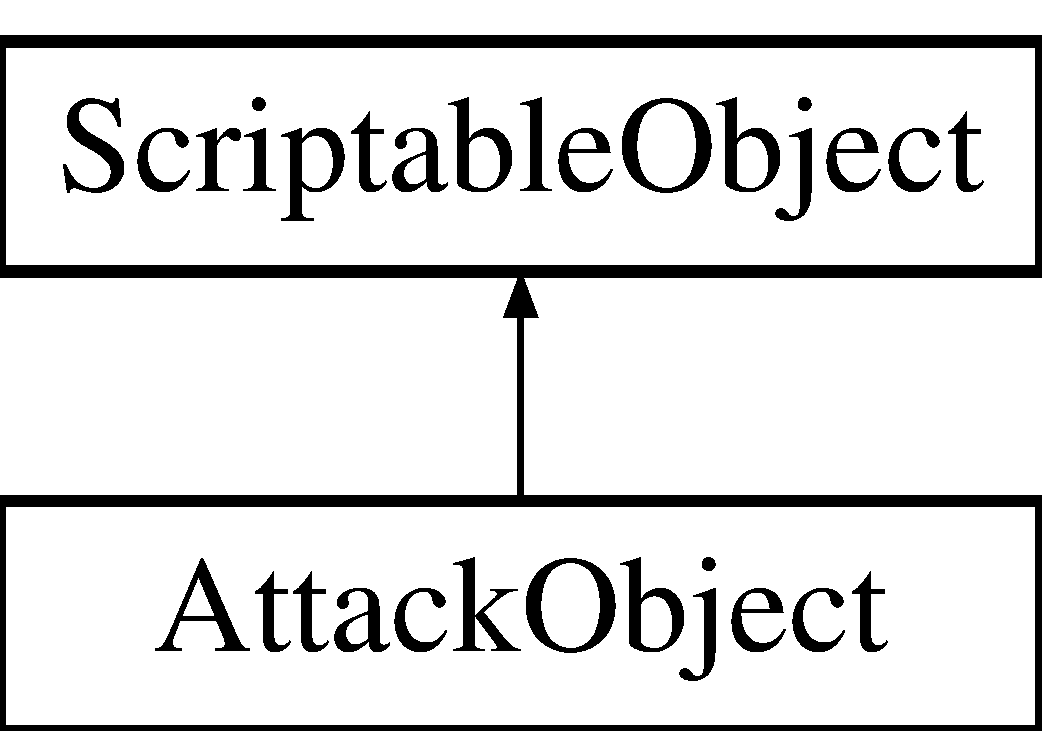
\includegraphics[height=2.000000cm]{class_attack_object}
\end{center}
\end{figure}
\subsection*{Public Member Functions}
\begin{DoxyCompactItemize}
\item 
\hypertarget{class_attack_object_a9d57cfc2f1cd8f3fac336e6eaa61de7b}{void {\bfseries Use\-Attack} ()}\label{class_attack_object_a9d57cfc2f1cd8f3fac336e6eaa61de7b}

\end{DoxyCompactItemize}
\subsection*{Public Attributes}
\begin{DoxyCompactItemize}
\item 
\hypertarget{class_attack_object_a77a64278632f48a1adf158f7942a1f6a}{string {\bfseries attack\-Name}}\label{class_attack_object_a77a64278632f48a1adf158f7942a1f6a}

\item 
\hypertarget{class_attack_object_acb154b106300b99626b300a864ae7feb}{Monster\-Type {\bfseries type}}\label{class_attack_object_acb154b106300b99626b300a864ae7feb}

\item 
\hypertarget{class_attack_object_a981d3937d15bd975788b897f024bab80}{Move\-Kind {\bfseries physical\-Or\-Special}}\label{class_attack_object_a981d3937d15bd975788b897f024bab80}

\item 
\hypertarget{class_attack_object_a928a00beb60b957f56b62591d8dfa2cf}{bool {\bfseries does\-Damage}}\label{class_attack_object_a928a00beb60b957f56b62591d8dfa2cf}

\item 
\hypertarget{class_attack_object_a45ebb18fe16c21ac71db0fb5c73c837d}{int {\bfseries power}}\label{class_attack_object_a45ebb18fe16c21ac71db0fb5c73c837d}

\item 
\hypertarget{class_attack_object_af1d7ec4f599e5a98aad5326b31c8abb6}{bool {\bfseries does\-Modifies\-Stats}}\label{class_attack_object_af1d7ec4f599e5a98aad5326b31c8abb6}

\item 
\hypertarget{class_attack_object_a0deab2293adc833a213fb64f264c45fd}{bool {\bfseries does\-Modify\-Opponent\-Stats}}\label{class_attack_object_a0deab2293adc833a213fb64f264c45fd}

\item 
\hypertarget{class_attack_object_aa573d5e02b9aeb3a114861e34fff686d}{int {\bfseries modify\-Attack\-Value}}\label{class_attack_object_aa573d5e02b9aeb3a114861e34fff686d}

\item 
\hypertarget{class_attack_object_a62a48ae9b1bc7a695a25612a0e2b8366}{int {\bfseries modify\-Defense\-Value}}\label{class_attack_object_a62a48ae9b1bc7a695a25612a0e2b8366}

\item 
\hypertarget{class_attack_object_a1ff22a96cca03518d05be97df2f8c691}{int {\bfseries modify\-Special\-Attack\-Value}}\label{class_attack_object_a1ff22a96cca03518d05be97df2f8c691}

\item 
\hypertarget{class_attack_object_a9c37f05dd050b329015be746fa69d650}{int {\bfseries modify\-Special\-Defense\-Value}}\label{class_attack_object_a9c37f05dd050b329015be746fa69d650}

\item 
\hypertarget{class_attack_object_abb0bed3e74f1afd7579bcc3b01097b21}{int {\bfseries modify\-Accuracy\-Value}}\label{class_attack_object_abb0bed3e74f1afd7579bcc3b01097b21}

\item 
\hypertarget{class_attack_object_a82f771a9ec05578c962a9570c4576efd}{int {\bfseries modify\-Speed\-Value}}\label{class_attack_object_a82f771a9ec05578c962a9570c4576efd}

\item 
\hypertarget{class_attack_object_a1950a855161b9b8e1070c355e909af97}{int {\bfseries accuracy}}\label{class_attack_object_a1950a855161b9b8e1070c355e909af97}

\item 
\hypertarget{class_attack_object_ae464864616e42f31c5b3a04bff282957}{int {\bfseries power\-Points}}\label{class_attack_object_ae464864616e42f31c5b3a04bff282957}

\end{DoxyCompactItemize}


The documentation for this class was generated from the following file\-:\begin{DoxyCompactItemize}
\item 
/home/travis/build/temportalflux/\-Champ\-Net/\-Unity/\-Assets/\-Scripts/\-Monster\-Scriptable\-Objects/Attack\-Object.\-cs\end{DoxyCompactItemize}

\hypertarget{class_attack_object_editor}{\section{Attack\-Object\-Editor Class Reference}
\label{class_attack_object_editor}\index{Attack\-Object\-Editor@{Attack\-Object\-Editor}}
}
Inheritance diagram for Attack\-Object\-Editor\-:\begin{figure}[H]
\begin{center}
\leavevmode
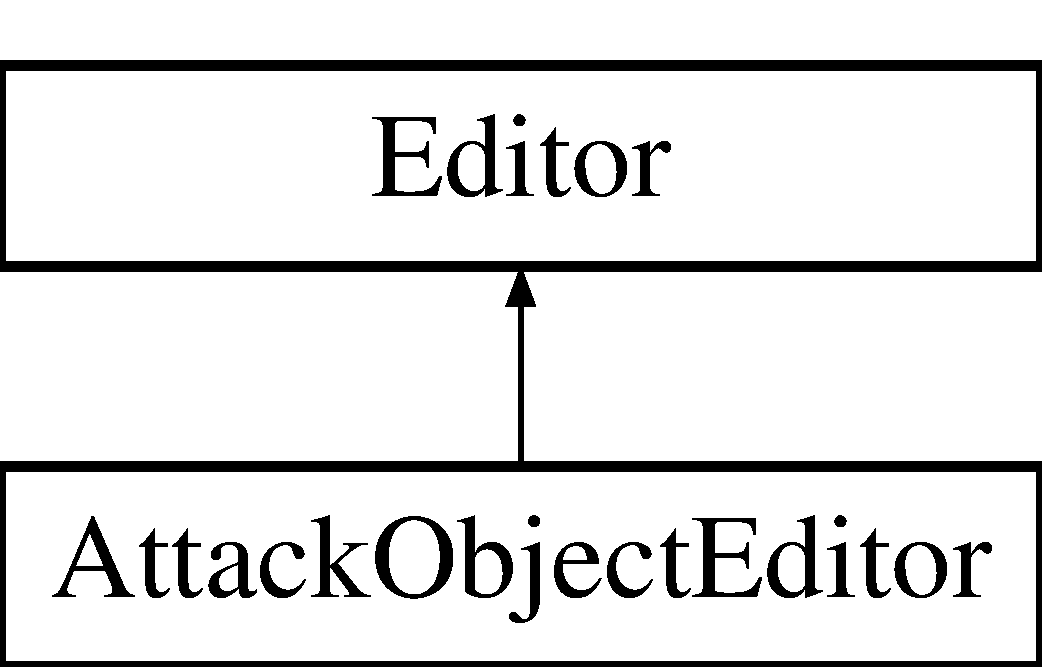
\includegraphics[height=2.000000cm]{class_attack_object_editor}
\end{center}
\end{figure}
\subsection*{Public Member Functions}
\begin{DoxyCompactItemize}
\item 
\hypertarget{class_attack_object_editor_ad41f5d42552191e05f82ba2f83afc673}{override void {\bfseries On\-Inspector\-G\-U\-I} ()}\label{class_attack_object_editor_ad41f5d42552191e05f82ba2f83afc673}

\end{DoxyCompactItemize}


The documentation for this class was generated from the following file\-:\begin{DoxyCompactItemize}
\item 
/home/travis/build/temportalflux/\-Champ\-Net/\-Unity/\-Assets/\-Scripts/\-Monster\-Scriptable\-Objects/\-Editor/Attack\-Object\-Editor.\-cs\end{DoxyCompactItemize}

\hypertarget{class_bit_serialize_attribute_1_1_attribute_field}{\section{Bit\-Serialize\-Attribute.\-Attribute\-Field Class Reference}
\label{class_bit_serialize_attribute_1_1_attribute_field}\index{Bit\-Serialize\-Attribute.\-Attribute\-Field@{Bit\-Serialize\-Attribute.\-Attribute\-Field}}
}
\subsection*{Public Attributes}
\begin{DoxyCompactItemize}
\item 
\hypertarget{class_bit_serialize_attribute_1_1_attribute_field_a5202edf5d3e0632b952595fba53f171b}{Field\-Info {\bfseries info} = null}\label{class_bit_serialize_attribute_1_1_attribute_field_a5202edf5d3e0632b952595fba53f171b}

\item 
\hypertarget{class_bit_serialize_attribute_1_1_attribute_field_a7ba4865ba3f2c1f6ee86966730861394}{int {\bfseries size} = 0}\label{class_bit_serialize_attribute_1_1_attribute_field_a7ba4865ba3f2c1f6ee86966730861394}

\item 
\hypertarget{class_bit_serialize_attribute_1_1_attribute_field_a5ca46d341ee4b04a261730b04004aa0e}{List$<$ \hyperlink{class_bit_serialize_attribute_1_1_attribute_field}{Attribute\-Field} $>$ {\bfseries fields} = new List$<$\hyperlink{class_bit_serialize_attribute_1_1_attribute_field}{Attribute\-Field}$>$()}\label{class_bit_serialize_attribute_1_1_attribute_field_a5ca46d341ee4b04a261730b04004aa0e}

\item 
\hypertarget{class_bit_serialize_attribute_1_1_attribute_field_a68e769f45a1b45e8a4d73102c1fae266}{List$<$ \hyperlink{class_bit_serialize_attribute_1_1_attribute_field}{Attribute\-Field} $>$ {\bfseries fieldsby\-Generic} = new List$<$\hyperlink{class_bit_serialize_attribute_1_1_attribute_field}{Attribute\-Field}$>$()}\label{class_bit_serialize_attribute_1_1_attribute_field_a68e769f45a1b45e8a4d73102c1fae266}

\end{DoxyCompactItemize}


The documentation for this class was generated from the following file\-:\begin{DoxyCompactItemize}
\item 
/home/travis/build/temportalflux/\-Champ\-Net/\-Unity/\-Assets/\-Scripts/\-Attribute/Bit\-Serialize\-Attribute.\-cs\end{DoxyCompactItemize}

\hypertarget{class_battle_handler}{\section{Battle\-Handler Class Reference}
\label{class_battle_handler}\index{Battle\-Handler@{Battle\-Handler}}
}


 


Inheritance diagram for Battle\-Handler\-:\begin{figure}[H]
\begin{center}
\leavevmode
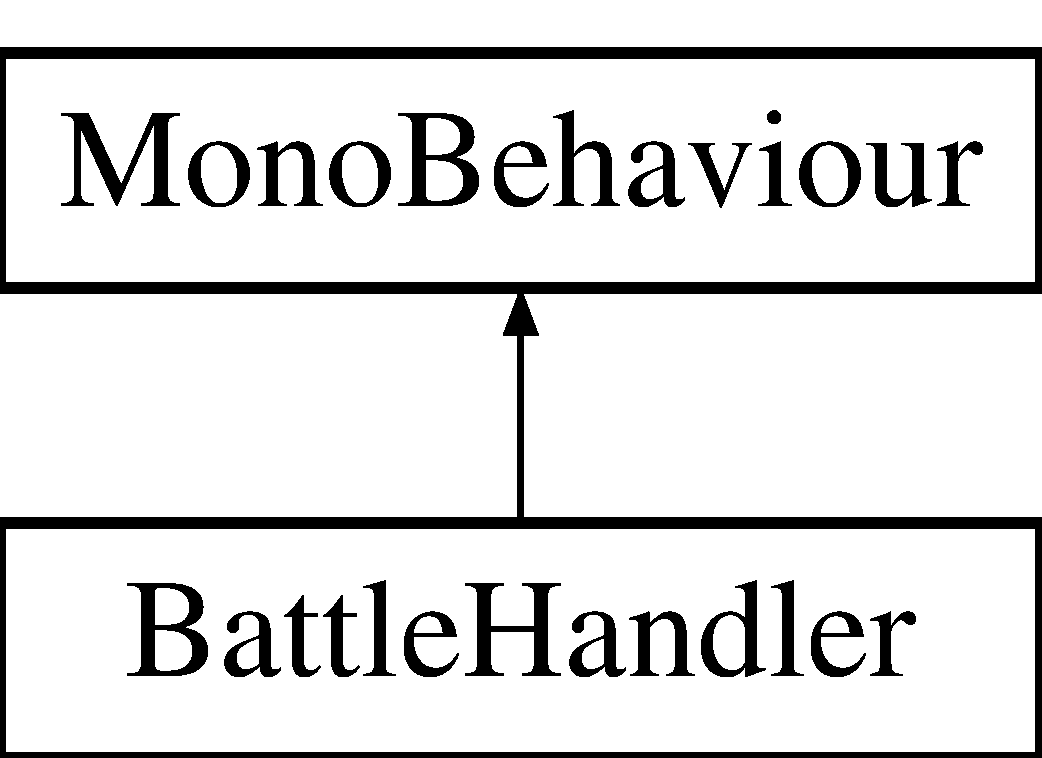
\includegraphics[height=2.000000cm]{class_battle_handler}
\end{center}
\end{figure}
\subsection*{Public Types}
\begin{DoxyCompactItemize}
\item 
enum {\bfseries Battle\-State} \{ {\bfseries W\-A\-I\-T\-I\-N\-G\-\_\-\-O\-N\-\_\-\-I\-N\-P\-U\-T}, 
{\bfseries D\-I\-S\-P\-L\-A\-Y\-I\-N\-G\-\_\-\-T\-U\-R\-N}
 \}
\end{DoxyCompactItemize}
\subsection*{Public Member Functions}
\begin{DoxyCompactItemize}
\item 
void \hyperlink{group__client_ga380a371e96df1b362027a8f33c8ed7fb}{Set\-Up\-Battle} (\hyperlink{class_battle_participant}{Battle\-Participant} first, \hyperlink{class_battle_participant}{Battle\-Participant} second, bool is\-Networked\-Battle)
\begin{DoxyCompactList}\small\item\em Called To set up the battle scene. Must be called at the start \end{DoxyCompactList}\item 
bool \hyperlink{group__client_gad207e2adf6f1f3882e98b1c8a5f59f67}{Send\-Battle\-Option} (bool is\-Local\-Player, \hyperlink{class_game_state_1_1_player_a9f54c5eca1e60acbaa2074e981f51615}{Game\-State.\-Player.\-Enum\-Battle\-Selection} selection, uint selection\-Index)
\begin{DoxyCompactList}\small\item\em Used to send a battle selection \end{DoxyCompactList}\item 
\hypertarget{group__client_gad69bfcfc81caec50b1db97edb95e33b1}{I\-Enumerator {\bfseries Handle\-Response} (\hyperlink{class_battle_participant}{Battle\-Participant} p1, \hyperlink{class_battle_participant}{Battle\-Participant} p2)}\label{group__client_gad69bfcfc81caec50b1db97edb95e33b1}

\item 
\hypertarget{group__client_ga13610e1414fd1f866292588574c96139}{void {\bfseries on\-Pre\-Exit} ()}\label{group__client_ga13610e1414fd1f866292588574c96139}

\end{DoxyCompactItemize}
\subsection*{Public Attributes}
\begin{DoxyCompactItemize}
\item 
\hypertarget{group__client_gad57da165c3aa4c3906b10dc80cca73e2}{\hyperlink{class_battle_u_i_controller}{Battle\-U\-I\-Controller} {\bfseries battle\-U\-I\-Controller}}\label{group__client_gad57da165c3aa4c3906b10dc80cca73e2}

\item 
bool \hyperlink{group__client_ga91faa80b5273370273762c40a364305d}{is\-Networked}
\begin{DoxyCompactList}\small\item\em Indicates that the current battle is between networked players \end{DoxyCompactList}\item 
\hypertarget{group__client_ga95fc9651e0a7845913c3a2bf1330e2cf}{\hyperlink{class_battle_participant}{Battle\-Participant} {\bfseries participant1}}\label{group__client_ga95fc9651e0a7845913c3a2bf1330e2cf}

\item 
\hypertarget{group__client_ga303ed561d4ed9408dfb02b03034ed2a9}{\hyperlink{class_battle_participant}{Battle\-Participant} {\bfseries participant2}}\label{group__client_ga303ed561d4ed9408dfb02b03034ed2a9}

\item 
readonly float\mbox{[}$\,$\mbox{]}\mbox{[}$\,$\mbox{]} {\bfseries type\-Match\-Up}
\end{DoxyCompactItemize}


\subsection{Detailed Description}


$<$author$>$Jake Ruth$<$/author$>$ 

The documentation for this class was generated from the following file\-:\begin{DoxyCompactItemize}
\item 
/home/travis/build/temportalflux/\-Champ\-Net/\-Unity/\-Assets/\-Scripts/\-Battles/Battle\-Handler.\-cs\end{DoxyCompactItemize}

\hypertarget{class_battle_participant}{\section{Battle\-Participant Class Reference}
\label{class_battle_participant}\index{Battle\-Participant@{Battle\-Participant}}
}


Class to hold information about a participant in a battle. Could be a local player, networked player, or cretin A\-I.  


\subsection*{Public Member Functions}
\begin{DoxyCompactItemize}
\item 
\hyperlink{class_battle_participant_aa08199f7a1456a22690a8a4b61da5089}{Battle\-Participant} (\hyperlink{class_game_state_1_1_player}{Game\-State.\-Player} player, int cretin)
\begin{DoxyCompactList}\small\item\em Instantiate the participant as a player, networked or local. \end{DoxyCompactList}\item 
\hyperlink{class_battle_participant_a636ea63e4b3f972767322e56aa5f3088}{Battle\-Participant} (\hyperlink{class_monster_data_object}{Monster\-Data\-Object} cretin\-A\-I)
\begin{DoxyCompactList}\small\item\em Instantiate the participant as a cretin A\-I. \end{DoxyCompactList}\item 
void \hyperlink{class_battle_participant_a32c2449a4bf42f88a7abd2ac5639add2}{swap\-Cretin\-To} (int index)
\begin{DoxyCompactList}\small\item\em Swaps the current cretin index for P\-L\-A\-Y\-E\-R participants. Performs fetch\-Current\-Cretin once the index is set. \end{DoxyCompactList}\item 
bool \hyperlink{class_battle_participant_a772329be78feaa3c85a692c39dc54a47}{is\-Player} ()
\begin{DoxyCompactList}\small\item\em Checks if the participant is a player. \end{DoxyCompactList}\end{DoxyCompactItemize}
\subsection*{Public Attributes}
\begin{DoxyCompactItemize}
\item 
\hyperlink{class_game_state_1_1_player}{Game\-State.\-Player} \hyperlink{class_battle_participant_a2f1584b2283c99eaaaa8e5b66ced968f}{player\-Controller}
\begin{DoxyCompactList}\small\item\em The Player info for the controlling player. Null if the controller is the opponent for a local player vs A\-I battle. \end{DoxyCompactList}\item 
\hyperlink{class_monster_data_object}{Monster\-Data\-Object} \hyperlink{class_battle_participant_a595abdc8d0d62918b99b37ea9d948d00}{current\-Cretin}
\begin{DoxyCompactList}\small\item\em The current cretin in battle. If \hyperlink{class_battle_participant_a2f1584b2283c99eaaaa8e5b66ced968f}{player\-Controller} is non-\/null, \hyperlink{class_battle_participant_a595abdc8d0d62918b99b37ea9d948d00}{current\-Cretin} = \end{DoxyCompactList}\item 
int \hyperlink{class_battle_participant_a1ad2e6be9469ff3c433be70fc6245484}{current\-Cretin\-Index}
\begin{DoxyCompactList}\small\item\em The current index of the cretin in the controller. -\/1 if the controller is the opponent for a local player vs A\-I battle. \end{DoxyCompactList}\item 
\hyperlink{class_game_state_1_1_player_a9f54c5eca1e60acbaa2074e981f51615}{Game\-State.\-Player.\-Enum\-Battle\-Selection} \hyperlink{class_battle_participant_abf036cb064ddcd97270c1b9ed8442f50}{selection}
\begin{DoxyCompactList}\small\item\em The latest selection of the player/\-A\-I. \end{DoxyCompactList}\item 
int \hyperlink{class_battle_participant_a30032b373a898bbb16f67e24bf245557}{selection\-Choice} = -\/1
\begin{DoxyCompactList}\small\item\em The latest selection choice of the player/\-A\-I. \end{DoxyCompactList}\end{DoxyCompactItemize}


\subsection{Detailed Description}
Class to hold information about a participant in a battle. Could be a local player, networked player, or cretin A\-I. 



\subsection{Constructor \& Destructor Documentation}
\hypertarget{class_battle_participant_aa08199f7a1456a22690a8a4b61da5089}{\index{Battle\-Participant@{Battle\-Participant}!Battle\-Participant@{Battle\-Participant}}
\index{Battle\-Participant@{Battle\-Participant}!BattleParticipant@{Battle\-Participant}}
\subsubsection[{Battle\-Participant}]{\setlength{\rightskip}{0pt plus 5cm}Battle\-Participant.\-Battle\-Participant (
\begin{DoxyParamCaption}
\item[{{\bf Game\-State.\-Player}}]{player, }
\item[{int}]{cretin}
\end{DoxyParamCaption}
)\hspace{0.3cm}{\ttfamily [inline]}}}\label{class_battle_participant_aa08199f7a1456a22690a8a4b61da5089}


Instantiate the participant as a player, networked or local. 


\begin{DoxyParams}{Parameters}
{\em player} & The player state.\\
\hline
{\em cretin} & The cretin index in {\ttfamily \hyperlink{class_game_state_1_1_player}{Game\-State.\-Player}.monsters}\\
\hline
\end{DoxyParams}
\hypertarget{class_battle_participant_a636ea63e4b3f972767322e56aa5f3088}{\index{Battle\-Participant@{Battle\-Participant}!Battle\-Participant@{Battle\-Participant}}
\index{Battle\-Participant@{Battle\-Participant}!BattleParticipant@{Battle\-Participant}}
\subsubsection[{Battle\-Participant}]{\setlength{\rightskip}{0pt plus 5cm}Battle\-Participant.\-Battle\-Participant (
\begin{DoxyParamCaption}
\item[{{\bf Monster\-Data\-Object}}]{cretin\-A\-I}
\end{DoxyParamCaption}
)\hspace{0.3cm}{\ttfamily [inline]}}}\label{class_battle_participant_a636ea63e4b3f972767322e56aa5f3088}


Instantiate the participant as a cretin A\-I. 


\begin{DoxyParams}{Parameters}
{\em cretin\-A\-I} & The monster stats for the battling cretin.\\
\hline
\end{DoxyParams}


\subsection{Member Function Documentation}
\hypertarget{class_battle_participant_a772329be78feaa3c85a692c39dc54a47}{\index{Battle\-Participant@{Battle\-Participant}!is\-Player@{is\-Player}}
\index{is\-Player@{is\-Player}!BattleParticipant@{Battle\-Participant}}
\subsubsection[{is\-Player}]{\setlength{\rightskip}{0pt plus 5cm}bool Battle\-Participant.\-is\-Player (
\begin{DoxyParamCaption}
{}
\end{DoxyParamCaption}
)\hspace{0.3cm}{\ttfamily [inline]}}}\label{class_battle_participant_a772329be78feaa3c85a692c39dc54a47}


Checks if the participant is a player. 

\begin{DoxyReturn}{Returns}
{\ttfamily True}, if \hyperlink{class_battle_participant_a2f1584b2283c99eaaaa8e5b66ced968f}{player\-Controller} is non-\/null.
\end{DoxyReturn}
\hypertarget{class_battle_participant_a32c2449a4bf42f88a7abd2ac5639add2}{\index{Battle\-Participant@{Battle\-Participant}!swap\-Cretin\-To@{swap\-Cretin\-To}}
\index{swap\-Cretin\-To@{swap\-Cretin\-To}!BattleParticipant@{Battle\-Participant}}
\subsubsection[{swap\-Cretin\-To}]{\setlength{\rightskip}{0pt plus 5cm}void Battle\-Participant.\-swap\-Cretin\-To (
\begin{DoxyParamCaption}
\item[{int}]{index}
\end{DoxyParamCaption}
)\hspace{0.3cm}{\ttfamily [inline]}}}\label{class_battle_participant_a32c2449a4bf42f88a7abd2ac5639add2}


Swaps the current cretin index for P\-L\-A\-Y\-E\-R participants. Performs fetch\-Current\-Cretin once the index is set. 


\begin{DoxyParams}{Parameters}
{\em index} & The new index for the cretin.\\
\hline
\end{DoxyParams}


\subsection{Member Data Documentation}
\hypertarget{class_battle_participant_a595abdc8d0d62918b99b37ea9d948d00}{\index{Battle\-Participant@{Battle\-Participant}!current\-Cretin@{current\-Cretin}}
\index{current\-Cretin@{current\-Cretin}!BattleParticipant@{Battle\-Participant}}
\subsubsection[{current\-Cretin}]{\setlength{\rightskip}{0pt plus 5cm}{\bf Monster\-Data\-Object} Battle\-Participant.\-current\-Cretin}}\label{class_battle_participant_a595abdc8d0d62918b99b37ea9d948d00}


The current cretin in battle. If \hyperlink{class_battle_participant_a2f1584b2283c99eaaaa8e5b66ced968f}{player\-Controller} is non-\/null, \hyperlink{class_battle_participant_a595abdc8d0d62918b99b37ea9d948d00}{current\-Cretin} = 

{\ttfamily \hyperlink{class_battle_participant_a2f1584b2283c99eaaaa8e5b66ced968f}{player\-Controller}.monsters\mbox{[}\hyperlink{class_battle_participant_a1ad2e6be9469ff3c433be70fc6245484}{current\-Cretin\-Index}\mbox{]}}. \hypertarget{class_battle_participant_a1ad2e6be9469ff3c433be70fc6245484}{\index{Battle\-Participant@{Battle\-Participant}!current\-Cretin\-Index@{current\-Cretin\-Index}}
\index{current\-Cretin\-Index@{current\-Cretin\-Index}!BattleParticipant@{Battle\-Participant}}
\subsubsection[{current\-Cretin\-Index}]{\setlength{\rightskip}{0pt plus 5cm}int Battle\-Participant.\-current\-Cretin\-Index}}\label{class_battle_participant_a1ad2e6be9469ff3c433be70fc6245484}


The current index of the cretin in the controller. -\/1 if the controller is the opponent for a local player vs A\-I battle. 

\hypertarget{class_battle_participant_a2f1584b2283c99eaaaa8e5b66ced968f}{\index{Battle\-Participant@{Battle\-Participant}!player\-Controller@{player\-Controller}}
\index{player\-Controller@{player\-Controller}!BattleParticipant@{Battle\-Participant}}
\subsubsection[{player\-Controller}]{\setlength{\rightskip}{0pt plus 5cm}{\bf Game\-State.\-Player} Battle\-Participant.\-player\-Controller}}\label{class_battle_participant_a2f1584b2283c99eaaaa8e5b66ced968f}


The Player info for the controlling player. Null if the controller is the opponent for a local player vs A\-I battle. 

\hypertarget{class_battle_participant_abf036cb064ddcd97270c1b9ed8442f50}{\index{Battle\-Participant@{Battle\-Participant}!selection@{selection}}
\index{selection@{selection}!BattleParticipant@{Battle\-Participant}}
\subsubsection[{selection}]{\setlength{\rightskip}{0pt plus 5cm}{\bf Game\-State.\-Player.\-Enum\-Battle\-Selection} Battle\-Participant.\-selection}}\label{class_battle_participant_abf036cb064ddcd97270c1b9ed8442f50}


The latest selection of the player/\-A\-I. 

\hypertarget{class_battle_participant_a30032b373a898bbb16f67e24bf245557}{\index{Battle\-Participant@{Battle\-Participant}!selection\-Choice@{selection\-Choice}}
\index{selection\-Choice@{selection\-Choice}!BattleParticipant@{Battle\-Participant}}
\subsubsection[{selection\-Choice}]{\setlength{\rightskip}{0pt plus 5cm}int Battle\-Participant.\-selection\-Choice = -\/1}}\label{class_battle_participant_a30032b373a898bbb16f67e24bf245557}


The latest selection choice of the player/\-A\-I. 



The documentation for this class was generated from the following file\-:\begin{DoxyCompactItemize}
\item 
/home/travis/build/temportalflux/\-Champ\-Net/\-Unity/\-Assets/\-Scripts/\-Battles/Battle\-Participant.\-cs\end{DoxyCompactItemize}

\hypertarget{class_battle_tester}{\section{Battle\-Tester Class Reference}
\label{class_battle_tester}\index{Battle\-Tester@{Battle\-Tester}}
}
Inheritance diagram for Battle\-Tester\-:\begin{figure}[H]
\begin{center}
\leavevmode
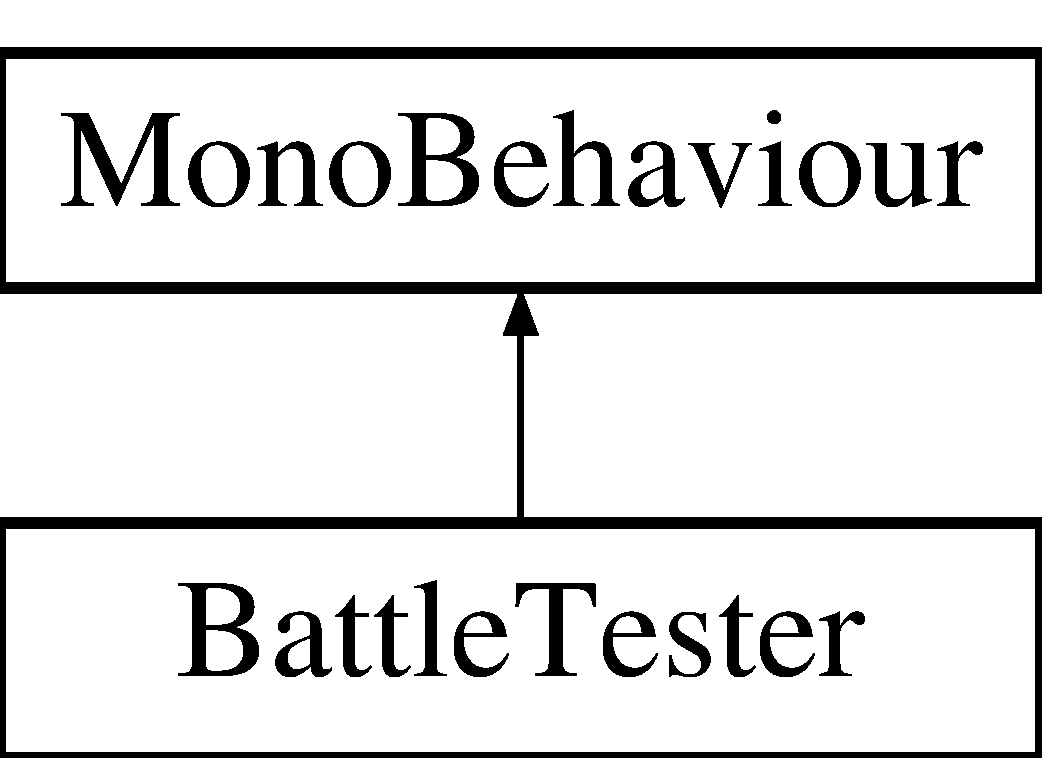
\includegraphics[height=2.000000cm]{class_battle_tester}
\end{center}
\end{figure}
\subsection*{Public Attributes}
\begin{DoxyCompactItemize}
\item 
\hypertarget{class_battle_tester_a87c03ddd5b47eb2881580fa62588660f}{\hyperlink{class_battle_handler}{Battle\-Handler} {\bfseries battle\-Handler}}\label{class_battle_tester_a87c03ddd5b47eb2881580fa62588660f}

\item 
\hypertarget{class_battle_tester_ab0a3a610e839111f2a5d460c9c140a1f}{\hyperlink{class_battle_u_i_controller}{Battle\-U\-I\-Controller} {\bfseries battle\-U\-I\-Controller}}\label{class_battle_tester_ab0a3a610e839111f2a5d460c9c140a1f}

\item 
\hypertarget{class_battle_tester_ad602b424310978effe2bed83ff7e9571}{\hyperlink{class_battle_participant}{Battle\-Participant} {\bfseries local\-Player\-Test}}\label{class_battle_tester_ad602b424310978effe2bed83ff7e9571}

\item 
\hypertarget{class_battle_tester_a9667e7e35242d772a7089a27027da3c0}{\hyperlink{class_battle_participant}{Battle\-Participant} {\bfseries other\-Player\-Test}}\label{class_battle_tester_a9667e7e35242d772a7089a27027da3c0}

\item 
\hypertarget{class_battle_tester_addc9371e367be0ad46f15d4e4556d632}{\hyperlink{class_monster_data_object}{Monster\-Data\-Object} {\bfseries monster\-A}}\label{class_battle_tester_addc9371e367be0ad46f15d4e4556d632}

\item 
\hypertarget{class_battle_tester_a558e144bf03fac9c26f3d4f4aaaf7c85}{\hyperlink{class_monster_data_object}{Monster\-Data\-Object} {\bfseries monster\-B}}\label{class_battle_tester_a558e144bf03fac9c26f3d4f4aaaf7c85}

\end{DoxyCompactItemize}
\subsection*{Protected Attributes}
\begin{DoxyCompactItemize}
\item 
\hypertarget{class_battle_tester_a39cd5d1c4a86ae22eb25d9a6d6674db9}{bool {\bfseries is\-Battle\-Setup}}\label{class_battle_tester_a39cd5d1c4a86ae22eb25d9a6d6674db9}

\end{DoxyCompactItemize}
\subsection*{Properties}
\begin{DoxyCompactItemize}
\item 
\hypertarget{class_battle_tester_afb877324567ebd5ac0d4f5372006d0fa}{bool {\bfseries Is\-Battle\-Setup}\hspace{0.3cm}{\ttfamily  \mbox{[}get, set\mbox{]}}}\label{class_battle_tester_afb877324567ebd5ac0d4f5372006d0fa}

\end{DoxyCompactItemize}


The documentation for this class was generated from the following file\-:\begin{DoxyCompactItemize}
\item 
/home/travis/build/temportalflux/\-Champ\-Net/\-Unity/\-Assets/\-Scripts/\-Battles/Battle\-Tester.\-cs\end{DoxyCompactItemize}

\hypertarget{class_battle_tester_editor}{\section{Battle\-Tester\-Editor Class Reference}
\label{class_battle_tester_editor}\index{Battle\-Tester\-Editor@{Battle\-Tester\-Editor}}
}
Inheritance diagram for Battle\-Tester\-Editor\-:\begin{figure}[H]
\begin{center}
\leavevmode
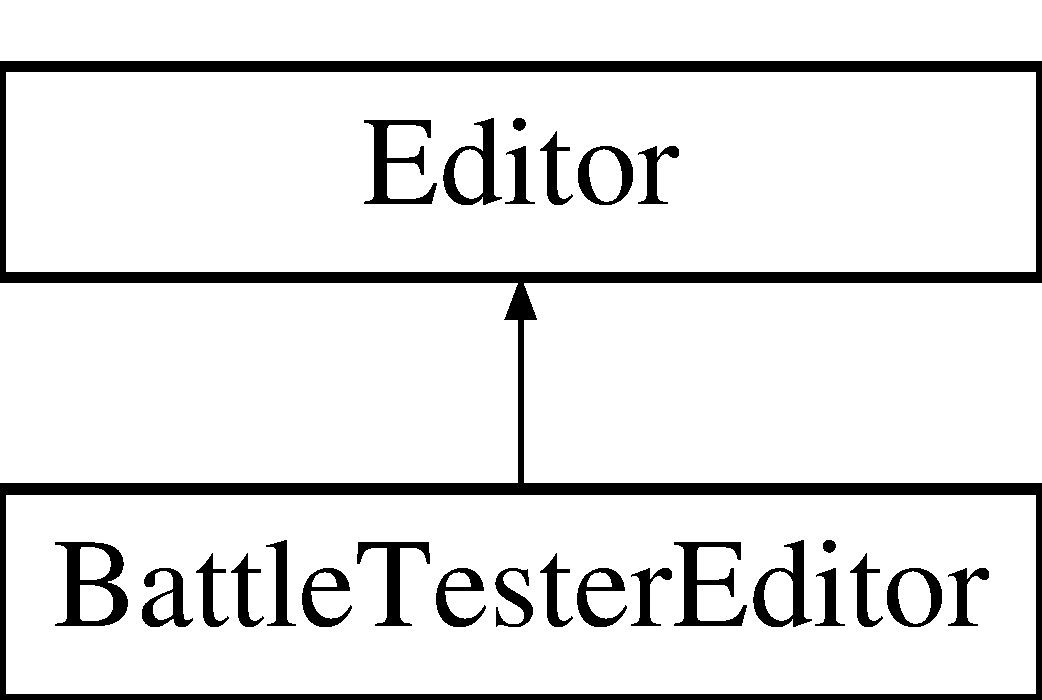
\includegraphics[height=2.000000cm]{class_battle_tester_editor}
\end{center}
\end{figure}
\subsection*{Public Member Functions}
\begin{DoxyCompactItemize}
\item 
\hypertarget{class_battle_tester_editor_a8826a03758478f108e1241f0c33f3658}{override void {\bfseries On\-Inspector\-G\-U\-I} ()}\label{class_battle_tester_editor_a8826a03758478f108e1241f0c33f3658}

\end{DoxyCompactItemize}


The documentation for this class was generated from the following file\-:\begin{DoxyCompactItemize}
\item 
/home/travis/build/temportalflux/\-Champ\-Net/\-Unity/\-Assets/\-Scripts/\-Battles/\-Editor/Battle\-Tester\-Editor.\-cs\end{DoxyCompactItemize}

\hypertarget{class_battle_u_i_controller}{\section{Battle\-U\-I\-Controller Class Reference}
\label{class_battle_u_i_controller}\index{Battle\-U\-I\-Controller@{Battle\-U\-I\-Controller}}
}
Inheritance diagram for Battle\-U\-I\-Controller\-:\begin{figure}[H]
\begin{center}
\leavevmode
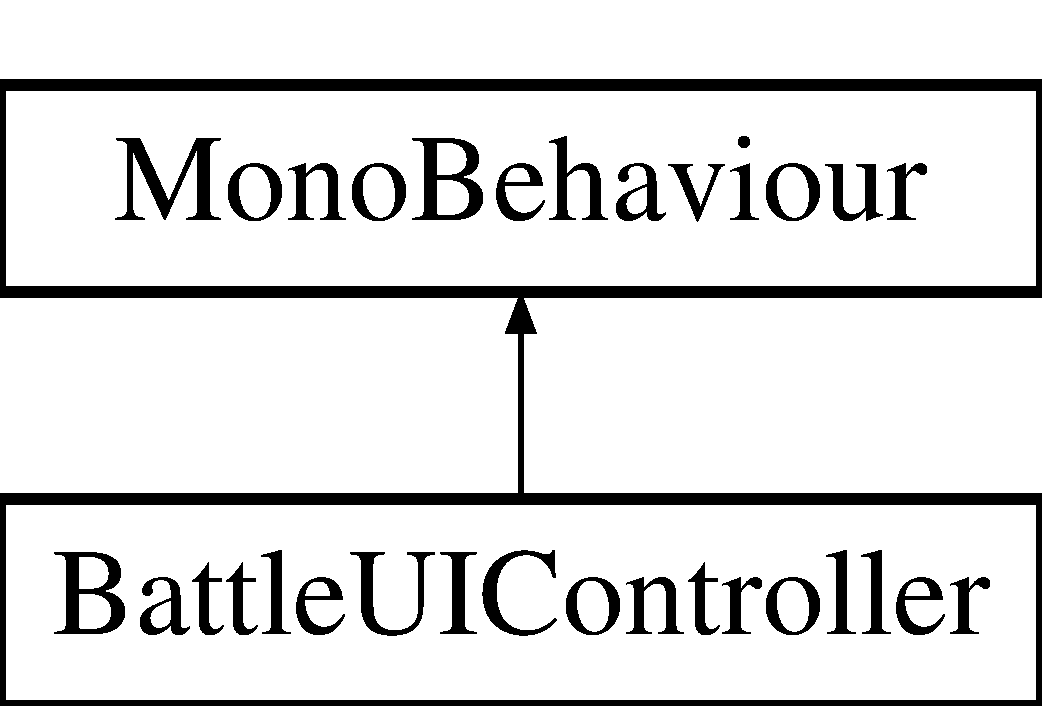
\includegraphics[height=2.000000cm]{class_battle_u_i_controller}
\end{center}
\end{figure}
\subsection*{Public Member Functions}
\begin{DoxyCompactItemize}
\item 
\hypertarget{class_battle_u_i_controller_a8c7cc90f2e90565d988a61531005504d}{void {\bfseries Button\-Clicked} (uint button\-Index)}\label{class_battle_u_i_controller_a8c7cc90f2e90565d988a61531005504d}

\item 
\hypertarget{class_battle_u_i_controller_a7cdd677370faa1526e0774b2b070e6fd}{void {\bfseries Back\-Button\-Clicked} ()}\label{class_battle_u_i_controller_a7cdd677370faa1526e0774b2b070e6fd}

\item 
\hypertarget{class_battle_u_i_controller_a05427e5dab5da5027fd3f12526e7d98c}{void {\bfseries Set\-Flavor\-Text} (string text)}\label{class_battle_u_i_controller_a05427e5dab5da5027fd3f12526e7d98c}

\end{DoxyCompactItemize}
\subsection*{Public Attributes}
\begin{DoxyCompactItemize}
\item 
\hypertarget{class_battle_u_i_controller_a1b3ecd57ac7d9161ea56b8942003a2b5}{\hyperlink{class_battle_handler}{Battle\-Handler} {\bfseries battle\-Handler}}\label{class_battle_u_i_controller_a1b3ecd57ac7d9161ea56b8942003a2b5}

\item 
\hypertarget{class_battle_u_i_controller_ab272bc3fa2feae7a46ee866a5252d47b}{Game\-Object {\bfseries main\-Menu\-Game\-Object}}\label{class_battle_u_i_controller_ab272bc3fa2feae7a46ee866a5252d47b}

\item 
\hypertarget{class_battle_u_i_controller_a0c493074ee8edeaaeafd6be0792f1b8e}{Game\-Object {\bfseries attack\-Menu\-Game\-Object}}\label{class_battle_u_i_controller_a0c493074ee8edeaaeafd6be0792f1b8e}

\item 
\hypertarget{class_battle_u_i_controller_af99e8408c55ed31be12051692750cb97}{Game\-Object {\bfseries items\-Menu\-Game\-Object}}\label{class_battle_u_i_controller_af99e8408c55ed31be12051692750cb97}

\item 
\hypertarget{class_battle_u_i_controller_a980ceadc6a8df5e2993b6fc97dc89083}{Game\-Object {\bfseries switch\-Menu\-Game\-Object}}\label{class_battle_u_i_controller_a980ceadc6a8df5e2993b6fc97dc89083}

\item 
\hypertarget{class_battle_u_i_controller_af29f6bee62095208f55a9d3fee5a628c}{Game\-Object {\bfseries forfeit\-Menu\-Game\-Object}}\label{class_battle_u_i_controller_af29f6bee62095208f55a9d3fee5a628c}

\item 
\hypertarget{class_battle_u_i_controller_ad6f40ffcec5911934218836218995e41}{Game\-Object {\bfseries waiting\-Game\-Object}}\label{class_battle_u_i_controller_ad6f40ffcec5911934218836218995e41}

\item 
\hypertarget{class_battle_u_i_controller_a57dc6e1b53d2412dd00eb29859bac337}{Button\mbox{[}$\,$\mbox{]} {\bfseries attack\-Buttons}}\label{class_battle_u_i_controller_a57dc6e1b53d2412dd00eb29859bac337}

\item 
\hypertarget{class_battle_u_i_controller_a188d6c1d20ceab7503469b77818cb7fc}{Button\mbox{[}$\,$\mbox{]} {\bfseries cretin\-Buttons}}\label{class_battle_u_i_controller_a188d6c1d20ceab7503469b77818cb7fc}

\item 
\hypertarget{class_battle_u_i_controller_a2f5cb0c646d3675c7c7805381d7e54d2}{Text {\bfseries waiting\-Text}}\label{class_battle_u_i_controller_a2f5cb0c646d3675c7c7805381d7e54d2}

\end{DoxyCompactItemize}
\subsection*{Properties}
\begin{DoxyCompactItemize}
\item 
\hypertarget{class_battle_u_i_controller_a4f8584c7f4ebdeb9b29bf982dc8a5e5d}{Menu\-State {\bfseries menu\-State}\hspace{0.3cm}{\ttfamily  \mbox{[}get, set\mbox{]}}}\label{class_battle_u_i_controller_a4f8584c7f4ebdeb9b29bf982dc8a5e5d}

\end{DoxyCompactItemize}


The documentation for this class was generated from the following file\-:\begin{DoxyCompactItemize}
\item 
/home/travis/build/temportalflux/\-Champ\-Net/\-Unity/\-Assets/\-Scripts/\-Battles/Battle\-U\-I\-Controller.\-cs\end{DoxyCompactItemize}

\hypertarget{class_bit_serialize_attribute}{\section{Bit\-Serialize\-Attribute Class Reference}
\label{class_bit_serialize_attribute}\index{Bit\-Serialize\-Attribute@{Bit\-Serialize\-Attribute}}
}


Handles (de)serializing of specific fields. Valid types include\-: bool, byte, char, (u)short, (u)int, (u)long, float, double, \hyperlink{interface_i_serializing}{I\-Serializing}, and any composite arrays of the former. If the Mono\-Behaviour being serialized is \hyperlink{interface_i_serializing}{I\-Serializing}, the \hyperlink{interface_i_serializing}{I\-Serializing} methods are treated as additions to all fields marked with Bit\-Serialize  


Inheritance diagram for Bit\-Serialize\-Attribute\-:\begin{figure}[H]
\begin{center}
\leavevmode
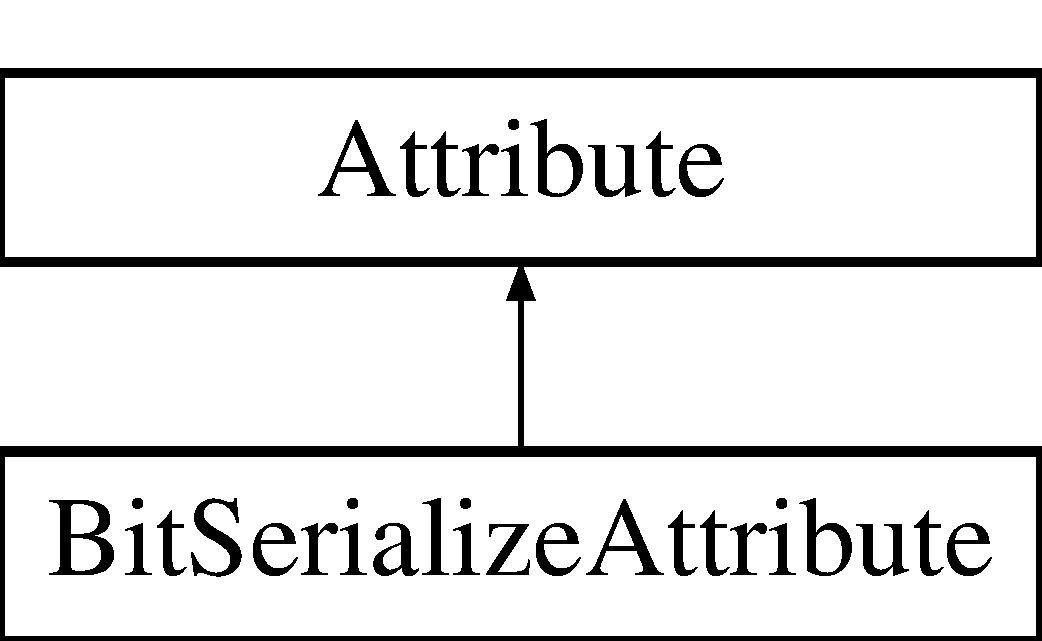
\includegraphics[height=2.000000cm]{class_bit_serialize_attribute}
\end{center}
\end{figure}
\subsection*{Static Public Member Functions}
\begin{DoxyCompactItemize}
\item 
static byte\mbox{[}$\,$\mbox{]} \hyperlink{class_bit_serialize_attribute_a0d934db4b1bdd25dbb3ef5ba6536f6c3}{Serialize$<$ T $>$} (T mono)
\begin{DoxyCompactList}\small\item\em Serialize a monobehavior to a byte array, using Bit\-Serialize and \hyperlink{interface_i_serializing}{I\-Serializing} \end{DoxyCompactList}\item 
static int \hyperlink{class_bit_serialize_attribute_a45dcbeb6ab33c11f4d6cc4971bb4ba55}{Get\-Size\-Of} (object value)
\begin{DoxyCompactList}\small\item\em Attempts to determine the size of some object (effectively sizeof(object)) \end{DoxyCompactList}\item 
static void \hyperlink{class_bit_serialize_attribute_aca1cc7a1f81cfffcf0ae04058d2da2c9}{Copy\-To} (ref byte\mbox{[}$\,$\mbox{]} dest, ref int offset, byte\mbox{[}$\,$\mbox{]} source)
\begin{DoxyCompactList}\small\item\em Write some byte array into another byte array at some offset \end{DoxyCompactList}\item 
static void \hyperlink{class_bit_serialize_attribute_ae92d448c6f7bf6ffab890747e1737c65}{Deserialize$<$ T $>$} (T mono, byte\mbox{[}$\,$\mbox{]} data)
\begin{DoxyCompactList}\small\item\em Deserialize a byte array into a monobehavior \end{DoxyCompactList}\end{DoxyCompactItemize}


\subsection{Detailed Description}
Handles (de)serializing of specific fields. Valid types include\-: bool, byte, char, (u)short, (u)int, (u)long, float, double, \hyperlink{interface_i_serializing}{I\-Serializing}, and any composite arrays of the former. If the Mono\-Behaviour being serialized is \hyperlink{interface_i_serializing}{I\-Serializing}, the \hyperlink{interface_i_serializing}{I\-Serializing} methods are treated as additions to all fields marked with Bit\-Serialize 



\subsection{Member Function Documentation}
\hypertarget{class_bit_serialize_attribute_aca1cc7a1f81cfffcf0ae04058d2da2c9}{\index{Bit\-Serialize\-Attribute@{Bit\-Serialize\-Attribute}!Copy\-To@{Copy\-To}}
\index{Copy\-To@{Copy\-To}!BitSerializeAttribute@{Bit\-Serialize\-Attribute}}
\subsubsection[{Copy\-To}]{\setlength{\rightskip}{0pt plus 5cm}static void Bit\-Serialize\-Attribute.\-Copy\-To (
\begin{DoxyParamCaption}
\item[{ref byte\mbox{[}$\,$\mbox{]}}]{dest, }
\item[{ref int}]{offset, }
\item[{byte\mbox{[}$\,$\mbox{]}}]{source}
\end{DoxyParamCaption}
)\hspace{0.3cm}{\ttfamily [inline]}, {\ttfamily [static]}}}\label{class_bit_serialize_attribute_aca1cc7a1f81cfffcf0ae04058d2da2c9}


Write some byte array into another byte array at some offset 


\begin{DoxyParams}{Parameters}
{\em dest} & The data to copy.\\
\hline
{\em offset} & The offset in bytes.\\
\hline
{\em source} & The data object to copy into at the offset.\\
\hline
\end{DoxyParams}


Author\-: Dustin Yost \hypertarget{class_bit_serialize_attribute_ae92d448c6f7bf6ffab890747e1737c65}{\index{Bit\-Serialize\-Attribute@{Bit\-Serialize\-Attribute}!Deserialize$<$ T $>$@{Deserialize$<$ T $>$}}
\index{Deserialize$<$ T $>$@{Deserialize$<$ T $>$}!BitSerializeAttribute@{Bit\-Serialize\-Attribute}}
\subsubsection[{Deserialize$<$ T $>$}]{\setlength{\rightskip}{0pt plus 5cm}static void Bit\-Serialize\-Attribute.\-Deserialize$<$ T $>$ (
\begin{DoxyParamCaption}
\item[{T}]{mono, }
\item[{byte\mbox{[}$\,$\mbox{]}}]{data}
\end{DoxyParamCaption}
)\hspace{0.3cm}{\ttfamily [inline]}, {\ttfamily [static]}}}\label{class_bit_serialize_attribute_ae92d448c6f7bf6ffab890747e1737c65}


Deserialize a byte array into a monobehavior 


\begin{DoxyParams}{Parameters}
{\em mono} & The monobehavior to set data in\\
\hline
{\em data} & A byte array of data created with Serialize\\
\hline
\end{DoxyParams}
\hypertarget{class_bit_serialize_attribute_a45dcbeb6ab33c11f4d6cc4971bb4ba55}{\index{Bit\-Serialize\-Attribute@{Bit\-Serialize\-Attribute}!Get\-Size\-Of@{Get\-Size\-Of}}
\index{Get\-Size\-Of@{Get\-Size\-Of}!BitSerializeAttribute@{Bit\-Serialize\-Attribute}}
\subsubsection[{Get\-Size\-Of}]{\setlength{\rightskip}{0pt plus 5cm}static int Bit\-Serialize\-Attribute.\-Get\-Size\-Of (
\begin{DoxyParamCaption}
\item[{object}]{value}
\end{DoxyParamCaption}
)\hspace{0.3cm}{\ttfamily [inline]}, {\ttfamily [static]}}}\label{class_bit_serialize_attribute_a45dcbeb6ab33c11f4d6cc4971bb4ba55}


Attempts to determine the size of some object (effectively sizeof(object)) 


\begin{DoxyParams}{Parameters}
{\em value} & The object to size up\\
\hline
\end{DoxyParams}
\begin{DoxyReturn}{Returns}
The size of some object, using sizeof for primitive objects, recursive behavior for arrays, and Get\-Size for \hyperlink{interface_i_serializing}{I\-Serializing}
\end{DoxyReturn}
\hypertarget{class_bit_serialize_attribute_a0d934db4b1bdd25dbb3ef5ba6536f6c3}{\index{Bit\-Serialize\-Attribute@{Bit\-Serialize\-Attribute}!Serialize$<$ T $>$@{Serialize$<$ T $>$}}
\index{Serialize$<$ T $>$@{Serialize$<$ T $>$}!BitSerializeAttribute@{Bit\-Serialize\-Attribute}}
\subsubsection[{Serialize$<$ T $>$}]{\setlength{\rightskip}{0pt plus 5cm}static byte \mbox{[}$\,$\mbox{]} Bit\-Serialize\-Attribute.\-Serialize$<$ T $>$ (
\begin{DoxyParamCaption}
\item[{T}]{mono}
\end{DoxyParamCaption}
)\hspace{0.3cm}{\ttfamily [inline]}, {\ttfamily [static]}}}\label{class_bit_serialize_attribute_a0d934db4b1bdd25dbb3ef5ba6536f6c3}


Serialize a monobehavior to a byte array, using Bit\-Serialize and \hyperlink{interface_i_serializing}{I\-Serializing} 


\begin{DoxyParams}{Parameters}
{\em mono} & The monobehavior to serialize\\
\hline
\end{DoxyParams}
\begin{DoxyReturn}{Returns}
A byte array of data formatted in the order of fields and extra data according to \hyperlink{interface_i_serializing}{I\-Serializing}
\end{DoxyReturn}


The documentation for this class was generated from the following file\-:\begin{DoxyCompactItemize}
\item 
/home/travis/build/temportalflux/\-Champ\-Net/\-Unity/\-Assets/\-Scripts/\-Attribute/Bit\-Serialize\-Attribute.\-cs\end{DoxyCompactItemize}

\hypertarget{class_bit_serializing}{\section{Bit\-Serializing Class Reference}
\label{class_bit_serializing}\index{Bit\-Serializing@{Bit\-Serializing}}
}


\subsection{Detailed Description}
\begin{DoxyAuthor}{Author}
Dustin Yost 
\end{DoxyAuthor}


The documentation for this class was generated from the following file\-:\begin{DoxyCompactItemize}
\item 
/home/travis/build/temportalflux/\-Champ\-Net/\-Unity/\-Assets/\-Scripts/Bit\-Serializing.\-cs\end{DoxyCompactItemize}

\hypertarget{class_bit_test}{\section{Bit\-Test Class Reference}
\label{class_bit_test}\index{Bit\-Test@{Bit\-Test}}
}
Inheritance diagram for Bit\-Test\-:\begin{figure}[H]
\begin{center}
\leavevmode
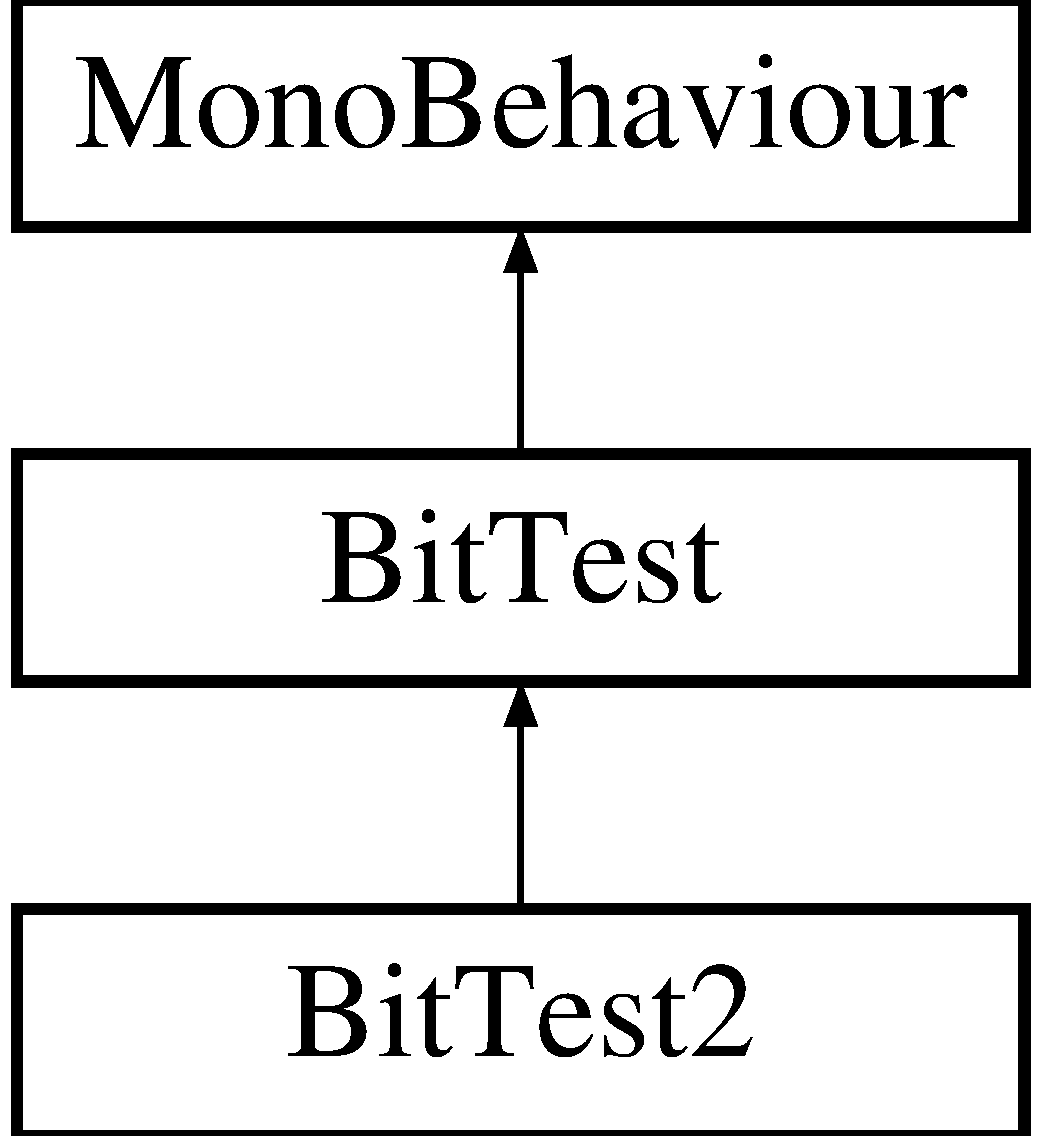
\includegraphics[height=3.000000cm]{class_bit_test}
\end{center}
\end{figure}
\subsection*{Public Attributes}
\begin{DoxyCompactItemize}
\item 
\hypertarget{class_bit_test_a229c089c4bf0f320defa8af85362ca97}{int {\bfseries int\-Var}}\label{class_bit_test_a229c089c4bf0f320defa8af85362ca97}

\item 
\hypertarget{class_bit_test_aff8f50b12ea462699b258dd4fe7da1e7}{float {\bfseries float\-Var}}\label{class_bit_test_aff8f50b12ea462699b258dd4fe7da1e7}

\item 
\hypertarget{class_bit_test_a92242e855e7f4507b804a77ae6221166}{bool\mbox{[}$\,$\mbox{]} {\bfseries array\-Test}}\label{class_bit_test_a92242e855e7f4507b804a77ae6221166}

\item 
\hypertarget{class_bit_test_afca10f624e8a1ad35b1272da122f5884}{string {\bfseries test\-String}}\label{class_bit_test_afca10f624e8a1ad35b1272da122f5884}

\item 
\hypertarget{class_bit_test_ad10d5f7bafa4471c42dff93a411c46bf}{\hyperlink{struct_game_state_1_1_player}{Game\-State.\-Player} {\bfseries player}}\label{class_bit_test_ad10d5f7bafa4471c42dff93a411c46bf}

\end{DoxyCompactItemize}
\subsection*{Protected Member Functions}
\begin{DoxyCompactItemize}
\item 
\hypertarget{class_bit_test_a81fd6bebd651795b30f23b205a7ce79f}{virtual void {\bfseries Start} ()}\label{class_bit_test_a81fd6bebd651795b30f23b205a7ce79f}

\item 
\hypertarget{class_bit_test_ac49a2993eb35b03b3561ddfb1b32f6d5}{virtual void {\bfseries init} ()}\label{class_bit_test_ac49a2993eb35b03b3561ddfb1b32f6d5}

\item 
\hypertarget{class_bit_test_a6eda8a30b79abab4df75e29ced2c0414}{virtual void {\bfseries clear} ()}\label{class_bit_test_a6eda8a30b79abab4df75e29ced2c0414}

\item 
\hypertarget{class_bit_test_a5d54bc8fb0b5cccac811fe2ecb29a449}{virtual void {\bfseries report} ()}\label{class_bit_test_a5d54bc8fb0b5cccac811fe2ecb29a449}

\end{DoxyCompactItemize}


The documentation for this class was generated from the following file\-:\begin{DoxyCompactItemize}
\item 
/home/travis/build/temportalflux/\-Champ\-Net/\-Unity/\-Assets/\-Scripts/\-Attribute/Bit\-Test.\-cs\end{DoxyCompactItemize}

\hypertarget{class_bit_test2}{\section{Bit\-Test2 Class Reference}
\label{class_bit_test2}\index{Bit\-Test2@{Bit\-Test2}}
}
Inheritance diagram for Bit\-Test2\-:\begin{figure}[H]
\begin{center}
\leavevmode
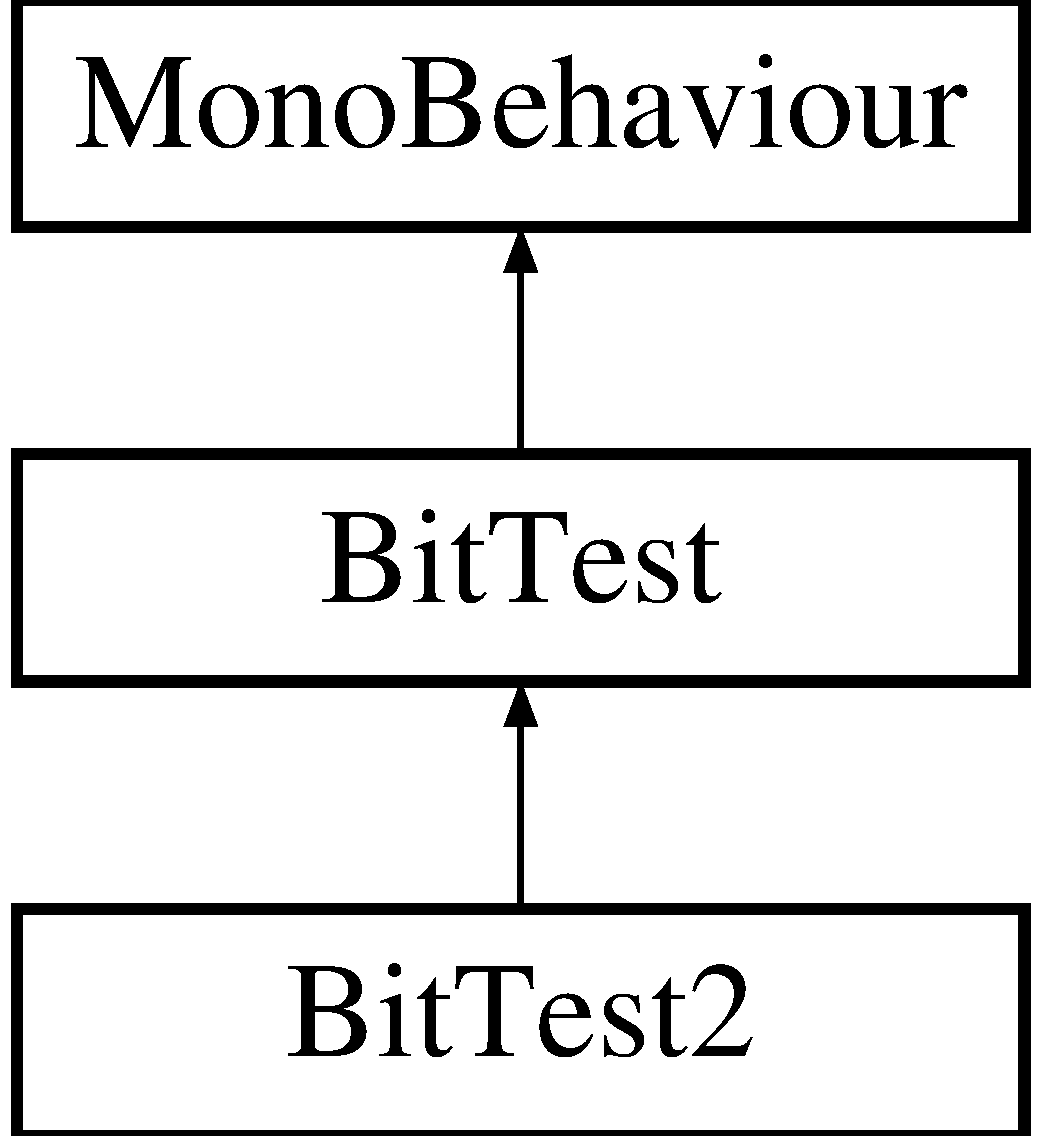
\includegraphics[height=3.000000cm]{class_bit_test2}
\end{center}
\end{figure}
\subsection*{Public Attributes}
\begin{DoxyCompactItemize}
\item 
\hypertarget{class_bit_test2_adb24602605c8f93489e0a78c52fc11c6}{string {\bfseries bit\-Test2\-Str}}\label{class_bit_test2_adb24602605c8f93489e0a78c52fc11c6}

\item 
\hypertarget{class_bit_test2_a165f84e9745d95c264b07ba5b3547161}{List$<$ int $>$ {\bfseries list1}}\label{class_bit_test2_a165f84e9745d95c264b07ba5b3547161}

\item 
\hypertarget{class_bit_test2_ace61bc6d3735c8e66d31125f1e3faa35}{List$<$ \hyperlink{class_bit_test_1_1_sereal}{Sereal} $>$ {\bfseries list2}}\label{class_bit_test2_ace61bc6d3735c8e66d31125f1e3faa35}

\item 
\hypertarget{class_bit_test2_ab4bf90367ffd77c563ab2416f3f7bdd8}{Dictionary$<$ int, string $>$ {\bfseries d1}}\label{class_bit_test2_ab4bf90367ffd77c563ab2416f3f7bdd8}

\end{DoxyCompactItemize}
\subsection*{Protected Member Functions}
\begin{DoxyCompactItemize}
\item 
\hypertarget{class_bit_test2_a771a1f26d53e4c517c699a8f3b7d0030}{override void {\bfseries init} ()}\label{class_bit_test2_a771a1f26d53e4c517c699a8f3b7d0030}

\item 
\hypertarget{class_bit_test2_a8cb95cc5e19810422c02ae5cb6cbebb7}{override void {\bfseries clear} ()}\label{class_bit_test2_a8cb95cc5e19810422c02ae5cb6cbebb7}

\item 
\hypertarget{class_bit_test2_a6b18710da1118238f4d184b14094ab17}{override void {\bfseries report} ()}\label{class_bit_test2_a6b18710da1118238f4d184b14094ab17}

\end{DoxyCompactItemize}


The documentation for this class was generated from the following file\-:\begin{DoxyCompactItemize}
\item 
/home/travis/build/temportalflux/\-Champ\-Net/\-Unity/\-Assets/\-Scripts/\-Attribute/Bit\-Test2.\-cs\end{DoxyCompactItemize}

\hypertarget{class_camera_blit}{\section{Camera\-Blit Class Reference}
\label{class_camera_blit}\index{Camera\-Blit@{Camera\-Blit}}
}
Inheritance diagram for Camera\-Blit\-:\begin{figure}[H]
\begin{center}
\leavevmode
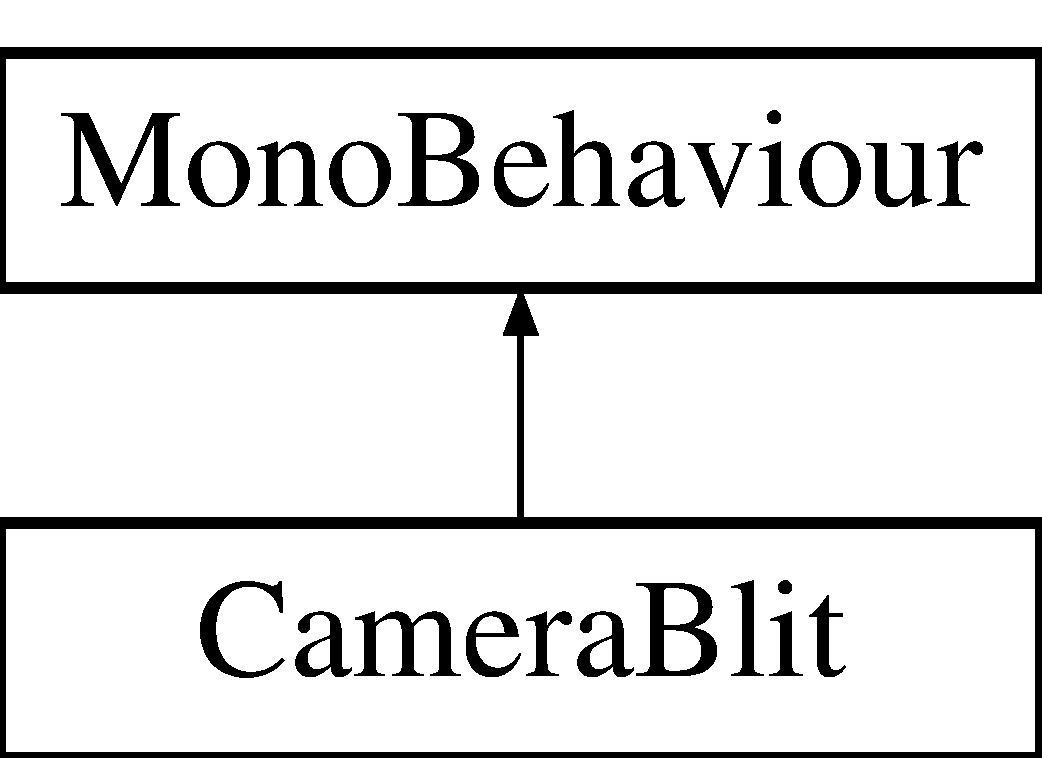
\includegraphics[height=2.000000cm]{class_camera_blit}
\end{center}
\end{figure}
\subsection*{Static Public Member Functions}
\begin{DoxyCompactItemize}
\item 
\hypertarget{class_camera_blit_a0d8bd77c40b169eac2ce9322d543d586}{static void {\bfseries set\-Material} (Material material)}\label{class_camera_blit_a0d8bd77c40b169eac2ce9322d543d586}

\end{DoxyCompactItemize}


The documentation for this class was generated from the following file\-:\begin{DoxyCompactItemize}
\item 
/home/travis/build/temportalflux/\-Champ\-Net/\-Unity/\-Assets/\-Scripts/\-Transitions/Camera\-Blit.\-cs\end{DoxyCompactItemize}

\hypertarget{class_camera_controller}{\section{Camera\-Controller Class Reference}
\label{class_camera_controller}\index{Camera\-Controller@{Camera\-Controller}}
}
Inheritance diagram for Camera\-Controller\-:\begin{figure}[H]
\begin{center}
\leavevmode
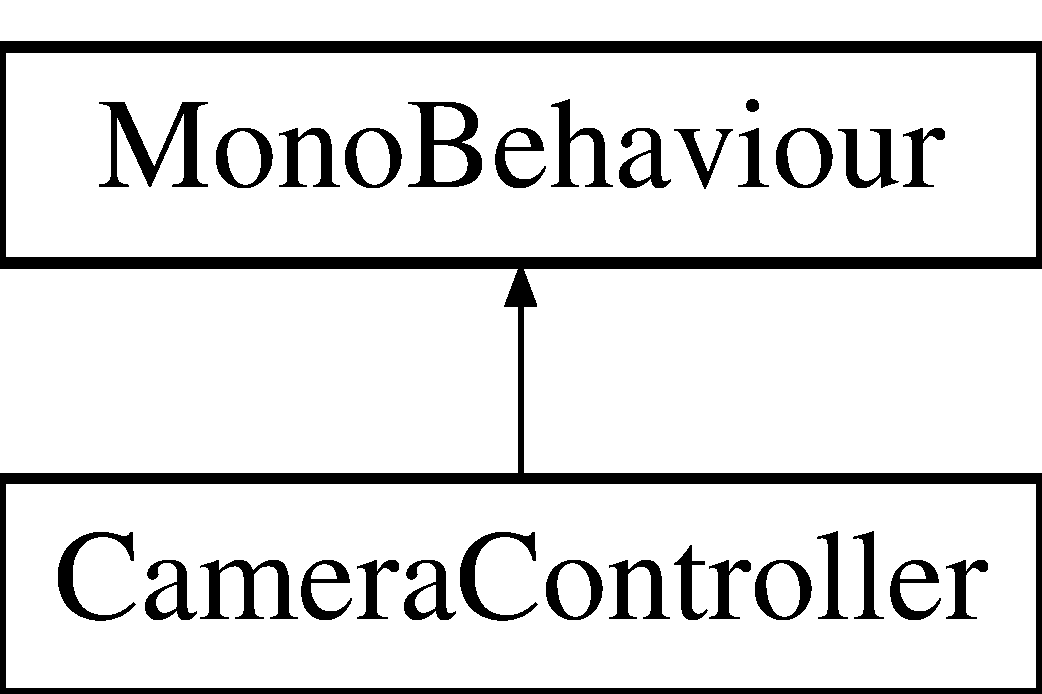
\includegraphics[height=2.000000cm]{class_camera_controller}
\end{center}
\end{figure}
\subsection*{Public Attributes}
\begin{DoxyCompactItemize}
\item 
\hypertarget{class_camera_controller_ac1525290b1ff45e8911b5c35cd869d66}{Transform {\bfseries cam}}\label{class_camera_controller_ac1525290b1ff45e8911b5c35cd869d66}

\item 
\hypertarget{class_camera_controller_a0a48b454b4a2bb8dbfc08e64b8c3e8e6}{Transform {\bfseries target}}\label{class_camera_controller_a0a48b454b4a2bb8dbfc08e64b8c3e8e6}

\item 
\hypertarget{class_camera_controller_a278961a2872dad91443d5dac07c30a2f}{float {\bfseries lerp\-Percentage}}\label{class_camera_controller_a278961a2872dad91443d5dac07c30a2f}

\end{DoxyCompactItemize}


The documentation for this class was generated from the following file\-:\begin{DoxyCompactItemize}
\item 
/home/travis/build/temportalflux/\-Champ\-Net/\-Unity/\-Assets/\-Scripts/\-Player/Camera\-Controller.\-cs\end{DoxyCompactItemize}

\hypertarget{class_camera_pixel_corrector}{\section{Camera\-Pixel\-Corrector Class Reference}
\label{class_camera_pixel_corrector}\index{Camera\-Pixel\-Corrector@{Camera\-Pixel\-Corrector}}
}
Inheritance diagram for Camera\-Pixel\-Corrector\-:\begin{figure}[H]
\begin{center}
\leavevmode
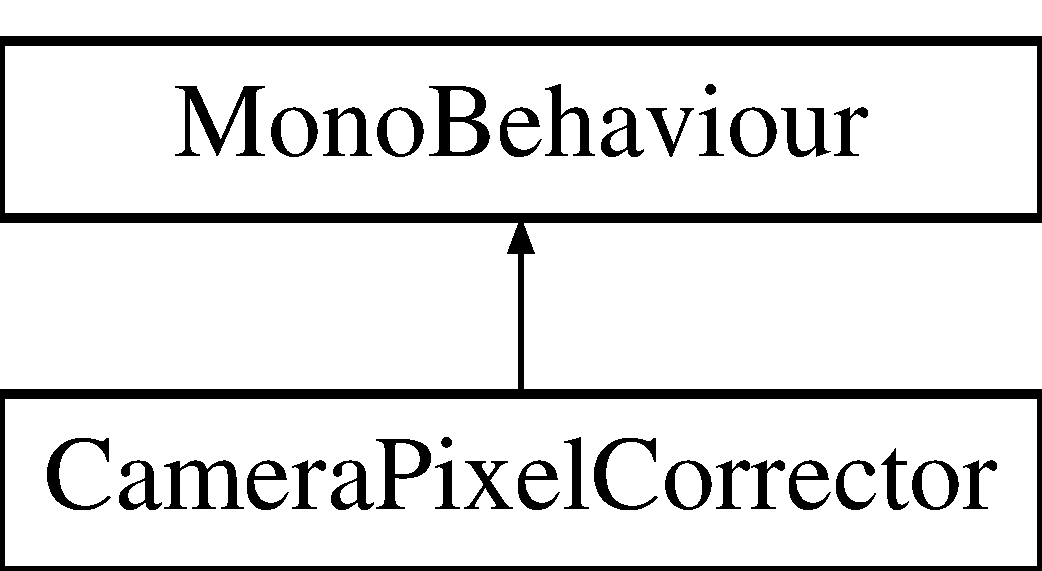
\includegraphics[height=2.000000cm]{class_camera_pixel_corrector}
\end{center}
\end{figure}
\subsection*{Public Attributes}
\begin{DoxyCompactItemize}
\item 
\hypertarget{class_camera_pixel_corrector_ad48b4a5ff5d5b30e16b7369c8d0dcdf1}{Vector2 {\bfseries target\-Viewport\-Size\-In\-Pixels} = new Vector2(480.\-0f, 320.\-0f)}\label{class_camera_pixel_corrector_ad48b4a5ff5d5b30e16b7369c8d0dcdf1}

\item 
\hypertarget{class_camera_pixel_corrector_aad6aeb12230c1e6365ff40fbccdc8029}{float {\bfseries pixels\-Per\-Unit} = 32.\-0f}\label{class_camera_pixel_corrector_aad6aeb12230c1e6365ff40fbccdc8029}

\end{DoxyCompactItemize}


The documentation for this class was generated from the following file\-:\begin{DoxyCompactItemize}
\item 
/home/travis/build/temportalflux/\-Champ\-Net/\-Unity/\-Assets/\-Scripts/\-Misc/Camera\-Pixel\-Corrector.\-cs\end{DoxyCompactItemize}

\hypertarget{class_event_battle}{\section{Event\-Battle Class Reference}
\label{class_event_battle}\index{Event\-Battle@{Event\-Battle}}
}
Inheritance diagram for Event\-Battle\-:\begin{figure}[H]
\begin{center}
\leavevmode
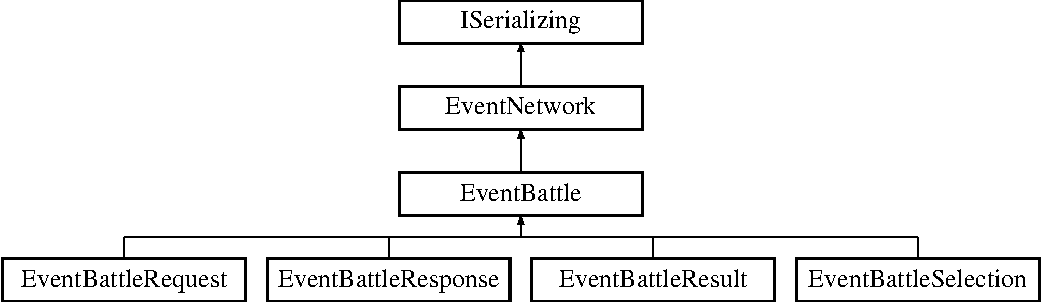
\includegraphics[height=2.083721cm]{class_event_battle}
\end{center}
\end{figure}
\subsection*{Public Member Functions}
\begin{DoxyCompactItemize}
\item 
\hypertarget{class_event_battle_a2e50e3860526edbba767018e38419e6f}{{\bfseries Event\-Battle} (byte id)}\label{class_event_battle_a2e50e3860526edbba767018e38419e6f}

\end{DoxyCompactItemize}
\subsection*{Public Attributes}
\begin{DoxyCompactItemize}
\item 
\hypertarget{class_event_battle_a0e83fdfd6da5aeb1c5f452f2ab499f78}{uint {\bfseries id\-Sender}}\label{class_event_battle_a0e83fdfd6da5aeb1c5f452f2ab499f78}

\item 
\hypertarget{class_event_battle_a9c9705b0dc0d1789a0eaabacfdc1cc61}{uint {\bfseries id\-Receiver}}\label{class_event_battle_a9c9705b0dc0d1789a0eaabacfdc1cc61}

\end{DoxyCompactItemize}
\subsection*{Additional Inherited Members}


The documentation for this class was generated from the following file\-:\begin{DoxyCompactItemize}
\item 
/home/travis/build/temportalflux/\-Champ\-Net/\-Unity/\-Assets/\-Scripts/\-Network/events/Event\-Battle.\-cs\end{DoxyCompactItemize}

\hypertarget{class_event_battle_local_start}{\section{Event\-Battle\-Local\-Start Class Reference}
\label{class_event_battle_local_start}\index{Event\-Battle\-Local\-Start@{Event\-Battle\-Local\-Start}}
}
Inheritance diagram for Event\-Battle\-Local\-Start\-:\begin{figure}[H]
\begin{center}
\leavevmode
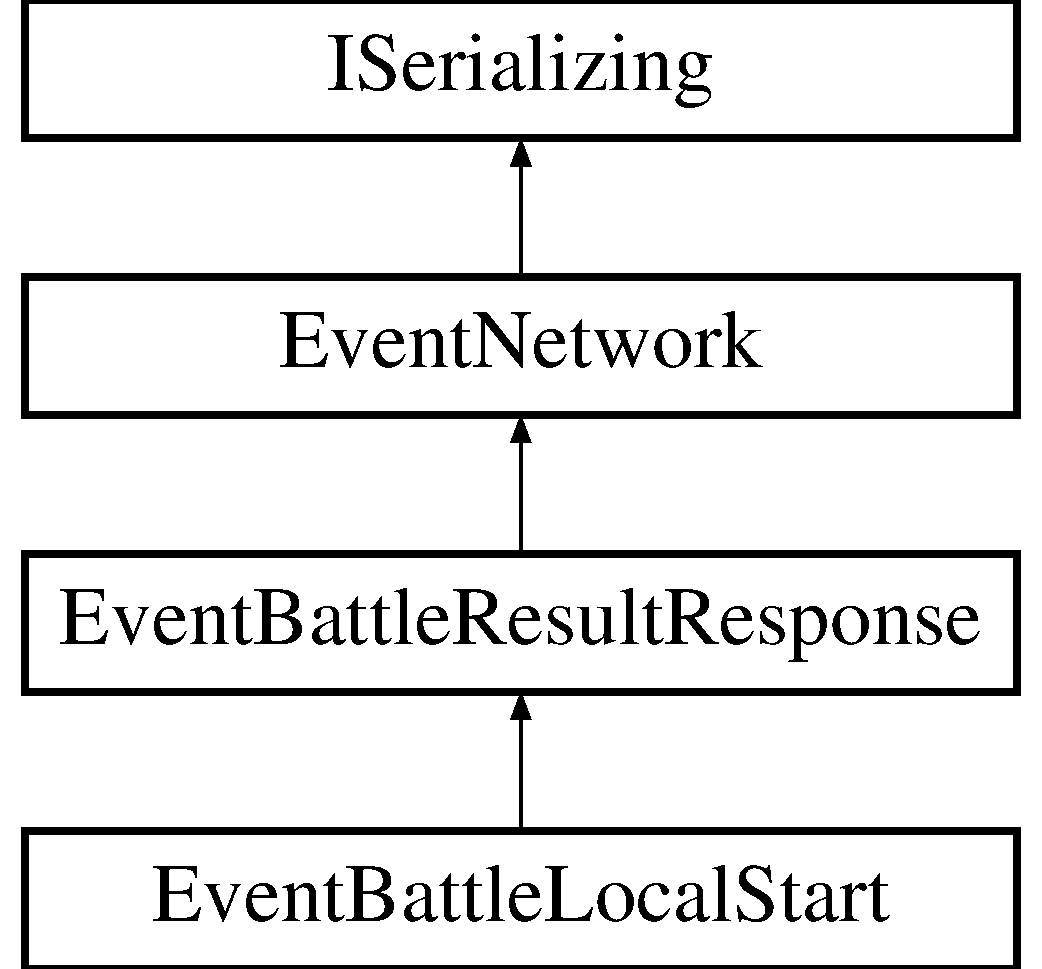
\includegraphics[height=4.000000cm]{class_event_battle_local_start}
\end{center}
\end{figure}
\subsection*{Public Member Functions}
\begin{DoxyCompactItemize}
\item 
\hypertarget{class_event_battle_local_start_a28292a2cdc78a14adc17ea50c0add8b2}{{\bfseries Event\-Battle\-Local\-Start} (uint player\-I\-D)}\label{class_event_battle_local_start_a28292a2cdc78a14adc17ea50c0add8b2}

\end{DoxyCompactItemize}
\subsection*{Additional Inherited Members}


The documentation for this class was generated from the following file\-:\begin{DoxyCompactItemize}
\item 
/home/travis/build/temportalflux/\-Champ\-Net/\-Unity/\-Assets/\-Scripts/\-Network/events/Event\-Battle\-Local\-Start.\-cs\end{DoxyCompactItemize}

\hypertarget{class_event_battle_prompt_selection}{\section{Event\-Battle\-Prompt\-Selection Class Reference}
\label{class_event_battle_prompt_selection}\index{Event\-Battle\-Prompt\-Selection@{Event\-Battle\-Prompt\-Selection}}
}
Inheritance diagram for Event\-Battle\-Prompt\-Selection\-:\begin{figure}[H]
\begin{center}
\leavevmode
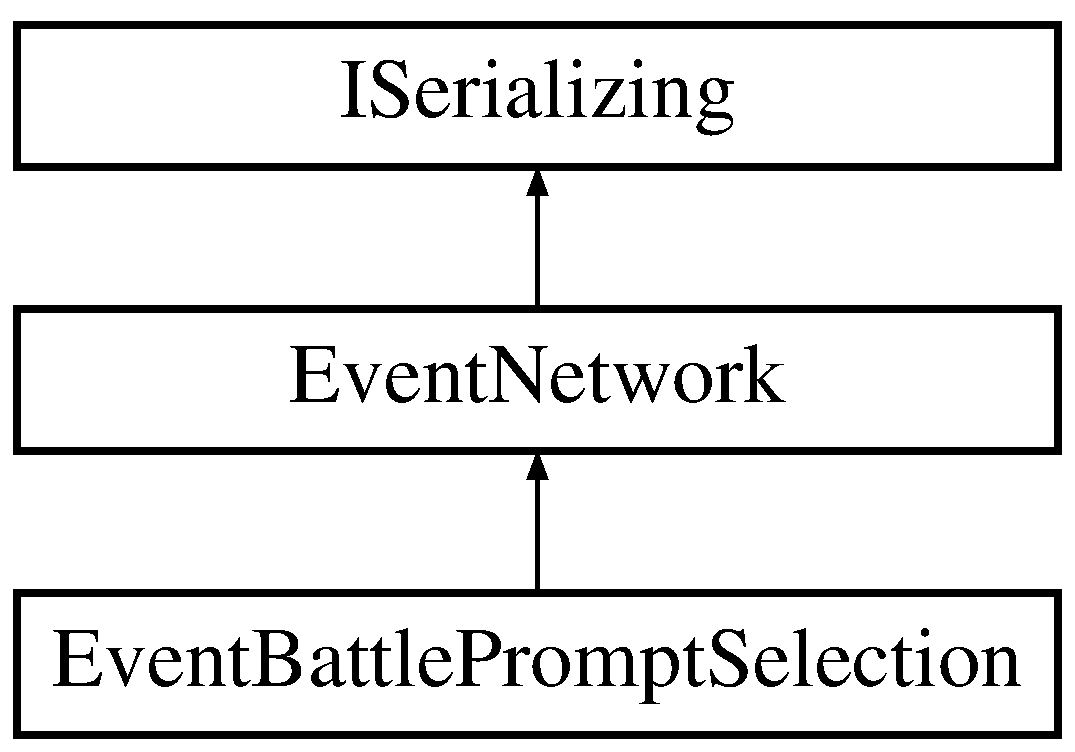
\includegraphics[height=3.000000cm]{class_event_battle_prompt_selection}
\end{center}
\end{figure}
\subsection*{Public Member Functions}
\begin{DoxyCompactItemize}
\item 
override void \hyperlink{class_event_battle_prompt_selection_aed70e58f6ae8cb1e78b7b11869faf1e5}{Execute} ()
\begin{DoxyCompactList}\small\item\em Processes this event to affect the actual environment \end{DoxyCompactList}\end{DoxyCompactItemize}
\subsection*{Public Attributes}
\begin{DoxyCompactItemize}
\item 
\hypertarget{class_event_battle_prompt_selection_a3a3a30b00d2cbb9e1fd3658667b5f0bf}{uint {\bfseries player\-A\-I\-D}}\label{class_event_battle_prompt_selection_a3a3a30b00d2cbb9e1fd3658667b5f0bf}

\item 
\hypertarget{class_event_battle_prompt_selection_adb27194b379be6543169a2a56e47eabb}{int {\bfseries \-\_\-player\-A\-Selection}}\label{class_event_battle_prompt_selection_adb27194b379be6543169a2a56e47eabb}

\item 
\hypertarget{class_event_battle_prompt_selection_a2a6c2af764a1838c48c1ecafdfc0a0f0}{int {\bfseries player\-A\-Choice}}\label{class_event_battle_prompt_selection_a2a6c2af764a1838c48c1ecafdfc0a0f0}

\item 
\hypertarget{class_event_battle_prompt_selection_ab50685401b7d5cc0491616b1515a66cb}{uint {\bfseries player\-B\-I\-D}}\label{class_event_battle_prompt_selection_ab50685401b7d5cc0491616b1515a66cb}

\item 
\hypertarget{class_event_battle_prompt_selection_acd387c1dfc6906e2c69bc9cc7e6febf6}{int {\bfseries \-\_\-player\-B\-Selection}}\label{class_event_battle_prompt_selection_acd387c1dfc6906e2c69bc9cc7e6febf6}

\item 
\hypertarget{class_event_battle_prompt_selection_a7792914c7817740ed88e6d6f5f2a5356}{int {\bfseries player\-B\-Choice}}\label{class_event_battle_prompt_selection_a7792914c7817740ed88e6d6f5f2a5356}

\end{DoxyCompactItemize}
\subsection*{Properties}
\begin{DoxyCompactItemize}
\item 
\hypertarget{class_event_battle_prompt_selection_a137eb22d4fd75f6dad9c3138803b1ca2}{\hyperlink{struct_game_state_1_1_player_a9f54c5eca1e60acbaa2074e981f51615}{Game\-State.\-Player.\-Enum\-Battle\-Selection} {\bfseries player\-A\-Selection}\hspace{0.3cm}{\ttfamily  \mbox{[}get\mbox{]}}}\label{class_event_battle_prompt_selection_a137eb22d4fd75f6dad9c3138803b1ca2}

\item 
\hypertarget{class_event_battle_prompt_selection_a4c9ef4993da9b8ca79ef969eef61c2e4}{\hyperlink{struct_game_state_1_1_player_a9f54c5eca1e60acbaa2074e981f51615}{Game\-State.\-Player.\-Enum\-Battle\-Selection} {\bfseries player\-B\-Selection}\hspace{0.3cm}{\ttfamily  \mbox{[}get\mbox{]}}}\label{class_event_battle_prompt_selection_a4c9ef4993da9b8ca79ef969eef61c2e4}

\end{DoxyCompactItemize}
\subsection*{Additional Inherited Members}


\subsection{Member Function Documentation}
\hypertarget{class_event_battle_prompt_selection_aed70e58f6ae8cb1e78b7b11869faf1e5}{\index{Event\-Battle\-Prompt\-Selection@{Event\-Battle\-Prompt\-Selection}!Execute@{Execute}}
\index{Execute@{Execute}!EventBattlePromptSelection@{Event\-Battle\-Prompt\-Selection}}
\subsubsection[{Execute}]{\setlength{\rightskip}{0pt plus 5cm}override void Event\-Battle\-Prompt\-Selection.\-Execute (
\begin{DoxyParamCaption}
{}
\end{DoxyParamCaption}
)\hspace{0.3cm}{\ttfamily [inline]}, {\ttfamily [virtual]}}}\label{class_event_battle_prompt_selection_aed70e58f6ae8cb1e78b7b11869faf1e5}


Processes this event to affect the actual environment 

Author\-: Dustin Yost 

Reimplemented from \hyperlink{class_event_network_aa5e94745568f3049a2b798c066087114}{Event\-Network}.



The documentation for this class was generated from the following file\-:\begin{DoxyCompactItemize}
\item 
/home/travis/build/temportalflux/\-Champ\-Net/\-Unity/\-Assets/\-Scripts/\-Network/events/Event\-Battle\-Prompt\-Selection.\-cs\end{DoxyCompactItemize}

\hypertarget{class_event_battle_request}{\section{Event\-Battle\-Request Class Reference}
\label{class_event_battle_request}\index{Event\-Battle\-Request@{Event\-Battle\-Request}}
}
Inheritance diagram for Event\-Battle\-Request\-:\begin{figure}[H]
\begin{center}
\leavevmode
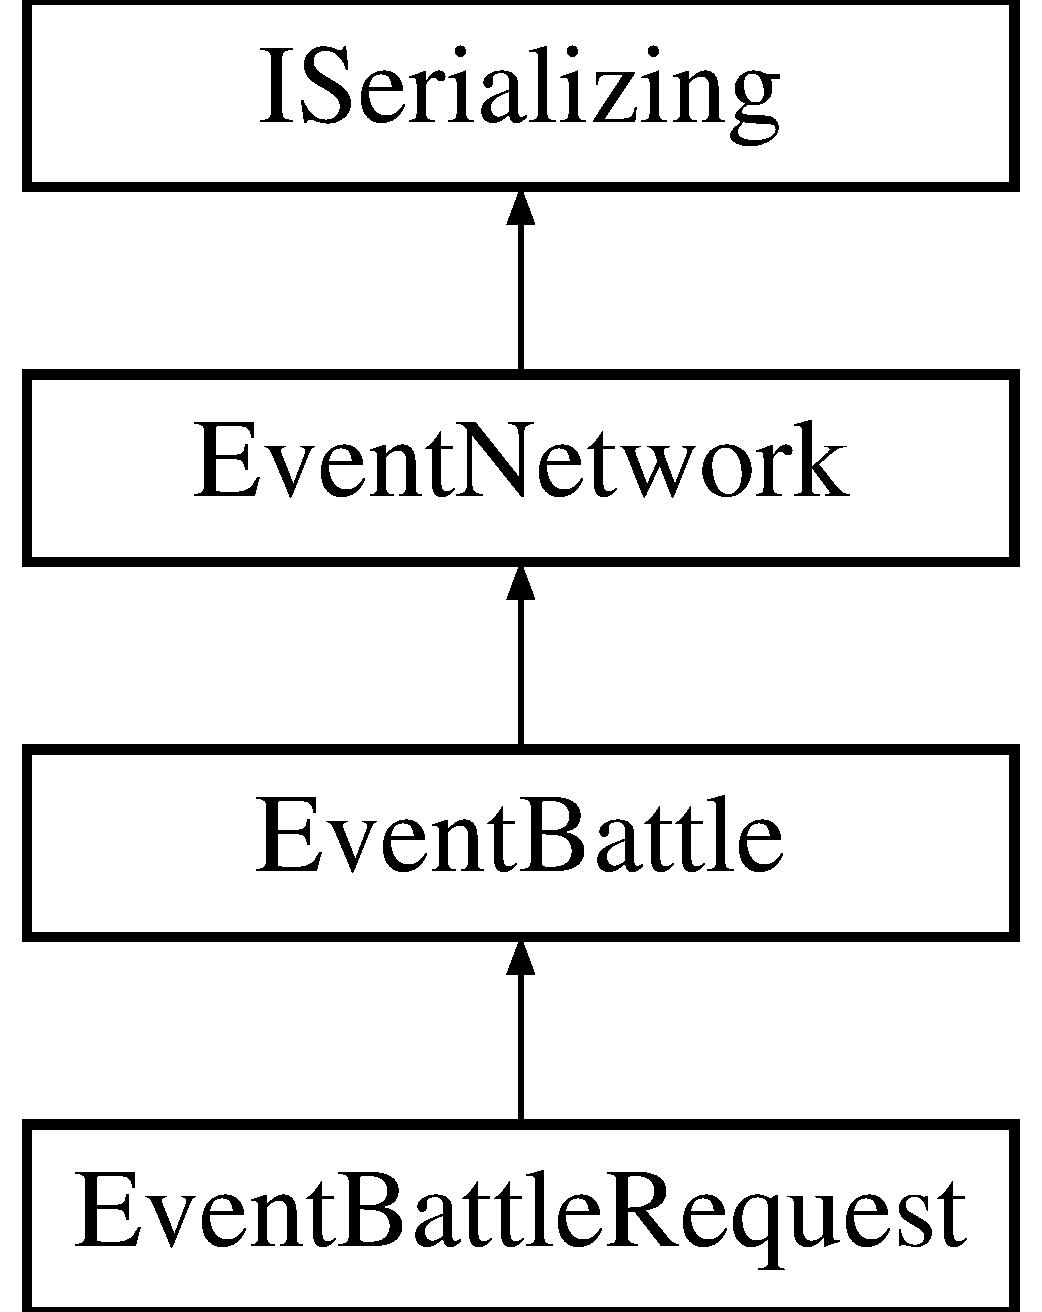
\includegraphics[height=4.000000cm]{class_event_battle_request}
\end{center}
\end{figure}
\subsection*{Public Member Functions}
\begin{DoxyCompactItemize}
\item 
\hypertarget{class_event_battle_request_a2cbe0f2890ad3fa8e00329da6fb79c8f}{{\bfseries Event\-Battle\-Request} (uint sender, uint receiver)}\label{class_event_battle_request_a2cbe0f2890ad3fa8e00329da6fb79c8f}

\item 
override void \hyperlink{class_event_battle_request_a870561ee05467ac4b18b8f9dc0370be9}{Execute} ()
\begin{DoxyCompactList}\small\item\em Processes this event to affect the actual environment \end{DoxyCompactList}\end{DoxyCompactItemize}
\subsection*{Additional Inherited Members}


\subsection{Detailed Description}
Event\-: Some player requests battle with another 

\subsection{Member Function Documentation}
\hypertarget{class_event_battle_request_a870561ee05467ac4b18b8f9dc0370be9}{\index{Event\-Battle\-Request@{Event\-Battle\-Request}!Execute@{Execute}}
\index{Execute@{Execute}!EventBattleRequest@{Event\-Battle\-Request}}
\subsubsection[{Execute}]{\setlength{\rightskip}{0pt plus 5cm}override void Event\-Battle\-Request.\-Execute (
\begin{DoxyParamCaption}
{}
\end{DoxyParamCaption}
)\hspace{0.3cm}{\ttfamily [inline]}, {\ttfamily [virtual]}}}\label{class_event_battle_request_a870561ee05467ac4b18b8f9dc0370be9}


Processes this event to affect the actual environment 

Author\-: Dustin Yost 

Reimplemented from \hyperlink{class_event_network_aa5e94745568f3049a2b798c066087114}{Event\-Network}.



The documentation for this class was generated from the following file\-:\begin{DoxyCompactItemize}
\item 
/home/travis/build/temportalflux/\-Champ\-Net/\-Unity/\-Assets/\-Scripts/\-Network/events/Event\-Battle\-Request.\-cs\end{DoxyCompactItemize}

\hypertarget{class_event_battle_response}{\section{Event\-Battle\-Response Class Reference}
\label{class_event_battle_response}\index{Event\-Battle\-Response@{Event\-Battle\-Response}}
}
Inheritance diagram for Event\-Battle\-Response\-:\begin{figure}[H]
\begin{center}
\leavevmode
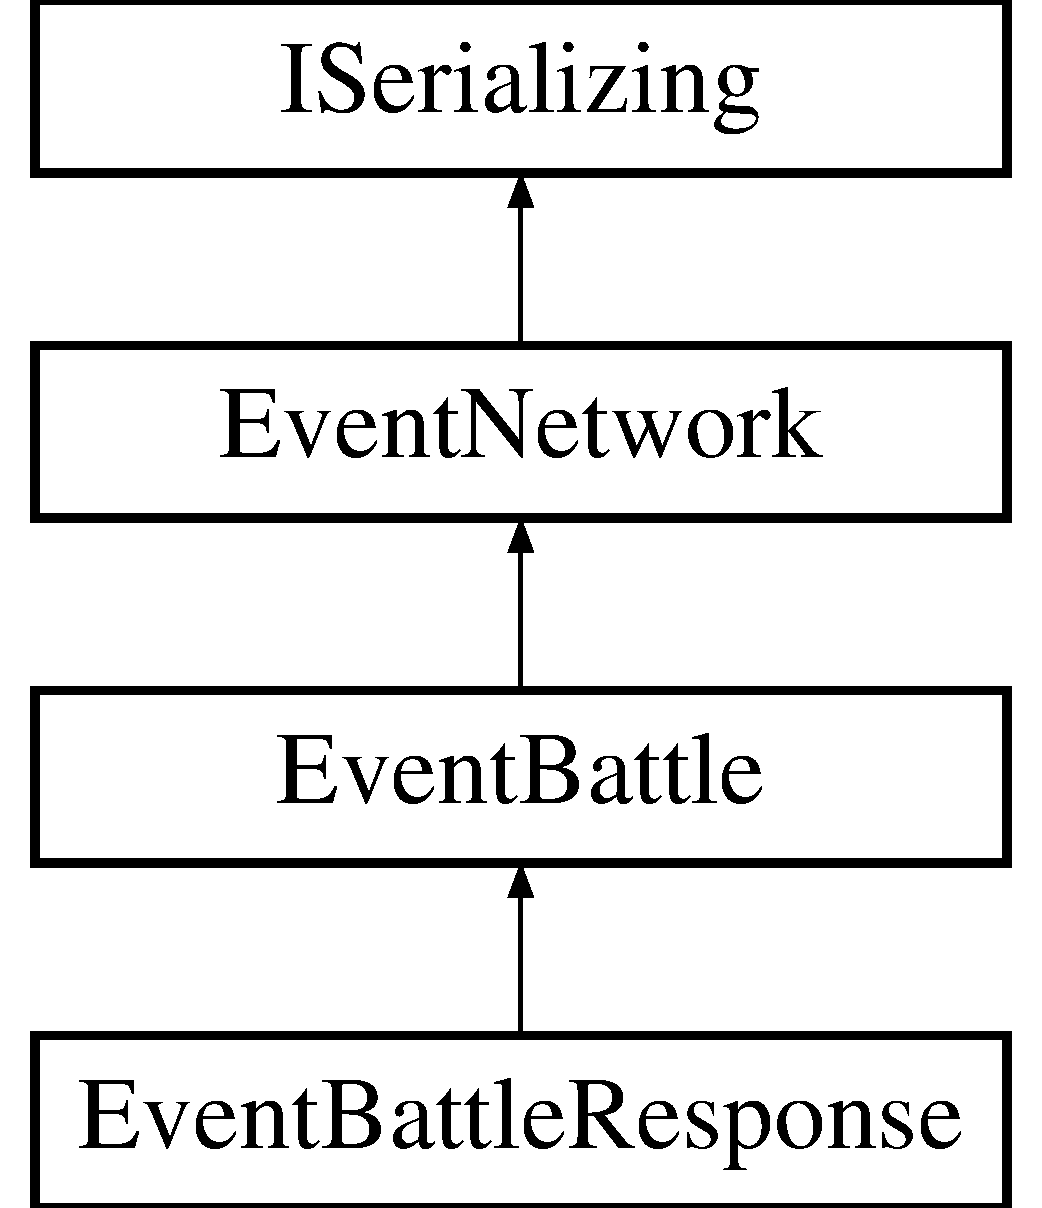
\includegraphics[height=4.000000cm]{class_event_battle_response}
\end{center}
\end{figure}
\subsection*{Public Member Functions}
\begin{DoxyCompactItemize}
\item 
\hypertarget{class_event_battle_response_a2ba1282fadb4d8f58e83b096971bb4ee}{{\bfseries Event\-Battle\-Response} (uint sender, uint receiver, bool accepted)}\label{class_event_battle_response_a2ba1282fadb4d8f58e83b096971bb4ee}

\item 
override void \hyperlink{class_event_battle_response_a3168ba71869e7eb77b6cd25165384ae8}{Execute} ()
\begin{DoxyCompactList}\small\item\em Processes this event to affect the actual environment \end{DoxyCompactList}\end{DoxyCompactItemize}
\subsection*{Public Attributes}
\begin{DoxyCompactItemize}
\item 
\hypertarget{class_event_battle_response_a43a2f73848037c9c3d67312ddadcac20}{bool {\bfseries accepted}}\label{class_event_battle_response_a43a2f73848037c9c3d67312ddadcac20}

\end{DoxyCompactItemize}
\subsection*{Additional Inherited Members}


\subsection{Detailed Description}
Event\-: Some player responds to a battle request from another player 

\subsection{Member Function Documentation}
\hypertarget{class_event_battle_response_a3168ba71869e7eb77b6cd25165384ae8}{\index{Event\-Battle\-Response@{Event\-Battle\-Response}!Execute@{Execute}}
\index{Execute@{Execute}!EventBattleResponse@{Event\-Battle\-Response}}
\subsubsection[{Execute}]{\setlength{\rightskip}{0pt plus 5cm}override void Event\-Battle\-Response.\-Execute (
\begin{DoxyParamCaption}
{}
\end{DoxyParamCaption}
)\hspace{0.3cm}{\ttfamily [inline]}, {\ttfamily [virtual]}}}\label{class_event_battle_response_a3168ba71869e7eb77b6cd25165384ae8}


Processes this event to affect the actual environment 

Author\-: Dustin Yost 

Reimplemented from \hyperlink{class_event_network_aa5e94745568f3049a2b798c066087114}{Event\-Network}.



The documentation for this class was generated from the following file\-:\begin{DoxyCompactItemize}
\item 
/home/travis/build/temportalflux/\-Champ\-Net/\-Unity/\-Assets/\-Scripts/\-Network/events/Event\-Battle\-Response.\-cs\end{DoxyCompactItemize}

\hypertarget{class_event_battle_result}{\section{Event\-Battle\-Result Class Reference}
\label{class_event_battle_result}\index{Event\-Battle\-Result@{Event\-Battle\-Result}}
}
Inheritance diagram for Event\-Battle\-Result\-:\begin{figure}[H]
\begin{center}
\leavevmode
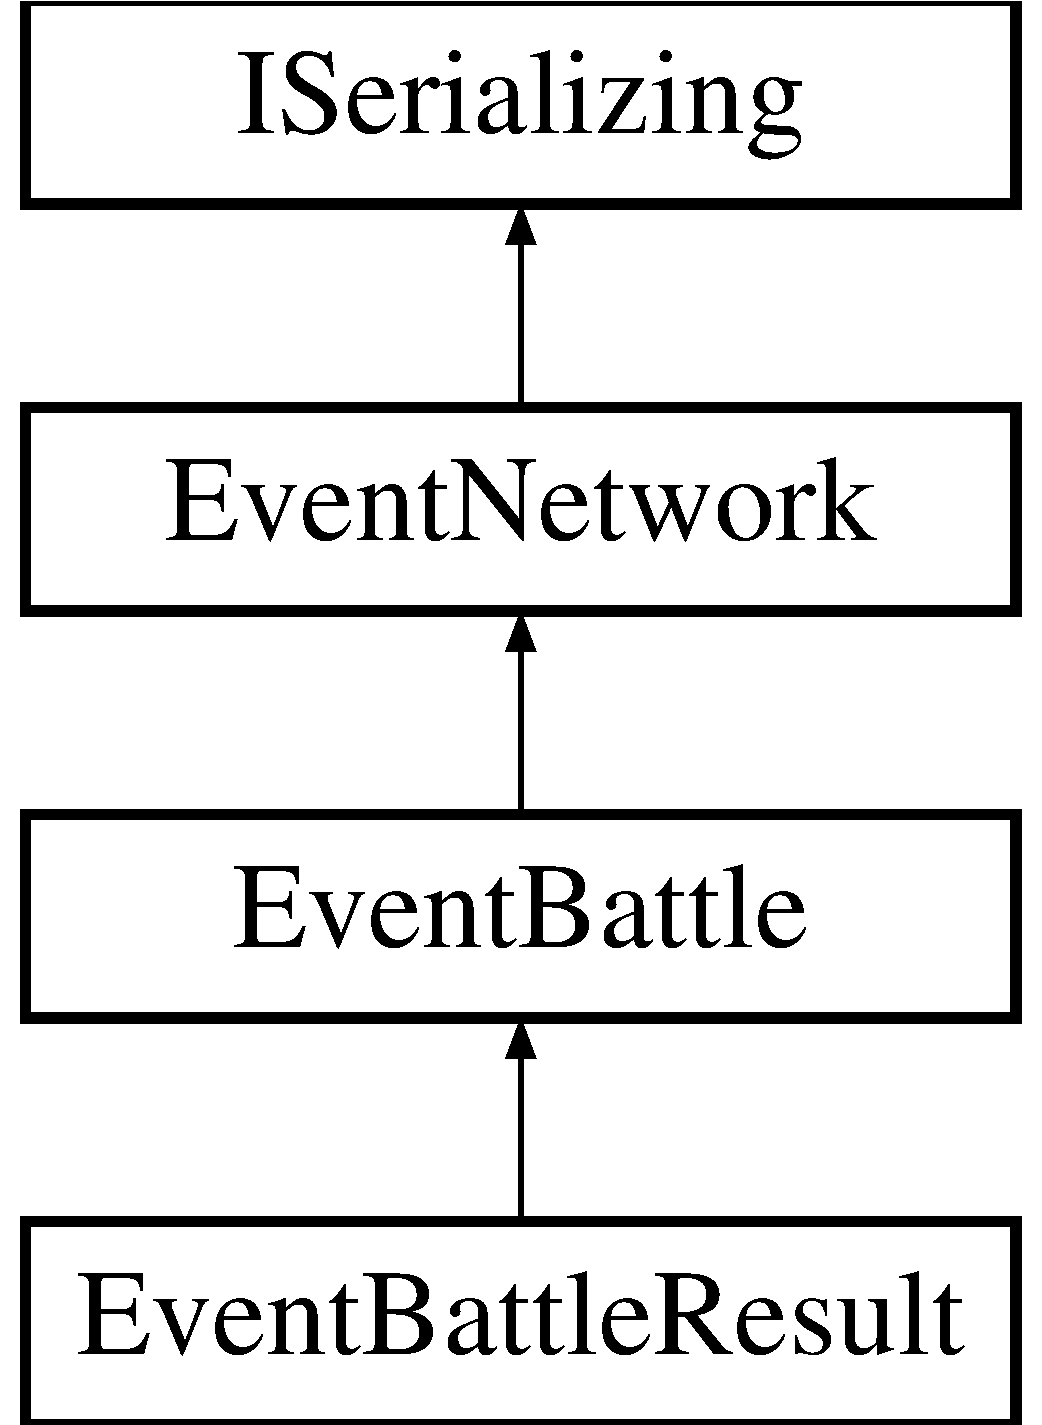
\includegraphics[height=4.000000cm]{class_event_battle_result}
\end{center}
\end{figure}
\subsection*{Public Member Functions}
\begin{DoxyCompactItemize}
\item 
\hypertarget{class_event_battle_result_a4b78976edd27a53d4cdc0edfdafbb1ec}{{\bfseries Event\-Battle\-Result} (uint winner, uint loser)}\label{class_event_battle_result_a4b78976edd27a53d4cdc0edfdafbb1ec}

\item 
override void \hyperlink{class_event_battle_result_ae2c6d5e3e01daef4de97df2e481fcac5}{Execute} ()
\begin{DoxyCompactList}\small\item\em Processes this event to affect the actual environment \end{DoxyCompactList}\end{DoxyCompactItemize}
\subsection*{Static Public Member Functions}
\begin{DoxyCompactItemize}
\item 
\hypertarget{class_event_battle_result_a3a883cf09097dbff948b90a9644b1b04}{static void {\bfseries Dispatch} (uint winner, uint loser)}\label{class_event_battle_result_a3a883cf09097dbff948b90a9644b1b04}

\end{DoxyCompactItemize}
\subsection*{Public Attributes}
\begin{DoxyCompactItemize}
\item 
\hypertarget{class_event_battle_result_a4a074620783349f4b80d301c369a0cec}{uint {\bfseries player\-I\-D\-Winner}}\label{class_event_battle_result_a4a074620783349f4b80d301c369a0cec}

\end{DoxyCompactItemize}


\subsection{Detailed Description}
Event\-: A battle has finished and the entire world needs to know about it 

\subsection{Member Function Documentation}
\hypertarget{class_event_battle_result_ae2c6d5e3e01daef4de97df2e481fcac5}{\index{Event\-Battle\-Result@{Event\-Battle\-Result}!Execute@{Execute}}
\index{Execute@{Execute}!EventBattleResult@{Event\-Battle\-Result}}
\subsubsection[{Execute}]{\setlength{\rightskip}{0pt plus 5cm}override void Event\-Battle\-Result.\-Execute (
\begin{DoxyParamCaption}
{}
\end{DoxyParamCaption}
)\hspace{0.3cm}{\ttfamily [inline]}, {\ttfamily [virtual]}}}\label{class_event_battle_result_ae2c6d5e3e01daef4de97df2e481fcac5}


Processes this event to affect the actual environment 

Author\-: Dustin Yost 

Reimplemented from \hyperlink{class_event_network_aa5e94745568f3049a2b798c066087114}{Event\-Network}.



The documentation for this class was generated from the following file\-:\begin{DoxyCompactItemize}
\item 
/home/travis/build/temportalflux/\-Champ\-Net/\-Unity/\-Assets/\-Scripts/\-Network/events/Event\-Battle\-Result.\-cs\end{DoxyCompactItemize}

\hypertarget{class_event_battle_result_response}{\section{Event\-Battle\-Result\-Response Class Reference}
\label{class_event_battle_result_response}\index{Event\-Battle\-Result\-Response@{Event\-Battle\-Result\-Response}}
}
Inheritance diagram for Event\-Battle\-Result\-Response\-:\begin{figure}[H]
\begin{center}
\leavevmode
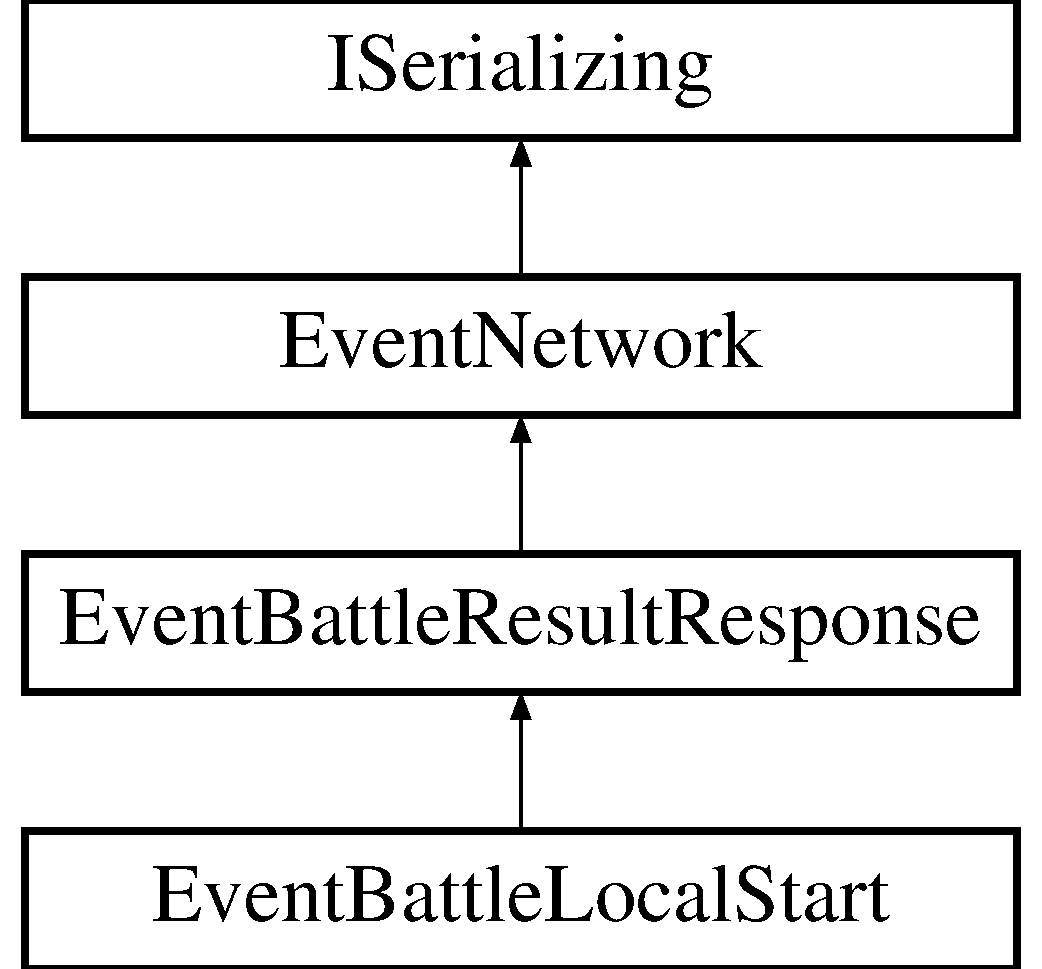
\includegraphics[height=3.000000cm]{class_event_battle_result_response}
\end{center}
\end{figure}
\subsection*{Public Attributes}
\begin{DoxyCompactItemize}
\item 
\hypertarget{class_event_battle_result_response_ada6f86b445a765ab55896a2f97a688bb}{uint {\bfseries player\-I\-D}}\label{class_event_battle_result_response_ada6f86b445a765ab55896a2f97a688bb}

\end{DoxyCompactItemize}
\subsection*{Additional Inherited Members}


The documentation for this class was generated from the following file\-:\begin{DoxyCompactItemize}
\item 
/home/travis/build/temportalflux/\-Champ\-Net/\-Unity/\-Assets/\-Scripts/\-Network/events/Event\-Battle\-Result\-Response.\-cs\end{DoxyCompactItemize}

\hypertarget{class_event_battle_selection}{\section{Event\-Battle\-Selection Class Reference}
\label{class_event_battle_selection}\index{Event\-Battle\-Selection@{Event\-Battle\-Selection}}
}
Inheritance diagram for Event\-Battle\-Selection\-:\begin{figure}[H]
\begin{center}
\leavevmode
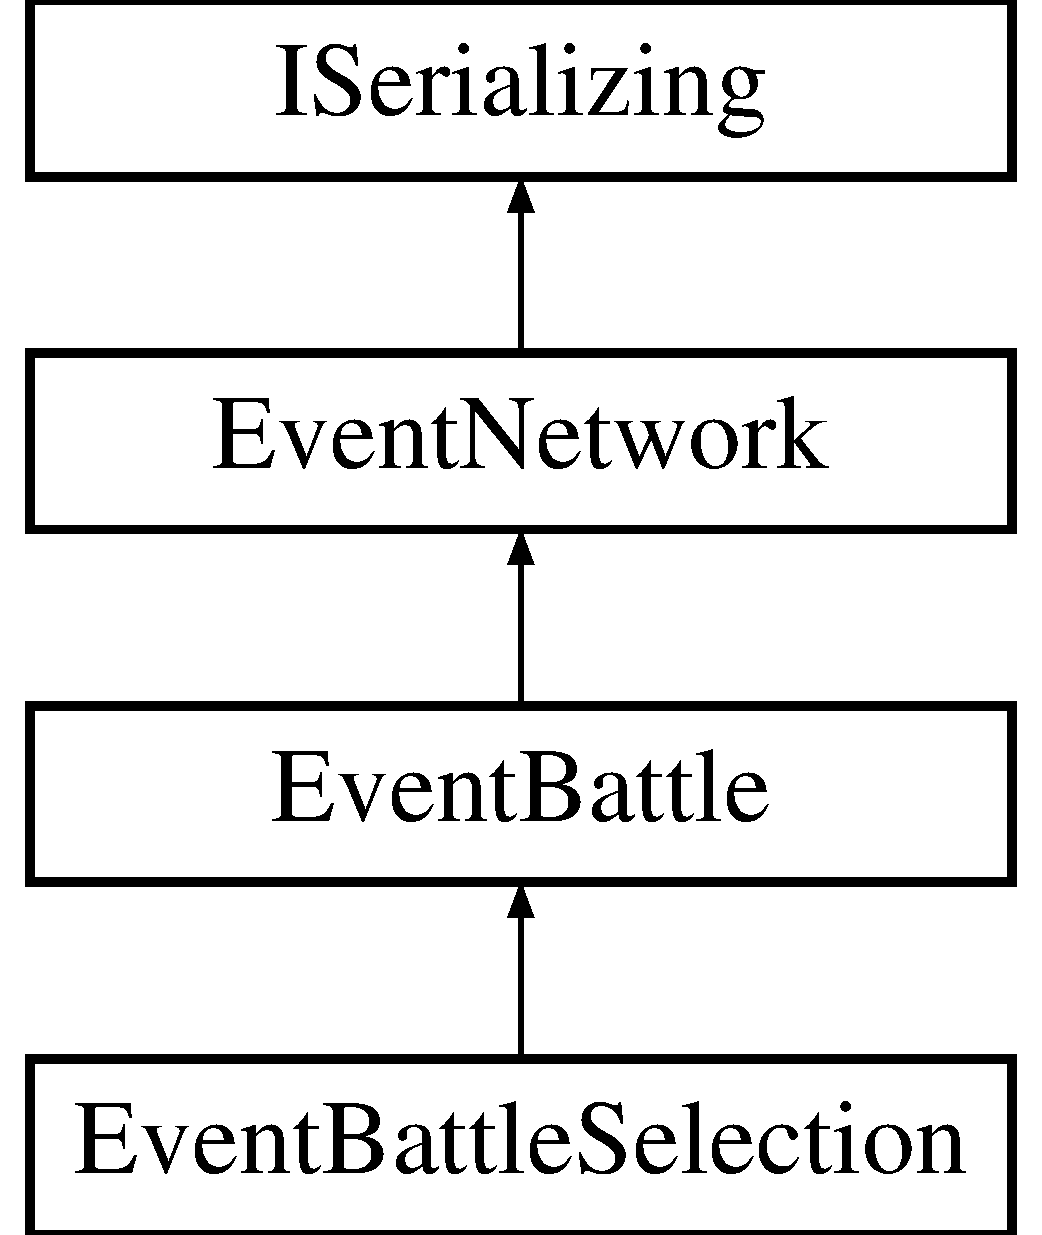
\includegraphics[height=4.000000cm]{class_event_battle_selection}
\end{center}
\end{figure}
\subsection*{Public Types}
\begin{DoxyCompactItemize}
\item 
enum {\bfseries Enum\-Selection} \{ {\bfseries A\-T\-T\-A\-C\-K}, 
{\bfseries S\-W\-A\-P}, 
{\bfseries F\-L\-E\-E}
 \}
\end{DoxyCompactItemize}
\subsection*{Public Attributes}
\begin{DoxyCompactItemize}
\item 
\hypertarget{class_event_battle_selection_a3f31e68cd024e74edbf0d8732d8d4cf6}{uint {\bfseries \-\_\-selection}}\label{class_event_battle_selection_a3f31e68cd024e74edbf0d8732d8d4cf6}

\item 
\hypertarget{class_event_battle_selection_afee34860cf0eab39082bc15a73d8e299}{uint {\bfseries choice}}\label{class_event_battle_selection_afee34860cf0eab39082bc15a73d8e299}

\end{DoxyCompactItemize}
\subsection*{Properties}
\begin{DoxyCompactItemize}
\item 
\hypertarget{class_event_battle_selection_acb6d735a144f55f502f35f3728e64fa7}{uint {\bfseries player\-Id}\hspace{0.3cm}{\ttfamily  \mbox{[}get\mbox{]}}}\label{class_event_battle_selection_acb6d735a144f55f502f35f3728e64fa7}

\item 
\hypertarget{class_event_battle_selection_a4b91cf6aadc6b2c1073413811e764903}{uint {\bfseries player\-Id\-Opponent}\hspace{0.3cm}{\ttfamily  \mbox{[}get\mbox{]}}}\label{class_event_battle_selection_a4b91cf6aadc6b2c1073413811e764903}

\item 
\hypertarget{class_event_battle_selection_abb849e7b9c472030fd4237d81cfc3111}{Enum\-Selection {\bfseries selection}\hspace{0.3cm}{\ttfamily  \mbox{[}set\mbox{]}}}\label{class_event_battle_selection_abb849e7b9c472030fd4237d81cfc3111}

\end{DoxyCompactItemize}
\subsection*{Additional Inherited Members}


The documentation for this class was generated from the following file\-:\begin{DoxyCompactItemize}
\item 
/home/travis/build/temportalflux/\-Champ\-Net/\-Unity/\-Assets/\-Scripts/\-Network/events/Event\-Battle\-Selection.\-cs\end{DoxyCompactItemize}

\hypertarget{class_event_client_joined}{\section{Event\-Client\-Joined Class Reference}
\label{class_event_client_joined}\index{Event\-Client\-Joined@{Event\-Client\-Joined}}
}
Inheritance diagram for Event\-Client\-Joined\-:\begin{figure}[H]
\begin{center}
\leavevmode
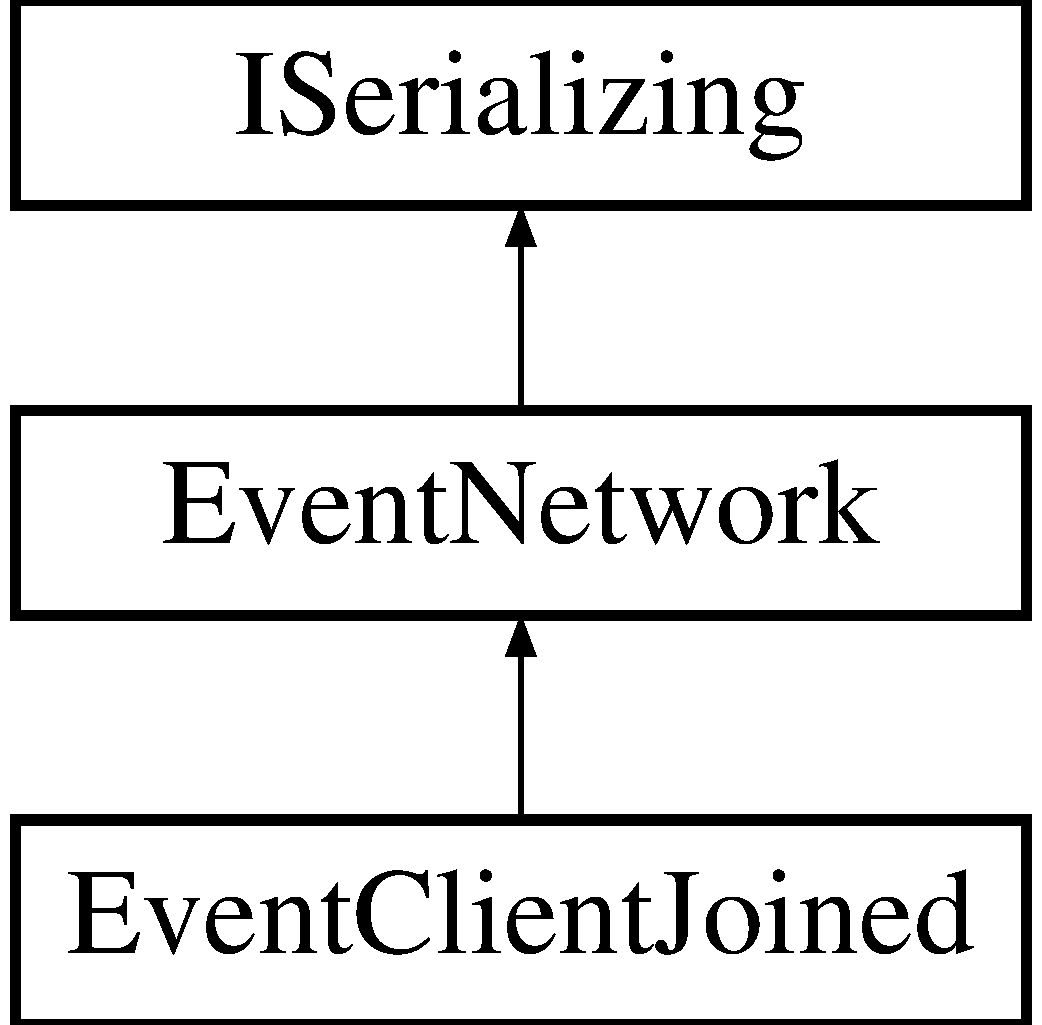
\includegraphics[height=2.000000cm]{class_event_client_joined}
\end{center}
\end{figure}
\subsection*{Public Member Functions}
\begin{DoxyCompactItemize}
\item 
\hypertarget{class_event_client_joined_adad9451ea1a292d0b4f6ce9465065bc4}{{\bfseries Event\-Client\-Joined} (Connect\-Menu.\-Player\-Descriptor\mbox{[}$\,$\mbox{]} player\-Requests)}\label{class_event_client_joined_adad9451ea1a292d0b4f6ce9465065bc4}

\item 
\hypertarget{class_event_client_joined_ad556a9c7eeb4a425ecf86ec271009241}{override int {\bfseries Get\-Size} ()}\label{class_event_client_joined_ad556a9c7eeb4a425ecf86ec271009241}

\item 
\hypertarget{class_event_client_joined_a10a9f8d247e3446fec1cc7a1eb13e6a0}{override void {\bfseries Serialize} (ref byte\mbox{[}$\,$\mbox{]} data, ref int last\-Index)}\label{class_event_client_joined_a10a9f8d247e3446fec1cc7a1eb13e6a0}

\end{DoxyCompactItemize}


\subsection{Detailed Description}
Client-\/$>$Server\-: Tell server that we joined Server-\/$>$Client\-: Tell the client of its I\-D and first player\-I\-D 

The documentation for this class was generated from the following file\-:\begin{DoxyCompactItemize}
\item 
/home/travis/build/temportalflux/\-Champ\-Net/\-Unity/\-Assets/\-Scripts/\-Network/events/Event\-Client\-Joined.\-cs\end{DoxyCompactItemize}

\hypertarget{class_event_client_left}{\section{Event\-Client\-Left Class Reference}
\label{class_event_client_left}\index{Event\-Client\-Left@{Event\-Client\-Left}}
}
Inheritance diagram for Event\-Client\-Left\-:\begin{figure}[H]
\begin{center}
\leavevmode
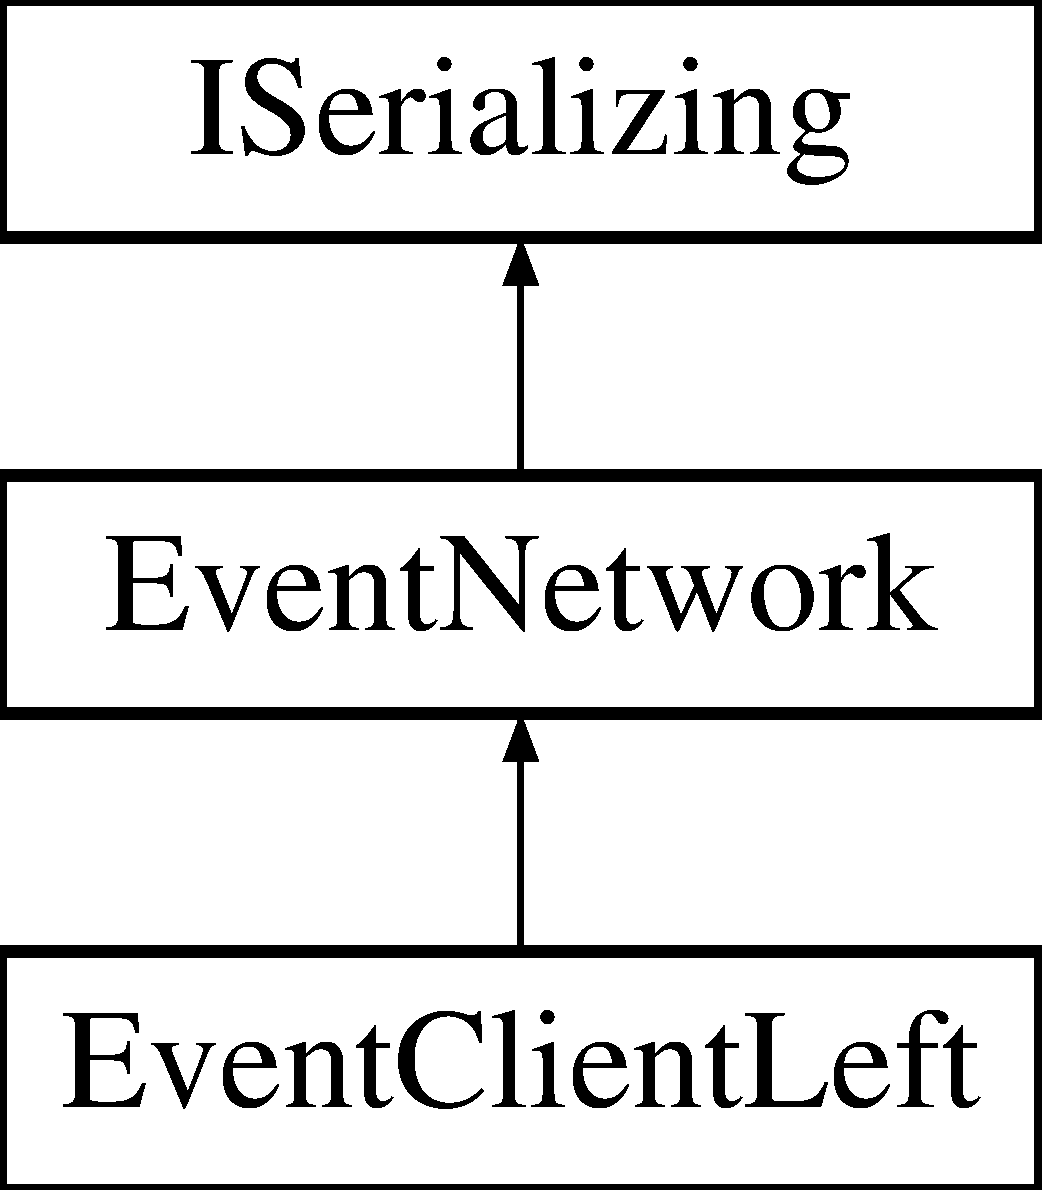
\includegraphics[height=3.000000cm]{class_event_client_left}
\end{center}
\end{figure}
\subsection*{Public Member Functions}
\begin{DoxyCompactItemize}
\item 
\hypertarget{class_event_client_left_a8e4abe7260a23d9993581f831c56ac06}{{\bfseries Event\-Client\-Left} (uint client\-I\-D)}\label{class_event_client_left_a8e4abe7260a23d9993581f831c56ac06}

\end{DoxyCompactItemize}
\subsection*{Public Attributes}
\begin{DoxyCompactItemize}
\item 
\hypertarget{class_event_client_left_a3b860c463fb45f8a4d31f5165cf2f5e9}{uint {\bfseries client\-I\-D}}\label{class_event_client_left_a3b860c463fb45f8a4d31f5165cf2f5e9}

\end{DoxyCompactItemize}
\subsection*{Additional Inherited Members}


The documentation for this class was generated from the following file\-:\begin{DoxyCompactItemize}
\item 
/home/travis/build/temportalflux/\-Champ\-Net/\-Unity/\-Assets/\-Scripts/\-Network/events/Event\-Client\-Left.\-cs\end{DoxyCompactItemize}

\hypertarget{class_event_connected}{\section{Event\-Connected Class Reference}
\label{class_event_connected}\index{Event\-Connected@{Event\-Connected}}
}


Event\-: Notification that the client has been accepted to the server  


Inheritance diagram for Event\-Connected\-:\begin{figure}[H]
\begin{center}
\leavevmode
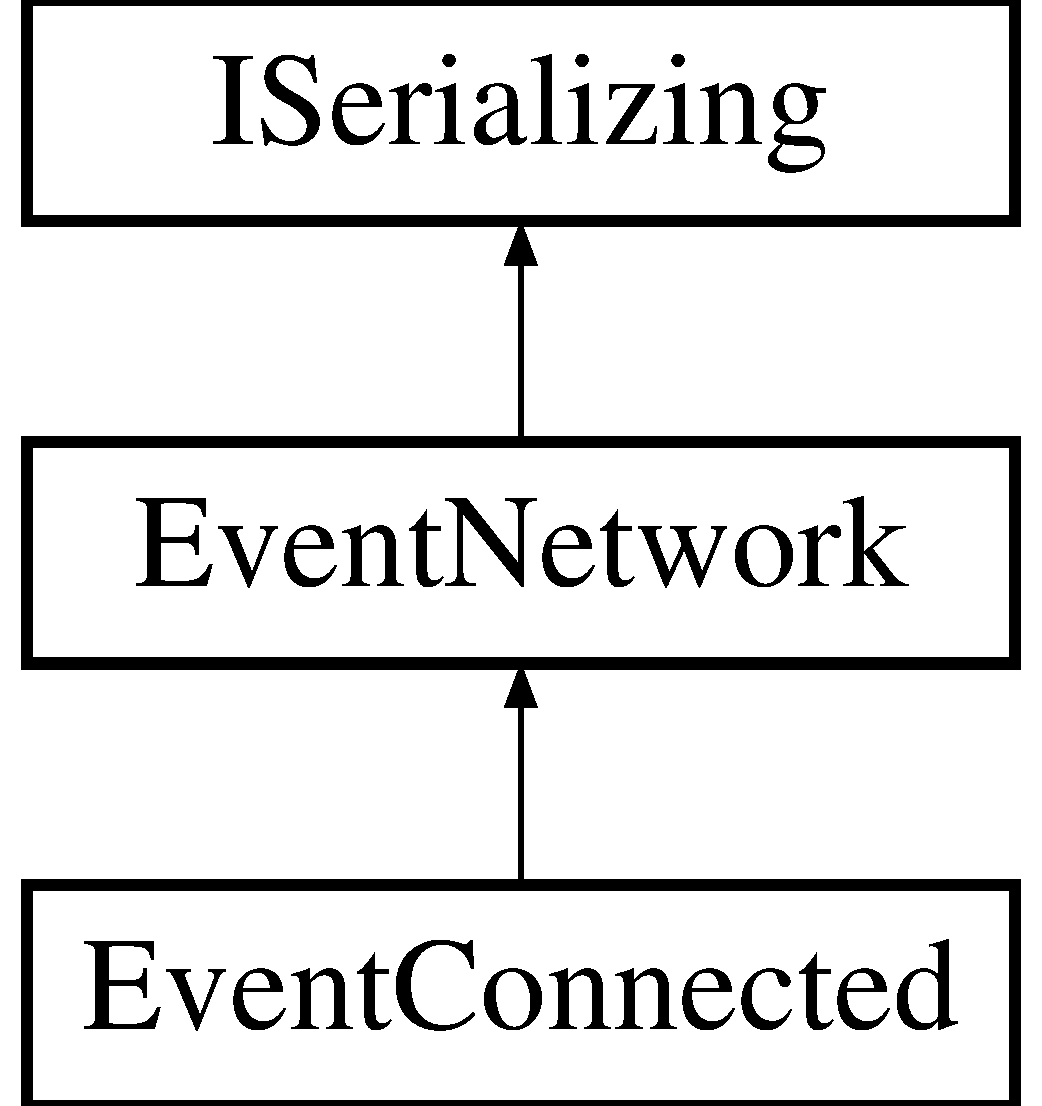
\includegraphics[height=3.000000cm]{class_event_connected}
\end{center}
\end{figure}
\subsection*{Public Member Functions}
\begin{DoxyCompactItemize}
\item 
override void \hyperlink{class_event_connected_ae8af518ac79381830f7ed283de10c82c}{Execute} ()
\begin{DoxyCompactList}\small\item\em Processes this event to affect the actual environment \end{DoxyCompactList}\end{DoxyCompactItemize}
\subsection*{Additional Inherited Members}


\subsection{Detailed Description}
Event\-: Notification that the client has been accepted to the server 

Author\-: Dustin Yost 

\subsection{Member Function Documentation}
\hypertarget{class_event_connected_ae8af518ac79381830f7ed283de10c82c}{\index{Event\-Connected@{Event\-Connected}!Execute@{Execute}}
\index{Execute@{Execute}!EventConnected@{Event\-Connected}}
\subsubsection[{Execute}]{\setlength{\rightskip}{0pt plus 5cm}override void Event\-Connected.\-Execute (
\begin{DoxyParamCaption}
{}
\end{DoxyParamCaption}
)\hspace{0.3cm}{\ttfamily [inline]}, {\ttfamily [virtual]}}}\label{class_event_connected_ae8af518ac79381830f7ed283de10c82c}


Processes this event to affect the actual environment 

Author\-: Dustin Yost 

Reimplemented from \hyperlink{class_event_network_aa5e94745568f3049a2b798c066087114}{Event\-Network}.



The documentation for this class was generated from the following file\-:\begin{DoxyCompactItemize}
\item 
/home/travis/build/temportalflux/\-Champ\-Net/\-Unity/\-Assets/\-Scripts/\-Network/events/Event\-Connected.\-cs\end{DoxyCompactItemize}

\hypertarget{class_event_connection_rejected}{\section{Event\-Connection\-Rejected Class Reference}
\label{class_event_connection_rejected}\index{Event\-Connection\-Rejected@{Event\-Connection\-Rejected}}
}


Event\-: Notification that the client has been rejected from the server  


Inheritance diagram for Event\-Connection\-Rejected\-:\begin{figure}[H]
\begin{center}
\leavevmode
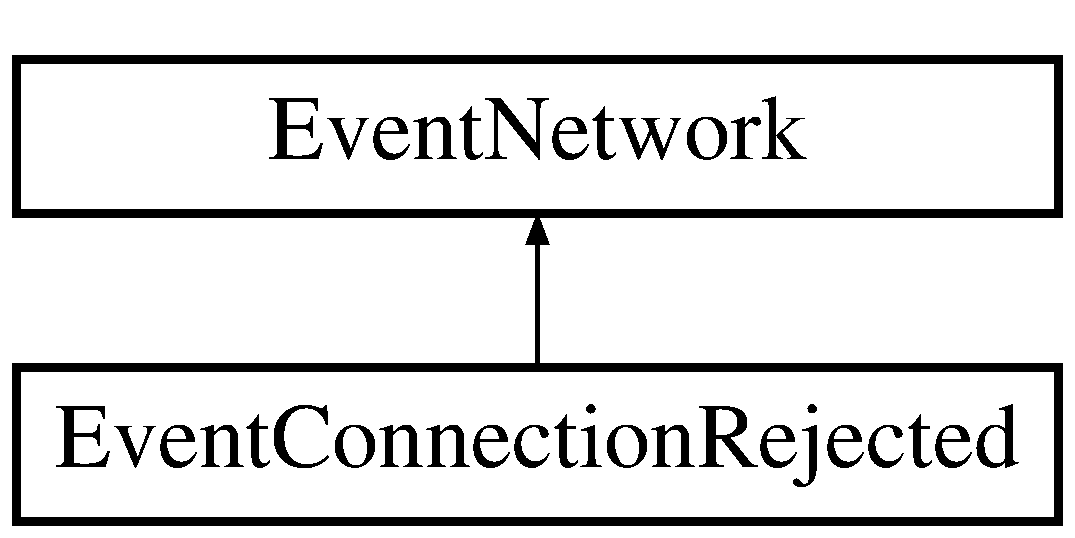
\includegraphics[height=2.000000cm]{class_event_connection_rejected}
\end{center}
\end{figure}
\subsection*{Public Member Functions}
\begin{DoxyCompactItemize}
\item 
override void \hyperlink{class_event_connection_rejected_a9d02c1d1f11f34b796a2429f6374c9ce}{Execute} ()
\begin{DoxyCompactList}\small\item\em Processes this event to affect the actual environment \end{DoxyCompactList}\end{DoxyCompactItemize}


\subsection{Detailed Description}
Event\-: Notification that the client has been rejected from the server 

Author\-: Dustin Yost 

\subsection{Member Function Documentation}
\hypertarget{class_event_connection_rejected_a9d02c1d1f11f34b796a2429f6374c9ce}{\index{Event\-Connection\-Rejected@{Event\-Connection\-Rejected}!Execute@{Execute}}
\index{Execute@{Execute}!EventConnectionRejected@{Event\-Connection\-Rejected}}
\subsubsection[{Execute}]{\setlength{\rightskip}{0pt plus 5cm}override void Event\-Connection\-Rejected.\-Execute (
\begin{DoxyParamCaption}
{}
\end{DoxyParamCaption}
)\hspace{0.3cm}{\ttfamily [inline]}}}\label{class_event_connection_rejected_a9d02c1d1f11f34b796a2429f6374c9ce}


Processes this event to affect the actual environment 

Author\-: Dustin Yost 

The documentation for this class was generated from the following file\-:\begin{DoxyCompactItemize}
\item 
/home/travis/build/temportalflux/\-Champ\-Net/\-Unity/\-Assets/\-Scripts/\-Network/events/Event\-Connected.\-cs\end{DoxyCompactItemize}

\hypertarget{class_event_disconnected}{\section{Event\-Disconnected Class Reference}
\label{class_event_disconnected}\index{Event\-Disconnected@{Event\-Disconnected}}
}
Inheritance diagram for Event\-Disconnected\-:\begin{figure}[H]
\begin{center}
\leavevmode
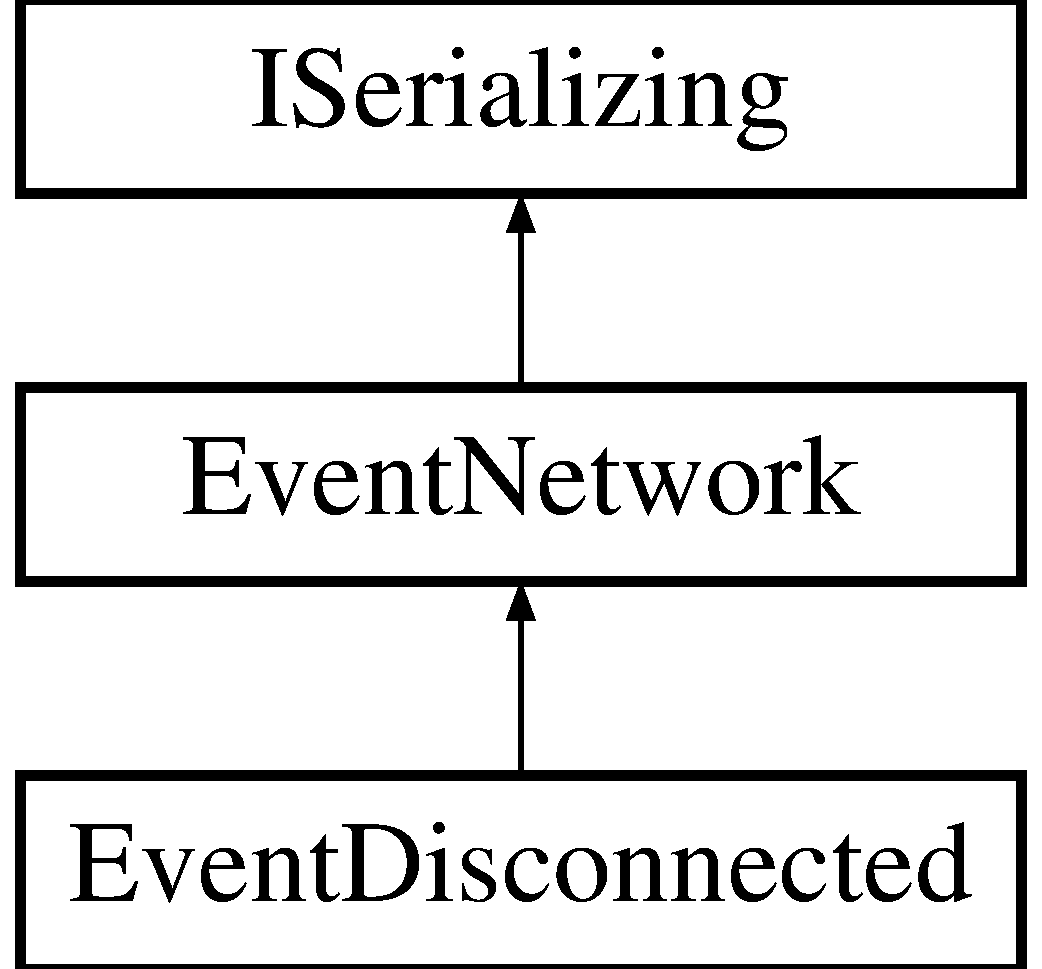
\includegraphics[height=3.000000cm]{class_event_disconnected}
\end{center}
\end{figure}
\subsection*{Public Member Functions}
\begin{DoxyCompactItemize}
\item 
override void \hyperlink{class_event_disconnected_a68523999bd55e4525522e5587ba82c3b}{Execute} ()
\begin{DoxyCompactList}\small\item\em Processes this event to affect the actual environment \end{DoxyCompactList}\end{DoxyCompactItemize}
\subsection*{Additional Inherited Members}


\subsection{Member Function Documentation}
\hypertarget{class_event_disconnected_a68523999bd55e4525522e5587ba82c3b}{\index{Event\-Disconnected@{Event\-Disconnected}!Execute@{Execute}}
\index{Execute@{Execute}!EventDisconnected@{Event\-Disconnected}}
\subsubsection[{Execute}]{\setlength{\rightskip}{0pt plus 5cm}override void Event\-Disconnected.\-Execute (
\begin{DoxyParamCaption}
{}
\end{DoxyParamCaption}
)\hspace{0.3cm}{\ttfamily [inline]}, {\ttfamily [virtual]}}}\label{class_event_disconnected_a68523999bd55e4525522e5587ba82c3b}


Processes this event to affect the actual environment 

Author\-: Dustin Yost 

Reimplemented from \hyperlink{class_event_network_aa5e94745568f3049a2b798c066087114}{Event\-Network}.



The documentation for this class was generated from the following file\-:\begin{DoxyCompactItemize}
\item 
/home/travis/build/temportalflux/\-Champ\-Net/\-Unity/\-Assets/\-Scripts/\-Network/events/Event\-Connected.\-cs\end{DoxyCompactItemize}

\hypertarget{class_event_game_state}{\section{Event\-Game\-State Class Reference}
\label{class_event_game_state}\index{Event\-Game\-State@{Event\-Game\-State}}
}


Event\-: A gamestate update  


Inheritance diagram for Event\-Game\-State\-:\begin{figure}[H]
\begin{center}
\leavevmode
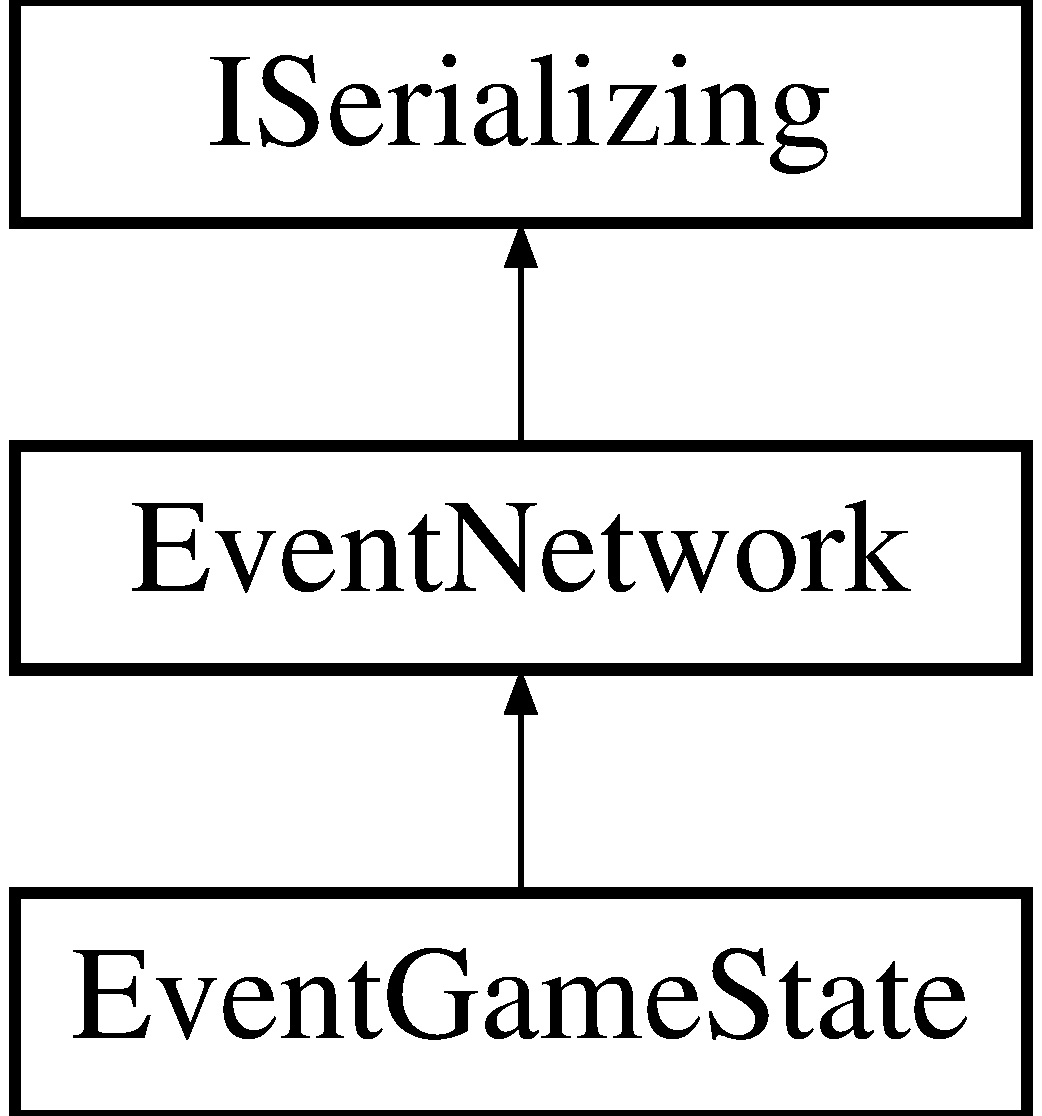
\includegraphics[height=3.000000cm]{class_event_game_state}
\end{center}
\end{figure}
\subsection*{Public Member Functions}
\begin{DoxyCompactItemize}
\item 
\hypertarget{class_event_game_state_a34fd6692a15dabe770011dfe4d65057c}{{\bfseries Event\-Game\-State} (\hyperlink{namespace_champ_net_plugin_a2ade5cfa7cf6c25ab7236c6b54a57821}{Champ\-Net\-Plugin.\-Message\-I\-Ds} message)}\label{class_event_game_state_a34fd6692a15dabe770011dfe4d65057c}

\item 
override void \hyperlink{class_event_game_state_ac8d792c7dea5e0d703d317a66bcd4cdf}{Deserialize} (byte\mbox{[}$\,$\mbox{]} data, ref int last\-Index)
\begin{DoxyCompactList}\small\item\em Deserializes data from a byte array into this event's data \end{DoxyCompactList}\item 
override void \hyperlink{class_event_game_state_a9cf710bdb22c50a1e3af2615508861b6}{Execute} ()
\begin{DoxyCompactList}\small\item\em Processes this event to affect the actual environment \end{DoxyCompactList}\end{DoxyCompactItemize}
\subsection*{Additional Inherited Members}


\subsection{Detailed Description}
Event\-: A gamestate update 

Author\-: Dustin Yost 

\subsection{Member Function Documentation}
\hypertarget{class_event_game_state_ac8d792c7dea5e0d703d317a66bcd4cdf}{\index{Event\-Game\-State@{Event\-Game\-State}!Deserialize@{Deserialize}}
\index{Deserialize@{Deserialize}!EventGameState@{Event\-Game\-State}}
\subsubsection[{Deserialize}]{\setlength{\rightskip}{0pt plus 5cm}override void Event\-Game\-State.\-Deserialize (
\begin{DoxyParamCaption}
\item[{byte\mbox{[}$\,$\mbox{]}}]{data, }
\item[{ref int}]{last\-Index}
\end{DoxyParamCaption}
)\hspace{0.3cm}{\ttfamily [inline]}, {\ttfamily [virtual]}}}\label{class_event_game_state_ac8d792c7dea5e0d703d317a66bcd4cdf}


Deserializes data from a byte array into this event's data 


\begin{DoxyParams}{Parameters}
{\em data} & The data.\\
\hline
{\em last\-Index} & The last index.\\
\hline
\end{DoxyParams}


Author\-: Dustin Yost 

Reimplemented from \hyperlink{class_event_network_af31b288f5029d8542122abe985f7df18}{Event\-Network}.

\hypertarget{class_event_game_state_a9cf710bdb22c50a1e3af2615508861b6}{\index{Event\-Game\-State@{Event\-Game\-State}!Execute@{Execute}}
\index{Execute@{Execute}!EventGameState@{Event\-Game\-State}}
\subsubsection[{Execute}]{\setlength{\rightskip}{0pt plus 5cm}override void Event\-Game\-State.\-Execute (
\begin{DoxyParamCaption}
{}
\end{DoxyParamCaption}
)\hspace{0.3cm}{\ttfamily [inline]}, {\ttfamily [virtual]}}}\label{class_event_game_state_a9cf710bdb22c50a1e3af2615508861b6}


Processes this event to affect the actual environment 

Author\-: Dustin Yost 

Reimplemented from \hyperlink{class_event_network_aa5e94745568f3049a2b798c066087114}{Event\-Network}.



The documentation for this class was generated from the following file\-:\begin{DoxyCompactItemize}
\item 
/home/travis/build/temportalflux/\-Champ\-Net/\-Unity/\-Assets/\-Scripts/\-Network/events/Event\-Game\-State.\-cs\end{DoxyCompactItemize}

\hypertarget{class_event_network}{\section{Event\-Network Class Reference}
\label{class_event_network}\index{Event\-Network@{Event\-Network}}
}


A base class for network events \href{https://msdn.microsoft.com/en-us/library/system.runtime.interopservices.unmanagedtype(v=vs.110).aspx}{\tt https\-://msdn.\-microsoft.\-com/en-\/us/library/system.\-runtime.\-interopservices.\-unmanagedtype(v=vs.\-110).\-aspx}  


Inheritance diagram for Event\-Network\-:\begin{figure}[H]
\begin{center}
\leavevmode
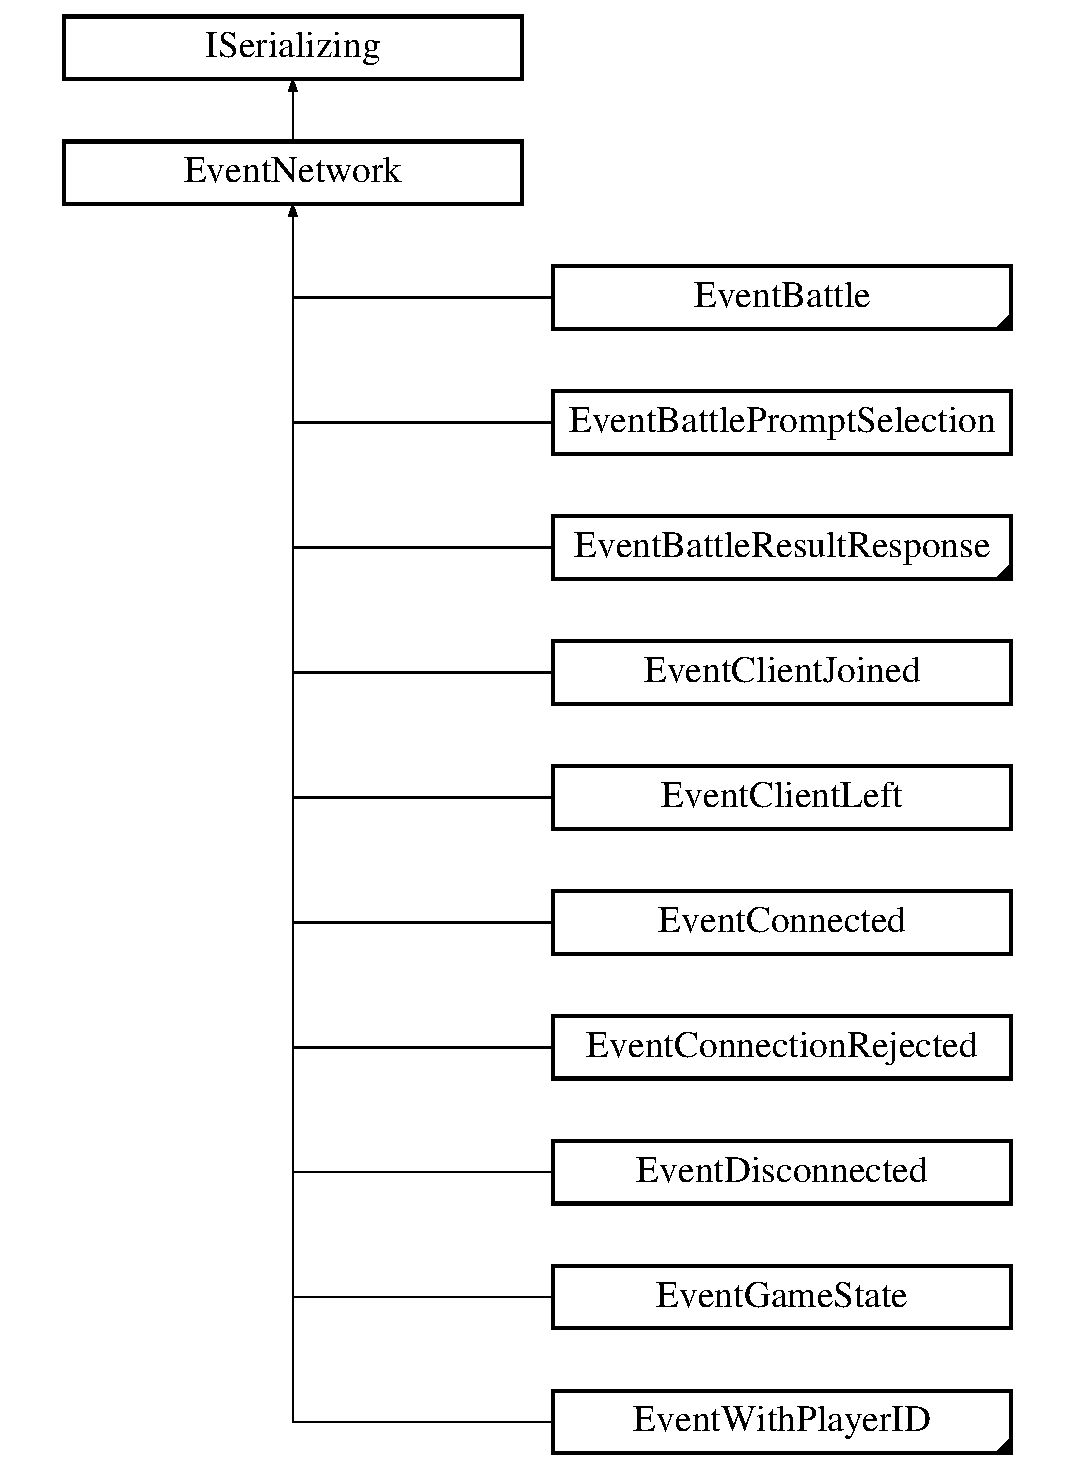
\includegraphics[height=12.000000cm]{class_event_network}
\end{center}
\end{figure}
\subsection*{Public Member Functions}
\begin{DoxyCompactItemize}
\item 
\hypertarget{class_event_network_a1f1a80ff09325571c5a27a45fb056d66}{{\bfseries Event\-Network} (byte id)}\label{class_event_network_a1f1a80ff09325571c5a27a45fb056d66}

\item 
virtual int \hyperlink{class_event_network_a627a22414c184cd4fbe4f23a25877166}{Get\-Size} ()
\begin{DoxyCompactList}\small\item\em Returns the size of the packet (the size for a potential byte\mbox{[}\mbox{]}) \end{DoxyCompactList}\item 
virtual void \hyperlink{class_event_network_af31b288f5029d8542122abe985f7df18}{Deserialize} (byte\mbox{[}$\,$\mbox{]} data, ref int last\-Index)
\begin{DoxyCompactList}\small\item\em Deserializes data from a byte array into this event's data \end{DoxyCompactList}\item 
virtual void \hyperlink{class_event_network_ae2574cdc2bb836f3e41628ff1c095238}{Serialize} (ref byte\mbox{[}$\,$\mbox{]} data, ref int last\-Index)
\begin{DoxyCompactList}\small\item\em Serializes data from this event into a byte array \end{DoxyCompactList}\item 
virtual void \hyperlink{class_event_network_aa5e94745568f3049a2b798c066087114}{Execute} ()
\begin{DoxyCompactList}\small\item\em Processes this event to affect the actual environment \end{DoxyCompactList}\end{DoxyCompactItemize}
\subsection*{Static Public Member Functions}
\begin{DoxyCompactItemize}
\item 
static \hyperlink{class_event_network}{Event\-Network} \hyperlink{class_event_network_a9cf2940f859a4c2d168fbfe83e6a19e8}{create\-Event} (int id)
\begin{DoxyCompactList}\small\item\em Creates an event from a packet identifier \end{DoxyCompactList}\item 
static void \hyperlink{class_event_network_adf54898a5ba1d6efc5f24bd58cf84b8e}{Write\-To} (ref byte\mbox{[}$\,$\mbox{]} dest, ref int offset, byte\mbox{[}$\,$\mbox{]} source)
\begin{DoxyCompactList}\small\item\em Write some byte array into another byte array at some offset \end{DoxyCompactList}\end{DoxyCompactItemize}
\subsection*{Public Attributes}
\begin{DoxyCompactItemize}
\item 
byte \hyperlink{class_event_network_adff900346978771c10eddbe469755039}{event\-I\-D}
\begin{DoxyCompactList}\small\item\em The event identifier (Champ\-Net\-Plugin\-::\-Message\-Ids) \end{DoxyCompactList}\item 
float \hyperlink{class_event_network_a1417c775954bdd96b119af2d4707db9e}{delta\-Time}
\begin{DoxyCompactList}\small\item\em The amount of time it took to get the packet from source to destination \end{DoxyCompactList}\end{DoxyCompactItemize}


\subsection{Detailed Description}
A base class for network events \href{https://msdn.microsoft.com/en-us/library/system.runtime.interopservices.unmanagedtype(v=vs.110).aspx}{\tt https\-://msdn.\-microsoft.\-com/en-\/us/library/system.\-runtime.\-interopservices.\-unmanagedtype(v=vs.\-110).\-aspx} 

Author\-: Dustin Yost 

\subsection{Member Function Documentation}
\hypertarget{class_event_network_a9cf2940f859a4c2d168fbfe83e6a19e8}{\index{Event\-Network@{Event\-Network}!create\-Event@{create\-Event}}
\index{create\-Event@{create\-Event}!EventNetwork@{Event\-Network}}
\subsubsection[{create\-Event}]{\setlength{\rightskip}{0pt plus 5cm}static {\bf Event\-Network} Event\-Network.\-create\-Event (
\begin{DoxyParamCaption}
\item[{int}]{id}
\end{DoxyParamCaption}
)\hspace{0.3cm}{\ttfamily [inline]}, {\ttfamily [static]}}}\label{class_event_network_a9cf2940f859a4c2d168fbfe83e6a19e8}


Creates an event from a packet identifier 


\begin{DoxyParams}{Parameters}
{\em id} & The identifier.\\
\hline
\end{DoxyParams}
\begin{DoxyReturn}{Returns}
Some \hyperlink{class_event_network}{Event\-Network} object
\end{DoxyReturn}


Author\-: Dustin Yost 
\begin{DoxyItemize}
\item 
\end{DoxyItemize}\hypertarget{class_event_network_af31b288f5029d8542122abe985f7df18}{\index{Event\-Network@{Event\-Network}!Deserialize@{Deserialize}}
\index{Deserialize@{Deserialize}!EventNetwork@{Event\-Network}}
\subsubsection[{Deserialize}]{\setlength{\rightskip}{0pt plus 5cm}virtual void Event\-Network.\-Deserialize (
\begin{DoxyParamCaption}
\item[{byte\mbox{[}$\,$\mbox{]}}]{data, }
\item[{ref int}]{last\-Index}
\end{DoxyParamCaption}
)\hspace{0.3cm}{\ttfamily [inline]}, {\ttfamily [virtual]}}}\label{class_event_network_af31b288f5029d8542122abe985f7df18}


Deserializes data from a byte array into this event's data 


\begin{DoxyParams}{Parameters}
{\em data} & The data.\\
\hline
{\em last\-Index} & The last index.\\
\hline
\end{DoxyParams}


Author\-: Dustin Yost 

Implements \hyperlink{interface_i_serializing_a92f8ba3a06d21e7b01e37411e4e3145c}{I\-Serializing}.



Reimplemented in \hyperlink{class_event_game_state_ac8d792c7dea5e0d703d317a66bcd4cdf}{Event\-Game\-State}.

\hypertarget{class_event_network_aa5e94745568f3049a2b798c066087114}{\index{Event\-Network@{Event\-Network}!Execute@{Execute}}
\index{Execute@{Execute}!EventNetwork@{Event\-Network}}
\subsubsection[{Execute}]{\setlength{\rightskip}{0pt plus 5cm}virtual void Event\-Network.\-Execute (
\begin{DoxyParamCaption}
{}
\end{DoxyParamCaption}
)\hspace{0.3cm}{\ttfamily [inline]}, {\ttfamily [virtual]}}}\label{class_event_network_aa5e94745568f3049a2b798c066087114}


Processes this event to affect the actual environment 

Author\-: Dustin Yost 

Reimplemented in \hyperlink{class_event_disconnected_a68523999bd55e4525522e5587ba82c3b}{Event\-Disconnected}, \hyperlink{class_event_connection_rejected_a9d02c1d1f11f34b796a2429f6374c9ce}{Event\-Connection\-Rejected}, \hyperlink{class_event_battle_prompt_selection_aed70e58f6ae8cb1e78b7b11869faf1e5}{Event\-Battle\-Prompt\-Selection}, \hyperlink{class_event_game_state_a9cf710bdb22c50a1e3af2615508861b6}{Event\-Game\-State}, \hyperlink{class_event_battle_result_ae2c6d5e3e01daef4de97df2e481fcac5}{Event\-Battle\-Result}, \hyperlink{class_event_connected_ae8af518ac79381830f7ed283de10c82c}{Event\-Connected}, \hyperlink{class_event_battle_response_a3168ba71869e7eb77b6cd25165384ae8}{Event\-Battle\-Response}, \hyperlink{class_event_battle_request_a870561ee05467ac4b18b8f9dc0370be9}{Event\-Battle\-Request}, and \hyperlink{class_event_battle_opponent_disconnected_aa08461a61a0c80ee3cb37b488af30e00}{Event\-Battle\-Opponent\-Disconnected}.

\hypertarget{class_event_network_a627a22414c184cd4fbe4f23a25877166}{\index{Event\-Network@{Event\-Network}!Get\-Size@{Get\-Size}}
\index{Get\-Size@{Get\-Size}!EventNetwork@{Event\-Network}}
\subsubsection[{Get\-Size}]{\setlength{\rightskip}{0pt plus 5cm}virtual int Event\-Network.\-Get\-Size (
\begin{DoxyParamCaption}
{}
\end{DoxyParamCaption}
)\hspace{0.3cm}{\ttfamily [inline]}, {\ttfamily [virtual]}}}\label{class_event_network_a627a22414c184cd4fbe4f23a25877166}


Returns the size of the packet (the size for a potential byte\mbox{[}\mbox{]}) 

\begin{DoxyReturn}{Returns}
the integer length of a byte array to hold this event's data
\end{DoxyReturn}


Author\-: Dustin Yost 

Implements \hyperlink{interface_i_serializing_a9e6ea0afaeac8d1d57e20579f87bebe2}{I\-Serializing}.



Reimplemented in \hyperlink{class_event_client_joined_ad556a9c7eeb4a425ecf86ec271009241}{Event\-Client\-Joined}.

\hypertarget{class_event_network_ae2574cdc2bb836f3e41628ff1c095238}{\index{Event\-Network@{Event\-Network}!Serialize@{Serialize}}
\index{Serialize@{Serialize}!EventNetwork@{Event\-Network}}
\subsubsection[{Serialize}]{\setlength{\rightskip}{0pt plus 5cm}virtual void Event\-Network.\-Serialize (
\begin{DoxyParamCaption}
\item[{ref byte\mbox{[}$\,$\mbox{]}}]{data, }
\item[{ref int}]{last\-Index}
\end{DoxyParamCaption}
)\hspace{0.3cm}{\ttfamily [inline]}, {\ttfamily [virtual]}}}\label{class_event_network_ae2574cdc2bb836f3e41628ff1c095238}


Serializes data from this event into a byte array 


\begin{DoxyParams}{Parameters}
{\em data} & The data.\\
\hline
{\em last\-Index} & The last index.\\
\hline
\end{DoxyParams}


Author\-: Dustin Yost 

Implements \hyperlink{interface_i_serializing_ac31a44c2358a197e774fa3f79cc80356}{I\-Serializing}.



Reimplemented in \hyperlink{class_event_client_joined_a10a9f8d247e3446fec1cc7a1eb13e6a0}{Event\-Client\-Joined}.

\hypertarget{class_event_network_adf54898a5ba1d6efc5f24bd58cf84b8e}{\index{Event\-Network@{Event\-Network}!Write\-To@{Write\-To}}
\index{Write\-To@{Write\-To}!EventNetwork@{Event\-Network}}
\subsubsection[{Write\-To}]{\setlength{\rightskip}{0pt plus 5cm}static void Event\-Network.\-Write\-To (
\begin{DoxyParamCaption}
\item[{ref byte\mbox{[}$\,$\mbox{]}}]{dest, }
\item[{ref int}]{offset, }
\item[{byte\mbox{[}$\,$\mbox{]}}]{source}
\end{DoxyParamCaption}
)\hspace{0.3cm}{\ttfamily [inline]}, {\ttfamily [static]}}}\label{class_event_network_adf54898a5ba1d6efc5f24bd58cf84b8e}


Write some byte array into another byte array at some offset 


\begin{DoxyParams}{Parameters}
{\em dest} & The data to copy.\\
\hline
{\em offset} & The offset in bytes.\\
\hline
{\em source} & The data object to copy into at the offset.\\
\hline
\end{DoxyParams}


Author\-: Dustin Yost 

\subsection{Member Data Documentation}
\hypertarget{class_event_network_a1417c775954bdd96b119af2d4707db9e}{\index{Event\-Network@{Event\-Network}!delta\-Time@{delta\-Time}}
\index{delta\-Time@{delta\-Time}!EventNetwork@{Event\-Network}}
\subsubsection[{delta\-Time}]{\setlength{\rightskip}{0pt plus 5cm}float Event\-Network.\-delta\-Time}}\label{class_event_network_a1417c775954bdd96b119af2d4707db9e}


The amount of time it took to get the packet from source to destination 

\hypertarget{class_event_network_adff900346978771c10eddbe469755039}{\index{Event\-Network@{Event\-Network}!event\-I\-D@{event\-I\-D}}
\index{event\-I\-D@{event\-I\-D}!EventNetwork@{Event\-Network}}
\subsubsection[{event\-I\-D}]{\setlength{\rightskip}{0pt plus 5cm}byte Event\-Network.\-event\-I\-D}}\label{class_event_network_adff900346978771c10eddbe469755039}


The event identifier (Champ\-Net\-Plugin\-::\-Message\-Ids) 

Author\-: Dustin Yost 

The documentation for this class was generated from the following file\-:\begin{DoxyCompactItemize}
\item 
/home/travis/build/temportalflux/\-Champ\-Net/\-Unity/\-Assets/\-Scripts/\-Network/events/Event\-Network.\-cs\end{DoxyCompactItemize}

\hypertarget{class_event_player_add_monster}{\section{Event\-Player\-Add\-Monster Class Reference}
\label{class_event_player_add_monster}\index{Event\-Player\-Add\-Monster@{Event\-Player\-Add\-Monster}}
}
Inheritance diagram for Event\-Player\-Add\-Monster\-:\begin{figure}[H]
\begin{center}
\leavevmode
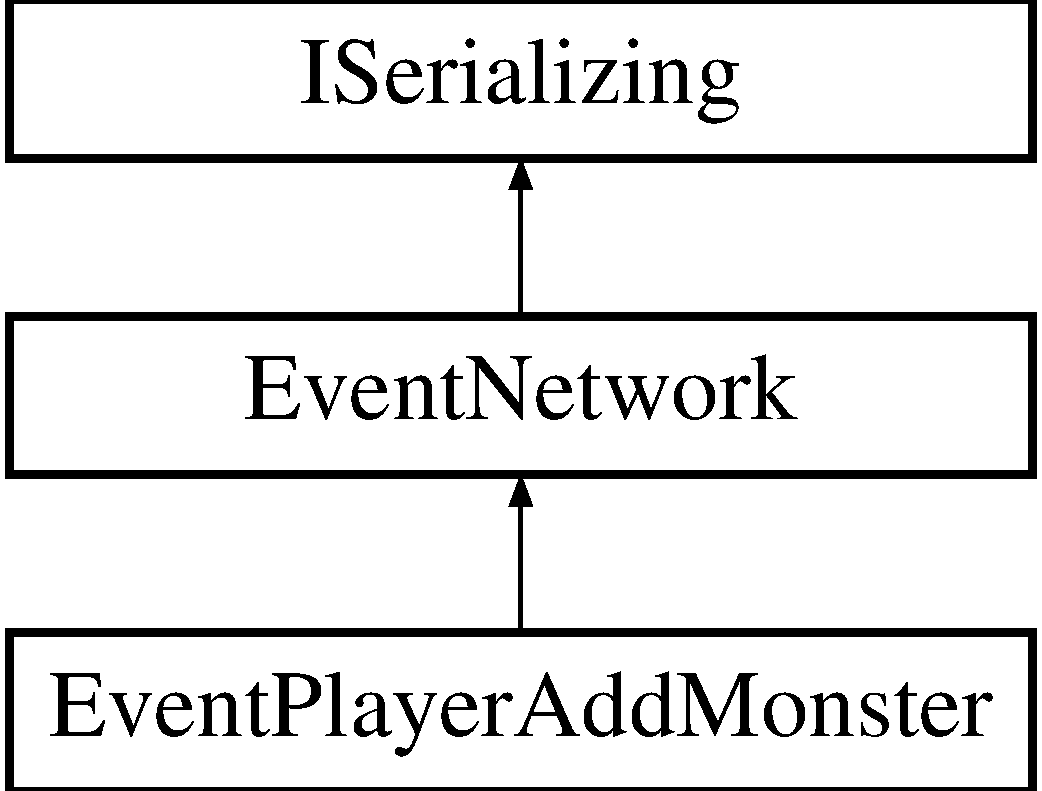
\includegraphics[height=3.000000cm]{class_event_player_add_monster}
\end{center}
\end{figure}
\subsection*{Public Member Functions}
\begin{DoxyCompactItemize}
\item 
\hypertarget{class_event_player_add_monster_a645f8b48f53de87d0346dfd713eecb41}{{\bfseries Event\-Player\-Add\-Monster} (uint player\-I\-D, uint monster\-I\-D)}\label{class_event_player_add_monster_a645f8b48f53de87d0346dfd713eecb41}

\end{DoxyCompactItemize}
\subsection*{Static Public Member Functions}
\begin{DoxyCompactItemize}
\item 
\hypertarget{class_event_player_add_monster_a56c42f47c38537ea4bb992b4dfa010ae}{static void {\bfseries Dispatch} (uint player\-I\-D, uint monster\-I\-D)}\label{class_event_player_add_monster_a56c42f47c38537ea4bb992b4dfa010ae}

\end{DoxyCompactItemize}
\subsection*{Public Attributes}
\begin{DoxyCompactItemize}
\item 
\hypertarget{class_event_player_add_monster_a4beff17ff8417fab909dd0daa4329c4c}{uint {\bfseries player\-I\-D}}\label{class_event_player_add_monster_a4beff17ff8417fab909dd0daa4329c4c}

\item 
\hypertarget{class_event_player_add_monster_ad135e14b529373022b539ed7a900d5c6}{uint {\bfseries monster\-I\-D}}\label{class_event_player_add_monster_ad135e14b529373022b539ed7a900d5c6}

\end{DoxyCompactItemize}


The documentation for this class was generated from the following file\-:\begin{DoxyCompactItemize}
\item 
/home/travis/build/temportalflux/\-Champ\-Net/\-Unity/\-Assets/\-Scripts/\-Network/events/Event\-Player\-Add\-Monster.\-cs\end{DoxyCompactItemize}

\hypertarget{class_event_request_movement}{\section{Event\-Request\-Movement Class Reference}
\label{class_event_request_movement}\index{Event\-Request\-Movement@{Event\-Request\-Movement}}
}
Inheritance diagram for Event\-Request\-Movement\-:\begin{figure}[H]
\begin{center}
\leavevmode
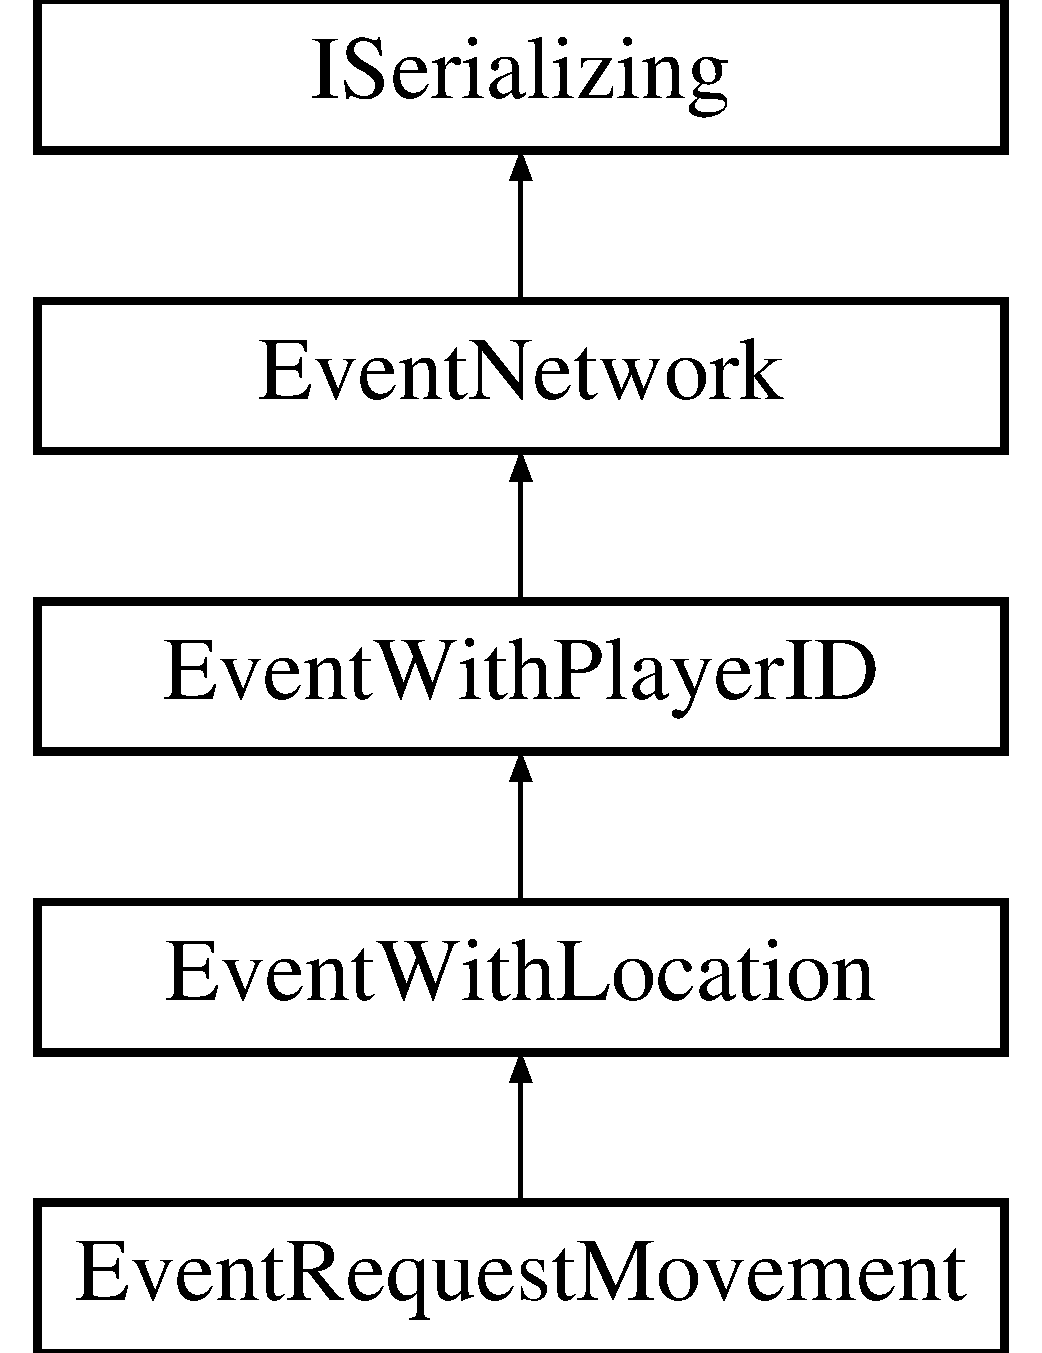
\includegraphics[height=5.000000cm]{class_event_request_movement}
\end{center}
\end{figure}
\subsection*{Public Member Functions}
\begin{DoxyCompactItemize}
\item 
\hypertarget{class_event_request_movement_ac23cc3d2b652f582980b751ec41aeb91}{{\bfseries Event\-Request\-Movement} (uint \hyperlink{class_event_with_i_d_a4b58cdaef622cb06405b6829a160cef5}{client\-I\-D}, uint \hyperlink{class_event_with_player_i_d_a41340c3a625e17bb56c31cc937db338e}{player\-I\-D}, float pos\-X, float pos\-Y, float vel\-X, float vel\-Y)}\label{class_event_request_movement_ac23cc3d2b652f582980b751ec41aeb91}

\item 
\hypertarget{class_event_request_movement_a67f08827339e593a94b9c3c183af89cf}{override int {\bfseries Get\-Size} ()}\label{class_event_request_movement_a67f08827339e593a94b9c3c183af89cf}

\item 
\hypertarget{class_event_request_movement_a43b5a9fa68ad25626bb08cf5dbb13d6c}{override void {\bfseries Serialize} (ref byte\mbox{[}$\,$\mbox{]} data, ref int last\-Index)}\label{class_event_request_movement_a43b5a9fa68ad25626bb08cf5dbb13d6c}

\end{DoxyCompactItemize}
\subsection*{Additional Inherited Members}


\subsection{Detailed Description}
Some player's character needs to be updated Client-\/$>$Server\-: Request the user update a certain players physics 

The documentation for this class was generated from the following file\-:\begin{DoxyCompactItemize}
\item 
/home/travis/build/temportalflux/\-Champ\-Net/\-Unity/\-Assets/\-Scripts/\-Network/events/Event\-Request\-Movement.\-cs\end{DoxyCompactItemize}

\hypertarget{class_event_with_location}{\section{Event\-With\-Location Class Reference}
\label{class_event_with_location}\index{Event\-With\-Location@{Event\-With\-Location}}
}
Inheritance diagram for Event\-With\-Location\-:\begin{figure}[H]
\begin{center}
\leavevmode
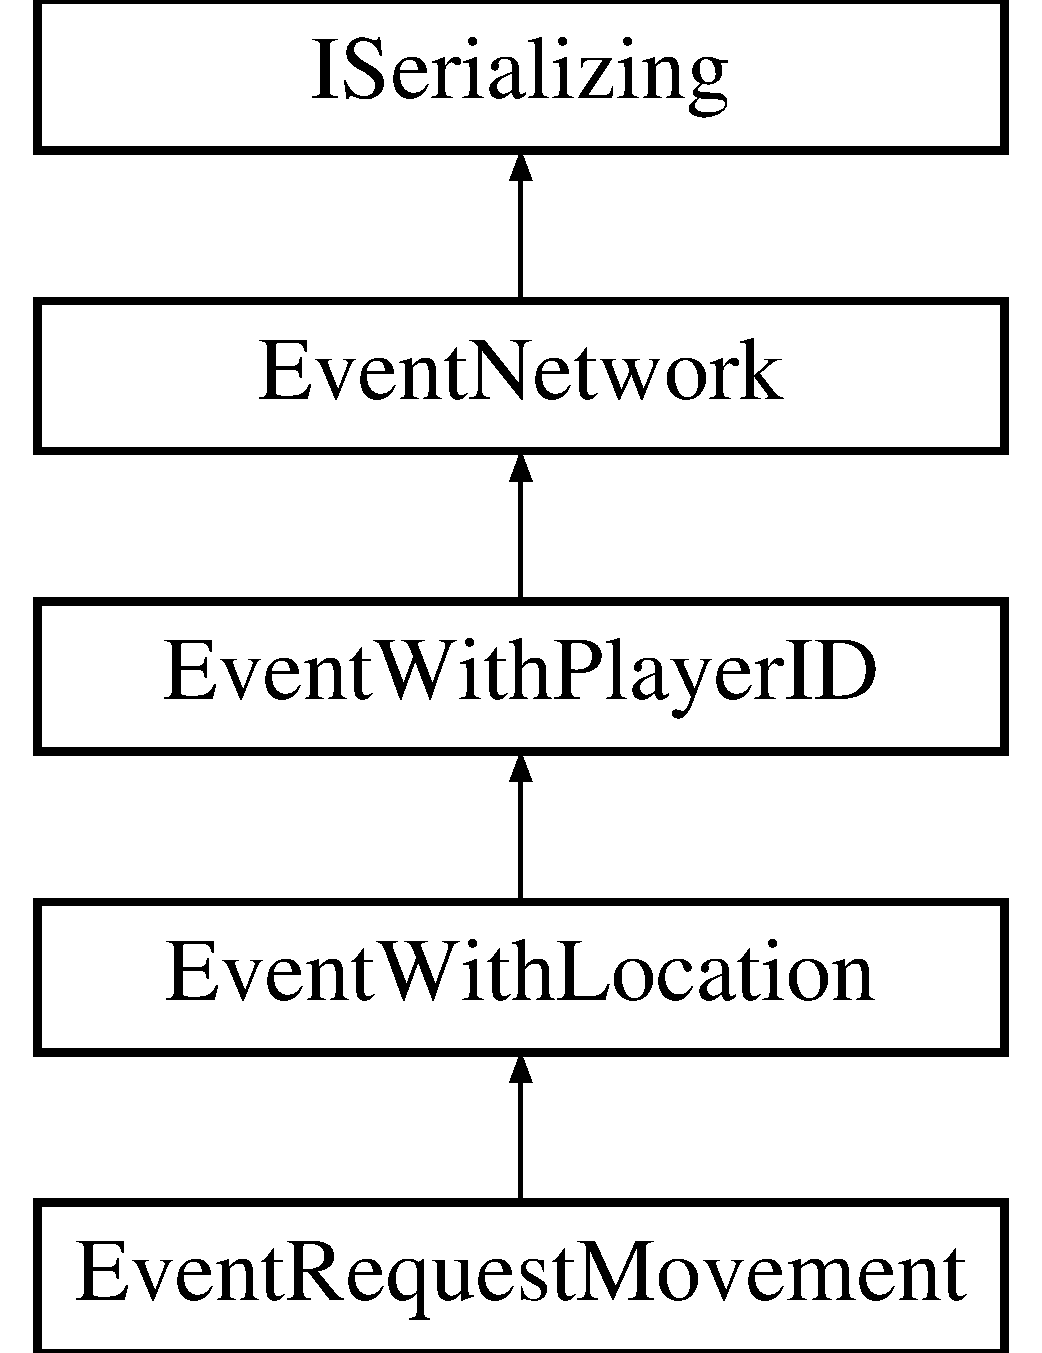
\includegraphics[height=5.000000cm]{class_event_with_location}
\end{center}
\end{figure}
\subsection*{Public Member Functions}
\begin{DoxyCompactItemize}
\item 
\hypertarget{class_event_with_location_a1771f2cfe61d2fe0e5c2e9c3918f1af0}{{\bfseries Event\-With\-Location} (byte id)}\label{class_event_with_location_a1771f2cfe61d2fe0e5c2e9c3918f1af0}

\end{DoxyCompactItemize}
\subsection*{Public Attributes}
\begin{DoxyCompactItemize}
\item 
\hypertarget{class_event_with_location_a60216348b1c3955d7d1365aaffa80f4f}{float {\bfseries pos\-X}}\label{class_event_with_location_a60216348b1c3955d7d1365aaffa80f4f}

\item 
\hypertarget{class_event_with_location_abcb12fbeee8ae457db23ab2e0aacd870}{float {\bfseries pos\-Y}}\label{class_event_with_location_abcb12fbeee8ae457db23ab2e0aacd870}

\end{DoxyCompactItemize}
\subsection*{Additional Inherited Members}


\subsection{Detailed Description}
A base event to (de)serialize a (float,float) location 

The documentation for this class was generated from the following file\-:\begin{DoxyCompactItemize}
\item 
/home/travis/build/temportalflux/\-Champ\-Net/\-Unity/\-Assets/\-Scripts/\-Network/events/Event\-With\-Location.\-cs\end{DoxyCompactItemize}

\hypertarget{class_event_with_player_i_d}{\section{Event\-With\-Player\-I\-D Class Reference}
\label{class_event_with_player_i_d}\index{Event\-With\-Player\-I\-D@{Event\-With\-Player\-I\-D}}
}
Inheritance diagram for Event\-With\-Player\-I\-D\-:\begin{figure}[H]
\begin{center}
\leavevmode
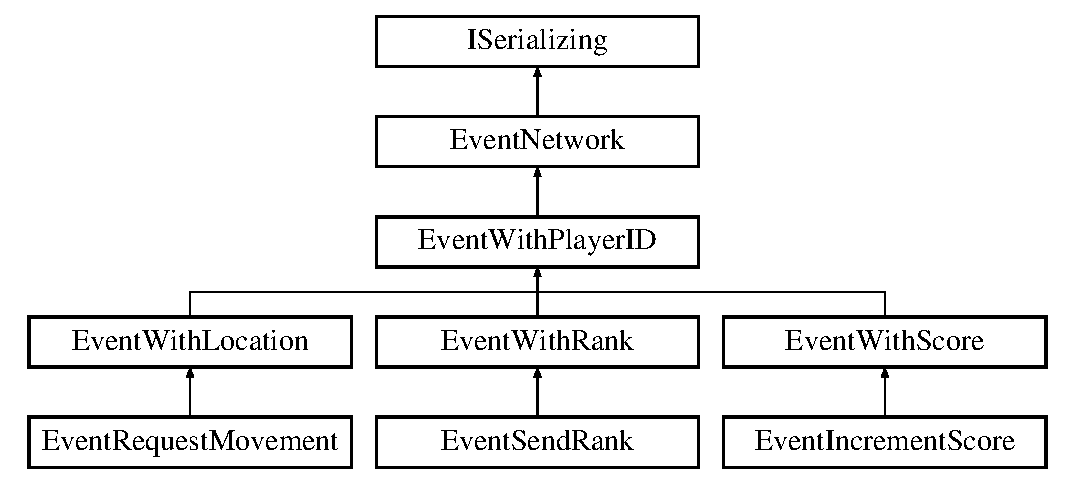
\includegraphics[height=4.545455cm]{class_event_with_player_i_d}
\end{center}
\end{figure}
\subsection*{Public Member Functions}
\begin{DoxyCompactItemize}
\item 
\hypertarget{class_event_with_player_i_d_a44a3302e35cd05c5501f6e6056be55ea}{{\bfseries Event\-With\-Player\-I\-D} (byte id)}\label{class_event_with_player_i_d_a44a3302e35cd05c5501f6e6056be55ea}

\item 
override int \hyperlink{class_event_with_player_i_d_a85e4b721aa1481d394d4c520d0103e74}{Get\-Size} ()
\begin{DoxyCompactList}\small\item\em Returns the size of the packet (the size for a potential byte\mbox{[}\mbox{]}) \end{DoxyCompactList}\item 
override void \hyperlink{class_event_with_player_i_d_a2492f5877e206df522bf181b10d2aeda}{Deserialize} (byte\mbox{[}$\,$\mbox{]} data, ref int last\-Index)
\begin{DoxyCompactList}\small\item\em Deserializes data from a byte array into this event's data \end{DoxyCompactList}\item 
override void \hyperlink{class_event_with_player_i_d_a3decca39195fe4e2fda1f8d57ca35a5f}{Serialize} (ref byte\mbox{[}$\,$\mbox{]} data, ref int last\-Index)
\begin{DoxyCompactList}\small\item\em Serializes data from this event into a byte array \end{DoxyCompactList}\end{DoxyCompactItemize}
\subsection*{Protected Attributes}
\begin{DoxyCompactItemize}
\item 
uint \hyperlink{class_event_with_player_i_d_a41340c3a625e17bb56c31cc937db338e}{player\-I\-D}
\begin{DoxyCompactList}\small\item\em The player identifier \end{DoxyCompactList}\end{DoxyCompactItemize}


\subsection{Member Function Documentation}
\hypertarget{class_event_with_player_i_d_a2492f5877e206df522bf181b10d2aeda}{\index{Event\-With\-Player\-I\-D@{Event\-With\-Player\-I\-D}!Deserialize@{Deserialize}}
\index{Deserialize@{Deserialize}!EventWithPlayerID@{Event\-With\-Player\-I\-D}}
\subsubsection[{Deserialize}]{\setlength{\rightskip}{0pt plus 5cm}override void Event\-With\-Player\-I\-D.\-Deserialize (
\begin{DoxyParamCaption}
\item[{byte\mbox{[}$\,$\mbox{]}}]{data, }
\item[{ref int}]{last\-Index}
\end{DoxyParamCaption}
)\hspace{0.3cm}{\ttfamily [inline]}}}\label{class_event_with_player_i_d_a2492f5877e206df522bf181b10d2aeda}


Deserializes data from a byte array into this event's data 


\begin{DoxyParams}{Parameters}
{\em data} & The data.\\
\hline
{\em last\-Index} & The last index.\\
\hline
\end{DoxyParams}


Author\-: Dustin Yost \hypertarget{class_event_with_player_i_d_a85e4b721aa1481d394d4c520d0103e74}{\index{Event\-With\-Player\-I\-D@{Event\-With\-Player\-I\-D}!Get\-Size@{Get\-Size}}
\index{Get\-Size@{Get\-Size}!EventWithPlayerID@{Event\-With\-Player\-I\-D}}
\subsubsection[{Get\-Size}]{\setlength{\rightskip}{0pt plus 5cm}override int Event\-With\-Player\-I\-D.\-Get\-Size (
\begin{DoxyParamCaption}
{}
\end{DoxyParamCaption}
)\hspace{0.3cm}{\ttfamily [inline]}}}\label{class_event_with_player_i_d_a85e4b721aa1481d394d4c520d0103e74}


Returns the size of the packet (the size for a potential byte\mbox{[}\mbox{]}) 

\begin{DoxyReturn}{Returns}
the integer length of a byte array to hold this event's data 
\end{DoxyReturn}


Author\-: Dustin Yost \hypertarget{class_event_with_player_i_d_a3decca39195fe4e2fda1f8d57ca35a5f}{\index{Event\-With\-Player\-I\-D@{Event\-With\-Player\-I\-D}!Serialize@{Serialize}}
\index{Serialize@{Serialize}!EventWithPlayerID@{Event\-With\-Player\-I\-D}}
\subsubsection[{Serialize}]{\setlength{\rightskip}{0pt plus 5cm}override void Event\-With\-Player\-I\-D.\-Serialize (
\begin{DoxyParamCaption}
\item[{ref byte\mbox{[}$\,$\mbox{]}}]{data, }
\item[{ref int}]{last\-Index}
\end{DoxyParamCaption}
)\hspace{0.3cm}{\ttfamily [inline]}}}\label{class_event_with_player_i_d_a3decca39195fe4e2fda1f8d57ca35a5f}


Serializes data from this event into a byte array 


\begin{DoxyParams}{Parameters}
{\em data} & The data.\\
\hline
{\em last\-Index} & The last index.\\
\hline
\end{DoxyParams}


Author\-: Dustin Yost 

\subsection{Member Data Documentation}
\hypertarget{class_event_with_player_i_d_a41340c3a625e17bb56c31cc937db338e}{\index{Event\-With\-Player\-I\-D@{Event\-With\-Player\-I\-D}!player\-I\-D@{player\-I\-D}}
\index{player\-I\-D@{player\-I\-D}!EventWithPlayerID@{Event\-With\-Player\-I\-D}}
\subsubsection[{player\-I\-D}]{\setlength{\rightskip}{0pt plus 5cm}uint Event\-With\-Player\-I\-D.\-player\-I\-D\hspace{0.3cm}{\ttfamily [protected]}}}\label{class_event_with_player_i_d_a41340c3a625e17bb56c31cc937db338e}


The player identifier 



The documentation for this class was generated from the following file\-:\begin{DoxyCompactItemize}
\item 
/home/travis/build/temportalflux/\-Champ\-Net/\-Unity/\-Assets/\-Scripts/\-Network/events/Event\-With\-Player\-I\-D.\-cs\end{DoxyCompactItemize}

\hypertarget{class_game}{\section{Game Class Reference}
\label{class_game}\index{Game@{Game}}
}


{\ttfamily \#include $<$Game.\-h$>$}

\subsection*{Public Member Functions}
\begin{DoxyCompactItemize}
\item 
\hyperlink{class_game_a09f1b8c714816ee634939b73fe08622d}{Game} (\hyperlink{class_state_application}{State\-Application} $\ast$state)
\item 
\hypertarget{class_game_aa61c0358c2611d00eb47ebf72a88f8c7}{const bool {\bfseries is\-Running} () const }\label{class_game_aa61c0358c2611d00eb47ebf72a88f8c7}

\item 
\hypertarget{class_game_ac405429a34ce63322174063442040259}{\hyperlink{struct_state_data}{State\-Data} $\ast$ {\bfseries get\-Data} () const }\label{class_game_ac405429a34ce63322174063442040259}

\item 
void \hyperlink{class_game_a79df6376b332d63c9eca0dcee30305c3}{update} ()
\item 
\hypertarget{class_game_afe06acbc24125f9a7e9d94f7740315fb}{void {\bfseries queue\-State} (\hyperlink{class_state_application}{State\-Application} $\ast$next\-State)}\label{class_game_afe06acbc24125f9a7e9d94f7740315fb}

\item 
\hypertarget{class_game_afa29034b42f2825221ffea4fac919363}{void {\bfseries go\-To\-Next\-State} ()}\label{class_game_afa29034b42f2825221ffea4fac919363}

\end{DoxyCompactItemize}
\subsection*{Static Public Attributes}
\begin{DoxyCompactItemize}
\item 
\hypertarget{class_game_a9518d0c89b6d47d2e3042809bc9c5f6a}{static \hyperlink{class_game}{Game} $\ast$ {\bfseries gp\-Game} = N\-U\-L\-L}\label{class_game_a9518d0c89b6d47d2e3042809bc9c5f6a}

\end{DoxyCompactItemize}
\subsection*{Protected Attributes}
\begin{DoxyCompactItemize}
\item 
\hypertarget{class_game_a1f85e8206f06c0bd64430effae32c577}{\hyperlink{class_state_application}{State\-Application} $\ast$ {\bfseries mp\-State}}\label{class_game_a1f85e8206f06c0bd64430effae32c577}

\item 
\hypertarget{class_game_aaa55cde79b9892b0a364b9a165ca942e}{\hyperlink{class_state_application}{State\-Application} $\ast$ {\bfseries mp\-Next}}\label{class_game_aaa55cde79b9892b0a364b9a165ca942e}

\end{DoxyCompactItemize}


\subsection{Detailed Description}
Author\-: Dustin Yost A base class for all update loop based game information (runs the game) 

\subsection{Constructor \& Destructor Documentation}
\hypertarget{class_game_a09f1b8c714816ee634939b73fe08622d}{\index{Game@{Game}!Game@{Game}}
\index{Game@{Game}!Game@{Game}}
\subsubsection[{Game}]{\setlength{\rightskip}{0pt plus 5cm}Game\-::\-Game (
\begin{DoxyParamCaption}
\item[{{\bf State\-Application} $\ast$}]{state}
\end{DoxyParamCaption}
)}}\label{class_game_a09f1b8c714816ee634939b73fe08622d}
Author\-: Dustin Yost A base class for all update loop based game information (runs the game) 

\subsection{Member Function Documentation}
\hypertarget{class_game_a79df6376b332d63c9eca0dcee30305c3}{\index{Game@{Game}!update@{update}}
\index{update@{update}!Game@{Game}}
\subsubsection[{update}]{\setlength{\rightskip}{0pt plus 5cm}void Game\-::update (
\begin{DoxyParamCaption}
{}
\end{DoxyParamCaption}
)}}\label{class_game_a79df6376b332d63c9eca0dcee30305c3}
Author\-: Dustin Yost Handles all gameloop updates 

The documentation for this class was generated from the following files\-:\begin{DoxyCompactItemize}
\item 
/home/travis/build/temportalflux/\-Champ\-Net/\-Champ\-Net/\-Champ\-Net\-Plugin\-Test/include/Game.\-h\item 
/home/travis/build/temportalflux/\-Champ\-Net/\-Champ\-Net/\-Champ\-Net\-Plugin\-Test/source/Game.\-cpp\end{DoxyCompactItemize}

\hypertarget{class_game_manager_1_1_game_action}{\section{Game\-Manager.\-Game\-Action Class Reference}
\label{class_game_manager_1_1_game_action}\index{Game\-Manager.\-Game\-Action@{Game\-Manager.\-Game\-Action}}
}
Inheritance diagram for Game\-Manager.\-Game\-Action\-:\begin{figure}[H]
\begin{center}
\leavevmode
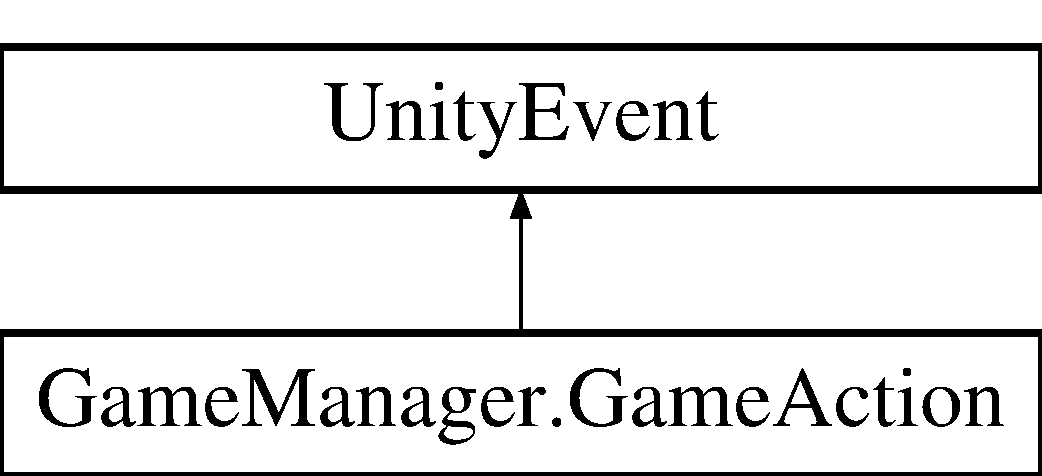
\includegraphics[height=2.000000cm]{class_game_manager_1_1_game_action}
\end{center}
\end{figure}


The documentation for this class was generated from the following file\-:\begin{DoxyCompactItemize}
\item 
/home/travis/build/temportalflux/\-Champ\-Net/\-Unity/\-Assets/\-Scripts/Game\-Manager.\-cs\end{DoxyCompactItemize}

\hypertarget{class_game_manager_1_1_game_action_flag}{\section{Game\-Manager.\-Game\-Action\-Flag Class Reference}
\label{class_game_manager_1_1_game_action_flag}\index{Game\-Manager.\-Game\-Action\-Flag@{Game\-Manager.\-Game\-Action\-Flag}}
}
Inheritance diagram for Game\-Manager.\-Game\-Action\-Flag\-:\begin{figure}[H]
\begin{center}
\leavevmode
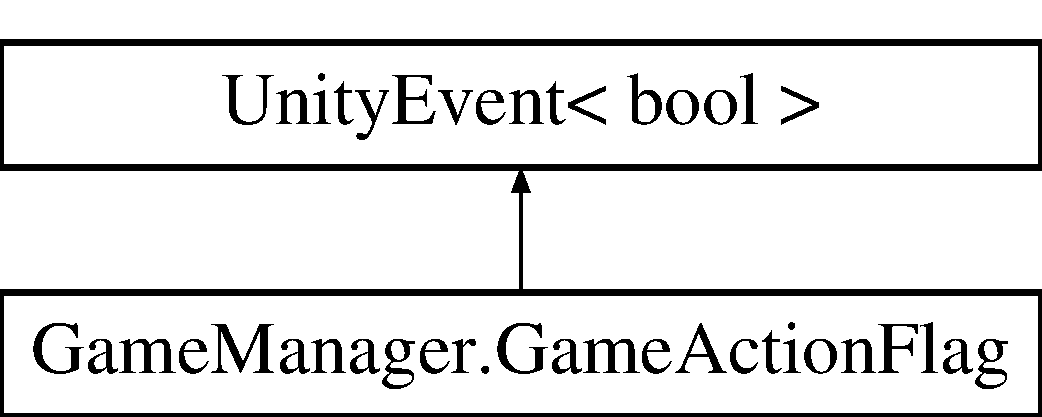
\includegraphics[height=2.000000cm]{class_game_manager_1_1_game_action_flag}
\end{center}
\end{figure}


The documentation for this class was generated from the following file\-:\begin{DoxyCompactItemize}
\item 
/home/travis/build/temportalflux/\-Champ\-Net/\-Unity/\-Assets/\-Scripts/Game\-Manager.\-cs\end{DoxyCompactItemize}

\hypertarget{class_game_manager_1_1_game_action_message}{\section{Game\-Manager.\-Game\-Action\-Message Class Reference}
\label{class_game_manager_1_1_game_action_message}\index{Game\-Manager.\-Game\-Action\-Message@{Game\-Manager.\-Game\-Action\-Message}}
}
Inheritance diagram for Game\-Manager.\-Game\-Action\-Message\-:\begin{figure}[H]
\begin{center}
\leavevmode
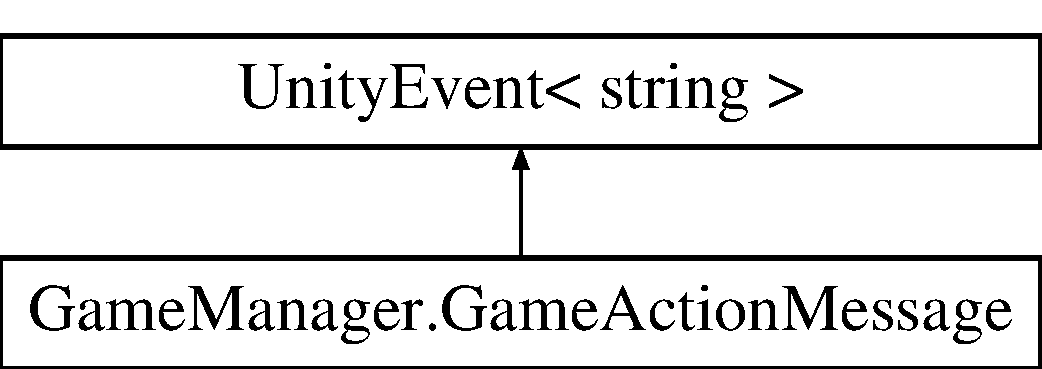
\includegraphics[height=2.000000cm]{class_game_manager_1_1_game_action_message}
\end{center}
\end{figure}


The documentation for this class was generated from the following file\-:\begin{DoxyCompactItemize}
\item 
/home/travis/build/temportalflux/\-Champ\-Net/\-Unity/\-Assets/\-Scripts/Game\-Manager.\-cs\end{DoxyCompactItemize}

\hypertarget{class_game_manager}{\section{Game\-Manager Class Reference}
\label{class_game_manager}\index{Game\-Manager@{Game\-Manager}}
}


The manager for the client game Is a singleton, instatiated in the first scene  


Inheritance diagram for Game\-Manager\-:\begin{figure}[H]
\begin{center}
\leavevmode
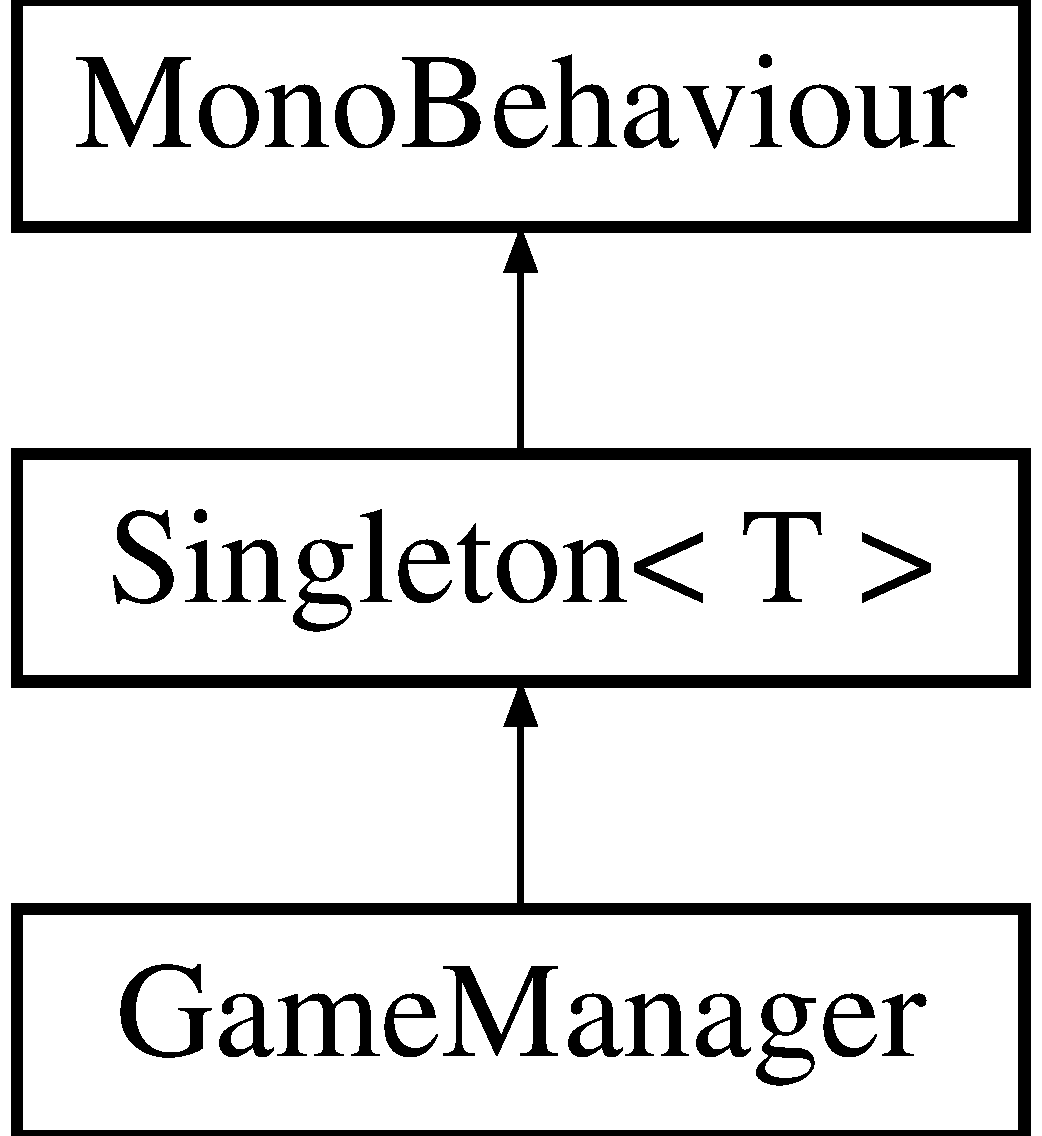
\includegraphics[height=3.000000cm]{class_game_manager}
\end{center}
\end{figure}
\subsection*{Classes}
\begin{DoxyCompactItemize}
\item 
class \hyperlink{class_game_manager_1_1_game_action}{Game\-Action}
\item 
class \hyperlink{class_game_manager_1_1_game_action_flag}{Game\-Action\-Flag}
\item 
class \hyperlink{class_game_manager_1_1_game_action_message}{Game\-Action\-Message}
\end{DoxyCompactItemize}
\subsection*{Public Member Functions}
\begin{DoxyCompactItemize}
\item 
void \hyperlink{class_game_manager_a3403831c40f16191e3997be60d95380b}{Play} ()
\begin{DoxyCompactList}\small\item\em Start the game in a local world \end{DoxyCompactList}\item 
void \hyperlink{class_game_manager_a1138f86278583414cba9456d02d0fa1c}{Play\-Network} ()
\begin{DoxyCompactList}\small\item\em Start the game in a networked world \end{DoxyCompactList}\item 
void \hyperlink{class_game_manager_a3c3a8e05664851d7642c13989af691cf}{Network\-Connect} (string address, int port, Connect\-Menu.\-Player\-Descriptor\mbox{[}$\,$\mbox{]} players)
\begin{DoxyCompactList}\small\item\em Connect the client with some server \end{DoxyCompactList}\item 
void \hyperlink{class_game_manager_a5d9cafdd495a4ed2760de13b7b9c80b6}{Exit} ()
\begin{DoxyCompactList}\small\item\em Exit the current scene \end{DoxyCompactList}\item 
\hyperlink{class_player_reference}{Player\-Reference} \hyperlink{class_game_manager_aadd5e389068b81b09036cc2bb8c097d6}{get\-Random\-Player} (\hyperlink{class_game_state_1_1_player}{Game\-State.\-Player} not\-Me)
\begin{DoxyCompactList}\small\item\em Get a random player from the current player listings in Game\-State.\-players \end{DoxyCompactList}\item 
Audio\-Source \hyperlink{class_game_manager_abf59d5ce551af5e35529f71a99d89d76}{Get\-Music\-Source} ()
\begin{DoxyCompactList}\small\item\em Gets the music source. \end{DoxyCompactList}\item 
\hypertarget{class_game_manager_a414dcfd0d1f5a5904d2440165e42923d}{void {\bfseries grab\-Score\-Board} ()}\label{class_game_manager_a414dcfd0d1f5a5904d2440165e42923d}

\item 
\hypertarget{class_game_manager_a9d3b6a3fb49a9402e1afde9224a12e21}{void {\bfseries Load\-Battle\-Scene} (\hyperlink{class_battle_participant}{Battle\-Participant} p1, \hyperlink{class_battle_participant}{Battle\-Participant} p2, bool is\-Netwoked\-Battle)}\label{class_game_manager_a9d3b6a3fb49a9402e1afde9224a12e21}

\item 
\hypertarget{class_game_manager_a4b49768a7f34b0f3795741f997eca643}{void {\bfseries Unload\-Battle\-Scene} ()}\label{class_game_manager_a4b49768a7f34b0f3795741f997eca643}

\end{DoxyCompactItemize}
\subsection*{Public Attributes}
\begin{DoxyCompactItemize}
\item 
\hypertarget{class_game_manager_a87d481fe88a1765f436ea5764cd1a21a}{\hyperlink{class_game_manager_1_1_game_action_flag}{Game\-Action\-Flag} {\bfseries on\-Network\-Connection\-Handled}}\label{class_game_manager_a87d481fe88a1765f436ea5764cd1a21a}

\item 
\hypertarget{class_game_manager_af977df043b83671ab9a4753b90fbf75b}{\hyperlink{class_game_manager_1_1_game_action_message}{Game\-Action\-Message} {\bfseries on\-Network\-Rejected}}\label{class_game_manager_af977df043b83671ab9a4753b90fbf75b}

\item 
\hyperlink{class_scene_transition}{Scene\-Transition} \hyperlink{class_game_manager_abae15982d4eb90ef9e5f3d24d15e22f2}{transition}
\begin{DoxyCompactList}\small\item\em The object to handle transitioning between scenes \end{DoxyCompactList}\item 
\hypertarget{class_game_manager_a57d400c7a28f42865048fbdbaf236cfb}{Game\-Object {\bfseries player\-Prefab}}\label{class_game_manager_a57d400c7a28f42865048fbdbaf236cfb}

\item 
\hyperlink{class_game_state}{Game\-State} \hyperlink{class_game_manager_a8d86b330237462e38933b28276ed0e2c}{state}
\begin{DoxyCompactList}\small\item\em The game state \end{DoxyCompactList}\item 
Main\-Camera \hyperlink{class_game_manager_aafd6b83529911d9e32cc4b79bd477d74}{main\-Camera}
\begin{DoxyCompactList}\small\item\em The main camera in the open-\/world \end{DoxyCompactList}\end{DoxyCompactItemize}
\subsection*{Properties}
\begin{DoxyCompactItemize}
\item 
static \hyperlink{class_game_manager}{Game\-Manager} \hyperlink{class_game_manager_a5c1d1f77dd4a2668a47a75c934c87075}{I\-N\-S\-T\-A\-N\-C\-E}\hspace{0.3cm}{\ttfamily  \mbox{[}get\mbox{]}}
\begin{DoxyCompactList}\small\item\em The public getter for the instance \end{DoxyCompactList}\end{DoxyCompactItemize}
\subsection*{Additional Inherited Members}


\subsection{Detailed Description}
The manager for the client game Is a singleton, instatiated in the first scene 

$<$author$>$Dustin Yost$<$/author$>$ 

\subsection{Member Function Documentation}
\hypertarget{class_game_manager_a5d9cafdd495a4ed2760de13b7b9c80b6}{\index{Game\-Manager@{Game\-Manager}!Exit@{Exit}}
\index{Exit@{Exit}!GameManager@{Game\-Manager}}
\subsubsection[{Exit}]{\setlength{\rightskip}{0pt plus 5cm}void Game\-Manager.\-Exit (
\begin{DoxyParamCaption}
{}
\end{DoxyParamCaption}
)\hspace{0.3cm}{\ttfamily [inline]}}}\label{class_game_manager_a5d9cafdd495a4ed2760de13b7b9c80b6}


Exit the current scene 

\hypertarget{class_game_manager_abf59d5ce551af5e35529f71a99d89d76}{\index{Game\-Manager@{Game\-Manager}!Get\-Music\-Source@{Get\-Music\-Source}}
\index{Get\-Music\-Source@{Get\-Music\-Source}!GameManager@{Game\-Manager}}
\subsubsection[{Get\-Music\-Source}]{\setlength{\rightskip}{0pt plus 5cm}Audio\-Source Game\-Manager.\-Get\-Music\-Source (
\begin{DoxyParamCaption}
{}
\end{DoxyParamCaption}
)\hspace{0.3cm}{\ttfamily [inline]}}}\label{class_game_manager_abf59d5ce551af5e35529f71a99d89d76}


Gets the music source. 

\begin{DoxyReturn}{Returns}
The Audio\-Source component
\end{DoxyReturn}
\hypertarget{class_game_manager_aadd5e389068b81b09036cc2bb8c097d6}{\index{Game\-Manager@{Game\-Manager}!get\-Random\-Player@{get\-Random\-Player}}
\index{get\-Random\-Player@{get\-Random\-Player}!GameManager@{Game\-Manager}}
\subsubsection[{get\-Random\-Player}]{\setlength{\rightskip}{0pt plus 5cm}{\bf Player\-Reference} Game\-Manager.\-get\-Random\-Player (
\begin{DoxyParamCaption}
\item[{{\bf Game\-State.\-Player}}]{not\-Me}
\end{DoxyParamCaption}
)\hspace{0.3cm}{\ttfamily [inline]}}}\label{class_game_manager_aadd5e389068b81b09036cc2bb8c097d6}


Get a random player from the current player listings in Game\-State.\-players 


\begin{DoxyParams}{Parameters}
{\em not\-Me} & The player which should not be included\\
\hline
\end{DoxyParams}
\begin{DoxyReturn}{Returns}

\end{DoxyReturn}
\hypertarget{class_game_manager_a3c3a8e05664851d7642c13989af691cf}{\index{Game\-Manager@{Game\-Manager}!Network\-Connect@{Network\-Connect}}
\index{Network\-Connect@{Network\-Connect}!GameManager@{Game\-Manager}}
\subsubsection[{Network\-Connect}]{\setlength{\rightskip}{0pt plus 5cm}void Game\-Manager.\-Network\-Connect (
\begin{DoxyParamCaption}
\item[{string}]{address, }
\item[{int}]{port, }
\item[{Connect\-Menu.\-Player\-Descriptor\mbox{[}$\,$\mbox{]}}]{players}
\end{DoxyParamCaption}
)\hspace{0.3cm}{\ttfamily [inline]}}}\label{class_game_manager_a3c3a8e05664851d7642c13989af691cf}


Connect the client with some server 


\begin{DoxyParams}{Parameters}
{\em address} & The I\-Pv4 address\\
\hline
{\em port} & The address port\\
\hline
{\em players} & the desired player descriptors to connect with\\
\hline
\end{DoxyParams}
\hypertarget{class_game_manager_a3403831c40f16191e3997be60d95380b}{\index{Game\-Manager@{Game\-Manager}!Play@{Play}}
\index{Play@{Play}!GameManager@{Game\-Manager}}
\subsubsection[{Play}]{\setlength{\rightskip}{0pt plus 5cm}void Game\-Manager.\-Play (
\begin{DoxyParamCaption}
{}
\end{DoxyParamCaption}
)\hspace{0.3cm}{\ttfamily [inline]}}}\label{class_game_manager_a3403831c40f16191e3997be60d95380b}


Start the game in a local world 

\hypertarget{class_game_manager_a1138f86278583414cba9456d02d0fa1c}{\index{Game\-Manager@{Game\-Manager}!Play\-Network@{Play\-Network}}
\index{Play\-Network@{Play\-Network}!GameManager@{Game\-Manager}}
\subsubsection[{Play\-Network}]{\setlength{\rightskip}{0pt plus 5cm}void Game\-Manager.\-Play\-Network (
\begin{DoxyParamCaption}
{}
\end{DoxyParamCaption}
)\hspace{0.3cm}{\ttfamily [inline]}}}\label{class_game_manager_a1138f86278583414cba9456d02d0fa1c}


Start the game in a networked world 



\subsection{Member Data Documentation}
\hypertarget{class_game_manager_aafd6b83529911d9e32cc4b79bd477d74}{\index{Game\-Manager@{Game\-Manager}!main\-Camera@{main\-Camera}}
\index{main\-Camera@{main\-Camera}!GameManager@{Game\-Manager}}
\subsubsection[{main\-Camera}]{\setlength{\rightskip}{0pt plus 5cm}Main\-Camera Game\-Manager.\-main\-Camera}}\label{class_game_manager_aafd6b83529911d9e32cc4b79bd477d74}


The main camera in the open-\/world 

\hypertarget{class_game_manager_a8d86b330237462e38933b28276ed0e2c}{\index{Game\-Manager@{Game\-Manager}!state@{state}}
\index{state@{state}!GameManager@{Game\-Manager}}
\subsubsection[{state}]{\setlength{\rightskip}{0pt plus 5cm}{\bf Game\-State} Game\-Manager.\-state}}\label{class_game_manager_a8d86b330237462e38933b28276ed0e2c}


The game state 

\hypertarget{class_game_manager_abae15982d4eb90ef9e5f3d24d15e22f2}{\index{Game\-Manager@{Game\-Manager}!transition@{transition}}
\index{transition@{transition}!GameManager@{Game\-Manager}}
\subsubsection[{transition}]{\setlength{\rightskip}{0pt plus 5cm}{\bf Scene\-Transition} Game\-Manager.\-transition}}\label{class_game_manager_abae15982d4eb90ef9e5f3d24d15e22f2}


The object to handle transitioning between scenes 



\subsection{Property Documentation}
\hypertarget{class_game_manager_a5c1d1f77dd4a2668a47a75c934c87075}{\index{Game\-Manager@{Game\-Manager}!I\-N\-S\-T\-A\-N\-C\-E@{I\-N\-S\-T\-A\-N\-C\-E}}
\index{I\-N\-S\-T\-A\-N\-C\-E@{I\-N\-S\-T\-A\-N\-C\-E}!GameManager@{Game\-Manager}}
\subsubsection[{I\-N\-S\-T\-A\-N\-C\-E}]{\setlength{\rightskip}{0pt plus 5cm}{\bf Game\-Manager} Game\-Manager.\-I\-N\-S\-T\-A\-N\-C\-E\hspace{0.3cm}{\ttfamily [static]}, {\ttfamily [get]}}}\label{class_game_manager_a5c1d1f77dd4a2668a47a75c934c87075}


The public getter for the instance 



The documentation for this class was generated from the following file\-:\begin{DoxyCompactItemize}
\item 
/home/travis/build/temportalflux/\-Champ\-Net/\-Unity/\-Assets/\-Scripts/Game\-Manager.\-cs\end{DoxyCompactItemize}

\hypertarget{class_game_state}{\section{Game\-State Class Reference}
\label{class_game_state}\index{Game\-State@{Game\-State}}
}


Holds all persistent data from network intergration for local usage  


Inheritance diagram for Game\-State\-:\begin{figure}[H]
\begin{center}
\leavevmode
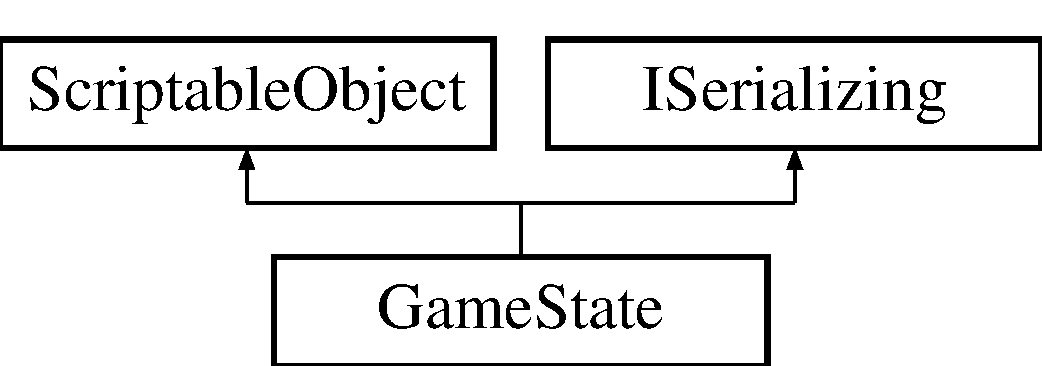
\includegraphics[height=2.000000cm]{class_game_state}
\end{center}
\end{figure}
\subsection*{Classes}
\begin{DoxyCompactItemize}
\item 
struct \hyperlink{class_game_state_1_1_player}{Player}
\begin{DoxyCompactList}\small\item\em A state class for all \hyperlink{class_game_state_1_1_player}{Player} objects \end{DoxyCompactList}\end{DoxyCompactItemize}
\subsection*{Public Member Functions}
\begin{DoxyCompactItemize}
\item 
\hypertarget{class_game_state_a05acc40696378ba026165a2cc824acf0}{bool {\bfseries Has\-Player} (ref \hyperlink{class_game_state_1_1_player}{Player} info)}\label{class_game_state_a05acc40696378ba026165a2cc824acf0}

\item 
void \hyperlink{class_game_state_a4c4e32237639764263332c7c236974d1}{Add\-Player} (\hyperlink{class_game_state_1_1_player}{Player} info)
\begin{DoxyCompactList}\small\item\em Add a player to the current game object scene via its info \end{DoxyCompactList}\item 
\hypertarget{class_game_state_ae8d21ce826daada0dabeadd11c6eb233}{void {\bfseries Remove\-Player} (\hyperlink{class_game_state_1_1_player}{Player} info)}\label{class_game_state_ae8d21ce826daada0dabeadd11c6eb233}

\item 
\hypertarget{class_game_state_a1e3c3340e55693af1c8326879a81f1c4}{void {\bfseries Add\-Player\-Local} (\hyperlink{class_game_state_1_1_player}{Player} info)}\label{class_game_state_a1e3c3340e55693af1c8326879a81f1c4}

\item 
\hypertarget{class_game_state_a2e6cdef311e93ec46d07206d621f6837}{void {\bfseries Add\-Player\-Connected} (\hyperlink{class_game_state_1_1_player}{Player} info)}\label{class_game_state_a2e6cdef311e93ec46d07206d621f6837}

\item 
\hypertarget{class_game_state_a61e4817740bd283ce4a6ea44e0d0f00a}{void {\bfseries Spawn\-Local\-Multiplayer} ()}\label{class_game_state_a61e4817740bd283ce4a6ea44e0d0f00a}

\item 
\hypertarget{class_game_state_a82b88c45043a403441d3eef1e0b72266}{void {\bfseries Spawn\-Local\-Player} ()}\label{class_game_state_a82b88c45043a403441d3eef1e0b72266}

\item 
\hypertarget{class_game_state_af2fbb55979f8cc6da50317e1d701e370}{void {\bfseries Spawn\-Player} ()}\label{class_game_state_af2fbb55979f8cc6da50317e1d701e370}

\item 
int \hyperlink{class_game_state_a57d152b243c11aa86e7ba0f07b4bd0dd}{Get\-Size} ()
\begin{DoxyCompactList}\small\item\em Returns the size of the packet (the size for a potential byte\mbox{[}\mbox{]}) \end{DoxyCompactList}\item 
void \hyperlink{class_game_state_af57a06c77a763e8b57841bab79c9b12f}{Serialize} (ref byte\mbox{[}$\,$\mbox{]} data, ref int last\-Index)
\begin{DoxyCompactList}\small\item\em Serializes data from this event into a byte array. Unused for \hyperlink{class_game_state}{Game\-State}. Game\-States are O\-N\-L\-Y serialized via server. \end{DoxyCompactList}\item 
void \hyperlink{class_game_state_aa5f956de2c49182fbe5fc32e9d2ca431}{Deserialize} (byte\mbox{[}$\,$\mbox{]} data, ref int last\-Index)
\begin{DoxyCompactList}\small\item\em Deserializes data from a byte array into this event's data \end{DoxyCompactList}\item 
\hypertarget{class_game_state_a268b639f06e4fa7fa1ca1819cc5d3175}{void {\bfseries Fixed\-Update} ()}\label{class_game_state_a268b639f06e4fa7fa1ca1819cc5d3175}

\item 
\hypertarget{class_game_state_a74a35fb7045c0eee7e68f07c387e2ddf}{{\bfseries Game\-State} (int id)}\label{class_game_state_a74a35fb7045c0eee7e68f07c387e2ddf}

\item 
\hypertarget{class_game_state_ad74bf5767b052d5b32805220ca0c1fab}{void {\bfseries add\-Player} (unsigned int \hyperlink{class_game_state_ad24a423ba6655fc6541b2f12ce98e0d0}{client\-I\-D}, unsigned int player\-I\-D, unsigned int local\-I\-D, std\-::string name, float color\-R, float color\-G, float color\-B)}\label{class_game_state_ad74bf5767b052d5b32805220ca0c1fab}

\item 
\hypertarget{class_game_state_a733fa68895adba783b0b4b804f16906f}{void {\bfseries remove\-Player} (unsigned int player\-I\-D)}\label{class_game_state_a733fa68895adba783b0b4b804f16906f}

\item 
\hypertarget{class_game_state_a291fcda337b1a25c21871fe338399c27}{char $\ast$ {\bfseries serialize\-For\-Client} (unsigned char packet\-I\-D, int \hyperlink{class_game_state_ad24a423ba6655fc6541b2f12ce98e0d0}{client\-I\-D}, int \&data\-Length)}\label{class_game_state_a291fcda337b1a25c21871fe338399c27}

\end{DoxyCompactItemize}
\subsection*{Static Public Member Functions}
\begin{DoxyCompactItemize}
\item 
static void \hyperlink{class_game_state_a2f3154927e33e16bd595b4aece996c61}{Create} ()
\begin{DoxyCompactList}\small\item\em Creates a Scriptable\-Object for \hyperlink{class_game_state}{Game\-State} from a Unity Menu context \end{DoxyCompactList}\end{DoxyCompactItemize}
\subsection*{Public Attributes}
\begin{DoxyCompactItemize}
\item 
Connect\-Menu.\-Player\-Descriptor\mbox{[}$\,$\mbox{]} \hyperlink{class_game_state_a8b1949523ac8e40776c0617666023d64}{player\-Request} = null
\begin{DoxyCompactList}\small\item\em Not Serialized. Used to store the requests for players on world-\/enter \end{DoxyCompactList}\item 
\hypertarget{class_game_state_ad68ed3f1f32060bfff68d296e6750712}{bool {\bfseries editor\-Foldout\-Players}}\label{class_game_state_ad68ed3f1f32060bfff68d296e6750712}

\item 
\hypertarget{class_game_state_a47358e83d829da7a28c49f8d0a795125}{Dictionary$<$ I\-D, bool $>$ {\bfseries editor\-Foldouts}}\label{class_game_state_a47358e83d829da7a28c49f8d0a795125}

\item 
\hypertarget{class_game_state_aa4cba70bc38a13e80439dc784c6ca12e}{bool {\bfseries is\-Local\-Game}}\label{class_game_state_aa4cba70bc38a13e80439dc784c6ca12e}

\item 
uint \hyperlink{class_game_state_ad24a423ba6655fc6541b2f12ce98e0d0}{client\-I\-D}
\begin{DoxyCompactList}\small\item\em A unique identifier (across all peers in the network) of the client which controls this player \end{DoxyCompactList}\item 
\hypertarget{class_game_state_a3d88394849f2356b1c1917f8bb9cc873}{\hyperlink{class_monster_data_object}{Monster\-Data\-Object}\mbox{[}$\,$\mbox{]} {\bfseries starters}}\label{class_game_state_a3d88394849f2356b1c1917f8bb9cc873}

\item 
\hypertarget{class_game_state_a857eed8c97274c3dd9d3eb558a33f855}{float {\bfseries delta\-Time}}\label{class_game_state_a857eed8c97274c3dd9d3eb558a33f855}

\item 
\hypertarget{class_game_state_aed9c4cf83c497c6e36585e0ed3999564}{Dictionary$<$ I\-D, \hyperlink{class_game_state_1_1_player}{Player} $>$ {\bfseries players}}\label{class_game_state_aed9c4cf83c497c6e36585e0ed3999564}

\item 
\hypertarget{class_game_state_adb8c9c7f10d683332cbd62927d35cb35}{int {\bfseries client\-I\-D}}\label{class_game_state_adb8c9c7f10d683332cbd62927d35cb35}

\item 
\hypertarget{class_game_state_a8f156a6cce5f2b9945c274b6bfc971ce}{std\-::map$<$ unsigned int, \hyperlink{class_game_state_1_1_player}{Player} $>$ {\bfseries players}}\label{class_game_state_a8f156a6cce5f2b9945c274b6bfc971ce}

\end{DoxyCompactItemize}
\subsection*{Properties}
\begin{DoxyCompactItemize}
\item 
\hypertarget{class_game_state_a3fe38a9e11fe72dd4bc4796e1d4a6c1b}{Dictionary$<$ uint, \hyperlink{class_game_state_1_1_player}{Player} $>$ {\bfseries local\-Players}\hspace{0.3cm}{\ttfamily  \mbox{[}get\mbox{]}}}\label{class_game_state_a3fe38a9e11fe72dd4bc4796e1d4a6c1b}

\item 
\hypertarget{class_game_state_ad0f225ac26f38bf21be10d35a1cd6011}{Dictionary$<$ uint, \hyperlink{class_game_state_1_1_player}{Player} $>$ {\bfseries connected\-Players}\hspace{0.3cm}{\ttfamily  \mbox{[}get\mbox{]}}}\label{class_game_state_ad0f225ac26f38bf21be10d35a1cd6011}

\end{DoxyCompactItemize}


\subsection{Detailed Description}
Holds all persistent data from network intergration for local usage 

\begin{DoxyAuthor}{Author}
Dustin Yost 
\end{DoxyAuthor}


\subsection{Member Function Documentation}
\hypertarget{class_game_state_a4c4e32237639764263332c7c236974d1}{\index{Game\-State@{Game\-State}!Add\-Player@{Add\-Player}}
\index{Add\-Player@{Add\-Player}!GameState@{Game\-State}}
\subsubsection[{Add\-Player}]{\setlength{\rightskip}{0pt plus 5cm}void Game\-State.\-Add\-Player (
\begin{DoxyParamCaption}
\item[{{\bf Player}}]{info}
\end{DoxyParamCaption}
)\hspace{0.3cm}{\ttfamily [inline]}}}\label{class_game_state_a4c4e32237639764263332c7c236974d1}


Add a player to the current game object scene via its info 


\begin{DoxyParams}{Parameters}
{\em info} & \\
\hline
\end{DoxyParams}
\hypertarget{class_game_state_a2f3154927e33e16bd595b4aece996c61}{\index{Game\-State@{Game\-State}!Create@{Create}}
\index{Create@{Create}!GameState@{Game\-State}}
\subsubsection[{Create}]{\setlength{\rightskip}{0pt plus 5cm}static void Game\-State.\-Create (
\begin{DoxyParamCaption}
{}
\end{DoxyParamCaption}
)\hspace{0.3cm}{\ttfamily [inline]}, {\ttfamily [static]}}}\label{class_game_state_a2f3154927e33e16bd595b4aece996c61}


Creates a Scriptable\-Object for \hyperlink{class_game_state}{Game\-State} from a Unity Menu context 

\hypertarget{class_game_state_aa5f956de2c49182fbe5fc32e9d2ca431}{\index{Game\-State@{Game\-State}!Deserialize@{Deserialize}}
\index{Deserialize@{Deserialize}!GameState@{Game\-State}}
\subsubsection[{Deserialize}]{\setlength{\rightskip}{0pt plus 5cm}void Game\-State.\-Deserialize (
\begin{DoxyParamCaption}
\item[{byte\mbox{[}$\,$\mbox{]}}]{data, }
\item[{ref int}]{last\-Index}
\end{DoxyParamCaption}
)\hspace{0.3cm}{\ttfamily [inline]}}}\label{class_game_state_aa5f956de2c49182fbe5fc32e9d2ca431}


Deserializes data from a byte array into this event's data 


\begin{DoxyParams}{Parameters}
{\em data} & The data.\\
\hline
{\em last\-Index} & The last index.\\
\hline
\end{DoxyParams}
\begin{DoxyAuthor}{Author}
Dustin Yost 
\end{DoxyAuthor}


Implements \hyperlink{interface_i_serializing_a92f8ba3a06d21e7b01e37411e4e3145c}{I\-Serializing}.

\hypertarget{class_game_state_a57d152b243c11aa86e7ba0f07b4bd0dd}{\index{Game\-State@{Game\-State}!Get\-Size@{Get\-Size}}
\index{Get\-Size@{Get\-Size}!GameState@{Game\-State}}
\subsubsection[{Get\-Size}]{\setlength{\rightskip}{0pt plus 5cm}int Game\-State.\-Get\-Size (
\begin{DoxyParamCaption}
{}
\end{DoxyParamCaption}
)\hspace{0.3cm}{\ttfamily [inline]}}}\label{class_game_state_a57d152b243c11aa86e7ba0f07b4bd0dd}


Returns the size of the packet (the size for a potential byte\mbox{[}\mbox{]}) 

\begin{DoxyReturn}{Returns}
the integer length of a byte array to hold this event's data 
\end{DoxyReturn}


Author\-: Dustin Yost 

Implements \hyperlink{interface_i_serializing_a9e6ea0afaeac8d1d57e20579f87bebe2}{I\-Serializing}.

\hypertarget{class_game_state_af57a06c77a763e8b57841bab79c9b12f}{\index{Game\-State@{Game\-State}!Serialize@{Serialize}}
\index{Serialize@{Serialize}!GameState@{Game\-State}}
\subsubsection[{Serialize}]{\setlength{\rightskip}{0pt plus 5cm}void Game\-State.\-Serialize (
\begin{DoxyParamCaption}
\item[{ref byte\mbox{[}$\,$\mbox{]}}]{data, }
\item[{ref int}]{last\-Index}
\end{DoxyParamCaption}
)\hspace{0.3cm}{\ttfamily [inline]}}}\label{class_game_state_af57a06c77a763e8b57841bab79c9b12f}


Serializes data from this event into a byte array. Unused for \hyperlink{class_game_state}{Game\-State}. Game\-States are O\-N\-L\-Y serialized via server. 


\begin{DoxyParams}{Parameters}
{\em data} & The data.\\
\hline
{\em last\-Index} & The last index.\\
\hline
\end{DoxyParams}
\begin{DoxyAuthor}{Author}
Dustin Yost 
\end{DoxyAuthor}


Implements \hyperlink{interface_i_serializing_ac31a44c2358a197e774fa3f79cc80356}{I\-Serializing}.



\subsection{Member Data Documentation}
\hypertarget{class_game_state_ad24a423ba6655fc6541b2f12ce98e0d0}{\index{Game\-State@{Game\-State}!client\-I\-D@{client\-I\-D}}
\index{client\-I\-D@{client\-I\-D}!GameState@{Game\-State}}
\subsubsection[{client\-I\-D}]{\setlength{\rightskip}{0pt plus 5cm}uint Game\-State.\-client\-I\-D}}\label{class_game_state_ad24a423ba6655fc6541b2f12ce98e0d0}


A unique identifier (across all peers in the network) of the client which controls this player 

\hypertarget{class_game_state_a8b1949523ac8e40776c0617666023d64}{\index{Game\-State@{Game\-State}!player\-Request@{player\-Request}}
\index{player\-Request@{player\-Request}!GameState@{Game\-State}}
\subsubsection[{player\-Request}]{\setlength{\rightskip}{0pt plus 5cm}Connect\-Menu.\-Player\-Descriptor \mbox{[}$\,$\mbox{]} Game\-State.\-player\-Request = null}}\label{class_game_state_a8b1949523ac8e40776c0617666023d64}


Not Serialized. Used to store the requests for players on world-\/enter 



The documentation for this class was generated from the following files\-:\begin{DoxyCompactItemize}
\item 
/home/travis/build/temportalflux/\-Champ\-Net/\-Unity/\-Assets/\-Scripts/Game\-State.\-cs\item 
/home/travis/build/temportalflux/\-Champ\-Net/\-Champ\-Net/\-Champ\-Net\-Plugin\-Test/include/Game\-State.\-h\item 
/home/travis/build/temportalflux/\-Champ\-Net/\-Champ\-Net/\-Champ\-Net\-Plugin\-Test/source/Game\-State.\-cpp\end{DoxyCompactItemize}

\hypertarget{class_game_state_editor}{\section{Game\-State\-Editor Class Reference}
\label{class_game_state_editor}\index{Game\-State\-Editor@{Game\-State\-Editor}}
}
Inheritance diagram for Game\-State\-Editor\-:\begin{figure}[H]
\begin{center}
\leavevmode
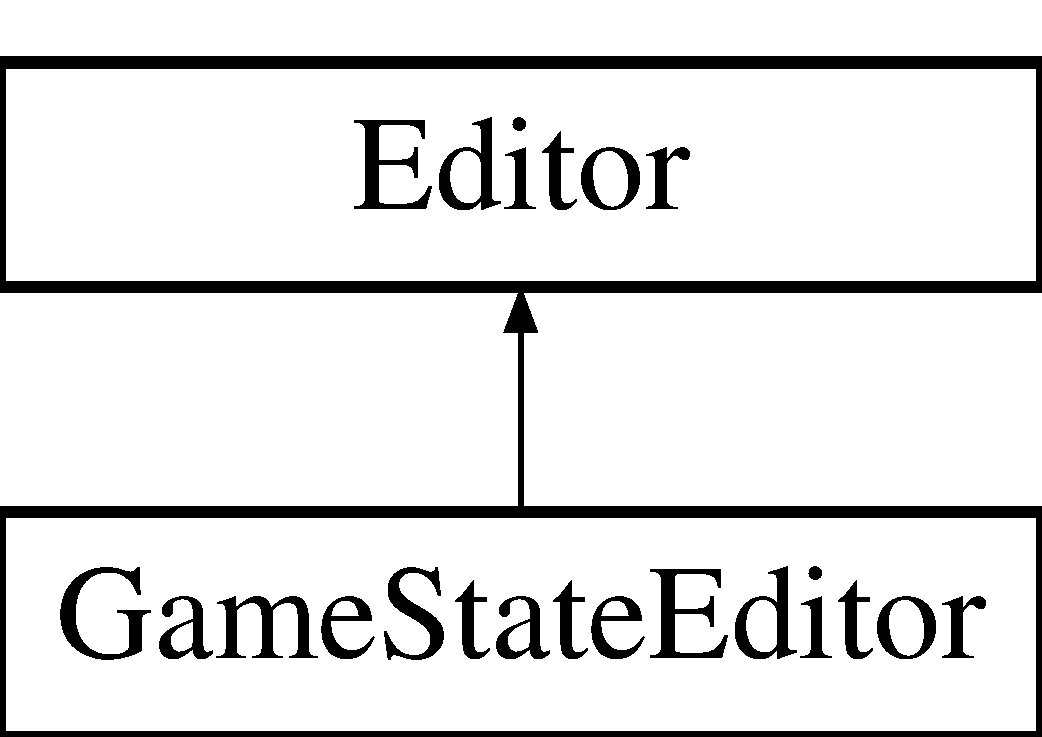
\includegraphics[height=2.000000cm]{class_game_state_editor}
\end{center}
\end{figure}
\subsection*{Public Member Functions}
\begin{DoxyCompactItemize}
\item 
\hypertarget{class_game_state_editor_a2fe1e0ec06ee8032b3b423c4f2451749}{override void {\bfseries On\-Inspector\-G\-U\-I} ()}\label{class_game_state_editor_a2fe1e0ec06ee8032b3b423c4f2451749}

\end{DoxyCompactItemize}
\subsection*{Static Public Member Functions}
\begin{DoxyCompactItemize}
\item 
static void \hyperlink{class_game_state_editor_a2ff679df4b2c28baef1a437bd0f656a6}{Create} ()
\begin{DoxyCompactList}\small\item\em Creates a Scriptable\-Object for \hyperlink{class_game_state}{Game\-State} from a Unity Menu context \end{DoxyCompactList}\end{DoxyCompactItemize}


\subsection{Member Function Documentation}
\hypertarget{class_game_state_editor_a2ff679df4b2c28baef1a437bd0f656a6}{\index{Game\-State\-Editor@{Game\-State\-Editor}!Create@{Create}}
\index{Create@{Create}!GameStateEditor@{Game\-State\-Editor}}
\subsubsection[{Create}]{\setlength{\rightskip}{0pt plus 5cm}static void Game\-State\-Editor.\-Create (
\begin{DoxyParamCaption}
{}
\end{DoxyParamCaption}
)\hspace{0.3cm}{\ttfamily [inline]}, {\ttfamily [static]}}}\label{class_game_state_editor_a2ff679df4b2c28baef1a437bd0f656a6}


Creates a Scriptable\-Object for \hyperlink{class_game_state}{Game\-State} from a Unity Menu context 



The documentation for this class was generated from the following file\-:\begin{DoxyCompactItemize}
\item 
/home/travis/build/temportalflux/\-Champ\-Net/\-Unity/\-Assets/\-Scripts/\-Editor/Game\-State\-Editor.\-cs\end{DoxyCompactItemize}

\hypertarget{interface_bit_serialize_attribute_1_1_i_serialization_module}{\section{Bit\-Serialize\-Attribute.\-I\-Serialization\-Module Interface Reference}
\label{interface_bit_serialize_attribute_1_1_i_serialization_module}\index{Bit\-Serialize\-Attribute.\-I\-Serialization\-Module@{Bit\-Serialize\-Attribute.\-I\-Serialization\-Module}}
}


The interface to use Serialization\-Module\{\-T\} in collections without knowing the type.  


Inheritance diagram for Bit\-Serialize\-Attribute.\-I\-Serialization\-Module\-:\begin{figure}[H]
\begin{center}
\leavevmode
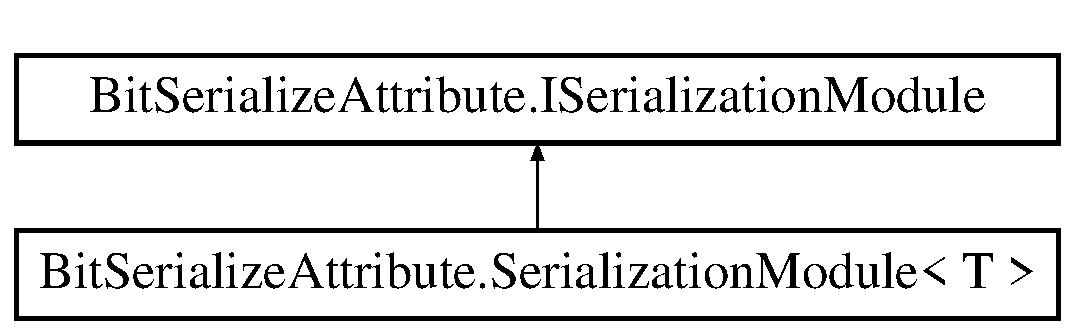
\includegraphics[height=2.000000cm]{interface_bit_serialize_attribute_1_1_i_serialization_module}
\end{center}
\end{figure}
\subsection*{Public Member Functions}
\begin{DoxyCompactItemize}
\item 
int \hyperlink{interface_bit_serialize_attribute_1_1_i_serialization_module_a057ba8b3168eb8a0999a329cca222cea}{Get\-Size} (object obj)
\begin{DoxyCompactList}\small\item\em Determine the size of some object -\/ effectively sizeof(object). \end{DoxyCompactList}\item 
byte\mbox{[}$\,$\mbox{]} \hyperlink{interface_bit_serialize_attribute_1_1_i_serialization_module_ad3b3d5f329538f550958a8342d9e0708}{Serialize} (object obj, byte\mbox{[}$\,$\mbox{]} data, int start)
\begin{DoxyCompactList}\small\item\em Serialize a specfic object into a byte array. Returns the byte\mbox{[}\mbox{]} with the populated data. \end{DoxyCompactList}\item 
object \hyperlink{interface_bit_serialize_attribute_1_1_i_serialization_module_a9c1c3c1a875354c8d3320e99c63da4a4}{Deserialize} (object obj, byte\mbox{[}$\,$\mbox{]} data, int start, Type type)
\begin{DoxyCompactList}\small\item\em Deserialize a byte array into an object. \end{DoxyCompactList}\end{DoxyCompactItemize}


\subsection{Detailed Description}
The interface to use Serialization\-Module\{\-T\} in collections without knowing the type. 



\subsection{Member Function Documentation}
\hypertarget{interface_bit_serialize_attribute_1_1_i_serialization_module_a9c1c3c1a875354c8d3320e99c63da4a4}{\index{Bit\-Serialize\-Attribute\-::\-I\-Serialization\-Module@{Bit\-Serialize\-Attribute\-::\-I\-Serialization\-Module}!Deserialize@{Deserialize}}
\index{Deserialize@{Deserialize}!BitSerializeAttribute::ISerializationModule@{Bit\-Serialize\-Attribute\-::\-I\-Serialization\-Module}}
\subsubsection[{Deserialize}]{\setlength{\rightskip}{0pt plus 5cm}object Bit\-Serialize\-Attribute.\-I\-Serialization\-Module.\-Deserialize (
\begin{DoxyParamCaption}
\item[{object}]{obj, }
\item[{byte\mbox{[}$\,$\mbox{]}}]{data, }
\item[{int}]{start, }
\item[{Type}]{type}
\end{DoxyParamCaption}
)}}\label{interface_bit_serialize_attribute_1_1_i_serialization_module_a9c1c3c1a875354c8d3320e99c63da4a4}


Deserialize a byte array into an object. 


\begin{DoxyParams}{Parameters}
{\em data} & the byte\mbox{[}\mbox{]} of data.\\
\hline
{\em start} & How far into the serialized data the object was put.\\
\hline
\end{DoxyParams}
\begin{DoxyReturn}{Returns}
object
\end{DoxyReturn}


Implemented in \hyperlink{class_bit_serialize_attribute_1_1_serialization_module_3_01_t_01_4_a7259a654093fa61bab6ef3766d13a12e}{Bit\-Serialize\-Attribute.\-Serialization\-Module$<$ T $>$}.

\hypertarget{interface_bit_serialize_attribute_1_1_i_serialization_module_a057ba8b3168eb8a0999a329cca222cea}{\index{Bit\-Serialize\-Attribute\-::\-I\-Serialization\-Module@{Bit\-Serialize\-Attribute\-::\-I\-Serialization\-Module}!Get\-Size@{Get\-Size}}
\index{Get\-Size@{Get\-Size}!BitSerializeAttribute::ISerializationModule@{Bit\-Serialize\-Attribute\-::\-I\-Serialization\-Module}}
\subsubsection[{Get\-Size}]{\setlength{\rightskip}{0pt plus 5cm}int Bit\-Serialize\-Attribute.\-I\-Serialization\-Module.\-Get\-Size (
\begin{DoxyParamCaption}
\item[{object}]{obj}
\end{DoxyParamCaption}
)}}\label{interface_bit_serialize_attribute_1_1_i_serialization_module_a057ba8b3168eb8a0999a329cca222cea}


Determine the size of some object -\/ effectively sizeof(object). 


\begin{DoxyParams}{Parameters}
{\em obj} & The object.\\
\hline
\end{DoxyParams}
\begin{DoxyReturn}{Returns}
int
\end{DoxyReturn}


Implemented in \hyperlink{class_bit_serialize_attribute_1_1_serialization_module_3_01_t_01_4_a2ab6b7e0f1e8eccfe929221a4c86c0b3}{Bit\-Serialize\-Attribute.\-Serialization\-Module$<$ T $>$}.

\hypertarget{interface_bit_serialize_attribute_1_1_i_serialization_module_ad3b3d5f329538f550958a8342d9e0708}{\index{Bit\-Serialize\-Attribute\-::\-I\-Serialization\-Module@{Bit\-Serialize\-Attribute\-::\-I\-Serialization\-Module}!Serialize@{Serialize}}
\index{Serialize@{Serialize}!BitSerializeAttribute::ISerializationModule@{Bit\-Serialize\-Attribute\-::\-I\-Serialization\-Module}}
\subsubsection[{Serialize}]{\setlength{\rightskip}{0pt plus 5cm}byte \mbox{[}$\,$\mbox{]} Bit\-Serialize\-Attribute.\-I\-Serialization\-Module.\-Serialize (
\begin{DoxyParamCaption}
\item[{object}]{obj, }
\item[{byte\mbox{[}$\,$\mbox{]}}]{data, }
\item[{int}]{start}
\end{DoxyParamCaption}
)}}\label{interface_bit_serialize_attribute_1_1_i_serialization_module_ad3b3d5f329538f550958a8342d9e0708}


Serialize a specfic object into a byte array. Returns the byte\mbox{[}\mbox{]} with the populated data. 


\begin{DoxyParams}{Parameters}
{\em obj} & The object to serialize.\\
\hline
{\em data} & The byte array of data.\\
\hline
{\em start} & How far into the data to put the object's serialized data.\\
\hline
\end{DoxyParams}
\begin{DoxyReturn}{Returns}
byte\mbox{[}\mbox{]}
\end{DoxyReturn}


Implemented in \hyperlink{class_bit_serialize_attribute_1_1_serialization_module_3_01_t_01_4_a566f48c068bafbe25a9d3371afb83892}{Bit\-Serialize\-Attribute.\-Serialization\-Module$<$ T $>$}.



The documentation for this interface was generated from the following file\-:\begin{DoxyCompactItemize}
\item 
/home/travis/build/temportalflux/\-Champ\-Net/\-Unity/\-Assets/\-Scripts/\-Attribute/Bit\-Serialize\-Attribute.\-cs\end{DoxyCompactItemize}

\hypertarget{interface_i_serializing}{\section{I\-Serializing Interface Reference}
\label{interface_i_serializing}\index{I\-Serializing@{I\-Serializing}}
}
Inheritance diagram for I\-Serializing\-:\begin{figure}[H]
\begin{center}
\leavevmode
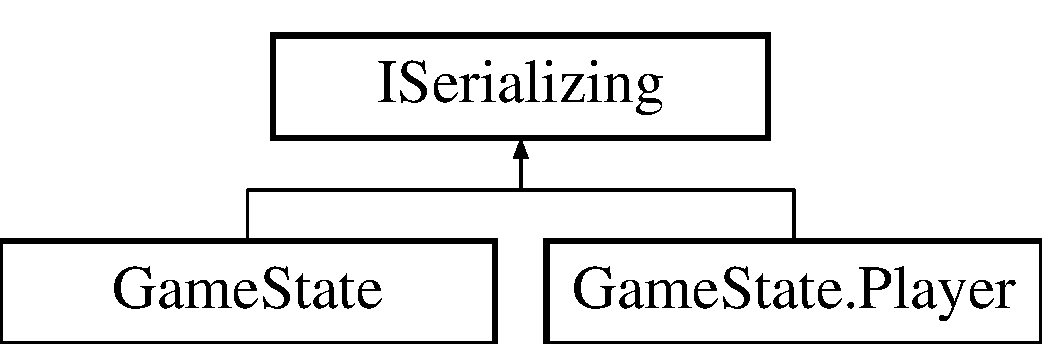
\includegraphics[height=2.000000cm]{interface_i_serializing}
\end{center}
\end{figure}
\subsection*{Public Member Functions}
\begin{DoxyCompactItemize}
\item 
int \hyperlink{interface_i_serializing_a9e6ea0afaeac8d1d57e20579f87bebe2}{Get\-Size} ()
\begin{DoxyCompactList}\small\item\em Returns the size of the packet (the size for a potential byte\mbox{[}\mbox{]}) \end{DoxyCompactList}\item 
void \hyperlink{interface_i_serializing_ac31a44c2358a197e774fa3f79cc80356}{Serialize} (ref byte\mbox{[}$\,$\mbox{]} data, ref int last\-Index)
\begin{DoxyCompactList}\small\item\em Serializes data from this event into a byte array \end{DoxyCompactList}\item 
void \hyperlink{interface_i_serializing_a92f8ba3a06d21e7b01e37411e4e3145c}{Deserialize} (byte\mbox{[}$\,$\mbox{]} data, ref int last\-Index)
\begin{DoxyCompactList}\small\item\em Deserializes data from a byte array into this event's data \end{DoxyCompactList}\end{DoxyCompactItemize}


\subsection{Member Function Documentation}
\hypertarget{interface_i_serializing_a92f8ba3a06d21e7b01e37411e4e3145c}{\index{I\-Serializing@{I\-Serializing}!Deserialize@{Deserialize}}
\index{Deserialize@{Deserialize}!ISerializing@{I\-Serializing}}
\subsubsection[{Deserialize}]{\setlength{\rightskip}{0pt plus 5cm}void I\-Serializing.\-Deserialize (
\begin{DoxyParamCaption}
\item[{byte\mbox{[}$\,$\mbox{]}}]{data, }
\item[{ref int}]{last\-Index}
\end{DoxyParamCaption}
)}}\label{interface_i_serializing_a92f8ba3a06d21e7b01e37411e4e3145c}


Deserializes data from a byte array into this event's data 


\begin{DoxyParams}{Parameters}
{\em data} & The data.\\
\hline
{\em last\-Index} & The last index.\\
\hline
\end{DoxyParams}


Author\-: Dustin Yost 

Implemented in \hyperlink{class_game_state_aa5f956de2c49182fbe5fc32e9d2ca431}{Game\-State}, and \hyperlink{struct_game_state_1_1_player_aaf7c5b93f45be35c3501626cb6759c0b}{Game\-State.\-Player}.

\hypertarget{interface_i_serializing_a9e6ea0afaeac8d1d57e20579f87bebe2}{\index{I\-Serializing@{I\-Serializing}!Get\-Size@{Get\-Size}}
\index{Get\-Size@{Get\-Size}!ISerializing@{I\-Serializing}}
\subsubsection[{Get\-Size}]{\setlength{\rightskip}{0pt plus 5cm}int I\-Serializing.\-Get\-Size (
\begin{DoxyParamCaption}
{}
\end{DoxyParamCaption}
)}}\label{interface_i_serializing_a9e6ea0afaeac8d1d57e20579f87bebe2}


Returns the size of the packet (the size for a potential byte\mbox{[}\mbox{]}) 

\begin{DoxyReturn}{Returns}
the integer length of a byte array to hold this event's data 
\end{DoxyReturn}


Author\-: Dustin Yost 

Implemented in \hyperlink{class_game_state_a57d152b243c11aa86e7ba0f07b4bd0dd}{Game\-State}, and \hyperlink{struct_game_state_1_1_player_a58e1b4e7eaca487703abf36826e41c45}{Game\-State.\-Player}.

\hypertarget{interface_i_serializing_ac31a44c2358a197e774fa3f79cc80356}{\index{I\-Serializing@{I\-Serializing}!Serialize@{Serialize}}
\index{Serialize@{Serialize}!ISerializing@{I\-Serializing}}
\subsubsection[{Serialize}]{\setlength{\rightskip}{0pt plus 5cm}void I\-Serializing.\-Serialize (
\begin{DoxyParamCaption}
\item[{ref byte\mbox{[}$\,$\mbox{]}}]{data, }
\item[{ref int}]{last\-Index}
\end{DoxyParamCaption}
)}}\label{interface_i_serializing_ac31a44c2358a197e774fa3f79cc80356}


Serializes data from this event into a byte array 


\begin{DoxyParams}{Parameters}
{\em data} & The data.\\
\hline
{\em last\-Index} & The last index.\\
\hline
\end{DoxyParams}


Author\-: Dustin Yost 

Implemented in \hyperlink{class_game_state_af57a06c77a763e8b57841bab79c9b12f}{Game\-State}, and \hyperlink{struct_game_state_1_1_player_aa8df830f0a0bcfbfb263a634d125c3a5}{Game\-State.\-Player}.



The documentation for this interface was generated from the following file\-:\begin{DoxyCompactItemize}
\item 
/home/travis/build/temportalflux/\-Champ\-Net/\-Unity/\-Assets/\-Scripts/\-Network/events/I\-Serializing.\-cs\end{DoxyCompactItemize}

\hypertarget{class_keeper_system}{\section{Keeper\-System Class Reference}
\label{class_keeper_system}\index{Keeper\-System@{Keeper\-System}}
}
Inheritance diagram for Keeper\-System\-:\begin{figure}[H]
\begin{center}
\leavevmode
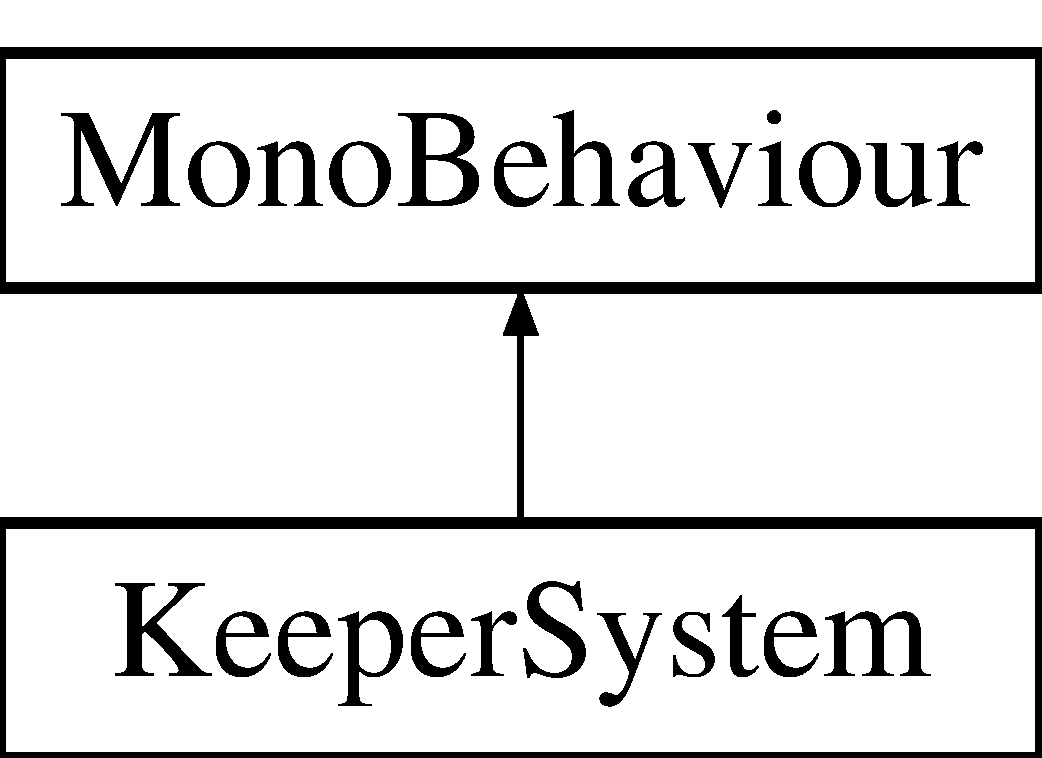
\includegraphics[height=2.000000cm]{class_keeper_system}
\end{center}
\end{figure}
\subsection*{Public Attributes}
\begin{DoxyCompactItemize}
\item 
\hypertarget{class_keeper_system_a351a9a8819200deb7e235c6ef2e059a6}{string {\bfseries keepername}}\label{class_keeper_system_a351a9a8819200deb7e235c6ef2e059a6}

\item 
\hypertarget{class_keeper_system_a10dc4e4959293cc3a39eda19d35e5c8c}{List$<$ \hyperlink{class_monster_data_object}{Monster\-Data\-Object} $>$ {\bfseries monsters}}\label{class_keeper_system_a10dc4e4959293cc3a39eda19d35e5c8c}

\item 
\hypertarget{class_keeper_system_a032c60966af729c76e4a09e1fa6dbadb}{int {\bfseries wins}}\label{class_keeper_system_a032c60966af729c76e4a09e1fa6dbadb}

\item 
\hypertarget{class_keeper_system_ab64ebb44295e23d56fc640ff92dfe5d2}{int {\bfseries losses}}\label{class_keeper_system_ab64ebb44295e23d56fc640ff92dfe5d2}

\end{DoxyCompactItemize}


The documentation for this class was generated from the following file\-:\begin{DoxyCompactItemize}
\item 
/home/travis/build/temportalflux/\-Champ\-Net/\-Unity/\-Assets/\-Scripts/\-Player/Keeper\-System.\-cs\end{DoxyCompactItemize}

\hypertarget{class_manager_transitions}{\section{Manager\-Transitions Class Reference}
\label{class_manager_transitions}\index{Manager\-Transitions@{Manager\-Transitions}}
}
Inheritance diagram for Manager\-Transitions\-:\begin{figure}[H]
\begin{center}
\leavevmode
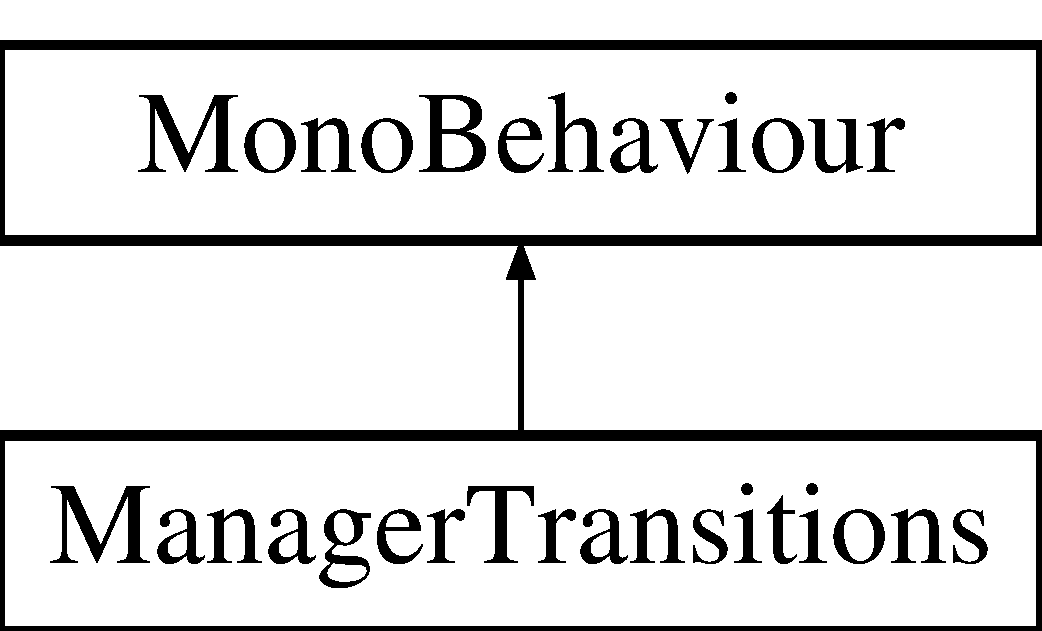
\includegraphics[height=2.000000cm]{class_manager_transitions}
\end{center}
\end{figure}
\subsection*{Public Member Functions}
\begin{DoxyCompactItemize}
\item 
\hypertarget{class_manager_transitions_af143a676b64ad9405dee52e0b3524db0}{delegate void {\bfseries On\-Transition\-Finish} ()}\label{class_manager_transitions_af143a676b64ad9405dee52e0b3524db0}

\item 
bool \hyperlink{class_manager_transitions_aeb23059e823543ba248f10d138ebf045}{trigger\-Load\-Async} (string next\-Scene, \hyperlink{class_transition}{Transition} transition, Load\-Scene\-Mode load\-Mode, On\-Transition\-Finish on\-Finish=null)
\item 
\hypertarget{class_manager_transitions_a5d65799742ec1d9c71abf4b69688bc80}{bool {\bfseries trigger\-Un\-Load\-Async} (string next\-Scene, \hyperlink{class_transition}{Transition} transition, Load\-Scene\-Mode load\-Mode, On\-Transition\-Finish on\-Finish=null)}\label{class_manager_transitions_a5d65799742ec1d9c71abf4b69688bc80}

\item 
\hypertarget{class_manager_transitions_a7809ff8c65986d89284ae9a7ad570355}{void {\bfseries trigger\-Exit} ()}\label{class_manager_transitions_a7809ff8c65986d89284ae9a7ad570355}

\end{DoxyCompactItemize}
\subsection*{Properties}
\begin{DoxyCompactItemize}
\item 
\hypertarget{class_manager_transitions_ad87cd9fb9a0e05bb97be220bf3f782e1}{static \hyperlink{class_manager_transitions}{Manager\-Transitions} {\bfseries I\-N\-S\-T\-A\-N\-C\-E}\hspace{0.3cm}{\ttfamily  \mbox{[}get\mbox{]}}}\label{class_manager_transitions_ad87cd9fb9a0e05bb97be220bf3f782e1}

\end{DoxyCompactItemize}


\subsection{Detailed Description}
Author\-: Dustin Yost Static component class which handles transitioning between scenes 

\subsection{Member Function Documentation}
\hypertarget{class_manager_transitions_aeb23059e823543ba248f10d138ebf045}{\index{Manager\-Transitions@{Manager\-Transitions}!trigger\-Load\-Async@{trigger\-Load\-Async}}
\index{trigger\-Load\-Async@{trigger\-Load\-Async}!ManagerTransitions@{Manager\-Transitions}}
\subsubsection[{trigger\-Load\-Async}]{\setlength{\rightskip}{0pt plus 5cm}bool Manager\-Transitions.\-trigger\-Load\-Async (
\begin{DoxyParamCaption}
\item[{string}]{next\-Scene, }
\item[{{\bf Transition}}]{transition, }
\item[{Load\-Scene\-Mode}]{load\-Mode, }
\item[{On\-Transition\-Finish}]{on\-Finish = {\ttfamily null}}
\end{DoxyParamCaption}
)\hspace{0.3cm}{\ttfamily [inline]}}}\label{class_manager_transitions_aeb23059e823543ba248f10d138ebf045}
Trigger a loading of some scene asynchronously with some transition 

The documentation for this class was generated from the following file\-:\begin{DoxyCompactItemize}
\item 
/home/travis/build/temportalflux/\-Champ\-Net/\-Unity/\-Assets/\-Scripts/\-Transitions/Manager\-Transitions.\-cs\end{DoxyCompactItemize}

\hypertarget{class_minimap_handler}{\section{Minimap\-Handler Class Reference}
\label{class_minimap_handler}\index{Minimap\-Handler@{Minimap\-Handler}}
}
Inheritance diagram for Minimap\-Handler\-:\begin{figure}[H]
\begin{center}
\leavevmode
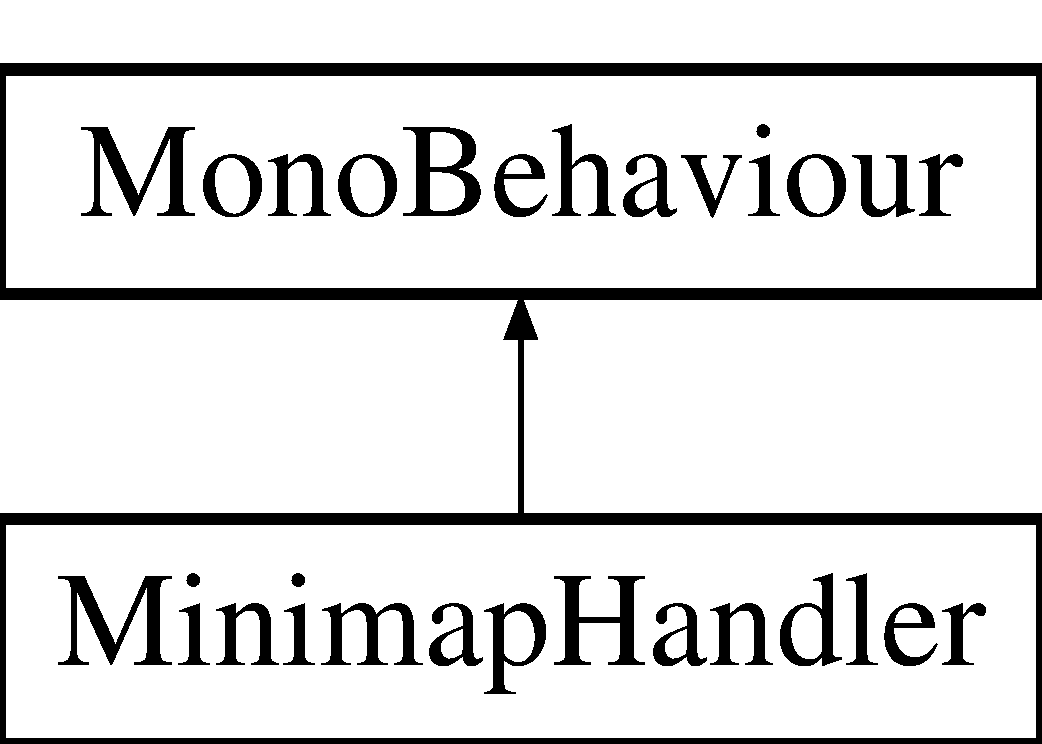
\includegraphics[height=2.000000cm]{class_minimap_handler}
\end{center}
\end{figure}
\subsection*{Public Attributes}
\begin{DoxyCompactItemize}
\item 
\hypertarget{class_minimap_handler_a29ccc8d8bee56eaf345fbcdddb369166}{Camera {\bfseries Minimap\-Camera}}\label{class_minimap_handler_a29ccc8d8bee56eaf345fbcdddb369166}

\end{DoxyCompactItemize}


The documentation for this class was generated from the following file\-:\begin{DoxyCompactItemize}
\item 
/home/travis/build/temportalflux/\-Champ\-Net/\-Unity/\-Assets/\-Scripts/\-U\-I/\-Mini\-Map/Minimap\-Handler.\-cs\end{DoxyCompactItemize}

\hypertarget{class_monster_data_object}{\section{Monster\-Data\-Object Class Reference}
\label{class_monster_data_object}\index{Monster\-Data\-Object@{Monster\-Data\-Object}}
}
\subsection*{Public Member Functions}
\begin{DoxyCompactItemize}
\item 
int \hyperlink{class_monster_data_object_a6dd85baaa39abaac720a36b71db7536e}{Get\-Monster\-Attack\-Stat} (Move\-Kind physical\-Or\-Special, bool apply\-Stat\-Stages=false)
\begin{DoxyCompactList}\small\item\em Get the attack stat based on the move kind \end{DoxyCompactList}\item 
int \hyperlink{class_monster_data_object_a1eda550eeb621625d872b66b1c27eba7}{Get\-Monster\-Defense\-Stat} (Move\-Kind physical\-Or\-Special, bool apply\-Stat\-Stages=false)
\begin{DoxyCompactList}\small\item\em Get the defense stat based on the move kind. \end{DoxyCompactList}\end{DoxyCompactItemize}
\subsection*{Public Attributes}
\begin{DoxyCompactItemize}
\item 
\hypertarget{class_monster_data_object_a32f219c168636419992aa379f59c9ff0}{\hyperlink{class_monster_stat}{Monster\-Stat} {\bfseries monster\-Stat}}\label{class_monster_data_object_a32f219c168636419992aa379f59c9ff0}

\item 
\hypertarget{class_monster_data_object_ac1197136faf77c440906bade6ee2b690}{int {\bfseries stat\-Stage\-Attack}}\label{class_monster_data_object_ac1197136faf77c440906bade6ee2b690}

\item 
\hypertarget{class_monster_data_object_a0a292ad39496e69386b877f3ddaeb123}{int {\bfseries stat\-Stage\-Defense}}\label{class_monster_data_object_a0a292ad39496e69386b877f3ddaeb123}

\item 
\hypertarget{class_monster_data_object_a70677e28a5a8ba6ae3a2cad0ffdb0c47}{int {\bfseries stat\-Stage\-Special\-Attack}}\label{class_monster_data_object_a70677e28a5a8ba6ae3a2cad0ffdb0c47}

\item 
\hypertarget{class_monster_data_object_a1aca4196d55b289763cced6b55b2ddc8}{int {\bfseries stat\-Stage\-Special\-Defense}}\label{class_monster_data_object_a1aca4196d55b289763cced6b55b2ddc8}

\item 
\hypertarget{class_monster_data_object_a6572a7633fc1cd965e2c6c0ab7b86f9f}{int {\bfseries stat\-Stage\-Speed}}\label{class_monster_data_object_a6572a7633fc1cd965e2c6c0ab7b86f9f}

\end{DoxyCompactItemize}
\subsection*{Properties}
\begin{DoxyCompactItemize}
\item 
\hypertarget{class_monster_data_object_a6c67d5bab62fb649e01355b52ccf16ba}{string {\bfseries Get\-Monster\-Name}\hspace{0.3cm}{\ttfamily  \mbox{[}get\mbox{]}}}\label{class_monster_data_object_a6c67d5bab62fb649e01355b52ccf16ba}

\item 
\hypertarget{class_monster_data_object_a0d1ed24b79b82bb78c26811aa34b3ac7}{List$<$ Monster\-Type $>$ {\bfseries Get\-Types}\hspace{0.3cm}{\ttfamily  \mbox{[}get\mbox{]}}}\label{class_monster_data_object_a0d1ed24b79b82bb78c26811aa34b3ac7}

\item 
\hypertarget{class_monster_data_object_ae1c3d104809049c612c9a1b6a61664be}{int {\bfseries Get\-Attack}\hspace{0.3cm}{\ttfamily  \mbox{[}get\mbox{]}}}\label{class_monster_data_object_ae1c3d104809049c612c9a1b6a61664be}

\item 
\hypertarget{class_monster_data_object_a2409f379ef651b10b5d7638154da7421}{int {\bfseries Get\-Defense}\hspace{0.3cm}{\ttfamily  \mbox{[}get\mbox{]}}}\label{class_monster_data_object_a2409f379ef651b10b5d7638154da7421}

\item 
\hypertarget{class_monster_data_object_a5beec2bbced5d78744aa0ea784218357}{int {\bfseries Get\-Special\-Attack}\hspace{0.3cm}{\ttfamily  \mbox{[}get\mbox{]}}}\label{class_monster_data_object_a5beec2bbced5d78744aa0ea784218357}

\item 
\hypertarget{class_monster_data_object_aafcc2ea03b96291140ebcb40331e4cd2}{int {\bfseries Get\-Special\-Defense}\hspace{0.3cm}{\ttfamily  \mbox{[}get\mbox{]}}}\label{class_monster_data_object_aafcc2ea03b96291140ebcb40331e4cd2}

\item 
\hypertarget{class_monster_data_object_a0d7639dc92ae01942b1b996565eff2ae}{int {\bfseries Get\-Speed}\hspace{0.3cm}{\ttfamily  \mbox{[}get\mbox{]}}}\label{class_monster_data_object_a0d7639dc92ae01942b1b996565eff2ae}

\item 
\hypertarget{class_monster_data_object_aced78f5f04d3dbb79a0f8291fbe118bd}{List$<$ \hyperlink{class_attack_object}{Attack\-Object} $>$ {\bfseries Get\-Available\-Attacks}\hspace{0.3cm}{\ttfamily  \mbox{[}get\mbox{]}}}\label{class_monster_data_object_aced78f5f04d3dbb79a0f8291fbe118bd}

\end{DoxyCompactItemize}


\subsection{Member Function Documentation}
\hypertarget{class_monster_data_object_a6dd85baaa39abaac720a36b71db7536e}{\index{Monster\-Data\-Object@{Monster\-Data\-Object}!Get\-Monster\-Attack\-Stat@{Get\-Monster\-Attack\-Stat}}
\index{Get\-Monster\-Attack\-Stat@{Get\-Monster\-Attack\-Stat}!MonsterDataObject@{Monster\-Data\-Object}}
\subsubsection[{Get\-Monster\-Attack\-Stat}]{\setlength{\rightskip}{0pt plus 5cm}int Monster\-Data\-Object.\-Get\-Monster\-Attack\-Stat (
\begin{DoxyParamCaption}
\item[{Move\-Kind}]{physical\-Or\-Special, }
\item[{bool}]{apply\-Stat\-Stages = {\ttfamily false}}
\end{DoxyParamCaption}
)\hspace{0.3cm}{\ttfamily [inline]}}}\label{class_monster_data_object_a6dd85baaa39abaac720a36b71db7536e}


Get the attack stat based on the move kind 


\begin{DoxyParams}{Parameters}
{\em physical\-Or\-Special} & is the move physical or special?\\
\hline
{\em apply\-Stat\-Stages} & if {\ttfamily true} then the stat stages are applied\\
\hline
\end{DoxyParams}
\begin{DoxyReturn}{Returns}
the modified attack stat
\end{DoxyReturn}
\hypertarget{class_monster_data_object_a1eda550eeb621625d872b66b1c27eba7}{\index{Monster\-Data\-Object@{Monster\-Data\-Object}!Get\-Monster\-Defense\-Stat@{Get\-Monster\-Defense\-Stat}}
\index{Get\-Monster\-Defense\-Stat@{Get\-Monster\-Defense\-Stat}!MonsterDataObject@{Monster\-Data\-Object}}
\subsubsection[{Get\-Monster\-Defense\-Stat}]{\setlength{\rightskip}{0pt plus 5cm}int Monster\-Data\-Object.\-Get\-Monster\-Defense\-Stat (
\begin{DoxyParamCaption}
\item[{Move\-Kind}]{physical\-Or\-Special, }
\item[{bool}]{apply\-Stat\-Stages = {\ttfamily false}}
\end{DoxyParamCaption}
)\hspace{0.3cm}{\ttfamily [inline]}}}\label{class_monster_data_object_a1eda550eeb621625d872b66b1c27eba7}


Get the defense stat based on the move kind. 


\begin{DoxyParams}{Parameters}
{\em physical\-Or\-Special} & is the move physical or special?\\
\hline
{\em apply\-Stat\-Stages} & if {\ttfamily true} then the stat stages are applied\\
\hline
\end{DoxyParams}
\begin{DoxyReturn}{Returns}
the modified defense stat
\end{DoxyReturn}


The documentation for this class was generated from the following file\-:\begin{DoxyCompactItemize}
\item 
/home/travis/build/temportalflux/\-Champ\-Net/\-Unity/\-Assets/\-Scripts/Monster\-Data\-Object.\-cs\end{DoxyCompactItemize}

\hypertarget{class_monster_data_object_editor}{\section{Monster\-Data\-Object\-Editor Class Reference}
\label{class_monster_data_object_editor}\index{Monster\-Data\-Object\-Editor@{Monster\-Data\-Object\-Editor}}
}
Inheritance diagram for Monster\-Data\-Object\-Editor\-:\begin{figure}[H]
\begin{center}
\leavevmode
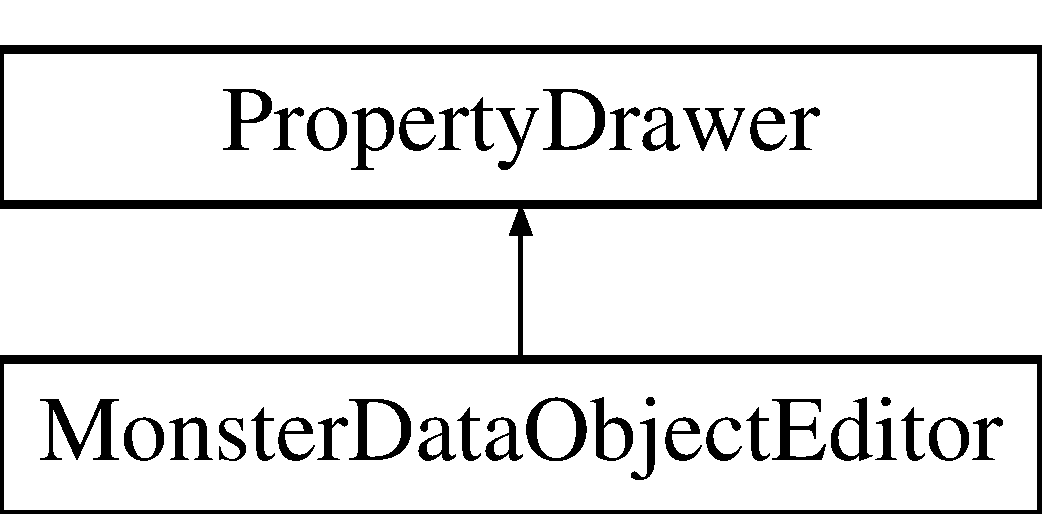
\includegraphics[height=2.000000cm]{class_monster_data_object_editor}
\end{center}
\end{figure}
\subsection*{Public Member Functions}
\begin{DoxyCompactItemize}
\item 
\hypertarget{class_monster_data_object_editor_a6f68c967f408d0c49b48518848c4a6ed}{override void {\bfseries On\-G\-U\-I} (Rect position, Serialized\-Property property, G\-U\-I\-Content label)}\label{class_monster_data_object_editor_a6f68c967f408d0c49b48518848c4a6ed}

\end{DoxyCompactItemize}


The documentation for this class was generated from the following file\-:\begin{DoxyCompactItemize}
\item 
/home/travis/build/temportalflux/\-Champ\-Net/\-Unity/\-Assets/\-Scripts/\-Editor/Monster\-Data\-Object\-Editor.\-cs\end{DoxyCompactItemize}

\hypertarget{class_monster_stat}{\section{Monster\-Stat Class Reference}
\label{class_monster_stat}\index{Monster\-Stat@{Monster\-Stat}}
}
Inheritance diagram for Monster\-Stat\-:\begin{figure}[H]
\begin{center}
\leavevmode
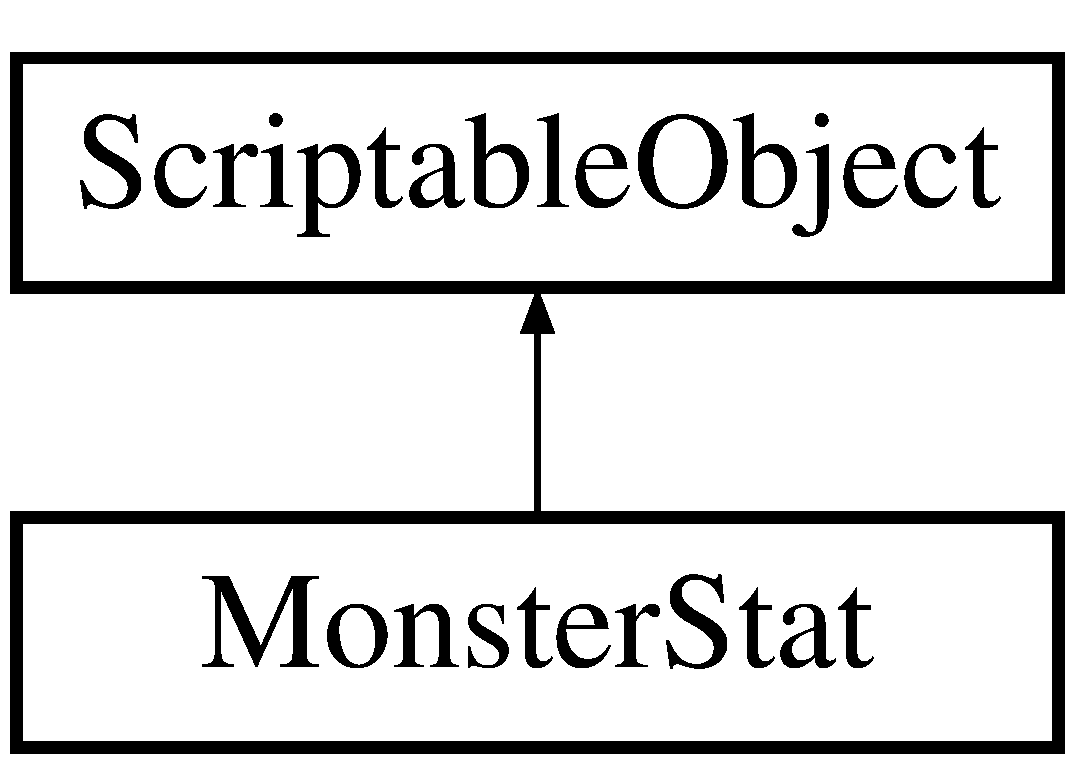
\includegraphics[height=2.000000cm]{class_monster_stat}
\end{center}
\end{figure}
\subsection*{Public Attributes}
\begin{DoxyCompactItemize}
\item 
\hypertarget{class_monster_stat_ae1f09abad9691a1b0df3b3a3575a64e3}{string {\bfseries monster\-Name}}\label{class_monster_stat_ae1f09abad9691a1b0df3b3a3575a64e3}

\item 
\hypertarget{class_monster_stat_a1699a9350fa5b1b0cece5a0a5fdd112a}{Sprite {\bfseries monster\-Picture}}\label{class_monster_stat_a1699a9350fa5b1b0cece5a0a5fdd112a}

\item 
\hypertarget{class_monster_stat_a01771faf888660584ddf5e134d4da3fb}{List$<$ Monster\-Type $>$ {\bfseries types}}\label{class_monster_stat_a01771faf888660584ddf5e134d4da3fb}

\item 
\hypertarget{class_monster_stat_a3f84d73d947c10926862b904308f01ee}{int {\bfseries max\-Hp}}\label{class_monster_stat_a3f84d73d947c10926862b904308f01ee}

\item 
\hypertarget{class_monster_stat_aa712f00d29d985ecbf192710dd093e42}{int {\bfseries attack}}\label{class_monster_stat_aa712f00d29d985ecbf192710dd093e42}

\item 
\hypertarget{class_monster_stat_adcd2f958be981766592eefec3d7cd7da}{int {\bfseries defense}}\label{class_monster_stat_adcd2f958be981766592eefec3d7cd7da}

\item 
\hypertarget{class_monster_stat_ad1ef4ed9e67df473269df08ba716ce0e}{int {\bfseries special\-Attack}}\label{class_monster_stat_ad1ef4ed9e67df473269df08ba716ce0e}

\item 
\hypertarget{class_monster_stat_a38187f97efd1e52b77340058ecef8198}{int {\bfseries special\-Defense}}\label{class_monster_stat_a38187f97efd1e52b77340058ecef8198}

\item 
\hypertarget{class_monster_stat_a8e1945c1a296695622bada26319ff9e3}{int {\bfseries speed}}\label{class_monster_stat_a8e1945c1a296695622bada26319ff9e3}

\item 
\hypertarget{class_monster_stat_ae5ba7dc95fd5115dfed29cfeaafae51f}{List$<$ \hyperlink{class_attack_object}{Attack\-Object} $>$ {\bfseries available\-Attacks}}\label{class_monster_stat_ae5ba7dc95fd5115dfed29cfeaafae51f}

\end{DoxyCompactItemize}


The documentation for this class was generated from the following file\-:\begin{DoxyCompactItemize}
\item 
/home/travis/build/temportalflux/\-Champ\-Net/\-Unity/\-Assets/\-Scripts/\-Monster\-Scriptable\-Objects/Monster\-Stat.\-cs\end{DoxyCompactItemize}

\hypertarget{class_net_interface}{\section{Net\-Interface Class Reference}
\label{class_net_interface}\index{Net\-Interface@{Net\-Interface}}
}


The interface to work with the plugin to fetch and send packet data  


Inheritance diagram for Net\-Interface\-:\begin{figure}[H]
\begin{center}
\leavevmode
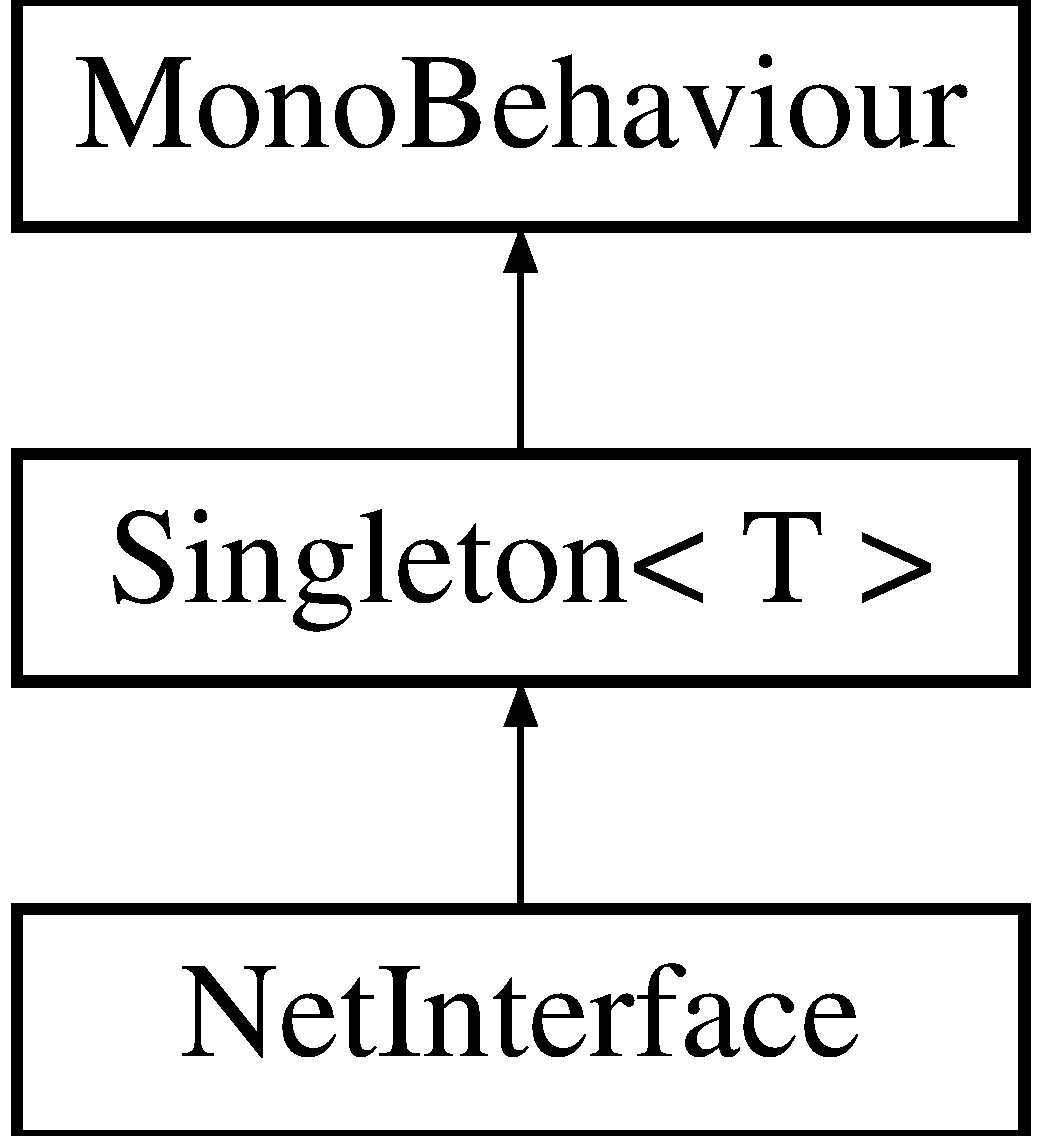
\includegraphics[height=3.000000cm]{class_net_interface}
\end{center}
\end{figure}
\subsection*{Public Member Functions}
\begin{DoxyCompactItemize}
\item 
void \hyperlink{class_net_interface_a565fb35ea7ed5e364902aa8bd0bc6bf9}{Connect} (string address, int port)
\begin{DoxyCompactList}\small\item\em Starts the client, connects the specified address and port. \end{DoxyCompactList}\item 
void \hyperlink{class_net_interface_ae0be68e392f32d422325ac54fcaa7cae}{Disconnect} ()
\begin{DoxyCompactList}\small\item\em Disconnects from the server. \end{DoxyCompactList}\item 
void \hyperlink{class_net_interface_a3ed4f694a9f2083af9ea38ed2a554404}{Dispatch} (Event\-Network evt)
\begin{DoxyCompactList}\small\item\em Dispatches the specified event. \end{DoxyCompactList}\item 
void \hyperlink{class_net_interface_a0cf4580da2218baff890af79fd606722}{Dispatch} (Event\-Network evt, string address, int port)
\begin{DoxyCompactList}\small\item\em Dispatches the specified event. \end{DoxyCompactList}\item 
Key\-Value\-Pair$<$ string, int $>$ \hyperlink{class_net_interface_a18dfbf82b7c690b9abf4ae9ed9aaddcd}{get\-Server} ()
\begin{DoxyCompactList}\small\item\em Gets the server I\-P details. \end{DoxyCompactList}\end{DoxyCompactItemize}
\subsection*{Properties}
\begin{DoxyCompactItemize}
\item 
static \hyperlink{class_net_interface}{Net\-Interface} \hyperlink{class_net_interface_a58a14d53d9e16a56849ecf2d13141d30}{I\-N\-S\-T\-A\-N\-C\-E}\hspace{0.3cm}{\ttfamily  \mbox{[}get\mbox{]}}
\begin{DoxyCompactList}\small\item\em Gets the instance. \end{DoxyCompactList}\end{DoxyCompactItemize}
\subsection*{Additional Inherited Members}


\subsection{Detailed Description}
The interface to work with the plugin to fetch and send packet data 

Author\-: Dustin Yost 

\subsection{Member Function Documentation}
\hypertarget{class_net_interface_a565fb35ea7ed5e364902aa8bd0bc6bf9}{\index{Net\-Interface@{Net\-Interface}!Connect@{Connect}}
\index{Connect@{Connect}!NetInterface@{Net\-Interface}}
\subsubsection[{Connect}]{\setlength{\rightskip}{0pt plus 5cm}void Net\-Interface.\-Connect (
\begin{DoxyParamCaption}
\item[{string}]{address, }
\item[{int}]{port}
\end{DoxyParamCaption}
)\hspace{0.3cm}{\ttfamily [inline]}}}\label{class_net_interface_a565fb35ea7ed5e364902aa8bd0bc6bf9}


Starts the client, connects the specified address and port. 


\begin{DoxyParams}{Parameters}
{\em address} & The address.\\
\hline
{\em port} & The port.\\
\hline
\end{DoxyParams}


Author\-: Dustin Yost \hypertarget{class_net_interface_ae0be68e392f32d422325ac54fcaa7cae}{\index{Net\-Interface@{Net\-Interface}!Disconnect@{Disconnect}}
\index{Disconnect@{Disconnect}!NetInterface@{Net\-Interface}}
\subsubsection[{Disconnect}]{\setlength{\rightskip}{0pt plus 5cm}void Net\-Interface.\-Disconnect (
\begin{DoxyParamCaption}
{}
\end{DoxyParamCaption}
)\hspace{0.3cm}{\ttfamily [inline]}}}\label{class_net_interface_ae0be68e392f32d422325ac54fcaa7cae}


Disconnects from the server. 

Author\-: Dustin Yost \hypertarget{class_net_interface_a3ed4f694a9f2083af9ea38ed2a554404}{\index{Net\-Interface@{Net\-Interface}!Dispatch@{Dispatch}}
\index{Dispatch@{Dispatch}!NetInterface@{Net\-Interface}}
\subsubsection[{Dispatch}]{\setlength{\rightskip}{0pt plus 5cm}void Net\-Interface.\-Dispatch (
\begin{DoxyParamCaption}
\item[{Event\-Network}]{evt}
\end{DoxyParamCaption}
)\hspace{0.3cm}{\ttfamily [inline]}}}\label{class_net_interface_a3ed4f694a9f2083af9ea38ed2a554404}


Dispatches the specified event. 


\begin{DoxyParams}{Parameters}
{\em evt} & The evt.\\
\hline
\end{DoxyParams}
\hypertarget{class_net_interface_a0cf4580da2218baff890af79fd606722}{\index{Net\-Interface@{Net\-Interface}!Dispatch@{Dispatch}}
\index{Dispatch@{Dispatch}!NetInterface@{Net\-Interface}}
\subsubsection[{Dispatch}]{\setlength{\rightskip}{0pt plus 5cm}void Net\-Interface.\-Dispatch (
\begin{DoxyParamCaption}
\item[{Event\-Network}]{evt, }
\item[{string}]{address, }
\item[{int}]{port}
\end{DoxyParamCaption}
)\hspace{0.3cm}{\ttfamily [inline]}}}\label{class_net_interface_a0cf4580da2218baff890af79fd606722}


Dispatches the specified event. 


\begin{DoxyParams}{Parameters}
{\em evt} & The event.\\
\hline
{\em address} & The server address.\\
\hline
{\em port} & The server port.\\
\hline
\end{DoxyParams}


Author\-: Jake Ruth \hypertarget{class_net_interface_a18dfbf82b7c690b9abf4ae9ed9aaddcd}{\index{Net\-Interface@{Net\-Interface}!get\-Server@{get\-Server}}
\index{get\-Server@{get\-Server}!NetInterface@{Net\-Interface}}
\subsubsection[{get\-Server}]{\setlength{\rightskip}{0pt plus 5cm}Key\-Value\-Pair$<$string, int$>$ Net\-Interface.\-get\-Server (
\begin{DoxyParamCaption}
{}
\end{DoxyParamCaption}
)\hspace{0.3cm}{\ttfamily [inline]}}}\label{class_net_interface_a18dfbf82b7c690b9abf4ae9ed9aaddcd}


Gets the server I\-P details. 

\begin{DoxyReturn}{Returns}
the server address/port
\end{DoxyReturn}


Author\-: Dustin Yost 

\subsection{Property Documentation}
\hypertarget{class_net_interface_a58a14d53d9e16a56849ecf2d13141d30}{\index{Net\-Interface@{Net\-Interface}!I\-N\-S\-T\-A\-N\-C\-E@{I\-N\-S\-T\-A\-N\-C\-E}}
\index{I\-N\-S\-T\-A\-N\-C\-E@{I\-N\-S\-T\-A\-N\-C\-E}!NetInterface@{Net\-Interface}}
\subsubsection[{I\-N\-S\-T\-A\-N\-C\-E}]{\setlength{\rightskip}{0pt plus 5cm}{\bf Net\-Interface} Net\-Interface.\-I\-N\-S\-T\-A\-N\-C\-E\hspace{0.3cm}{\ttfamily [static]}, {\ttfamily [get]}}}\label{class_net_interface_a58a14d53d9e16a56849ecf2d13141d30}


Gets the instance. 

The instance. 

The documentation for this class was generated from the following file\-:\begin{DoxyCompactItemize}
\item 
/home/travis/build/temportalflux/\-Champ\-Net/\-Unity/\-Assets/\-Scripts/\-Network/Net\-Interface.\-cs\end{DoxyCompactItemize}

\hypertarget{class_champ_net_plugin_1_1_network}{\section{Champ\-Net\-Plugin.\-Network Class Reference}
\label{class_champ_net_plugin_1_1_network}\index{Champ\-Net\-Plugin.\-Network@{Champ\-Net\-Plugin.\-Network}}
}
\subsection*{Public Member Functions}
\begin{DoxyCompactItemize}
\item 
\hypertarget{class_champ_net_plugin_1_1_network_ae91e1558fdacd55163986aaf2edf3c75}{delegate void {\bfseries debug\-Callback} (Int\-Ptr request, int color, int size)}\label{class_champ_net_plugin_1_1_network_ae91e1558fdacd55163986aaf2edf3c75}

\item 
\hypertarget{class_champ_net_plugin_1_1_network_aac69b7dd1eb986a17ba005cded2581fa}{static int {\bfseries Create} ()}\label{class_champ_net_plugin_1_1_network_aac69b7dd1eb986a17ba005cded2581fa}

\item 
\hypertarget{class_champ_net_plugin_1_1_network_a33f8a1666e92815fc3968ad98fd3f782}{static void {\bfseries Register\-Debug\-Callback} (debug\-Callback callback)}\label{class_champ_net_plugin_1_1_network_a33f8a1666e92815fc3968ad98fd3f782}

\item 
\hypertarget{class_champ_net_plugin_1_1_network_a38e92ac395f9860fa696d0194ca04f4b}{static int {\bfseries Destroy} ()}\label{class_champ_net_plugin_1_1_network_a38e92ac395f9860fa696d0194ca04f4b}

\item 
\hypertarget{class_champ_net_plugin_1_1_network_a9d04fdd4e422f9dbf0e20bbbd4209884}{static int {\bfseries Start\-Server} (int port, int max\-Clients)}\label{class_champ_net_plugin_1_1_network_a9d04fdd4e422f9dbf0e20bbbd4209884}

\item 
\hypertarget{class_champ_net_plugin_1_1_network_acaf000c31710d5c8f2720a6143773c4d}{static int {\bfseries Start\-Client} ()}\label{class_champ_net_plugin_1_1_network_acaf000c31710d5c8f2720a6143773c4d}

\item 
\hypertarget{class_champ_net_plugin_1_1_network_a82f643f5065fc2d081be45de41e89aff}{static int {\bfseries Connect\-To\-Server} (string address, int port)}\label{class_champ_net_plugin_1_1_network_a82f643f5065fc2d081be45de41e89aff}

\item 
\hypertarget{class_champ_net_plugin_1_1_network_a591fc1d265a3d980b5ea185100e1a3c9}{static int {\bfseries Fetch\-Packets} ()}\label{class_champ_net_plugin_1_1_network_a591fc1d265a3d980b5ea185100e1a3c9}

\item 
\hypertarget{class_champ_net_plugin_1_1_network_aa7cd4d50064649ad52aa1d4b4c43af3a}{static Int\-Ptr {\bfseries Poll\-Packet} (ref bool valid)}\label{class_champ_net_plugin_1_1_network_aa7cd4d50064649ad52aa1d4b4c43af3a}

\item 
\hypertarget{class_champ_net_plugin_1_1_network_a582632ef24eedc5973791aaedc4fcd7d}{static Int\-Ptr {\bfseries Get\-Packet\-Address} (Int\-Ptr packet\-Ref, ref uint length)}\label{class_champ_net_plugin_1_1_network_a582632ef24eedc5973791aaedc4fcd7d}

\item 
\hypertarget{class_champ_net_plugin_1_1_network_af6c381600f60a77db7c24d327c7c2c52}{static Int\-Ptr {\bfseries Get\-Packet\-Data} (Int\-Ptr packet\-Ref, ref uint length, ref ulong transmit\-Time)}\label{class_champ_net_plugin_1_1_network_af6c381600f60a77db7c24d327c7c2c52}

\item 
\hypertarget{class_champ_net_plugin_1_1_network_a230482602fa8f253b8d1f3d0a11780d3}{static void {\bfseries Free\-Packet} (Int\-Ptr packet\-Ref)}\label{class_champ_net_plugin_1_1_network_a230482602fa8f253b8d1f3d0a11780d3}

\item 
\hypertarget{class_champ_net_plugin_1_1_network_a018ec78857afa38d5f64607e63201abd}{static void {\bfseries Send\-Byte\-Array} (string address, int port, byte\mbox{[}$\,$\mbox{]} byte\-Array, int byte\-Array\-Size)}\label{class_champ_net_plugin_1_1_network_a018ec78857afa38d5f64607e63201abd}

\item 
\hypertarget{class_champ_net_plugin_1_1_network_a7f6c434b9b5587b34bd8a3f0d25488c4}{static void {\bfseries Disconnect} ()}\label{class_champ_net_plugin_1_1_network_a7f6c434b9b5587b34bd8a3f0d25488c4}

\end{DoxyCompactItemize}
\subsection*{Static Public Member Functions}
\begin{DoxyCompactItemize}
\item 
\hypertarget{class_champ_net_plugin_1_1_network_ad01cdffbb961d7aee298ad1a03e1047b}{static void {\bfseries Set\-Debug\-Callback} ()}\label{class_champ_net_plugin_1_1_network_ad01cdffbb961d7aee298ad1a03e1047b}

\item 
\hypertarget{class_champ_net_plugin_1_1_network_a3d42caa51e4fdc73edb33057cd34896b}{static bool {\bfseries Poll\-Packet} (out string address, out byte\mbox{[}$\,$\mbox{]} data, out ulong transmit\-Time)}\label{class_champ_net_plugin_1_1_network_a3d42caa51e4fdc73edb33057cd34896b}

\end{DoxyCompactItemize}


The documentation for this class was generated from the following file\-:\begin{DoxyCompactItemize}
\item 
/home/travis/build/temportalflux/\-Champ\-Net/\-Unity/\-Assets/\-Scripts/\-Champ\-Net/Network.\-cs\end{DoxyCompactItemize}

\hypertarget{class_champ_net_1_1_network}{\section{Champ\-Net\-:\-:Network Class Reference}
\label{class_champ_net_1_1_network}\index{Champ\-Net\-::\-Network@{Champ\-Net\-::\-Network}}
}


Base class for handling all \hyperlink{class_champ_net_1_1_packet}{Champ\-Net\-::\-Packet} data.  




{\ttfamily \#include $<$Champ\-Net.\-h$>$}

\subsection*{Public Types}
\begin{DoxyCompactItemize}
\item 
\hypertarget{class_champ_net_1_1_network_a3f98f6ee0fd5617faa5679162195b39a}{typedef void($\ast$ \hyperlink{class_champ_net_1_1_network_a3f98f6ee0fd5617faa5679162195b39a}{Msg\-Call\-Back} )(const char $\ast$message, int color, int size)}\label{class_champ_net_1_1_network_a3f98f6ee0fd5617faa5679162195b39a}

\begin{DoxyCompactList}\small\item\em Function delegate prototype for output callbacks. \end{DoxyCompactList}\item 
\hypertarget{class_champ_net_1_1_network_af03ef34820a69b9ef3f2dc3065a29c3f}{typedef char $\ast$ \hyperlink{class_champ_net_1_1_network_af03ef34820a69b9ef3f2dc3065a29c3f}{Data}}\label{class_champ_net_1_1_network_af03ef34820a69b9ef3f2dc3065a29c3f}

\begin{DoxyCompactList}\small\item\em Type Definition for \hyperlink{class_champ_net_1_1_packet}{Champ\-Net\-::\-Packet} data. \end{DoxyCompactList}\item 
\hypertarget{class_champ_net_1_1_network_a5f153a3f9a1687d10922c946e2f0662e}{typedef unsigned int \hyperlink{class_champ_net_1_1_network_a5f153a3f9a1687d10922c946e2f0662e}{Data\-Size}}\label{class_champ_net_1_1_network_a5f153a3f9a1687d10922c946e2f0662e}

\begin{DoxyCompactList}\small\item\em Type Definition for \hyperlink{class_champ_net_1_1_packet}{Champ\-Net\-::\-Packet} data size. \end{DoxyCompactList}\end{DoxyCompactItemize}
\subsection*{Public Member Functions}
\begin{DoxyCompactItemize}
\item 
\hypertarget{class_champ_net_1_1_network_a3d25e6581e6a53201de1f68ed266724e}{void \hyperlink{class_champ_net_1_1_network_a3d25e6581e6a53201de1f68ed266724e}{send\-Log} (const char $\ast$msg, int color)}\label{class_champ_net_1_1_network_a3d25e6581e6a53201de1f68ed266724e}

\begin{DoxyCompactList}\small\item\em Output to console through the \hyperlink{class_champ_net_1_1_network_a4588391c9f6064ad7fb83a08f0ea02c6}{Network\-::logger} \end{DoxyCompactList}\item 
\hypertarget{class_champ_net_1_1_network_ac0d53751c94ef1df4cee9ce3719432bf}{void \hyperlink{class_champ_net_1_1_network_ac0d53751c94ef1df4cee9ce3719432bf}{init\-Server} (const int port, const int max\-Clients)}\label{class_champ_net_1_1_network_ac0d53751c94ef1df4cee9ce3719432bf}

\begin{DoxyCompactList}\small\item\em Startup the server interface. \end{DoxyCompactList}\item 
\hypertarget{class_champ_net_1_1_network_af7bda654a247a00e46d6adcc87c8d65b}{void \hyperlink{class_champ_net_1_1_network_af7bda654a247a00e46d6adcc87c8d65b}{init\-Client} ()}\label{class_champ_net_1_1_network_af7bda654a247a00e46d6adcc87c8d65b}

\begin{DoxyCompactList}\small\item\em Startup the client interface. \end{DoxyCompactList}\item 
\hypertarget{class_champ_net_1_1_network_a9dbfd1e6e9e5f11720a6e8e41174df1e}{void \hyperlink{class_champ_net_1_1_network_a9dbfd1e6e9e5f11720a6e8e41174df1e}{connect\-To\-Server} (const std\-::string \&address, const int port)}\label{class_champ_net_1_1_network_a9dbfd1e6e9e5f11720a6e8e41174df1e}

\begin{DoxyCompactList}\small\item\em Connect the interface to its destination. \end{DoxyCompactList}\item 
\hypertarget{class_champ_net_1_1_network_a9cde161aafa694e5fef8d1c3fac3edd3}{void \hyperlink{class_champ_net_1_1_network_a9cde161aafa694e5fef8d1c3fac3edd3}{query\-Address} (Rak\-Net\-::\-System\-Address $\ast$address)}\label{class_champ_net_1_1_network_a9cde161aafa694e5fef8d1c3fac3edd3}

\begin{DoxyCompactList}\small\item\em Fetch the address the peer is bound to. \end{DoxyCompactList}\item 
\hypertarget{class_champ_net_1_1_network_a29734a6ba6ab488fc9ed9278ae7239d9}{std\-::string \hyperlink{class_champ_net_1_1_network_a29734a6ba6ab488fc9ed9278ae7239d9}{get\-I\-P} ()}\label{class_champ_net_1_1_network_a29734a6ba6ab488fc9ed9278ae7239d9}

\begin{DoxyCompactList}\small\item\em Return the I\-P string from the peer. \end{DoxyCompactList}\item 
\hypertarget{class_champ_net_1_1_network_a2266d0ef6af69462b1594246cea5b95d}{bool \hyperlink{class_champ_net_1_1_network_a2266d0ef6af69462b1594246cea5b95d}{is\-Active} ()}\label{class_champ_net_1_1_network_a2266d0ef6af69462b1594246cea5b95d}

\begin{DoxyCompactList}\small\item\em Returns true if the network interface (Rak\-Net thread) is active. \end{DoxyCompactList}\item 
\hypertarget{class_champ_net_1_1_network_a29e2e816288fb30919547e221d2414bf}{int \hyperlink{class_champ_net_1_1_network_a29e2e816288fb30919547e221d2414bf}{get\-Packet\-Count} () const }\label{class_champ_net_1_1_network_a29e2e816288fb30919547e221d2414bf}

\begin{DoxyCompactList}\small\item\em Returns the total number of packets currently cached. \end{DoxyCompactList}\item 
\hypertarget{class_champ_net_1_1_network_a6d06699d228d77aff9c358f79c76ed56}{void \hyperlink{class_champ_net_1_1_network_a6d06699d228d77aff9c358f79c76ed56}{disconnect} ()}\label{class_champ_net_1_1_network_a6d06699d228d77aff9c358f79c76ed56}

\begin{DoxyCompactList}\small\item\em Shutdown the peer interface. \end{DoxyCompactList}\item 
\hypertarget{class_champ_net_1_1_network_a1490e576ec8bf76357c56b16658a1aa1}{void \hyperlink{class_champ_net_1_1_network_a1490e576ec8bf76357c56b16658a1aa1}{send\-To} (\hyperlink{class_champ_net_1_1_network_af03ef34820a69b9ef3f2dc3065a29c3f}{Data} data, \hyperlink{class_champ_net_1_1_network_a5f153a3f9a1687d10922c946e2f0662e}{Data\-Size} size, Rak\-Net\-::\-System\-Address $\ast$address, Packet\-Priority $\ast$priority, Packet\-Reliability $\ast$reliability, char channel, bool broadcast, bool timestamp, const \hyperlink{struct_champ_net_1_1_time_stamp}{Time\-Stamp} $\ast$timestamp\-Info=N\-U\-L\-L)}\label{class_champ_net_1_1_network_a1490e576ec8bf76357c56b16658a1aa1}

\begin{DoxyCompactList}\small\item\em Send packet data over Rak\-Net. \end{DoxyCompactList}\item 
\hypertarget{class_champ_net_1_1_network_ad24d4552c6b597b5667965c323221aaa}{{\footnotesize template$<$typename T $>$ }\\void \hyperlink{class_champ_net_1_1_network_ad24d4552c6b597b5667965c323221aaa}{send\-To} (T packet, Rak\-Net\-::\-System\-Address $\ast$address, Packet\-Priority $\ast$priority, Packet\-Reliability $\ast$reliability, char channel, bool broadcast, bool timestamp)}\label{class_champ_net_1_1_network_ad24d4552c6b597b5667965c323221aaa}

\begin{DoxyCompactList}\small\item\em Handle sending struct packets to Rak\-Net address. \end{DoxyCompactList}\item 
\hypertarget{class_champ_net_1_1_network_abcd324ec71ef70454b7e4476f070c932}{{\footnotesize template$<$typename T $>$ }\\void \hyperlink{class_champ_net_1_1_network_abcd324ec71ef70454b7e4476f070c932}{send\-To} (T packet, Rak\-Net\-::\-System\-Address $\ast$address)}\label{class_champ_net_1_1_network_abcd324ec71ef70454b7e4476f070c932}

\begin{DoxyCompactList}\small\item\em Handle sending struct packets to Rak\-Net address. \end{DoxyCompactList}\item 
\hypertarget{class_champ_net_1_1_network_a981aef84fbe239079ea158931e5eeb71}{void \hyperlink{class_champ_net_1_1_network_a981aef84fbe239079ea158931e5eeb71}{fetch\-All\-Packets} ()}\label{class_champ_net_1_1_network_a981aef84fbe239079ea158931e5eeb71}

\begin{DoxyCompactList}\small\item\em Cache all incoming packets (should be run regularly) \end{DoxyCompactList}\item 
bool \hyperlink{class_champ_net_1_1_network_ae01cddc2981169cda9f4d65661c204f6}{poll\-Packets} (\hyperlink{class_champ_net_1_1_packet}{Packet} $\ast$\&next\-Packet)
\item 
\hypertarget{class_champ_net_1_1_network_af31e6a74b5354057bd01c95670e3c7a3}{int \hyperlink{class_champ_net_1_1_network_af31e6a74b5354057bd01c95670e3c7a3}{write\-Timestamps} (char $\ast$buffer, const Rak\-Net\-::\-Time \&time1, const Rak\-Net\-::\-Time \&time2)}\label{class_champ_net_1_1_network_af31e6a74b5354057bd01c95670e3c7a3}

\begin{DoxyCompactList}\small\item\em Write the time stamp to a buffer. \end{DoxyCompactList}\item 
\hypertarget{class_champ_net_1_1_network_ae298bf9276a935974c0b69bc5011f8dc}{int \hyperlink{class_champ_net_1_1_network_ae298bf9276a935974c0b69bc5011f8dc}{read\-Timestamps} (const char $\ast$buffer, Rak\-Net\-::\-Time \&time1, Rak\-Net\-::\-Time \&time2)}\label{class_champ_net_1_1_network_ae298bf9276a935974c0b69bc5011f8dc}

\begin{DoxyCompactList}\small\item\em Read the time stamp from a buffer. \end{DoxyCompactList}\end{DoxyCompactItemize}
\subsection*{Public Attributes}
\begin{DoxyCompactItemize}
\item 
\hypertarget{class_champ_net_1_1_network_a4588391c9f6064ad7fb83a08f0ea02c6}{\hyperlink{class_champ_net_1_1_network_a3f98f6ee0fd5617faa5679162195b39a}{Msg\-Call\-Back} \hyperlink{class_champ_net_1_1_network_a4588391c9f6064ad7fb83a08f0ea02c6}{logger} = N\-U\-L\-L}\label{class_champ_net_1_1_network_a4588391c9f6064ad7fb83a08f0ea02c6}

\begin{DoxyCompactList}\small\item\em The callback for sending logs. \end{DoxyCompactList}\end{DoxyCompactItemize}


\subsection{Detailed Description}
Base class for handling all \hyperlink{class_champ_net_1_1_packet}{Champ\-Net\-::\-Packet} data. 

\subsection{Member Function Documentation}
\hypertarget{class_champ_net_1_1_network_ae01cddc2981169cda9f4d65661c204f6}{\index{Champ\-Net\-::\-Network@{Champ\-Net\-::\-Network}!poll\-Packets@{poll\-Packets}}
\index{poll\-Packets@{poll\-Packets}!ChampNet::Network@{Champ\-Net\-::\-Network}}
\subsubsection[{poll\-Packets}]{\setlength{\rightskip}{0pt plus 5cm}bool Champ\-Net\-::\-Network\-::poll\-Packets (
\begin{DoxyParamCaption}
\item[{{\bf Packet} $\ast$\&}]{next\-Packet}
\end{DoxyParamCaption}
)}}\label{class_champ_net_1_1_network_ae01cddc2981169cda9f4d65661c204f6}
Poll the next cached packet Returns true if a packet was found; 

The documentation for this class was generated from the following files\-:\begin{DoxyCompactItemize}
\item 
/home/travis/build/temportalflux/\-Champ\-Net/\-Champ\-Net/\-Champ\-Net/include/Champ\-Net.\-h\item 
/home/travis/build/temportalflux/\-Champ\-Net/\-Champ\-Net/\-Champ\-Net/source/Champ\-Net.\-cpp\end{DoxyCompactItemize}

\hypertarget{class_champ_net_1_1_packet}{\section{Champ\-Net\-:\-:Packet Class Reference}
\label{class_champ_net_1_1_packet}\index{Champ\-Net\-::\-Packet@{Champ\-Net\-::\-Packet}}
}


{\ttfamily \#include $<$Packet.\-h$>$}

\subsection*{Public Member Functions}
\begin{DoxyCompactItemize}
\item 
\hypertarget{class_champ_net_1_1_packet_abc292b1324121a2d367aa7a44275eff5}{\hyperlink{class_champ_net_1_1_packet_abc292b1324121a2d367aa7a44275eff5}{$\sim$\-Packet} ()}\label{class_champ_net_1_1_packet_abc292b1324121a2d367aa7a44275eff5}

\begin{DoxyCompactList}\small\item\em Destructor. \end{DoxyCompactList}\item 
\hypertarget{class_champ_net_1_1_packet_a068e85d829e9fa4b980ec115b40048d3}{void \hyperlink{class_champ_net_1_1_packet_a068e85d829e9fa4b980ec115b40048d3}{copy} (const unsigned char $\ast$\&source, unsigned char $\ast$\&dest, unsigned int length)}\label{class_champ_net_1_1_packet_a068e85d829e9fa4b980ec115b40048d3}

\begin{DoxyCompactList}\small\item\em Create a new char\mbox{[}\mbox{]} at dest, and copies the contents of the range \mbox{[}0, length) from source into dest. \end{DoxyCompactList}\item 
\hypertarget{class_champ_net_1_1_packet_abe3a5de756c64e6890dcf4b0a95a2db7}{unsigned int \hyperlink{class_champ_net_1_1_packet_abe3a5de756c64e6890dcf4b0a95a2db7}{get\-I\-D} () const }\label{class_champ_net_1_1_packet_abe3a5de756c64e6890dcf4b0a95a2db7}

\begin{DoxyCompactList}\small\item\em Returns the I\-D of this packet (assumed the first byte of data in the packet) \end{DoxyCompactList}\item 
\hypertarget{class_champ_net_1_1_packet_a8ab4d17481d7fc08f3c0dc2c48eb9a0a}{void \hyperlink{class_champ_net_1_1_packet_a8ab4d17481d7fc08f3c0dc2c48eb9a0a}{get\-Address} (const char $\ast$\&address, unsigned int \&length)}\label{class_champ_net_1_1_packet_a8ab4d17481d7fc08f3c0dc2c48eb9a0a}

\begin{DoxyCompactList}\small\item\em Sets address and length to the address characters of the ip address. \end{DoxyCompactList}\item 
\hypertarget{class_champ_net_1_1_packet_a98b70a972a4a956e94f7203bc2f77402}{std\-::string \hyperlink{class_champ_net_1_1_packet_a98b70a972a4a956e94f7203bc2f77402}{get\-Address} ()}\label{class_champ_net_1_1_packet_a98b70a972a4a956e94f7203bc2f77402}

\begin{DoxyCompactList}\small\item\em Returns the const char$\ast$ address as a string (wraps get\-Address(const char$\ast$, unsigned int)) \end{DoxyCompactList}\item 
\hypertarget{class_champ_net_1_1_packet_a01e9211c5d6a0080d035ddf969a4efa5}{void \hyperlink{class_champ_net_1_1_packet_a01e9211c5d6a0080d035ddf969a4efa5}{get\-Data} (unsigned char $\ast$\&data, unsigned int \&length)}\label{class_champ_net_1_1_packet_a01e9211c5d6a0080d035ddf969a4efa5}

\begin{DoxyCompactList}\small\item\em Sets data and length to the byte data from the packet. \end{DoxyCompactList}\item 
\hypertarget{class_champ_net_1_1_packet_a0a8b68fc76f6bfe512244acfef247627}{unsigned int \hyperlink{class_champ_net_1_1_packet_a0a8b68fc76f6bfe512244acfef247627}{get\-Data\-Length} () const }\label{class_champ_net_1_1_packet_a0a8b68fc76f6bfe512244acfef247627}

\begin{DoxyCompactList}\small\item\em Returns the data length (same thing as length in get\-Data) \end{DoxyCompactList}\item 
\hypertarget{class_champ_net_1_1_packet_ad336c6b2ff59a0dff1bf7d70f1da9340}{{\footnotesize template$<$typename T $>$ }\\T $\ast$ \hyperlink{class_champ_net_1_1_packet_ad336c6b2ff59a0dff1bf7d70f1da9340}{get\-Packet\-As} (unsigned int \&data\-Size)}\label{class_champ_net_1_1_packet_ad336c6b2ff59a0dff1bf7d70f1da9340}

\begin{DoxyCompactList}\small\item\em Casts the packet data to some structure T, returning the length of data as a reference parameter. \end{DoxyCompactList}\item 
\hypertarget{class_champ_net_1_1_packet_a41aeb09357d49b53ae2bdb7829a2c7cb}{uint64\-\_\-t \hyperlink{class_champ_net_1_1_packet_a41aeb09357d49b53ae2bdb7829a2c7cb}{get\-Transmit\-Time} () const }\label{class_champ_net_1_1_packet_a41aeb09357d49b53ae2bdb7829a2c7cb}

\begin{DoxyCompactList}\small\item\em Returns the total ms it took to transmit this packet from its original source to its final destination. \end{DoxyCompactList}\end{DoxyCompactItemize}
\subsection*{Public Attributes}
\begin{DoxyCompactItemize}
\item 
\hypertarget{class_champ_net_1_1_packet_a0fcefd5ba56854e5a8e3e63a51e3963e}{\hyperlink{struct_champ_net_1_1_time_stamp}{Time\-Stamp} \hyperlink{class_champ_net_1_1_packet_a0fcefd5ba56854e5a8e3e63a51e3963e}{timestamp\-Info}}\label{class_champ_net_1_1_packet_a0fcefd5ba56854e5a8e3e63a51e3963e}

\begin{DoxyCompactList}\small\item\em The timestamp information about this packet. \end{DoxyCompactList}\end{DoxyCompactItemize}
\subsection*{Friends}
\begin{DoxyCompactItemize}
\item 
\hypertarget{class_champ_net_1_1_packet_ac3f1afb9cc164b535c73e6f5909519ff}{class {\bfseries Packet\-Queue}}\label{class_champ_net_1_1_packet_ac3f1afb9cc164b535c73e6f5909519ff}

\item 
\hypertarget{class_champ_net_1_1_packet_a88b59289ffd793fecd040d32e397b1e9}{class {\bfseries Network}}\label{class_champ_net_1_1_packet_a88b59289ffd793fecd040d32e397b1e9}

\end{DoxyCompactItemize}


\subsection{Detailed Description}
A class to handle packet data from Rak\-Net \begin{DoxyAuthor}{Author}
Dustin Yost 
\end{DoxyAuthor}


The documentation for this class was generated from the following files\-:\begin{DoxyCompactItemize}
\item 
/home/travis/build/temportalflux/\-Champ\-Net/\-Champ\-Net/\-Champ\-Net/include/Packet.\-h\item 
/home/travis/build/temportalflux/\-Champ\-Net/\-Champ\-Net/\-Champ\-Net/source/Packet.\-cpp\end{DoxyCompactItemize}

\hypertarget{struct_packet_battle_prompt_selection}{\section{Packet\-Battle\-Prompt\-Selection Struct Reference}
\label{struct_packet_battle_prompt_selection}\index{Packet\-Battle\-Prompt\-Selection@{Packet\-Battle\-Prompt\-Selection}}
}


A packet with with user selected data from the previous round. Expects a response back from both player's for their next move in the form of \hyperlink{struct_packet_battle_selection}{Packet\-Battle\-Selection}.  




{\ttfamily \#include $<$Packets.\-h$>$}

\subsection*{Public Attributes}
\begin{DoxyCompactItemize}
\item 
\hypertarget{struct_packet_battle_prompt_selection_aaee299dad27b67f3a110f43bdb153483}{unsigned char \hyperlink{struct_packet_battle_prompt_selection_aaee299dad27b67f3a110f43bdb153483}{id}}\label{struct_packet_battle_prompt_selection_aaee299dad27b67f3a110f43bdb153483}

\begin{DoxyCompactList}\small\item\em The packet\-I\-D. \end{DoxyCompactList}\item 
\hypertarget{struct_packet_battle_prompt_selection_adf39f8101ce7fdca0cc6d6fcdd22c4b3}{unsigned int \hyperlink{struct_packet_battle_prompt_selection_adf39f8101ce7fdca0cc6d6fcdd22c4b3}{player\-A\-Id}}\label{struct_packet_battle_prompt_selection_adf39f8101ce7fdca0cc6d6fcdd22c4b3}

\begin{DoxyCompactList}\small\item\em A \hyperlink{class_game_state_1_1_player_acbd28d89e6eb8611aa66452ec31e9133}{Game\-State\-::\-Player\-::player\-I\-D} of the first player in the previous round. \end{DoxyCompactList}\item 
\hypertarget{struct_packet_battle_prompt_selection_afc4ee55b1a7dff6cb25bb47e2c517dea}{int \hyperlink{struct_packet_battle_prompt_selection_afc4ee55b1a7dff6cb25bb47e2c517dea}{player\-A\-Selection}}\label{struct_packet_battle_prompt_selection_afc4ee55b1a7dff6cb25bb47e2c517dea}

\begin{DoxyCompactList}\small\item\em The \hyperlink{group__server_ga729fc596fd91937095a8172eb71be582}{Battle\-Selection} of the first player, -\/1 if invalid. \end{DoxyCompactList}\item 
\hypertarget{struct_packet_battle_prompt_selection_abd26c08394d5c6e0bbadb794d07750e0}{int \hyperlink{struct_packet_battle_prompt_selection_abd26c08394d5c6e0bbadb794d07750e0}{player\-A\-Choice}}\label{struct_packet_battle_prompt_selection_abd26c08394d5c6e0bbadb794d07750e0}

\begin{DoxyCompactList}\small\item\em The \hyperlink{group__server_ga729fc596fd91937095a8172eb71be582}{Battle\-Selection} choice of the first player, -\/1 if invalid. \end{DoxyCompactList}\item 
\hypertarget{struct_packet_battle_prompt_selection_aa7108e4202c67ac30571bc3083277727}{unsigned int \hyperlink{struct_packet_battle_prompt_selection_aa7108e4202c67ac30571bc3083277727}{player\-B\-Id}}\label{struct_packet_battle_prompt_selection_aa7108e4202c67ac30571bc3083277727}

\begin{DoxyCompactList}\small\item\em A \hyperlink{class_game_state_1_1_player_acbd28d89e6eb8611aa66452ec31e9133}{Game\-State\-::\-Player\-::player\-I\-D} of the second player in the previous round. \end{DoxyCompactList}\item 
\hypertarget{struct_packet_battle_prompt_selection_aa696c396d478697bdddf8c2394c1a0b7}{int \hyperlink{struct_packet_battle_prompt_selection_aa696c396d478697bdddf8c2394c1a0b7}{player\-B\-Selection}}\label{struct_packet_battle_prompt_selection_aa696c396d478697bdddf8c2394c1a0b7}

\begin{DoxyCompactList}\small\item\em The \hyperlink{group__server_ga729fc596fd91937095a8172eb71be582}{Battle\-Selection} of the second player, -\/1 if invalid. \end{DoxyCompactList}\item 
\hypertarget{struct_packet_battle_prompt_selection_a68ff044c6f22f9aaaeb3aa2a8d12e2eb}{int \hyperlink{struct_packet_battle_prompt_selection_a68ff044c6f22f9aaaeb3aa2a8d12e2eb}{player\-B\-Choice}}\label{struct_packet_battle_prompt_selection_a68ff044c6f22f9aaaeb3aa2a8d12e2eb}

\begin{DoxyCompactList}\small\item\em The \hyperlink{group__server_ga729fc596fd91937095a8172eb71be582}{Battle\-Selection} choice of the second player, -\/1 if invalid. \end{DoxyCompactList}\end{DoxyCompactItemize}


\subsection{Detailed Description}
A packet with with user selected data from the previous round. Expects a response back from both player's for their next move in the form of \hyperlink{struct_packet_battle_selection}{Packet\-Battle\-Selection}. 

The documentation for this struct was generated from the following file\-:\begin{DoxyCompactItemize}
\item 
/home/travis/build/temportalflux/\-Champ\-Net/\-Champ\-Net/\-Champ\-Net\-Plugin\-Test/include/Packets.\-h\end{DoxyCompactItemize}

\hypertarget{struct_packet_battle_response}{\section{Packet\-Battle\-Response Struct Reference}
\label{struct_packet_battle_response}\index{Packet\-Battle\-Response@{Packet\-Battle\-Response}}
}
\subsection*{Public Attributes}
\begin{DoxyCompactItemize}
\item 
\hypertarget{struct_packet_battle_response_ac70feabfe2e6f94c88c72734825c9ba3}{unsigned char {\bfseries id}}\label{struct_packet_battle_response_ac70feabfe2e6f94c88c72734825c9ba3}

\item 
\hypertarget{struct_packet_battle_response_a160a7d9a9d83a0aa30799e0e625cb585}{unsigned int {\bfseries player\-Id\-Sender}}\label{struct_packet_battle_response_a160a7d9a9d83a0aa30799e0e625cb585}

\item 
\hypertarget{struct_packet_battle_response_a6060ede7257820987a0d8b086a3d205f}{unsigned int {\bfseries player\-Id\-Receiver}}\label{struct_packet_battle_response_a6060ede7257820987a0d8b086a3d205f}

\item 
\hypertarget{struct_packet_battle_response_a58d1d3efb9c0be580bb6676b7262fdd9}{bool {\bfseries accepted}}\label{struct_packet_battle_response_a58d1d3efb9c0be580bb6676b7262fdd9}

\end{DoxyCompactItemize}


The documentation for this struct was generated from the following file\-:\begin{DoxyCompactItemize}
\item 
/home/travis/build/temportalflux/\-Champ\-Net/\-Champ\-Net/\-Champ\-Net\-Plugin\-Test/include/Packets.\-h\end{DoxyCompactItemize}

\hypertarget{struct_packet_battle_selection}{\section{Packet\-Battle\-Selection Struct Reference}
\label{struct_packet_battle_selection}\index{Packet\-Battle\-Selection@{Packet\-Battle\-Selection}}
}


A packet with a player\-I\-D, their opponent's I\-D, and the player's selections for battle.  




{\ttfamily \#include $<$Packets.\-h$>$}

\subsection*{Public Attributes}
\begin{DoxyCompactItemize}
\item 
\hypertarget{struct_packet_battle_selection_ad9d05ea40a225c467a8b88893f9936af}{unsigned char \hyperlink{struct_packet_battle_selection_ad9d05ea40a225c467a8b88893f9936af}{id}}\label{struct_packet_battle_selection_ad9d05ea40a225c467a8b88893f9936af}

\begin{DoxyCompactList}\small\item\em The packet\-I\-D. \end{DoxyCompactList}\item 
\hypertarget{struct_packet_battle_selection_a767bb8ef07ff0e11ef9a248be56818e1}{unsigned int \hyperlink{struct_packet_battle_selection_a767bb8ef07ff0e11ef9a248be56818e1}{player\-Id}}\label{struct_packet_battle_selection_a767bb8ef07ff0e11ef9a248be56818e1}

\begin{DoxyCompactList}\small\item\em The \hyperlink{class_game_state_1_1_player_acbd28d89e6eb8611aa66452ec31e9133}{Game\-State\-::\-Player\-::player\-I\-D} of the player whose selection this is. \end{DoxyCompactList}\item 
\hypertarget{struct_packet_battle_selection_a7822f759fa2277fdae4d2e53850c4748}{unsigned int \hyperlink{struct_packet_battle_selection_a7822f759fa2277fdae4d2e53850c4748}{player\-Id\-Opponent}}\label{struct_packet_battle_selection_a7822f759fa2277fdae4d2e53850c4748}

\begin{DoxyCompactList}\small\item\em The \hyperlink{class_game_state_1_1_player_acbd28d89e6eb8611aa66452ec31e9133}{Game\-State\-::\-Player\-::player\-I\-D} of the opponent. \end{DoxyCompactList}\item 
\hypertarget{struct_packet_battle_selection_a39d44bbd7a4520259ef8d5133ccc5a83}{unsigned int \hyperlink{struct_packet_battle_selection_a39d44bbd7a4520259ef8d5133ccc5a83}{selection}}\label{struct_packet_battle_selection_a39d44bbd7a4520259ef8d5133ccc5a83}

\begin{DoxyCompactList}\small\item\em The player's battle option \hyperlink{group__server_ga729fc596fd91937095a8172eb71be582}{Battle\-Selection} \end{DoxyCompactList}\item 
\hypertarget{struct_packet_battle_selection_ad8afea9993a2eb9a31e62d5d321ef80a}{unsigned int \hyperlink{struct_packet_battle_selection_ad8afea9993a2eb9a31e62d5d321ef80a}{choice}}\label{struct_packet_battle_selection_ad8afea9993a2eb9a31e62d5d321ef80a}

\begin{DoxyCompactList}\small\item\em The player's battle option \hyperlink{group__server_ga729fc596fd91937095a8172eb71be582}{Battle\-Selection} choice. \end{DoxyCompactList}\end{DoxyCompactItemize}


\subsection{Detailed Description}
A packet with a player\-I\-D, their opponent's I\-D, and the player's selections for battle. 

The documentation for this struct was generated from the following file\-:\begin{DoxyCompactItemize}
\item 
/home/travis/build/temportalflux/\-Champ\-Net/\-Champ\-Net/\-Champ\-Net\-Plugin\-Test/include/Packets.\-h\end{DoxyCompactItemize}

\hypertarget{struct_packet_client_player_i_d}{\section{Packet\-Client\-Player\-I\-D Struct Reference}
\label{struct_packet_client_player_i_d}\index{Packet\-Client\-Player\-I\-D@{Packet\-Client\-Player\-I\-D}}
}


A packet with a client\-I\-D and player\-I\-D.  




{\ttfamily \#include $<$Packets.\-h$>$}

\subsection*{Public Attributes}
\begin{DoxyCompactItemize}
\item 
\hypertarget{struct_packet_client_player_i_d_acce86d76b02d18b841377d80849d0f09}{unsigned char \hyperlink{struct_packet_client_player_i_d_acce86d76b02d18b841377d80849d0f09}{id}}\label{struct_packet_client_player_i_d_acce86d76b02d18b841377d80849d0f09}

\begin{DoxyCompactList}\small\item\em The packet\-I\-D. \end{DoxyCompactList}\item 
\hypertarget{struct_packet_client_player_i_d_a7593dcd4306947a847f926db1c214576}{unsigned int \hyperlink{struct_packet_client_player_i_d_a7593dcd4306947a847f926db1c214576}{client\-I\-D}}\label{struct_packet_client_player_i_d_a7593dcd4306947a847f926db1c214576}

\begin{DoxyCompactList}\small\item\em The I\-D of the client, akin to \hyperlink{class_game_state_a7c5acf663dc54a1d6de3254209b8fff2}{Game\-State\-::client\-I\-D} \end{DoxyCompactList}\item 
\hypertarget{struct_packet_client_player_i_d_aba10b2aba2707dc70eb3714c900e516f}{unsigned int \hyperlink{struct_packet_client_player_i_d_aba10b2aba2707dc70eb3714c900e516f}{player\-I\-D}}\label{struct_packet_client_player_i_d_aba10b2aba2707dc70eb3714c900e516f}

\begin{DoxyCompactList}\small\item\em The I\-D of the player, akin to \hyperlink{class_game_state_1_1_player_acbd28d89e6eb8611aa66452ec31e9133}{Game\-State\-::\-Player\-::player\-I\-D} \end{DoxyCompactList}\end{DoxyCompactItemize}


\subsection{Detailed Description}
A packet with a client\-I\-D and player\-I\-D. 

The documentation for this struct was generated from the following file\-:\begin{DoxyCompactItemize}
\item 
/home/travis/build/temportalflux/\-Champ\-Net/\-Champ\-Net/\-Champ\-Net\-Plugin\-Test/include/Packets.\-h\end{DoxyCompactItemize}

\hypertarget{struct_packet_general}{\section{Packet\-General Struct Reference}
\label{struct_packet_general}\index{Packet\-General@{Packet\-General}}
}


A general packet with the packet\-I\-D.  




{\ttfamily \#include $<$Packets.\-h$>$}

\subsection*{Public Attributes}
\begin{DoxyCompactItemize}
\item 
\hypertarget{struct_packet_general_aac5930add4956e3e3bab8c9a1d170ad8}{unsigned char \hyperlink{struct_packet_general_aac5930add4956e3e3bab8c9a1d170ad8}{id}}\label{struct_packet_general_aac5930add4956e3e3bab8c9a1d170ad8}

\begin{DoxyCompactList}\small\item\em The packet\-I\-D. \end{DoxyCompactList}\end{DoxyCompactItemize}


\subsection{Detailed Description}
A general packet with the packet\-I\-D. 

The documentation for this struct was generated from the following file\-:\begin{DoxyCompactItemize}
\item 
/home/travis/build/temportalflux/\-Champ\-Net/\-Champ\-Net/\-Champ\-Net\-Plugin\-Test/include/Packets.\-h\end{DoxyCompactItemize}

\hypertarget{struct_packet_player_position}{\section{Packet\-Player\-Position Struct Reference}
\label{struct_packet_player_position}\index{Packet\-Player\-Position@{Packet\-Player\-Position}}
}


A packet with a client\-I\-D, player\-I\-D, and dead reckoning variables.  




{\ttfamily \#include $<$Packets.\-h$>$}

\subsection*{Public Attributes}
\begin{DoxyCompactItemize}
\item 
\hypertarget{struct_packet_player_position_ad80364604ce3113e51136c2b0ca5d6e0}{unsigned char \hyperlink{struct_packet_player_position_ad80364604ce3113e51136c2b0ca5d6e0}{id}}\label{struct_packet_player_position_ad80364604ce3113e51136c2b0ca5d6e0}

\begin{DoxyCompactList}\small\item\em The packet\-I\-D. \end{DoxyCompactList}\item 
\hypertarget{struct_packet_player_position_a3647ac419f4e01afe948da2468b67658}{unsigned int \hyperlink{struct_packet_player_position_a3647ac419f4e01afe948da2468b67658}{client\-I\-D}}\label{struct_packet_player_position_a3647ac419f4e01afe948da2468b67658}

\begin{DoxyCompactList}\small\item\em The I\-D of the client, akin to \hyperlink{class_game_state_ad24a423ba6655fc6541b2f12ce98e0d0}{Game\-State\-::client\-I\-D} \end{DoxyCompactList}\item 
\hypertarget{struct_packet_player_position_a94c602eaa03f27c22937d37257368ab6}{unsigned int \hyperlink{struct_packet_player_position_a94c602eaa03f27c22937d37257368ab6}{player\-I\-D}}\label{struct_packet_player_position_a94c602eaa03f27c22937d37257368ab6}

\begin{DoxyCompactList}\small\item\em The I\-D of the player, akin to \hyperlink{class_game_state_1_1_player_acbd28d89e6eb8611aa66452ec31e9133}{Game\-State\-::\-Player\-::player\-I\-D} \end{DoxyCompactList}\item 
\hypertarget{struct_packet_player_position_a1719505fbc59c8f4948cfec4772859b0}{float \hyperlink{struct_packet_player_position_a1719505fbc59c8f4948cfec4772859b0}{pos\-X}}\label{struct_packet_player_position_a1719505fbc59c8f4948cfec4772859b0}

\begin{DoxyCompactList}\small\item\em The x-\/coord of the player's position, \hyperlink{class_game_state_1_1_player_a0342f6d74f9c08351cd0c5139ac55de6}{Game\-State\-::\-Player\-::pos\-X} \end{DoxyCompactList}\item 
\hypertarget{struct_packet_player_position_a401e60ee7a35eaa7154827814082f794}{float \hyperlink{struct_packet_player_position_a401e60ee7a35eaa7154827814082f794}{pos\-Y}}\label{struct_packet_player_position_a401e60ee7a35eaa7154827814082f794}

\begin{DoxyCompactList}\small\item\em The y-\/coord of the player's position, Game\-State\-::\-Player\-::pos\-Y \end{DoxyCompactList}\item 
\hypertarget{struct_packet_player_position_a4f4b56eb20f827dec38d7ddaf8ea0f13}{float \hyperlink{struct_packet_player_position_a4f4b56eb20f827dec38d7ddaf8ea0f13}{vel\-X}}\label{struct_packet_player_position_a4f4b56eb20f827dec38d7ddaf8ea0f13}

\begin{DoxyCompactList}\small\item\em The x-\/coord of the player's velocity, \hyperlink{class_game_state_1_1_player_afcc72f7f23db9714a20ac1b08fda0288}{Game\-State\-::\-Player\-::vel\-X} \end{DoxyCompactList}\item 
\hypertarget{struct_packet_player_position_abcf1d97becbe982654e73cc9ec8d88c8}{float \hyperlink{struct_packet_player_position_abcf1d97becbe982654e73cc9ec8d88c8}{vel\-Y}}\label{struct_packet_player_position_abcf1d97becbe982654e73cc9ec8d88c8}

\begin{DoxyCompactList}\small\item\em The y-\/coord of the player's velocity, \hyperlink{class_game_state_1_1_player_afcc72f7f23db9714a20ac1b08fda0288}{Game\-State\-::\-Player\-::vel\-X} \end{DoxyCompactList}\end{DoxyCompactItemize}


\subsection{Detailed Description}
A packet with a client\-I\-D, player\-I\-D, and dead reckoning variables. 

The documentation for this struct was generated from the following file\-:\begin{DoxyCompactItemize}
\item 
/home/travis/build/temportalflux/\-Champ\-Net/\-Champ\-Net/\-Champ\-Net\-Plugin\-Test/include/Packets.\-h\end{DoxyCompactItemize}

\hypertarget{struct_packet_player_scoreboard_info}{\section{Packet\-Player\-Scoreboard\-Info Struct Reference}
\label{struct_packet_player_scoreboard_info}\index{Packet\-Player\-Scoreboard\-Info@{Packet\-Player\-Scoreboard\-Info}}
}


A packet with a client\-I\-D, player\-I\-D, and score of the player.  




{\ttfamily \#include $<$Packets.\-h$>$}

\subsection*{Public Attributes}
\begin{DoxyCompactItemize}
\item 
\hypertarget{struct_packet_player_scoreboard_info_a57c4aeafb56667d32226fe2aacabb02b}{unsigned char \hyperlink{struct_packet_player_scoreboard_info_a57c4aeafb56667d32226fe2aacabb02b}{id}}\label{struct_packet_player_scoreboard_info_a57c4aeafb56667d32226fe2aacabb02b}

\begin{DoxyCompactList}\small\item\em The packet\-I\-D. \end{DoxyCompactList}\item 
\hypertarget{struct_packet_player_scoreboard_info_a1771129f213cfc2cb44e56ab54bee0a8}{unsigned int \hyperlink{struct_packet_player_scoreboard_info_a1771129f213cfc2cb44e56ab54bee0a8}{client\-I\-D}}\label{struct_packet_player_scoreboard_info_a1771129f213cfc2cb44e56ab54bee0a8}

\begin{DoxyCompactList}\small\item\em The I\-D of the client, akin to \hyperlink{class_game_state_ad24a423ba6655fc6541b2f12ce98e0d0}{Game\-State\-::client\-I\-D} \end{DoxyCompactList}\item 
\hypertarget{struct_packet_player_scoreboard_info_aaf646a832b6f674bcd54ceacc9592ae6}{unsigned int \hyperlink{struct_packet_player_scoreboard_info_aaf646a832b6f674bcd54ceacc9592ae6}{player\-I\-D}}\label{struct_packet_player_scoreboard_info_aaf646a832b6f674bcd54ceacc9592ae6}

\begin{DoxyCompactList}\small\item\em The I\-D of the player, akin to \hyperlink{class_game_state_1_1_player_acbd28d89e6eb8611aa66452ec31e9133}{Game\-State\-::\-Player\-::player\-I\-D} \end{DoxyCompactList}\item 
\hypertarget{struct_packet_player_scoreboard_info_a33431a8aad88714cda248283d7b5ba5a}{unsigned int \hyperlink{struct_packet_player_scoreboard_info_a33431a8aad88714cda248283d7b5ba5a}{score}}\label{struct_packet_player_scoreboard_info_a33431a8aad88714cda248283d7b5ba5a}

\begin{DoxyCompactList}\small\item\em The new score of the player. \end{DoxyCompactList}\end{DoxyCompactItemize}


\subsection{Detailed Description}
A packet with a client\-I\-D, player\-I\-D, and score of the player. 

The documentation for this struct was generated from the following file\-:\begin{DoxyCompactItemize}
\item 
/home/travis/build/temportalflux/\-Champ\-Net/\-Champ\-Net/\-Champ\-Net\-Plugin\-Test/include/Packets.\-h\end{DoxyCompactItemize}

\hypertarget{class_champ_net_1_1_packet_queue}{\section{Champ\-Net\-:\-:Packet\-Queue Class Reference}
\label{class_champ_net_1_1_packet_queue}\index{Champ\-Net\-::\-Packet\-Queue@{Champ\-Net\-::\-Packet\-Queue}}
}


{\ttfamily \#include $<$Packet.\-h$>$}

\subsection*{Public Member Functions}
\begin{DoxyCompactItemize}
\item 
\hypertarget{class_champ_net_1_1_packet_queue_ad78fb4bda594d1941de0d0b97cb17c8f}{void {\bfseries enqueue} (\hyperlink{class_champ_net_1_1_packet}{Packet} $\ast$packet)}\label{class_champ_net_1_1_packet_queue_ad78fb4bda594d1941de0d0b97cb17c8f}

\item 
\hypertarget{class_champ_net_1_1_packet_queue_a775c0b091e646b35b24abd60ed8003e9}{void {\bfseries dequeue} (\hyperlink{class_champ_net_1_1_packet}{Packet} $\ast$\&packet)}\label{class_champ_net_1_1_packet_queue_a775c0b091e646b35b24abd60ed8003e9}

\item 
\hypertarget{class_champ_net_1_1_packet_queue_a58fb470b0b4a6678495c36e89a7d4f58}{void {\bfseries clear} ()}\label{class_champ_net_1_1_packet_queue_a58fb470b0b4a6678495c36e89a7d4f58}

\item 
\hypertarget{class_champ_net_1_1_packet_queue_a0959c0f0b04096739dbc64ffb3ce5a00}{bool {\bfseries is\-Empty} ()}\label{class_champ_net_1_1_packet_queue_a0959c0f0b04096739dbc64ffb3ce5a00}

\item 
\hypertarget{class_champ_net_1_1_packet_queue_af160b4a4fe3291c9d4bcb64952b4decb}{int {\bfseries get\-Count} () const }\label{class_champ_net_1_1_packet_queue_af160b4a4fe3291c9d4bcb64952b4decb}

\end{DoxyCompactItemize}


\subsection{Detailed Description}
Author\-: Dustin Yost A class to handle a queue of Packets (wrapped \hyperlink{namespace_rak_net}{Rak\-Net} packets) 

The documentation for this class was generated from the following files\-:\begin{DoxyCompactItemize}
\item 
/home/travis/build/temportalflux/\-Champ\-Net/\-Champ\-Net/\-Champ\-Net/include/Packet.\-h\item 
/home/travis/build/temportalflux/\-Champ\-Net/\-Champ\-Net/\-Champ\-Net/source/Packet.\-cpp\end{DoxyCompactItemize}

\hypertarget{struct_packet_user_i_d}{\section{Packet\-User\-I\-D Struct Reference}
\label{struct_packet_user_i_d}\index{Packet\-User\-I\-D@{Packet\-User\-I\-D}}
}


A paccket with an unknown identifier.  




{\ttfamily \#include $<$Packets.\-h$>$}

\subsection*{Public Attributes}
\begin{DoxyCompactItemize}
\item 
\hypertarget{struct_packet_user_i_d_a1576d84ee490095dbc4bc61767c2380c}{unsigned char \hyperlink{struct_packet_user_i_d_a1576d84ee490095dbc4bc61767c2380c}{id}}\label{struct_packet_user_i_d_a1576d84ee490095dbc4bc61767c2380c}

\begin{DoxyCompactList}\small\item\em The packet\-I\-D. \end{DoxyCompactList}\item 
\hypertarget{struct_packet_user_i_d_a03b964528b57e0006c42e8e079083407}{unsigned int \hyperlink{struct_packet_user_i_d_a03b964528b57e0006c42e8e079083407}{data\-I\-D}}\label{struct_packet_user_i_d_a03b964528b57e0006c42e8e079083407}

\begin{DoxyCompactList}\small\item\em Some identifier. \end{DoxyCompactList}\end{DoxyCompactItemize}


\subsection{Detailed Description}
A paccket with an unknown identifier. 

The documentation for this struct was generated from the following file\-:\begin{DoxyCompactItemize}
\item 
/home/travis/build/temportalflux/\-Champ\-Net/\-Champ\-Net/\-Champ\-Net\-Plugin\-Test/include/Packets.\-h\end{DoxyCompactItemize}

\hypertarget{struct_packet_user_i_d_double}{\section{Packet\-User\-I\-D\-Double Struct Reference}
\label{struct_packet_user_i_d_double}\index{Packet\-User\-I\-D\-Double@{Packet\-User\-I\-D\-Double}}
}
\subsection*{Public Attributes}
\begin{DoxyCompactItemize}
\item 
\hypertarget{struct_packet_user_i_d_double_aab2990fb8840c5bbbbaced392bea66f1}{unsigned char {\bfseries id}}\label{struct_packet_user_i_d_double_aab2990fb8840c5bbbbaced392bea66f1}

\item 
\hypertarget{struct_packet_user_i_d_double_aaa0532e70306102f0d275d2f6df1c3ff}{unsigned int {\bfseries player\-Id\-Sender}}\label{struct_packet_user_i_d_double_aaa0532e70306102f0d275d2f6df1c3ff}

\item 
\hypertarget{struct_packet_user_i_d_double_a92513f17c674d75301758a01dad58c55}{unsigned int {\bfseries player\-Id\-Receiver}}\label{struct_packet_user_i_d_double_a92513f17c674d75301758a01dad58c55}

\end{DoxyCompactItemize}


The documentation for this struct was generated from the following file\-:\begin{DoxyCompactItemize}
\item 
/home/travis/build/temportalflux/\-Champ\-Net/\-Champ\-Net/\-Champ\-Net\-Plugin\-Test/include/Packets.\-h\end{DoxyCompactItemize}

\hypertarget{struct_packet_user_i_d_triple}{\section{Packet\-User\-I\-D\-Triple Struct Reference}
\label{struct_packet_user_i_d_triple}\index{Packet\-User\-I\-D\-Triple@{Packet\-User\-I\-D\-Triple}}
}
\subsection*{Public Attributes}
\begin{DoxyCompactItemize}
\item 
\hypertarget{struct_packet_user_i_d_triple_a0b1062f754fdd84e60c3cb4eec5fb83b}{unsigned char {\bfseries id}}\label{struct_packet_user_i_d_triple_a0b1062f754fdd84e60c3cb4eec5fb83b}

\item 
\hypertarget{struct_packet_user_i_d_triple_a2150148f417662b9c0b8987ac8e57ef6}{unsigned int {\bfseries player\-Id\-Sender}}\label{struct_packet_user_i_d_triple_a2150148f417662b9c0b8987ac8e57ef6}

\item 
\hypertarget{struct_packet_user_i_d_triple_a1181a138b9ab0d5ee33dc3f2c33171a4}{unsigned int {\bfseries player\-Id\-Receiver}}\label{struct_packet_user_i_d_triple_a1181a138b9ab0d5ee33dc3f2c33171a4}

\item 
\hypertarget{struct_packet_user_i_d_triple_adc0ab416d757528e3d3b0fcf59414e97}{unsigned int {\bfseries player\-Id\-Third}}\label{struct_packet_user_i_d_triple_adc0ab416d757528e3d3b0fcf59414e97}

\end{DoxyCompactItemize}


The documentation for this struct was generated from the following file\-:\begin{DoxyCompactItemize}
\item 
/home/travis/build/temportalflux/\-Champ\-Net/\-Champ\-Net/\-Champ\-Net\-Plugin\-Test/include/Packets.\-h\end{DoxyCompactItemize}

\hypertarget{class_performance_tracker}{\section{Performance\-Tracker Class Reference}
\label{class_performance_tracker}\index{Performance\-Tracker@{Performance\-Tracker}}
}


{\ttfamily \#include $<$Performance\-Tracker.\-h$>$}

\subsection*{Public Member Functions}
\begin{DoxyCompactItemize}
\item 
\hypertarget{class_performance_tracker_a3ca7c573d743478e4924f3239f258a70}{\hyperlink{class_performance_tracker_a3ca7c573d743478e4924f3239f258a70}{Performance\-Tracker} ()}\label{class_performance_tracker_a3ca7c573d743478e4924f3239f258a70}

\begin{DoxyCompactList}\small\item\em Constructor. \end{DoxyCompactList}\item 
\hypertarget{class_performance_tracker_a58ca08b74e28ccea87a8ecd6d2d5e7c0}{\hyperlink{class_performance_tracker_a58ca08b74e28ccea87a8ecd6d2d5e7c0}{$\sim$\-Performance\-Tracker} ()}\label{class_performance_tracker_a58ca08b74e28ccea87a8ecd6d2d5e7c0}

\begin{DoxyCompactList}\small\item\em Destructor. \end{DoxyCompactList}\item 
void \hyperlink{class_performance_tracker_abffee8acc3818592a7011dec4c6100c8}{start\-Tracking} (const std\-::string \&tracker\-Name)
\item 
void \hyperlink{class_performance_tracker_ac1dfa09a27f6dd1baeeb8068b009a432}{stop\-Tracking} (const std\-::string \&tracker\-Name)
\item 
double \hyperlink{class_performance_tracker_a6197691d9a0e4bce1d69e78a589a31fb}{get\-Elapsed\-Time} (const std\-::string \&tracker\-Name)
\item 
void \hyperlink{class_performance_tracker_a0caacd20bc7e668cdfb9ef9567df6aeb}{remove\-Tracker} (const std\-::string \&tracker\-Name)
\item 
void \hyperlink{class_performance_tracker_a81acadf369ceab082eea07241eb14866}{clear\-Tracker} (const std\-::string \&tracker\-Name)
\end{DoxyCompactItemize}


\subsection{Detailed Description}
A timer tracker -\/ tracks concurrent execution times \begin{DoxyAuthor}{Author}
Dean Lawson -\/ Champlain College 2011 
\end{DoxyAuthor}


\subsection{Member Function Documentation}
\hypertarget{class_performance_tracker_a81acadf369ceab082eea07241eb14866}{\index{Performance\-Tracker@{Performance\-Tracker}!clear\-Tracker@{clear\-Tracker}}
\index{clear\-Tracker@{clear\-Tracker}!PerformanceTracker@{Performance\-Tracker}}
\subsubsection[{clear\-Tracker}]{\setlength{\rightskip}{0pt plus 5cm}void Performance\-Tracker\-::clear\-Tracker (
\begin{DoxyParamCaption}
\item[{const std\-::string \&}]{tracker\-Name}
\end{DoxyParamCaption}
)}}\label{class_performance_tracker_a81acadf369ceab082eea07241eb14866}
Clears a timer (sets elapsed time to 0 and restarts) 
\begin{DoxyParams}{Parameters}
{\em tracker\-Name} & the key of the timer \\
\hline
\end{DoxyParams}
\hypertarget{class_performance_tracker_a6197691d9a0e4bce1d69e78a589a31fb}{\index{Performance\-Tracker@{Performance\-Tracker}!get\-Elapsed\-Time@{get\-Elapsed\-Time}}
\index{get\-Elapsed\-Time@{get\-Elapsed\-Time}!PerformanceTracker@{Performance\-Tracker}}
\subsubsection[{get\-Elapsed\-Time}]{\setlength{\rightskip}{0pt plus 5cm}double Performance\-Tracker\-::get\-Elapsed\-Time (
\begin{DoxyParamCaption}
\item[{const std\-::string \&}]{tracker\-Name}
\end{DoxyParamCaption}
)}}\label{class_performance_tracker_a6197691d9a0e4bce1d69e78a589a31fb}
Returns the time in ms since the timer was started 
\begin{DoxyParams}{Parameters}
{\em tracker\-Name} & the key of the timer \\
\hline
\end{DoxyParams}
\hypertarget{class_performance_tracker_a0caacd20bc7e668cdfb9ef9567df6aeb}{\index{Performance\-Tracker@{Performance\-Tracker}!remove\-Tracker@{remove\-Tracker}}
\index{remove\-Tracker@{remove\-Tracker}!PerformanceTracker@{Performance\-Tracker}}
\subsubsection[{remove\-Tracker}]{\setlength{\rightskip}{0pt plus 5cm}void Performance\-Tracker\-::remove\-Tracker (
\begin{DoxyParamCaption}
\item[{const std\-::string \&}]{tracker\-Name}
\end{DoxyParamCaption}
)}}\label{class_performance_tracker_a0caacd20bc7e668cdfb9ef9567df6aeb}
Removes a timer for some key 
\begin{DoxyParams}{Parameters}
{\em tracker\-Name} & the key of the timer \\
\hline
\end{DoxyParams}
\hypertarget{class_performance_tracker_abffee8acc3818592a7011dec4c6100c8}{\index{Performance\-Tracker@{Performance\-Tracker}!start\-Tracking@{start\-Tracking}}
\index{start\-Tracking@{start\-Tracking}!PerformanceTracker@{Performance\-Tracker}}
\subsubsection[{start\-Tracking}]{\setlength{\rightskip}{0pt plus 5cm}void Performance\-Tracker\-::start\-Tracking (
\begin{DoxyParamCaption}
\item[{const std\-::string \&}]{tracker\-Name}
\end{DoxyParamCaption}
)}}\label{class_performance_tracker_abffee8acc3818592a7011dec4c6100c8}
Begins timer for some key 
\begin{DoxyParams}{Parameters}
{\em tracker\-Name} & the key of the timer \\
\hline
\end{DoxyParams}
\hypertarget{class_performance_tracker_ac1dfa09a27f6dd1baeeb8068b009a432}{\index{Performance\-Tracker@{Performance\-Tracker}!stop\-Tracking@{stop\-Tracking}}
\index{stop\-Tracking@{stop\-Tracking}!PerformanceTracker@{Performance\-Tracker}}
\subsubsection[{stop\-Tracking}]{\setlength{\rightskip}{0pt plus 5cm}void Performance\-Tracker\-::stop\-Tracking (
\begin{DoxyParamCaption}
\item[{const std\-::string \&}]{tracker\-Name}
\end{DoxyParamCaption}
)}}\label{class_performance_tracker_ac1dfa09a27f6dd1baeeb8068b009a432}
Stops timer at some key 
\begin{DoxyParams}{Parameters}
{\em tracker\-Name} & the key of the timer \\
\hline
\end{DoxyParams}


The documentation for this class was generated from the following files\-:\begin{DoxyCompactItemize}
\item 
/home/travis/build/temportalflux/\-Champ\-Net/\-Champ\-Net/\-Champ\-Net\-Plugin\-Test/include/Performance\-Tracker.\-h\item 
/home/travis/build/temportalflux/\-Champ\-Net/\-Champ\-Net/\-Champ\-Net\-Plugin\-Test/source/Performance\-Tracker.\-cpp\end{DoxyCompactItemize}

\hypertarget{class_game_state_1_1_player}{\section{Game\-State.\-Player Struct Reference}
\label{class_game_state_1_1_player}\index{Game\-State.\-Player@{Game\-State.\-Player}}
}


A state class for all \hyperlink{class_game_state_1_1_player}{Player} objects  




{\ttfamily \#include $<$Game\-State.\-h$>$}

Inheritance diagram for Game\-State.\-Player\-:\begin{figure}[H]
\begin{center}
\leavevmode
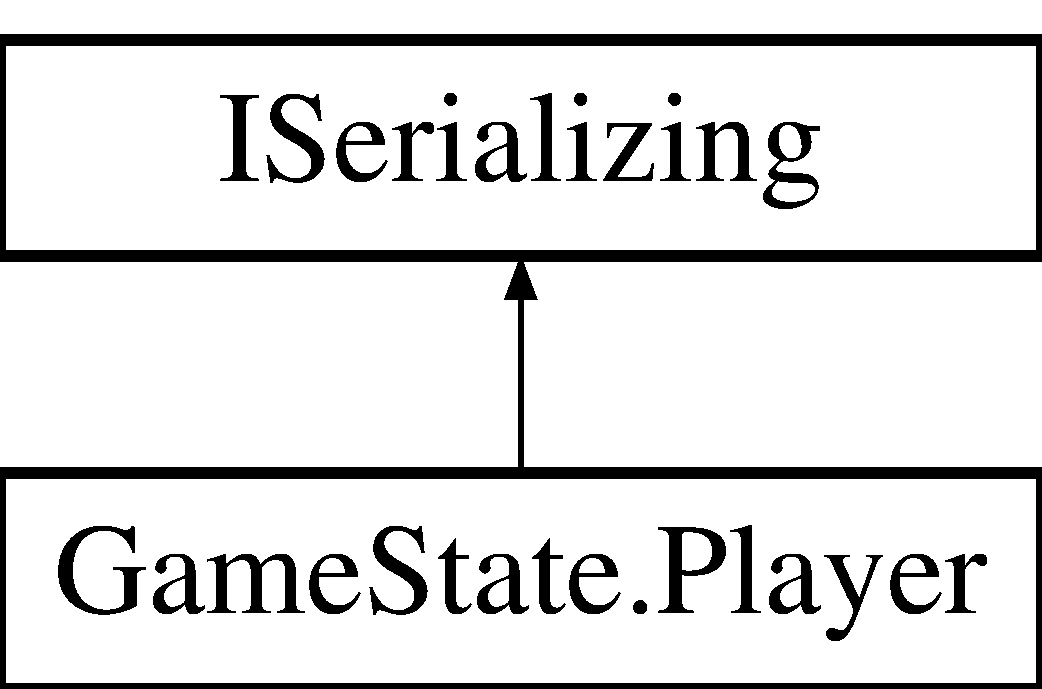
\includegraphics[height=2.000000cm]{class_game_state_1_1_player}
\end{center}
\end{figure}
\subsection*{Public Types}
\begin{DoxyCompactItemize}
\item 
enum \hyperlink{class_game_state_1_1_player_a9f54c5eca1e60acbaa2074e981f51615}{Enum\-Battle\-Selection} \{ {\bfseries A\-T\-T\-A\-C\-K}, 
{\bfseries S\-W\-A\-P}, 
{\bfseries F\-L\-E\-E}
 \}
\begin{DoxyCompactList}\small\item\em Options of types of battle moves. \end{DoxyCompactList}\end{DoxyCompactItemize}
\subsection*{Public Member Functions}
\begin{DoxyCompactItemize}
\item 
void \hyperlink{class_game_state_1_1_player_ace7e3625cf1996b8c56bcafae36673af}{copy\-From\-Game\-State} (\hyperlink{class_game_state_1_1_player}{Player} info, float delta\-Time)
\begin{DoxyCompactList}\small\item\em Copy data from a deserialized player state into this player state \end{DoxyCompactList}\item 
void \hyperlink{class_game_state_1_1_player_a59ac624b5378e8253ac70d827febfe6a}{integrate\-Physics} (float delta\-Time)
\begin{DoxyCompactList}\small\item\em Integrate physics in this object (accelleration-\/$>$velocity, velocity-\/$>$position). \end{DoxyCompactList}\item 
\hypertarget{class_game_state_1_1_player_a3ab6c2f1d15057b161ba0cba271fd9d3}{int {\bfseries Index\-Of} (\hyperlink{class_monster_data_object}{Monster\-Data\-Object} item)}\label{class_game_state_1_1_player_a3ab6c2f1d15057b161ba0cba271fd9d3}

\item 
\hypertarget{class_game_state_1_1_player_a84cdeefa239fade5ab90b42b3d55bda8}{void {\bfseries Insert} (int index, \hyperlink{class_monster_data_object}{Monster\-Data\-Object} item)}\label{class_game_state_1_1_player_a84cdeefa239fade5ab90b42b3d55bda8}

\item 
\hypertarget{class_game_state_1_1_player_a971bad69d0ef56fbd860c71ed1b56dae}{void {\bfseries Remove\-At} (int index)}\label{class_game_state_1_1_player_a971bad69d0ef56fbd860c71ed1b56dae}

\item 
\hypertarget{class_game_state_1_1_player_ad791ddd2f697e5237c6e04c7fc5c1e5f}{void {\bfseries Add} (\hyperlink{class_monster_data_object}{Monster\-Data\-Object} item)}\label{class_game_state_1_1_player_ad791ddd2f697e5237c6e04c7fc5c1e5f}

\item 
\hypertarget{class_game_state_1_1_player_a732e5b36f28a1fa3aa998fb5659a986a}{void {\bfseries Clear} ()}\label{class_game_state_1_1_player_a732e5b36f28a1fa3aa998fb5659a986a}

\item 
\hypertarget{class_game_state_1_1_player_ac862c1353bfbc38d53e2301548ded23a}{bool {\bfseries Contains} (\hyperlink{class_monster_data_object}{Monster\-Data\-Object} item)}\label{class_game_state_1_1_player_ac862c1353bfbc38d53e2301548ded23a}

\item 
\hypertarget{class_game_state_1_1_player_a5c3546baf67a5d27553c814df4def68a}{void {\bfseries Copy\-To} (\hyperlink{class_monster_data_object}{Monster\-Data\-Object}\mbox{[}$\,$\mbox{]} array, int array\-Index)}\label{class_game_state_1_1_player_a5c3546baf67a5d27553c814df4def68a}

\item 
\hypertarget{class_game_state_1_1_player_a98c86c2ffe06038710acb4951479dff9}{bool {\bfseries Remove} (\hyperlink{class_monster_data_object}{Monster\-Data\-Object} item)}\label{class_game_state_1_1_player_a98c86c2ffe06038710acb4951479dff9}

\item 
\hypertarget{class_game_state_1_1_player_a02e1f98267c1fcf0258528ad72bd5d25}{I\-Enumerator$<$ \hyperlink{class_monster_data_object}{Monster\-Data\-Object} $>$ {\bfseries Get\-Enumerator} ()}\label{class_game_state_1_1_player_a02e1f98267c1fcf0258528ad72bd5d25}

\item 
\hypertarget{class_game_state_1_1_player_abb92c259431397bdda45f001e59addea}{int \hyperlink{class_game_state_1_1_player_abb92c259431397bdda45f001e59addea}{get\-Size} () const }\label{class_game_state_1_1_player_abb92c259431397bdda45f001e59addea}

\begin{DoxyCompactList}\small\item\em The maximum length of the \hyperlink{class_game_state_1_1_player}{Player} when serialized into a byte\mbox{[}\mbox{]}. \end{DoxyCompactList}\end{DoxyCompactItemize}
\subsection*{Public Attributes}
\begin{DoxyCompactItemize}
\item 
I\-D \hyperlink{class_game_state_1_1_player_aacc123df8ea5256f83c1060a5fdd19c2}{client\-I\-D}
\begin{DoxyCompactList}\small\item\em A unique identifier of the client which controls this player. Unqiue across all peers in the network. \end{DoxyCompactList}\item 
I\-D \hyperlink{class_game_state_1_1_player_acbd28d89e6eb8611aa66452ec31e9133}{player\-I\-D}
\begin{DoxyCompactList}\small\item\em A unique identifier of the player object. Unique across all peers in the network. \end{DoxyCompactList}\item 
I\-D \hyperlink{class_game_state_1_1_player_ae0383475b3348fb85ba5be64433443ff}{local\-I\-D}
\begin{DoxyCompactList}\small\item\em A unique identifier of the player object in a local context. Unique across all players with the same \hyperlink{class_game_state_1_1_player_aacc123df8ea5256f83c1060a5fdd19c2}{client\-I\-D}. \end{DoxyCompactList}\item 
string \hyperlink{class_game_state_1_1_player_afc2b145df544ca5bffc7c87ef294bcde}{name}
\begin{DoxyCompactList}\small\item\em The name identifier of the player. Not unique. Enforced max of \hyperlink{class_game_state_1_1_player_a1cdc9de8183b220e87632f7f6a7147d0}{S\-I\-Z\-E\-\_\-\-M\-A\-X\-\_\-\-N\-A\-M\-E}. \end{DoxyCompactList}\item 
Color \hyperlink{class_game_state_1_1_player_a38366fae101c03655d90443f174e362d}{color}
\begin{DoxyCompactList}\small\item\em The color-\/overlay. \end{DoxyCompactList}\item 
Vector3 \hyperlink{class_game_state_1_1_player_a24a9ccd0325cae667f125821b3be79c2}{position}
\begin{DoxyCompactList}\small\item\em The position of the player in the open-\/world. \end{DoxyCompactList}\item 
Vector3 \hyperlink{class_game_state_1_1_player_aa22122c85cfdae428d82bd1571ab022a}{velocity}
\begin{DoxyCompactList}\small\item\em The velocity of the player in the open-\/world. \end{DoxyCompactList}\item 
Vector3 \hyperlink{class_game_state_1_1_player_a8f25769e000454ef477d359f44a5ed31}{accelleration}
\begin{DoxyCompactList}\small\item\em The accelleration of the player in the open-\/world. \end{DoxyCompactList}\item 
bool \hyperlink{class_game_state_1_1_player_a3cff343fceb3dc315d2371fc8fe25ec6}{in\-Battle}
\begin{DoxyCompactList}\small\item\em If the player is presently in a battle with a player or A\-I. \end{DoxyCompactList}\item 
I\-D \hyperlink{class_game_state_1_1_player_aaed188c94b7f6be4dabe39744aa818ca}{player\-I\-D\-Opponent}
\begin{DoxyCompactList}\small\item\em The player I\-D of the opponent. Could be irrelevant if player is in local battle with A\-I. \end{DoxyCompactList}\item 
\hyperlink{class_game_state_1_1_player_a9f54c5eca1e60acbaa2074e981f51615}{Enum\-Battle\-Selection} \hyperlink{class_game_state_1_1_player_a123c8ee2ef6e66e88bcca1a80f73ab4a}{battle\-Selection}
\begin{DoxyCompactList}\small\item\em The type of action the player makes in battle. \end{DoxyCompactList}\item 
int \hyperlink{class_game_state_1_1_player_a3bfa8ea6e2067982474dc4f6073061c5}{battle\-Choice}
\begin{DoxyCompactList}\small\item\em The descriptor for the type of action (narrows down choice to options like which attack a cretin makes, or what cretin is being swapped to). \end{DoxyCompactList}\item 
uint \hyperlink{class_game_state_1_1_player_a3a4d13459cad9bd58e058ddc6387af70}{wins}
\begin{DoxyCompactList}\small\item\em The total number of wins since entering the server. \end{DoxyCompactList}\item 
uint \hyperlink{class_game_state_1_1_player_a6cf0778cc27a824eac211b8b29b3dfcc}{rank}
\begin{DoxyCompactList}\small\item\em The rank of the player in the scoreboard. The higher \hyperlink{class_game_state_1_1_player_a3a4d13459cad9bd58e058ddc6387af70}{wins} is compared to other players, the \end{DoxyCompactList}\item 
List$<$ uint $>$ \hyperlink{class_game_state_1_1_player_a2c4ed3c60a2969cd4f891e12c8265377}{monster\-I\-Ds}
\begin{DoxyCompactList}\small\item\em A list of all the cretins the player has. \end{DoxyCompactList}\item 
\hyperlink{class_player_reference}{Player\-Reference} \hyperlink{class_game_state_1_1_player_aebf24de01e14055dc940d0493753484f}{object\-Reference}
\begin{DoxyCompactList}\small\item\em The reference to the Game\-Object in the local unity instance \end{DoxyCompactList}\item 
Render\-Texture \hyperlink{class_game_state_1_1_player_ac1f7e0b5bc335c32c3be71e3653787a6}{camera\-Texture}
\begin{DoxyCompactList}\small\item\em Reference to the render output for this \hyperlink{class_game_state_1_1_player_aebf24de01e14055dc940d0493753484f}{object\-Reference} \end{DoxyCompactList}\item 
\hypertarget{class_game_state_1_1_player_a1bef4cd92306bd5cf330c4756e63686c}{unsigned int \hyperlink{class_game_state_1_1_player_a1bef4cd92306bd5cf330c4756e63686c}{client\-I\-D}}\label{class_game_state_1_1_player_a1bef4cd92306bd5cf330c4756e63686c}

\begin{DoxyCompactList}\small\item\em The client\-I\-D of the controlling client. This is unique across all peers in a network. \end{DoxyCompactList}\item 
\hypertarget{class_game_state_1_1_player_ac71d68698435ee1c625237b1f2b377cb}{unsigned int \hyperlink{class_game_state_1_1_player_ac71d68698435ee1c625237b1f2b377cb}{player\-I\-D}}\label{class_game_state_1_1_player_ac71d68698435ee1c625237b1f2b377cb}

\begin{DoxyCompactList}\small\item\em The player\-I\-D of the character. This is unique across all players in a network. \end{DoxyCompactList}\item 
\hypertarget{class_game_state_1_1_player_ab1600ee9b9d01027e5304e991be11407}{unsigned int \hyperlink{class_game_state_1_1_player_ab1600ee9b9d01027e5304e991be11407}{local\-I\-D}}\label{class_game_state_1_1_player_ab1600ee9b9d01027e5304e991be11407}

\begin{DoxyCompactList}\small\item\em The local\-I\-D of the character. This is unqiue to all players with the same \hyperlink{class_game_state_1_1_player_aacc123df8ea5256f83c1060a5fdd19c2}{Player\-::client\-I\-D}. \end{DoxyCompactList}\item 
\hypertarget{class_game_state_1_1_player_a6638478952037ab0d1b3b0a3c496a820}{std\-::string \hyperlink{class_game_state_1_1_player_a6638478952037ab0d1b3b0a3c496a820}{name}}\label{class_game_state_1_1_player_a6638478952037ab0d1b3b0a3c496a820}

\begin{DoxyCompactList}\small\item\em the name of the character \end{DoxyCompactList}\item 
\hypertarget{class_game_state_1_1_player_a54b350ee750dd994b421ad4332448112}{float \hyperlink{class_game_state_1_1_player_a54b350ee750dd994b421ad4332448112}{color\-R}}\label{class_game_state_1_1_player_a54b350ee750dd994b421ad4332448112}

\begin{DoxyCompactList}\small\item\em the highlight color of the character \end{DoxyCompactList}\item 
\hypertarget{class_game_state_1_1_player_a26c9551e961a1f601fd689f3677ce277}{float {\bfseries color\-G}}\label{class_game_state_1_1_player_a26c9551e961a1f601fd689f3677ce277}

\item 
\hypertarget{class_game_state_1_1_player_ad3f992ed5676471f80c6ba3c9ce0f505}{float {\bfseries color\-B}}\label{class_game_state_1_1_player_ad3f992ed5676471f80c6ba3c9ce0f505}

\item 
\hypertarget{class_game_state_1_1_player_a828e830d7461991e4980f7fc7336e552}{float {\bfseries color\-A}}\label{class_game_state_1_1_player_a828e830d7461991e4980f7fc7336e552}

\item 
\hypertarget{class_game_state_1_1_player_a0342f6d74f9c08351cd0c5139ac55de6}{float \hyperlink{class_game_state_1_1_player_a0342f6d74f9c08351cd0c5139ac55de6}{pos\-X}}\label{class_game_state_1_1_player_a0342f6d74f9c08351cd0c5139ac55de6}

\begin{DoxyCompactList}\small\item\em the position \end{DoxyCompactList}\item 
\hypertarget{class_game_state_1_1_player_a831daac1ac1f3da9ec90a9c2247b3b2f}{float {\bfseries pos\-Y}}\label{class_game_state_1_1_player_a831daac1ac1f3da9ec90a9c2247b3b2f}

\item 
\hypertarget{class_game_state_1_1_player_af71e7ca3fb57c91895254d8c2741a36b}{float {\bfseries pos\-Z}}\label{class_game_state_1_1_player_af71e7ca3fb57c91895254d8c2741a36b}

\item 
\hypertarget{class_game_state_1_1_player_afcc72f7f23db9714a20ac1b08fda0288}{float \hyperlink{class_game_state_1_1_player_afcc72f7f23db9714a20ac1b08fda0288}{vel\-X}}\label{class_game_state_1_1_player_afcc72f7f23db9714a20ac1b08fda0288}

\begin{DoxyCompactList}\small\item\em velocity \end{DoxyCompactList}\item 
\hypertarget{class_game_state_1_1_player_a9e5fa5186567b76be447afe96e86c9f9}{float {\bfseries vel\-Y}}\label{class_game_state_1_1_player_a9e5fa5186567b76be447afe96e86c9f9}

\item 
\hypertarget{class_game_state_1_1_player_af69e80093c2205d374bfcab9baa3f57c}{float {\bfseries vel\-Z}}\label{class_game_state_1_1_player_af69e80093c2205d374bfcab9baa3f57c}

\item 
\hypertarget{class_game_state_1_1_player_a0d726c8aaa2bb433e9d6d3e09c945328}{float \hyperlink{class_game_state_1_1_player_a0d726c8aaa2bb433e9d6d3e09c945328}{acc\-X}}\label{class_game_state_1_1_player_a0d726c8aaa2bb433e9d6d3e09c945328}

\begin{DoxyCompactList}\small\item\em and acceleration \end{DoxyCompactList}\item 
\hypertarget{class_game_state_1_1_player_a13a126f3ac6426ce52effd7ccd14c5f0}{float {\bfseries acc\-Y}}\label{class_game_state_1_1_player_a13a126f3ac6426ce52effd7ccd14c5f0}

\item 
\hypertarget{class_game_state_1_1_player_abec98fdec68ed34c3ff6bf202d4ac446}{float {\bfseries acc\-Z}}\label{class_game_state_1_1_player_abec98fdec68ed34c3ff6bf202d4ac446}

\item 
\hypertarget{class_game_state_1_1_player_aac7333a06ea194848f12090be762cdd6}{unsigned int \hyperlink{class_game_state_1_1_player_aac7333a06ea194848f12090be762cdd6}{wins}}\label{class_game_state_1_1_player_aac7333a06ea194848f12090be762cdd6}

\begin{DoxyCompactList}\small\item\em Number of wins the player has. \end{DoxyCompactList}\item 
\hypertarget{class_game_state_1_1_player_a43dd8a9e79c35d9615596fb6ab25d653}{unsigned int \hyperlink{class_game_state_1_1_player_a43dd8a9e79c35d9615596fb6ab25d653}{rank}}\label{class_game_state_1_1_player_a43dd8a9e79c35d9615596fb6ab25d653}

\begin{DoxyCompactList}\small\item\em Rank of player on the scoreboard. \end{DoxyCompactList}\item 
\hypertarget{class_game_state_1_1_player_a7f5bbae042c927e8dd0f27a189a18dea}{int {\bfseries monsters\-Count}}\label{class_game_state_1_1_player_a7f5bbae042c927e8dd0f27a189a18dea}

\item 
\hypertarget{class_game_state_1_1_player_a2cc3642e98d820c6e4fce5864254c79e}{unsigned int $\ast$ {\bfseries monsters}}\label{class_game_state_1_1_player_a2cc3642e98d820c6e4fce5864254c79e}

\item 
\hypertarget{class_game_state_1_1_player_ae60a4f411ef984c6d649d98c65b274bd}{int \hyperlink{class_game_state_1_1_player_ae60a4f411ef984c6d649d98c65b274bd}{battle\-Opponent\-Id}}\label{class_game_state_1_1_player_ae60a4f411ef984c6d649d98c65b274bd}

\begin{DoxyCompactList}\small\item\em the player\-Id of the opponent, -\/1 if invalid, otherwise $>$= 0 \end{DoxyCompactList}\item 
\hypertarget{class_game_state_1_1_player_a2383ab7d3783c5122f3e68230069eb2e}{int \hyperlink{class_game_state_1_1_player_a2383ab7d3783c5122f3e68230069eb2e}{last\-Battle\-Selection}}\label{class_game_state_1_1_player_a2383ab7d3783c5122f3e68230069eb2e}

\begin{DoxyCompactList}\small\item\em the last selection in battles, -\/1 if invalid, otherwise $>$= 0 \end{DoxyCompactList}\item 
\hypertarget{class_game_state_1_1_player_adf61e3258c2170b7b66355389cca541f}{int \hyperlink{class_game_state_1_1_player_adf61e3258c2170b7b66355389cca541f}{last\-Battle\-Choice}}\label{class_game_state_1_1_player_adf61e3258c2170b7b66355389cca541f}

\begin{DoxyCompactList}\small\item\em the last selection choice in battle, -\/1 if invalid, otherwise $>$= 0 \end{DoxyCompactList}\end{DoxyCompactItemize}
\subsection*{Static Public Attributes}
\begin{DoxyCompactItemize}
\item 
static int \hyperlink{class_game_state_1_1_player_ada2d068d3d5f973f73abac805c162d17}{S\-I\-Z\-E}
\begin{DoxyCompactList}\small\item\em The serialized size of the \hyperlink{class_game_state_1_1_player}{Player} object \end{DoxyCompactList}\item 
static int \hyperlink{class_game_state_1_1_player_a1cdc9de8183b220e87632f7f6a7147d0}{S\-I\-Z\-E\-\_\-\-M\-A\-X\-\_\-\-N\-A\-M\-E} = 10
\begin{DoxyCompactList}\small\item\em The maximum length of \hyperlink{class_game_state_1_1_player_afc2b145df544ca5bffc7c87ef294bcde}{Game\-State.\-Player.\-name} \end{DoxyCompactList}\item 
\hypertarget{class_game_state_1_1_player_a16d0264ca6adfedb582e22f59a550fc5}{static const int \hyperlink{class_game_state_1_1_player_a16d0264ca6adfedb582e22f59a550fc5}{S\-I\-Z\-E\-\_\-\-M\-A\-X\-\_\-\-N\-A\-M\-E} = 10}\label{class_game_state_1_1_player_a16d0264ca6adfedb582e22f59a550fc5}

\begin{DoxyCompactList}\small\item\em The maximum length of any player's name. \end{DoxyCompactList}\end{DoxyCompactItemize}
\subsection*{Properties}
\begin{DoxyCompactItemize}
\item 
bool \hyperlink{class_game_state_1_1_player_affd7c601a6d763dafdc59a58c415e9e7}{is\-Local}\hspace{0.3cm}{\ttfamily  \mbox{[}get\mbox{]}}
\begin{DoxyCompactList}\small\item\em If the player id is from a local player (controlled on this game) or networked (controlled by a peer) \end{DoxyCompactList}\item 
\hypertarget{class_game_state_1_1_player_aebfa739a98ff4f88d151235905b439bf}{I\-List$<$ \hyperlink{class_monster_data_object}{Monster\-Data\-Object} $>$ {\bfseries monsters}\hspace{0.3cm}{\ttfamily  \mbox{[}get\mbox{]}}}\label{class_game_state_1_1_player_aebfa739a98ff4f88d151235905b439bf}

\item 
\hypertarget{class_game_state_1_1_player_ab8dafc199bbda42740ab5f3587202495}{\hyperlink{class_monster_data_object}{Monster\-Data\-Object} {\bfseries this\mbox{[}int index\mbox{]}}\hspace{0.3cm}{\ttfamily  \mbox{[}get, set\mbox{]}}}\label{class_game_state_1_1_player_ab8dafc199bbda42740ab5f3587202495}

\end{DoxyCompactItemize}


\subsection{Detailed Description}
A state class for all \hyperlink{class_game_state_1_1_player}{Player} objects 

A structure to hold information about each player.

\subsection{Member Enumeration Documentation}
\hypertarget{class_game_state_1_1_player_a9f54c5eca1e60acbaa2074e981f51615}{\index{Game\-State\-::\-Player@{Game\-State\-::\-Player}!Enum\-Battle\-Selection@{Enum\-Battle\-Selection}}
\index{Enum\-Battle\-Selection@{Enum\-Battle\-Selection}!GameState::Player@{Game\-State\-::\-Player}}
\subsubsection[{Enum\-Battle\-Selection}]{\setlength{\rightskip}{0pt plus 5cm}enum {\bf Game\-State.\-Player.\-Enum\-Battle\-Selection}}}\label{class_game_state_1_1_player_a9f54c5eca1e60acbaa2074e981f51615}


Options of types of battle moves. 



\subsection{Member Function Documentation}
\hypertarget{class_game_state_1_1_player_ace7e3625cf1996b8c56bcafae36673af}{\index{Game\-State\-::\-Player@{Game\-State\-::\-Player}!copy\-From\-Game\-State@{copy\-From\-Game\-State}}
\index{copy\-From\-Game\-State@{copy\-From\-Game\-State}!GameState::Player@{Game\-State\-::\-Player}}
\subsubsection[{copy\-From\-Game\-State}]{\setlength{\rightskip}{0pt plus 5cm}void Game\-State.\-Player.\-copy\-From\-Game\-State (
\begin{DoxyParamCaption}
\item[{{\bf Player}}]{info, }
\item[{float}]{delta\-Time}
\end{DoxyParamCaption}
)\hspace{0.3cm}{\ttfamily [inline]}}}\label{class_game_state_1_1_player_ace7e3625cf1996b8c56bcafae36673af}


Copy data from a deserialized player state into this player state 


\begin{DoxyParams}{Parameters}
{\em info} & The newly deserialized player state.\\
\hline
{\em delta\-Time} & The time to integrate physics over.\\
\hline
\end{DoxyParams}
\hypertarget{class_game_state_1_1_player_a59ac624b5378e8253ac70d827febfe6a}{\index{Game\-State\-::\-Player@{Game\-State\-::\-Player}!integrate\-Physics@{integrate\-Physics}}
\index{integrate\-Physics@{integrate\-Physics}!GameState::Player@{Game\-State\-::\-Player}}
\subsubsection[{integrate\-Physics}]{\setlength{\rightskip}{0pt plus 5cm}void Game\-State.\-Player.\-integrate\-Physics (
\begin{DoxyParamCaption}
\item[{float}]{delta\-Time}
\end{DoxyParamCaption}
)\hspace{0.3cm}{\ttfamily [inline]}}}\label{class_game_state_1_1_player_a59ac624b5378e8253ac70d827febfe6a}


Integrate physics in this object (accelleration-\/$>$velocity, velocity-\/$>$position). 


\begin{DoxyParams}{Parameters}
{\em delta\-Time} & The time to integrate over.\\
\hline
\end{DoxyParams}


\subsection{Member Data Documentation}
\hypertarget{class_game_state_1_1_player_a8f25769e000454ef477d359f44a5ed31}{\index{Game\-State\-::\-Player@{Game\-State\-::\-Player}!accelleration@{accelleration}}
\index{accelleration@{accelleration}!GameState::Player@{Game\-State\-::\-Player}}
\subsubsection[{accelleration}]{\setlength{\rightskip}{0pt plus 5cm}Vector3 Game\-State.\-Player.\-accelleration}}\label{class_game_state_1_1_player_a8f25769e000454ef477d359f44a5ed31}


The accelleration of the player in the open-\/world. 

\hypertarget{class_game_state_1_1_player_a3bfa8ea6e2067982474dc4f6073061c5}{\index{Game\-State\-::\-Player@{Game\-State\-::\-Player}!battle\-Choice@{battle\-Choice}}
\index{battle\-Choice@{battle\-Choice}!GameState::Player@{Game\-State\-::\-Player}}
\subsubsection[{battle\-Choice}]{\setlength{\rightskip}{0pt plus 5cm}int Game\-State.\-Player.\-battle\-Choice}}\label{class_game_state_1_1_player_a3bfa8ea6e2067982474dc4f6073061c5}


The descriptor for the type of action (narrows down choice to options like which attack a cretin makes, or what cretin is being swapped to). 

\hypertarget{class_game_state_1_1_player_a123c8ee2ef6e66e88bcca1a80f73ab4a}{\index{Game\-State\-::\-Player@{Game\-State\-::\-Player}!battle\-Selection@{battle\-Selection}}
\index{battle\-Selection@{battle\-Selection}!GameState::Player@{Game\-State\-::\-Player}}
\subsubsection[{battle\-Selection}]{\setlength{\rightskip}{0pt plus 5cm}{\bf Enum\-Battle\-Selection} Game\-State.\-Player.\-battle\-Selection}}\label{class_game_state_1_1_player_a123c8ee2ef6e66e88bcca1a80f73ab4a}


The type of action the player makes in battle. 

\hypertarget{class_game_state_1_1_player_ac1f7e0b5bc335c32c3be71e3653787a6}{\index{Game\-State\-::\-Player@{Game\-State\-::\-Player}!camera\-Texture@{camera\-Texture}}
\index{camera\-Texture@{camera\-Texture}!GameState::Player@{Game\-State\-::\-Player}}
\subsubsection[{camera\-Texture}]{\setlength{\rightskip}{0pt plus 5cm}Render\-Texture Game\-State.\-Player.\-camera\-Texture}}\label{class_game_state_1_1_player_ac1f7e0b5bc335c32c3be71e3653787a6}


Reference to the render output for this \hyperlink{class_game_state_1_1_player_aebf24de01e14055dc940d0493753484f}{object\-Reference} 

\hypertarget{class_game_state_1_1_player_aacc123df8ea5256f83c1060a5fdd19c2}{\index{Game\-State\-::\-Player@{Game\-State\-::\-Player}!client\-I\-D@{client\-I\-D}}
\index{client\-I\-D@{client\-I\-D}!GameState::Player@{Game\-State\-::\-Player}}
\subsubsection[{client\-I\-D}]{\setlength{\rightskip}{0pt plus 5cm}I\-D Game\-State.\-Player.\-client\-I\-D}}\label{class_game_state_1_1_player_aacc123df8ea5256f83c1060a5fdd19c2}


A unique identifier of the client which controls this player. Unqiue across all peers in the network. 

\hypertarget{class_game_state_1_1_player_a38366fae101c03655d90443f174e362d}{\index{Game\-State\-::\-Player@{Game\-State\-::\-Player}!color@{color}}
\index{color@{color}!GameState::Player@{Game\-State\-::\-Player}}
\subsubsection[{color}]{\setlength{\rightskip}{0pt plus 5cm}Color Game\-State.\-Player.\-color}}\label{class_game_state_1_1_player_a38366fae101c03655d90443f174e362d}


The color-\/overlay. 

\hypertarget{class_game_state_1_1_player_a3cff343fceb3dc315d2371fc8fe25ec6}{\index{Game\-State\-::\-Player@{Game\-State\-::\-Player}!in\-Battle@{in\-Battle}}
\index{in\-Battle@{in\-Battle}!GameState::Player@{Game\-State\-::\-Player}}
\subsubsection[{in\-Battle}]{\setlength{\rightskip}{0pt plus 5cm}bool Game\-State.\-Player.\-in\-Battle}}\label{class_game_state_1_1_player_a3cff343fceb3dc315d2371fc8fe25ec6}


If the player is presently in a battle with a player or A\-I. 

if the player is in battle\hypertarget{class_game_state_1_1_player_ae0383475b3348fb85ba5be64433443ff}{\index{Game\-State\-::\-Player@{Game\-State\-::\-Player}!local\-I\-D@{local\-I\-D}}
\index{local\-I\-D@{local\-I\-D}!GameState::Player@{Game\-State\-::\-Player}}
\subsubsection[{local\-I\-D}]{\setlength{\rightskip}{0pt plus 5cm}I\-D Game\-State.\-Player.\-local\-I\-D}}\label{class_game_state_1_1_player_ae0383475b3348fb85ba5be64433443ff}


A unique identifier of the player object in a local context. Unique across all players with the same \hyperlink{class_game_state_1_1_player_aacc123df8ea5256f83c1060a5fdd19c2}{client\-I\-D}. 

\hypertarget{class_game_state_1_1_player_a2c4ed3c60a2969cd4f891e12c8265377}{\index{Game\-State\-::\-Player@{Game\-State\-::\-Player}!monster\-I\-Ds@{monster\-I\-Ds}}
\index{monster\-I\-Ds@{monster\-I\-Ds}!GameState::Player@{Game\-State\-::\-Player}}
\subsubsection[{monster\-I\-Ds}]{\setlength{\rightskip}{0pt plus 5cm}List$<$uint$>$ Game\-State.\-Player.\-monster\-I\-Ds}}\label{class_game_state_1_1_player_a2c4ed3c60a2969cd4f891e12c8265377}


A list of all the cretins the player has. 

\hypertarget{class_game_state_1_1_player_afc2b145df544ca5bffc7c87ef294bcde}{\index{Game\-State\-::\-Player@{Game\-State\-::\-Player}!name@{name}}
\index{name@{name}!GameState::Player@{Game\-State\-::\-Player}}
\subsubsection[{name}]{\setlength{\rightskip}{0pt plus 5cm}string Game\-State.\-Player.\-name}}\label{class_game_state_1_1_player_afc2b145df544ca5bffc7c87ef294bcde}


The name identifier of the player. Not unique. Enforced max of \hyperlink{class_game_state_1_1_player_a1cdc9de8183b220e87632f7f6a7147d0}{S\-I\-Z\-E\-\_\-\-M\-A\-X\-\_\-\-N\-A\-M\-E}. 

\hypertarget{class_game_state_1_1_player_aebf24de01e14055dc940d0493753484f}{\index{Game\-State\-::\-Player@{Game\-State\-::\-Player}!object\-Reference@{object\-Reference}}
\index{object\-Reference@{object\-Reference}!GameState::Player@{Game\-State\-::\-Player}}
\subsubsection[{object\-Reference}]{\setlength{\rightskip}{0pt plus 5cm}{\bf Player\-Reference} Game\-State.\-Player.\-object\-Reference}}\label{class_game_state_1_1_player_aebf24de01e14055dc940d0493753484f}


The reference to the Game\-Object in the local unity instance 

\hypertarget{class_game_state_1_1_player_acbd28d89e6eb8611aa66452ec31e9133}{\index{Game\-State\-::\-Player@{Game\-State\-::\-Player}!player\-I\-D@{player\-I\-D}}
\index{player\-I\-D@{player\-I\-D}!GameState::Player@{Game\-State\-::\-Player}}
\subsubsection[{player\-I\-D}]{\setlength{\rightskip}{0pt plus 5cm}I\-D Game\-State.\-Player.\-player\-I\-D}}\label{class_game_state_1_1_player_acbd28d89e6eb8611aa66452ec31e9133}


A unique identifier of the player object. Unique across all peers in the network. 

\hypertarget{class_game_state_1_1_player_aaed188c94b7f6be4dabe39744aa818ca}{\index{Game\-State\-::\-Player@{Game\-State\-::\-Player}!player\-I\-D\-Opponent@{player\-I\-D\-Opponent}}
\index{player\-I\-D\-Opponent@{player\-I\-D\-Opponent}!GameState::Player@{Game\-State\-::\-Player}}
\subsubsection[{player\-I\-D\-Opponent}]{\setlength{\rightskip}{0pt plus 5cm}I\-D Game\-State.\-Player.\-player\-I\-D\-Opponent}}\label{class_game_state_1_1_player_aaed188c94b7f6be4dabe39744aa818ca}


The player I\-D of the opponent. Could be irrelevant if player is in local battle with A\-I. 

\hypertarget{class_game_state_1_1_player_a24a9ccd0325cae667f125821b3be79c2}{\index{Game\-State\-::\-Player@{Game\-State\-::\-Player}!position@{position}}
\index{position@{position}!GameState::Player@{Game\-State\-::\-Player}}
\subsubsection[{position}]{\setlength{\rightskip}{0pt plus 5cm}Vector3 Game\-State.\-Player.\-position}}\label{class_game_state_1_1_player_a24a9ccd0325cae667f125821b3be79c2}


The position of the player in the open-\/world. 

\hypertarget{class_game_state_1_1_player_a6cf0778cc27a824eac211b8b29b3dfcc}{\index{Game\-State\-::\-Player@{Game\-State\-::\-Player}!rank@{rank}}
\index{rank@{rank}!GameState::Player@{Game\-State\-::\-Player}}
\subsubsection[{rank}]{\setlength{\rightskip}{0pt plus 5cm}uint Game\-State.\-Player.\-rank}}\label{class_game_state_1_1_player_a6cf0778cc27a824eac211b8b29b3dfcc}


The rank of the player in the scoreboard. The higher \hyperlink{class_game_state_1_1_player_a3a4d13459cad9bd58e058ddc6387af70}{wins} is compared to other players, the 

\hypertarget{class_game_state_1_1_player_ada2d068d3d5f973f73abac805c162d17}{\index{Game\-State\-::\-Player@{Game\-State\-::\-Player}!S\-I\-Z\-E@{S\-I\-Z\-E}}
\index{S\-I\-Z\-E@{S\-I\-Z\-E}!GameState::Player@{Game\-State\-::\-Player}}
\subsubsection[{S\-I\-Z\-E}]{\setlength{\rightskip}{0pt plus 5cm}int Game\-State.\-Player.\-S\-I\-Z\-E\hspace{0.3cm}{\ttfamily [static]}}}\label{class_game_state_1_1_player_ada2d068d3d5f973f73abac805c162d17}
{\bfseries Initial value\-:}
\begin{DoxyCode}
=
            \textcolor{keyword}{sizeof}(ID) 
            + \textcolor{keyword}{sizeof}(ID) 
            + \textcolor{keyword}{sizeof}(ID) 
            + \textcolor{keyword}{sizeof}(\textcolor{keywordtype}{int}) + (\hyperlink{class_game_state_1_1_player_a1cdc9de8183b220e87632f7f6a7147d0}{SIZE\_MAX\_NAME} * \textcolor{keyword}{sizeof}(char))
            + (\textcolor{keyword}{sizeof}(float) * 3) 
            + (\textcolor{keyword}{sizeof}(float) * 3) 
            + (\textcolor{keyword}{sizeof}(float) * 3) 
            + (\textcolor{keyword}{sizeof}(float) * 3) 
            + \textcolor{keyword}{sizeof}(bool) 
            + \textcolor{keyword}{sizeof}(uint) 
            + \textcolor{keyword}{sizeof}(uint)
\end{DoxyCode}


The serialized size of the \hyperlink{class_game_state_1_1_player}{Player} object 

\hypertarget{class_game_state_1_1_player_a1cdc9de8183b220e87632f7f6a7147d0}{\index{Game\-State\-::\-Player@{Game\-State\-::\-Player}!S\-I\-Z\-E\-\_\-\-M\-A\-X\-\_\-\-N\-A\-M\-E@{S\-I\-Z\-E\-\_\-\-M\-A\-X\-\_\-\-N\-A\-M\-E}}
\index{S\-I\-Z\-E\-\_\-\-M\-A\-X\-\_\-\-N\-A\-M\-E@{S\-I\-Z\-E\-\_\-\-M\-A\-X\-\_\-\-N\-A\-M\-E}!GameState::Player@{Game\-State\-::\-Player}}
\subsubsection[{S\-I\-Z\-E\-\_\-\-M\-A\-X\-\_\-\-N\-A\-M\-E}]{\setlength{\rightskip}{0pt plus 5cm}int Game\-State.\-Player.\-S\-I\-Z\-E\-\_\-\-M\-A\-X\-\_\-\-N\-A\-M\-E = 10\hspace{0.3cm}{\ttfamily [static]}}}\label{class_game_state_1_1_player_a1cdc9de8183b220e87632f7f6a7147d0}


The maximum length of \hyperlink{class_game_state_1_1_player_afc2b145df544ca5bffc7c87ef294bcde}{Game\-State.\-Player.\-name} 

\hypertarget{class_game_state_1_1_player_aa22122c85cfdae428d82bd1571ab022a}{\index{Game\-State\-::\-Player@{Game\-State\-::\-Player}!velocity@{velocity}}
\index{velocity@{velocity}!GameState::Player@{Game\-State\-::\-Player}}
\subsubsection[{velocity}]{\setlength{\rightskip}{0pt plus 5cm}Vector3 Game\-State.\-Player.\-velocity}}\label{class_game_state_1_1_player_aa22122c85cfdae428d82bd1571ab022a}


The velocity of the player in the open-\/world. 

\hypertarget{class_game_state_1_1_player_a3a4d13459cad9bd58e058ddc6387af70}{\index{Game\-State\-::\-Player@{Game\-State\-::\-Player}!wins@{wins}}
\index{wins@{wins}!GameState::Player@{Game\-State\-::\-Player}}
\subsubsection[{wins}]{\setlength{\rightskip}{0pt plus 5cm}uint Game\-State.\-Player.\-wins}}\label{class_game_state_1_1_player_a3a4d13459cad9bd58e058ddc6387af70}


The total number of wins since entering the server. 



\subsection{Property Documentation}
\hypertarget{class_game_state_1_1_player_affd7c601a6d763dafdc59a58c415e9e7}{\index{Game\-State\-::\-Player@{Game\-State\-::\-Player}!is\-Local@{is\-Local}}
\index{is\-Local@{is\-Local}!GameState::Player@{Game\-State\-::\-Player}}
\subsubsection[{is\-Local}]{\setlength{\rightskip}{0pt plus 5cm}bool Game\-State.\-Player.\-is\-Local\hspace{0.3cm}{\ttfamily [get]}}}\label{class_game_state_1_1_player_affd7c601a6d763dafdc59a58c415e9e7}


If the player id is from a local player (controlled on this game) or networked (controlled by a peer) 



The documentation for this struct was generated from the following files\-:\begin{DoxyCompactItemize}
\item 
/home/travis/build/temportalflux/\-Champ\-Net/\-Unity/\-Assets/\-Scripts/Game\-State.\-cs\item 
/home/travis/build/temportalflux/\-Champ\-Net/\-Champ\-Net/\-Champ\-Net\-Plugin\-Test/include/Game\-State.\-h\item 
/home/travis/build/temportalflux/\-Champ\-Net/\-Champ\-Net/\-Champ\-Net\-Plugin\-Test/source/Game\-State.\-cpp\end{DoxyCompactItemize}

\hypertarget{class_player_character_controller}{\section{Player\-Character\-Controller Class Reference}
\label{class_player_character_controller}\index{Player\-Character\-Controller@{Player\-Character\-Controller}}
}
Inheritance diagram for Player\-Character\-Controller\-:\begin{figure}[H]
\begin{center}
\leavevmode
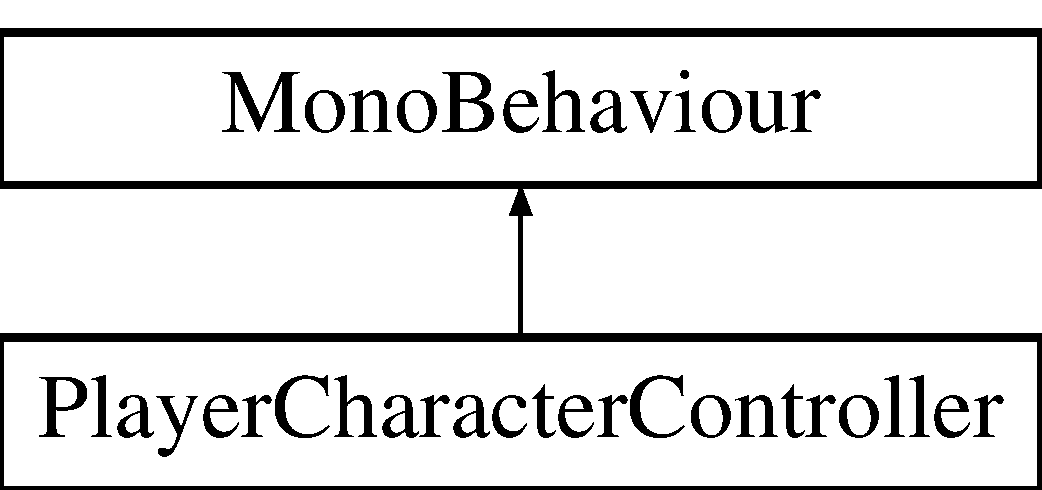
\includegraphics[height=2.000000cm]{class_player_character_controller}
\end{center}
\end{figure}
\subsection*{Public Member Functions}
\begin{DoxyCompactItemize}
\item 
\hypertarget{class_player_character_controller_afa2260da91d3f72d414e192353d89646}{void {\bfseries Move} (Vector3 start, Vector3 input, out Vector3 delta\-Move, out Vector3 position)}\label{class_player_character_controller_afa2260da91d3f72d414e192353d89646}

\end{DoxyCompactItemize}
\subsection*{Public Attributes}
\begin{DoxyCompactItemize}
\item 
\hypertarget{class_player_character_controller_aa7fa26a9c3b5494959cfd26ac3e55371}{Transform {\bfseries sprite\-Transform}}\label{class_player_character_controller_aa7fa26a9c3b5494959cfd26ac3e55371}

\item 
\hypertarget{class_player_character_controller_a55d2ff4f62604d521c28242e5ff9e8b2}{float {\bfseries speed}}\label{class_player_character_controller_a55d2ff4f62604d521c28242e5ff9e8b2}

\item 
\hypertarget{class_player_character_controller_aad00d245dd8416129b2c574792a8cc2c}{float {\bfseries sight}}\label{class_player_character_controller_aad00d245dd8416129b2c574792a8cc2c}

\item 
\hypertarget{class_player_character_controller_a11c68e7205de61cccbfdb516a5fa38e3}{Vector3 {\bfseries delta\-Move}}\label{class_player_character_controller_a11c68e7205de61cccbfdb516a5fa38e3}

\end{DoxyCompactItemize}


The documentation for this class was generated from the following file\-:\begin{DoxyCompactItemize}
\item 
/home/travis/build/temportalflux/\-Champ\-Net/\-Unity/\-Assets/\-Scripts/\-Player/Player\-Character\-Controller.\-cs\end{DoxyCompactItemize}

\hypertarget{class_player_input_controller}{\section{Player\-Input\-Controller Class Reference}
\label{class_player_input_controller}\index{Player\-Input\-Controller@{Player\-Input\-Controller}}
}
Inheritance diagram for Player\-Input\-Controller\-:\begin{figure}[H]
\begin{center}
\leavevmode
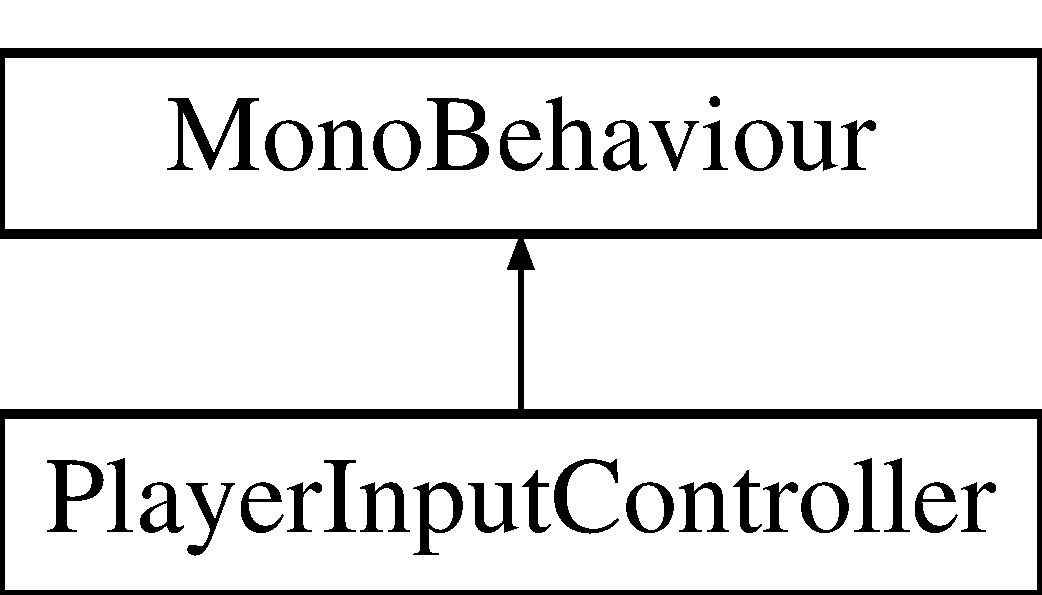
\includegraphics[height=2.000000cm]{class_player_input_controller}
\end{center}
\end{figure}
\subsection*{Public Member Functions}
\begin{DoxyCompactItemize}
\item 
\hypertarget{class_player_input_controller_aa617897cf92c385b734176b3c0f6a51b}{void {\bfseries Move} (Vector3 start, out Vector3 position, out Vector3 delta\-Move)}\label{class_player_input_controller_aa617897cf92c385b734176b3c0f6a51b}

\item 
\hypertarget{class_player_input_controller_a113e3417863a2d9ab228c795702607b3}{void {\bfseries on\-Axis} (Input\-Device device, Input\-Response.\-Update\-Event evt, Mapped\-Axis axis, Axis\-Direction value)}\label{class_player_input_controller_a113e3417863a2d9ab228c795702607b3}

\item 
\hypertarget{class_player_input_controller_a03be05ea0b3b1085b5633f59a9e131f5}{void {\bfseries on\-Axis} (Input\-Device device, Input\-Response.\-Update\-Event evt, Mapped\-Axis axis, float value)}\label{class_player_input_controller_a03be05ea0b3b1085b5633f59a9e131f5}

\item 
\hypertarget{class_player_input_controller_a9506d4adb70b38fb37a1f8171a53fa2e}{void {\bfseries on\-Axis\-Horizontal} (Input\-Device device, Input\-Response.\-Update\-Event evt, Mapped\-Axis axis, Axis\-Direction value)}\label{class_player_input_controller_a9506d4adb70b38fb37a1f8171a53fa2e}

\item 
\hypertarget{class_player_input_controller_a50f59443aa6b47628893eff83107c93e}{void {\bfseries on\-Axis\-Horizontal} (Input\-Device device, Input\-Response.\-Update\-Event evt, Mapped\-Axis axis, float value)}\label{class_player_input_controller_a50f59443aa6b47628893eff83107c93e}

\item 
\hypertarget{class_player_input_controller_abadac75139e4879a3de5d4e1947faa0e}{void {\bfseries on\-Axis\-Vertical} (Input\-Device device, Input\-Response.\-Update\-Event evt, Mapped\-Axis axis, Axis\-Direction value)}\label{class_player_input_controller_abadac75139e4879a3de5d4e1947faa0e}

\item 
\hypertarget{class_player_input_controller_ad97dbabee4ab8fccc583d38d2cd15447}{void {\bfseries on\-Axis\-Vertical} (Input\-Device device, Input\-Response.\-Update\-Event evt, Mapped\-Axis axis, float value)}\label{class_player_input_controller_ad97dbabee4ab8fccc583d38d2cd15447}

\end{DoxyCompactItemize}
\subsection*{Public Attributes}
\begin{DoxyCompactItemize}
\item 
\hypertarget{class_player_input_controller_ae7ad9ffda52758888cf9d6940d52e589}{Vector3 {\bfseries \-\_\-input}}\label{class_player_input_controller_ae7ad9ffda52758888cf9d6940d52e589}

\end{DoxyCompactItemize}


The documentation for this class was generated from the following file\-:\begin{DoxyCompactItemize}
\item 
/home/travis/build/temportalflux/\-Champ\-Net/\-Unity/\-Assets/\-Scripts/\-Player/Player\-Input\-Controller.\-cs\end{DoxyCompactItemize}

\hypertarget{class_player_local}{\section{Player\-Local Class Reference}
\label{class_player_local}\index{Player\-Local@{Player\-Local}}
}
Inheritance diagram for Player\-Local\-:\begin{figure}[H]
\begin{center}
\leavevmode
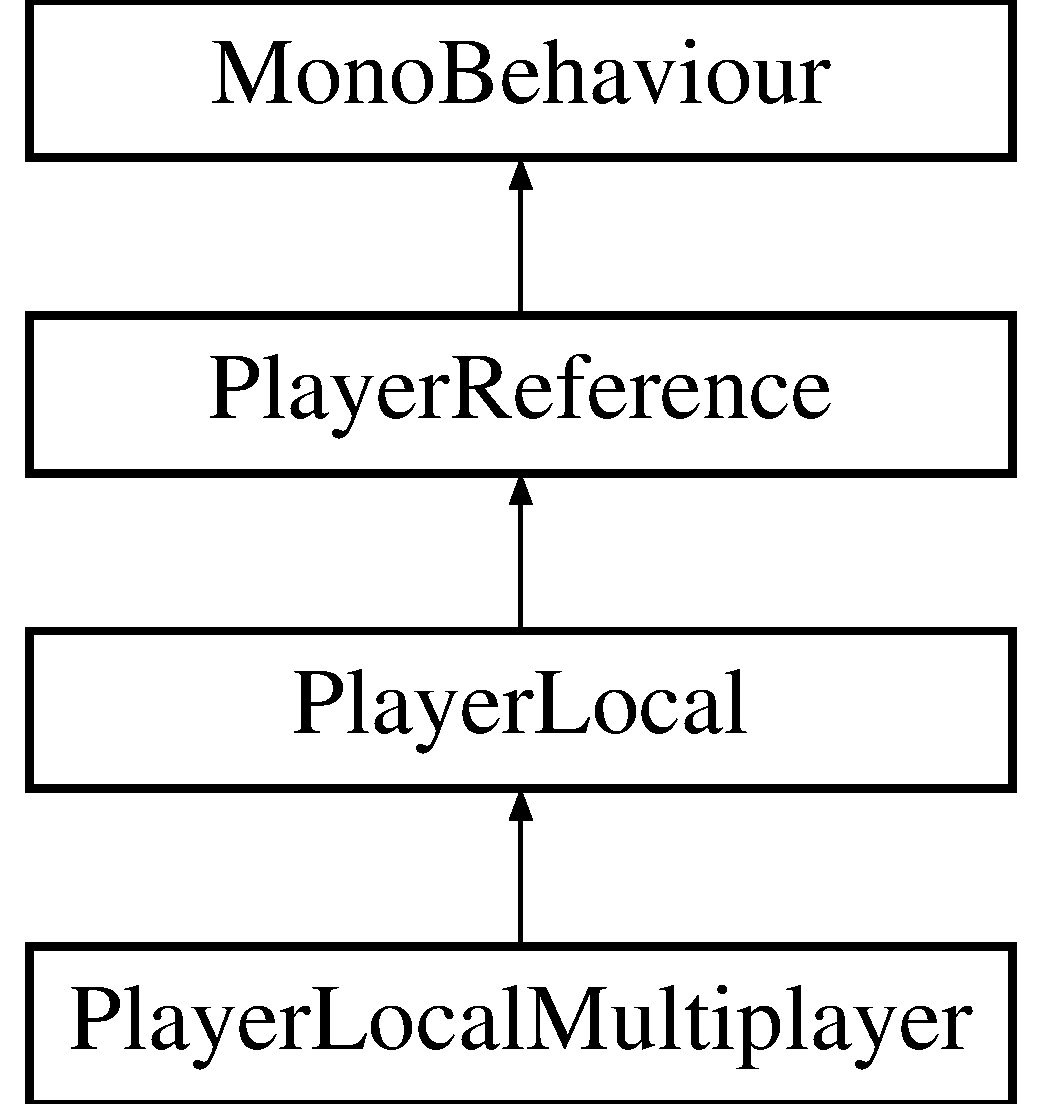
\includegraphics[height=4.000000cm]{class_player_local}
\end{center}
\end{figure}
\subsection*{Public Member Functions}
\begin{DoxyCompactItemize}
\item 
void \hyperlink{class_player_local_aa5c459588b976499120386eda1c1fac0}{challenge\-Random\-Player} ()
\begin{DoxyCompactList}\small\item\em Challenges the random player to a networked battle \end{DoxyCompactList}\item 
\hypertarget{class_player_local_aab51fb40e024127d177485ea82184dba}{void {\bfseries on\-Challenge\-By} (\hyperlink{class_monster_data_object}{Monster\-Data\-Object} opponent\-A\-I)}\label{class_player_local_aab51fb40e024127d177485ea82184dba}

\item 
void \hyperlink{class_player_local_a5344425e801a7f02419bf29ede2cb2af}{request\-Battle} (\hyperlink{class_player_reference}{Player\-Reference} player)
\begin{DoxyCompactList}\small\item\em Notifies the server of a battle request \end{DoxyCompactList}\item 
\hypertarget{class_player_local_a811782eb0815d88b3a1e5c8d23ee4903}{override void {\bfseries set\-Info} (\hyperlink{class_game_state_1_1_player}{Game\-State.\-Player} info)}\label{class_player_local_a811782eb0815d88b3a1e5c8d23ee4903}

\item 
\hypertarget{class_player_local_a71d5b41f860d3f8841f58a11aff1a6c3}{void {\bfseries request\-Move} ()}\label{class_player_local_a71d5b41f860d3f8841f58a11aff1a6c3}

\item 
void \hyperlink{class_player_local_ab718bcb062155f6de683dc8e78a799ba}{down} (Input\-Device device, Input\-Response.\-Update\-Event type, Mapped\-Button action)
\begin{DoxyCompactList}\small\item\em Only used to test scoreboard incrementation \end{DoxyCompactList}\end{DoxyCompactItemize}
\subsection*{Protected Member Functions}
\begin{DoxyCompactItemize}
\item 
\hypertarget{class_player_local_ab59f0a687fe4840df28008a6ea15eedf}{override void {\bfseries Awake} ()}\label{class_player_local_ab59f0a687fe4840df28008a6ea15eedf}

\item 
\hypertarget{class_player_local_ad2c22165846a385e21207c77e186b2c6}{override void {\bfseries Update} ()}\label{class_player_local_ad2c22165846a385e21207c77e186b2c6}

\end{DoxyCompactItemize}
\subsection*{Protected Attributes}
\begin{DoxyCompactItemize}
\item 
\hypertarget{class_player_local_ac8a46c71888c8feeabf3f6f8929fe34b}{\hyperlink{class_player_input_controller}{Player\-Input\-Controller} {\bfseries \-\_\-pic}}\label{class_player_local_ac8a46c71888c8feeabf3f6f8929fe34b}

\end{DoxyCompactItemize}
\subsection*{Additional Inherited Members}


\subsection{Member Function Documentation}
\hypertarget{class_player_local_aa5c459588b976499120386eda1c1fac0}{\index{Player\-Local@{Player\-Local}!challenge\-Random\-Player@{challenge\-Random\-Player}}
\index{challenge\-Random\-Player@{challenge\-Random\-Player}!PlayerLocal@{Player\-Local}}
\subsubsection[{challenge\-Random\-Player}]{\setlength{\rightskip}{0pt plus 5cm}void Player\-Local.\-challenge\-Random\-Player (
\begin{DoxyParamCaption}
{}
\end{DoxyParamCaption}
)\hspace{0.3cm}{\ttfamily [inline]}}}\label{class_player_local_aa5c459588b976499120386eda1c1fac0}


Challenges the random player to a networked battle 

Author\-: Dustin Yost \hypertarget{class_player_local_ab718bcb062155f6de683dc8e78a799ba}{\index{Player\-Local@{Player\-Local}!down@{down}}
\index{down@{down}!PlayerLocal@{Player\-Local}}
\subsubsection[{down}]{\setlength{\rightskip}{0pt plus 5cm}void Player\-Local.\-down (
\begin{DoxyParamCaption}
\item[{Input\-Device}]{device, }
\item[{Input\-Response.\-Update\-Event}]{type, }
\item[{Mapped\-Button}]{action}
\end{DoxyParamCaption}
)\hspace{0.3cm}{\ttfamily [inline]}}}\label{class_player_local_ab718bcb062155f6de683dc8e78a799ba}


Only used to test scoreboard incrementation 


\begin{DoxyParams}{Parameters}
{\em device} & \\
\hline
{\em type} & \\
\hline
{\em action} & \\
\hline
\end{DoxyParams}
$<$\-Author$>$ Christopher Brennan $<$/\-Author$>$ \hypertarget{class_player_local_a5344425e801a7f02419bf29ede2cb2af}{\index{Player\-Local@{Player\-Local}!request\-Battle@{request\-Battle}}
\index{request\-Battle@{request\-Battle}!PlayerLocal@{Player\-Local}}
\subsubsection[{request\-Battle}]{\setlength{\rightskip}{0pt plus 5cm}void Player\-Local.\-request\-Battle (
\begin{DoxyParamCaption}
\item[{{\bf Player\-Reference}}]{player}
\end{DoxyParamCaption}
)\hspace{0.3cm}{\ttfamily [inline]}}}\label{class_player_local_a5344425e801a7f02419bf29ede2cb2af}


Notifies the server of a battle request 


\begin{DoxyParams}{Parameters}
{\em player} & The player.\\
\hline
\end{DoxyParams}


Author\-: Dustin Yost 

The documentation for this class was generated from the following file\-:\begin{DoxyCompactItemize}
\item 
/home/travis/build/temportalflux/\-Champ\-Net/\-Unity/\-Assets/\-Scripts/\-Player/Player\-Local.\-cs\end{DoxyCompactItemize}

\hypertarget{class_player_local_multiplayer}{\section{Player\-Local\-Multiplayer Class Reference}
\label{class_player_local_multiplayer}\index{Player\-Local\-Multiplayer@{Player\-Local\-Multiplayer}}
}
Inheritance diagram for Player\-Local\-Multiplayer\-:\begin{figure}[H]
\begin{center}
\leavevmode
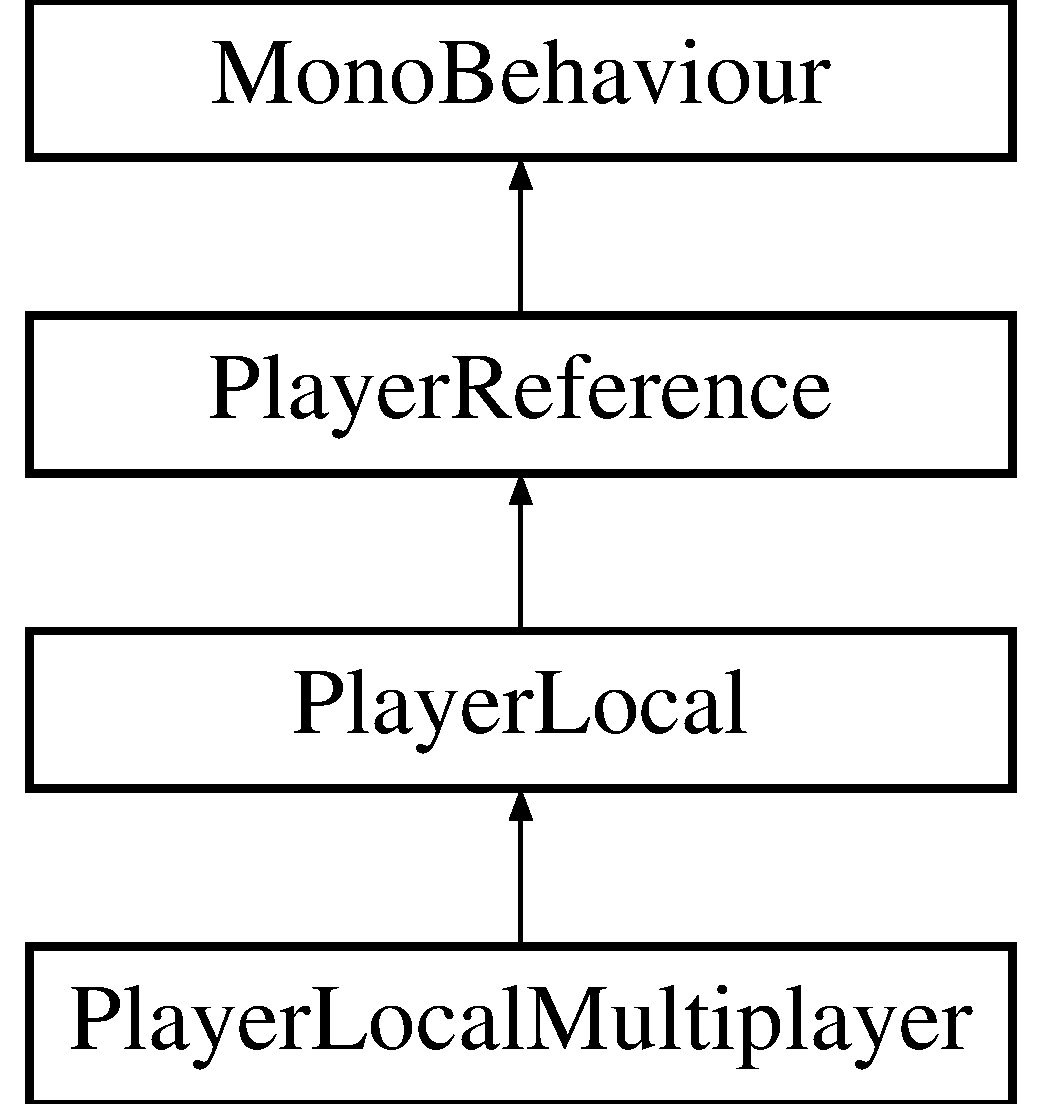
\includegraphics[height=4.000000cm]{class_player_local_multiplayer}
\end{center}
\end{figure}
\subsection*{Protected Member Functions}
\begin{DoxyCompactItemize}
\item 
\hypertarget{class_player_local_multiplayer_af8786075d98c26839e861fcf3cb3fbf8}{override void {\bfseries Update} ()}\label{class_player_local_multiplayer_af8786075d98c26839e861fcf3cb3fbf8}

\end{DoxyCompactItemize}
\subsection*{Additional Inherited Members}


The documentation for this class was generated from the following file\-:\begin{DoxyCompactItemize}
\item 
/home/travis/build/temportalflux/\-Champ\-Net/\-Unity/\-Assets/\-Scripts/\-Player/Player\-Local\-Multiplayer.\-cs\end{DoxyCompactItemize}

\hypertarget{class_player_network}{\section{Player\-Network Class Reference}
\label{class_player_network}\index{Player\-Network@{Player\-Network}}
}
Inheritance diagram for Player\-Network\-:\begin{figure}[H]
\begin{center}
\leavevmode
\includegraphics[height=3.000000cm]{class_player_network}
\end{center}
\end{figure}
\subsection*{Additional Inherited Members}


The documentation for this class was generated from the following file\-:\begin{DoxyCompactItemize}
\item 
/home/travis/build/temportalflux/\-Champ\-Net/\-Unity/\-Assets/\-Scripts/\-Player/Player\-Network.\-cs\end{DoxyCompactItemize}

\hypertarget{class_player_reference}{\section{Player\-Reference Class Reference}
\label{class_player_reference}\index{Player\-Reference@{Player\-Reference}}
}
Inheritance diagram for Player\-Reference\-:\begin{figure}[H]
\begin{center}
\leavevmode
\includegraphics[height=4.000000cm]{class_player_reference}
\end{center}
\end{figure}
\subsection*{Public Member Functions}
\begin{DoxyCompactItemize}
\item 
uint \hyperlink{class_player_reference_ae724ca461dddeed2f9671f9a745da381}{get\-I\-D} ()
\begin{DoxyCompactList}\small\item\em Gets the identifier. \end{DoxyCompactList}\item 
\hypertarget{class_player_reference_ae35eca907ad8238c4d51d65d8c021f26}{void {\bfseries set\-I\-D} (uint id)}\label{class_player_reference_ae35eca907ad8238c4d51d65d8c021f26}

\item 
void \hyperlink{class_player_reference_a4918fec4590780ff599dec4a5035bbbe}{integrate\-Info} (\hyperlink{struct_game_state_1_1_player}{Game\-State.\-Player} player\-Info, bool force\-Snap=false)
\begin{DoxyCompactList}\small\item\em Update the object to have some transform properties \end{DoxyCompactList}\item 
\hypertarget{class_player_reference_ab6b15f671b1553537a50db3529a74127}{\hyperlink{struct_game_state_1_1_player}{Game\-State.\-Player} {\bfseries get\-Info} ()}\label{class_player_reference_ab6b15f671b1553537a50db3529a74127}

\item 
\hypertarget{class_player_reference_aee764d4fed2e9c45ecdcfbf525bd03ed}{virtual void {\bfseries set\-Info} (\hyperlink{struct_game_state_1_1_player}{Game\-State.\-Player} info)}\label{class_player_reference_aee764d4fed2e9c45ecdcfbf525bd03ed}

\item 
\hypertarget{class_player_reference_aa8c16ecb182a8b2420158d87bdcdb510}{virtual void {\bfseries On\-Local\-Input} (Vector3 position, Vector3 delta\-Move)}\label{class_player_reference_aa8c16ecb182a8b2420158d87bdcdb510}

\end{DoxyCompactItemize}
\subsection*{Public Attributes}
\begin{DoxyCompactItemize}
\item 
\hypertarget{class_player_reference_a32979ccda155fe50f781e80c8bcfc5bd}{Transform {\bfseries sprite}}\label{class_player_reference_a32979ccda155fe50f781e80c8bcfc5bd}

\item 
\hypertarget{class_player_reference_a46a995f93fe98882b1a79d57b0baa66b}{Sprite\-Renderer {\bfseries overlay}}\label{class_player_reference_a46a995f93fe98882b1a79d57b0baa66b}

\item 
\hypertarget{class_player_reference_accd3ff8958657fee1e45aeb824b3e8e2}{Transform {\bfseries move\-Target}}\label{class_player_reference_accd3ff8958657fee1e45aeb824b3e8e2}

\end{DoxyCompactItemize}
\subsection*{Protected Member Functions}
\begin{DoxyCompactItemize}
\item 
\hypertarget{class_player_reference_adce9feacb370df0b0ea95754376aec04}{virtual void {\bfseries Awake} ()}\label{class_player_reference_adce9feacb370df0b0ea95754376aec04}

\item 
\hypertarget{class_player_reference_ad75981d8a0e56d56370a27b9fcca1e91}{virtual void {\bfseries Update} ()}\label{class_player_reference_ad75981d8a0e56d56370a27b9fcca1e91}

\end{DoxyCompactItemize}
\subsection*{Protected Attributes}
\begin{DoxyCompactItemize}
\item 
\hypertarget{class_player_reference_ae076e8379386c67d01beb3d76c3b4600}{\hyperlink{class_player_character_controller}{Player\-Character\-Controller} {\bfseries \-\_\-pcc}}\label{class_player_reference_ae076e8379386c67d01beb3d76c3b4600}

\item 
\hypertarget{class_player_reference_abffbcb7165e1d2fbb37b536d87eca369}{\hyperlink{struct_game_state_1_1_player}{Game\-State.\-Player} {\bfseries player\-Info}}\label{class_player_reference_abffbcb7165e1d2fbb37b536d87eca369}

\end{DoxyCompactItemize}
\subsection*{Properties}
\begin{DoxyCompactItemize}
\item 
uint \hyperlink{class_player_reference_ae0a1650c4dcd10b54eecdc1eca0edfb9}{score}\hspace{0.3cm}{\ttfamily  \mbox{[}get, set\mbox{]}}
\begin{DoxyCompactList}\small\item\em Score of the player \end{DoxyCompactList}\item 
uint \hyperlink{class_player_reference_ac06c2cae9b505a566de5d1b358ad9f51}{rank}\hspace{0.3cm}{\ttfamily  \mbox{[}get, set\mbox{]}}
\begin{DoxyCompactList}\small\item\em Current Rank of the player \end{DoxyCompactList}\end{DoxyCompactItemize}


\subsection{Member Function Documentation}
\hypertarget{class_player_reference_ae724ca461dddeed2f9671f9a745da381}{\index{Player\-Reference@{Player\-Reference}!get\-I\-D@{get\-I\-D}}
\index{get\-I\-D@{get\-I\-D}!PlayerReference@{Player\-Reference}}
\subsubsection[{get\-I\-D}]{\setlength{\rightskip}{0pt plus 5cm}uint Player\-Reference.\-get\-I\-D (
\begin{DoxyParamCaption}
{}
\end{DoxyParamCaption}
)\hspace{0.3cm}{\ttfamily [inline]}}}\label{class_player_reference_ae724ca461dddeed2f9671f9a745da381}


Gets the identifier. 

\begin{DoxyReturn}{Returns}

\end{DoxyReturn}
\hypertarget{class_player_reference_a4918fec4590780ff599dec4a5035bbbe}{\index{Player\-Reference@{Player\-Reference}!integrate\-Info@{integrate\-Info}}
\index{integrate\-Info@{integrate\-Info}!PlayerReference@{Player\-Reference}}
\subsubsection[{integrate\-Info}]{\setlength{\rightskip}{0pt plus 5cm}void Player\-Reference.\-integrate\-Info (
\begin{DoxyParamCaption}
\item[{{\bf Game\-State.\-Player}}]{player\-Info, }
\item[{bool}]{force\-Snap = {\ttfamily false}}
\end{DoxyParamCaption}
)\hspace{0.3cm}{\ttfamily [inline]}}}\label{class_player_reference_a4918fec4590780ff599dec4a5035bbbe}


Update the object to have some transform properties 


\begin{DoxyParams}{Parameters}
{\em pos\-X} & The position x.\\
\hline
{\em pos\-Y} & The position y.\\
\hline
{\em vel\-X} & The rot z.\\
\hline
{\em vel\-Y} & \\
\hline
\end{DoxyParams}


Author\-: Dustin Yost 

\subsection{Property Documentation}
\hypertarget{class_player_reference_ac06c2cae9b505a566de5d1b358ad9f51}{\index{Player\-Reference@{Player\-Reference}!rank@{rank}}
\index{rank@{rank}!PlayerReference@{Player\-Reference}}
\subsubsection[{rank}]{\setlength{\rightskip}{0pt plus 5cm}uint Player\-Reference.\-rank\hspace{0.3cm}{\ttfamily [get]}, {\ttfamily [set]}}}\label{class_player_reference_ac06c2cae9b505a566de5d1b358ad9f51}


Current Rank of the player 

\hypertarget{class_player_reference_ae0a1650c4dcd10b54eecdc1eca0edfb9}{\index{Player\-Reference@{Player\-Reference}!score@{score}}
\index{score@{score}!PlayerReference@{Player\-Reference}}
\subsubsection[{score}]{\setlength{\rightskip}{0pt plus 5cm}uint Player\-Reference.\-score\hspace{0.3cm}{\ttfamily [get]}, {\ttfamily [set]}}}\label{class_player_reference_ae0a1650c4dcd10b54eecdc1eca0edfb9}


Score of the player 



The documentation for this class was generated from the following file\-:\begin{DoxyCompactItemize}
\item 
/home/travis/build/temportalflux/\-Champ\-Net/\-Unity/\-Assets/\-Scripts/\-Player/Player\-Reference.\-cs\end{DoxyCompactItemize}

\hypertarget{class_score_board_1_1_rank_text}{\section{Score\-Board.\-Rank\-Text Class Reference}
\label{class_score_board_1_1_rank_text}\index{Score\-Board.\-Rank\-Text@{Score\-Board.\-Rank\-Text}}
}
\subsection*{Public Attributes}
\begin{DoxyCompactItemize}
\item 
\hypertarget{class_score_board_1_1_rank_text_ad1bb11aeb2005a31c4202c82958dd899}{int {\bfseries Rank}}\label{class_score_board_1_1_rank_text_ad1bb11aeb2005a31c4202c82958dd899}

\item 
\hypertarget{class_score_board_1_1_rank_text_a7cd14f47e2a22acedbecf27fd100f8fd}{int {\bfseries font\-Size}}\label{class_score_board_1_1_rank_text_a7cd14f47e2a22acedbecf27fd100f8fd}

\item 
\hypertarget{class_score_board_1_1_rank_text_a7fe435f4d04ade5af1b00d67a523cfdf}{Font\-Style {\bfseries font\-Style}}\label{class_score_board_1_1_rank_text_a7fe435f4d04ade5af1b00d67a523cfdf}

\item 
\hypertarget{class_score_board_1_1_rank_text_adbf90323214eddb0b4d7fc5287ad7549}{Font {\bfseries font}}\label{class_score_board_1_1_rank_text_adbf90323214eddb0b4d7fc5287ad7549}

\item 
\hypertarget{class_score_board_1_1_rank_text_ae8f670f701a8007114c80981c4bf3ce7}{Game\-Object {\bfseries Name\-Object}}\label{class_score_board_1_1_rank_text_ae8f670f701a8007114c80981c4bf3ce7}

\item 
\hypertarget{class_score_board_1_1_rank_text_a558c65dcc4b67d850be54e47dc91fff0}{Game\-Object {\bfseries Win\-Object}}\label{class_score_board_1_1_rank_text_a558c65dcc4b67d850be54e47dc91fff0}

\item 
\hypertarget{class_score_board_1_1_rank_text_a6f7701cb446d574c4a5ea7cec611ba2b}{string {\bfseries name}}\label{class_score_board_1_1_rank_text_a6f7701cb446d574c4a5ea7cec611ba2b}

\item 
\hypertarget{class_score_board_1_1_rank_text_a13ad6b821540d3fce3650a4590dabfc5}{uint {\bfseries score}}\label{class_score_board_1_1_rank_text_a13ad6b821540d3fce3650a4590dabfc5}

\item 
\hypertarget{class_score_board_1_1_rank_text_a370ca923374efc2137c9d54c38f7901e}{int {\bfseries I\-D}}\label{class_score_board_1_1_rank_text_a370ca923374efc2137c9d54c38f7901e}

\end{DoxyCompactItemize}


The documentation for this class was generated from the following file\-:\begin{DoxyCompactItemize}
\item 
/home/travis/build/temportalflux/\-Champ\-Net/\-Unity/\-Assets/\-Scripts/\-U\-I/Score\-Board.\-cs\end{DoxyCompactItemize}

\hypertarget{class_scene_transition}{\section{Scene\-Transition Class Reference}
\label{class_scene_transition}\index{Scene\-Transition@{Scene\-Transition}}
}
Inheritance diagram for Scene\-Transition\-:\begin{figure}[H]
\begin{center}
\leavevmode
\includegraphics[height=2.000000cm]{class_scene_transition}
\end{center}
\end{figure}
\subsection*{Public Member Functions}
\begin{DoxyCompactItemize}
\item 
\hypertarget{class_scene_transition_ac0f7927206a866304c59c6f9d64db781}{void {\bfseries load} (Manager\-Transitions.\-On\-Transition\-Finish on\-Finish=null)}\label{class_scene_transition_ac0f7927206a866304c59c6f9d64db781}

\item 
\hypertarget{class_scene_transition_a1c56080a413a75527ecc5aaea65d5897}{void {\bfseries exit} (Manager\-Transitions.\-On\-Transition\-Finish on\-Finish=null)}\label{class_scene_transition_a1c56080a413a75527ecc5aaea65d5897}

\end{DoxyCompactItemize}
\subsection*{Public Attributes}
\begin{DoxyCompactItemize}
\item 
\hypertarget{class_scene_transition_a38658b7f48d29d07b9d79a9b77bbb4ee}{string {\bfseries next\-Scene}}\label{class_scene_transition_a38658b7f48d29d07b9d79a9b77bbb4ee}

\item 
\hypertarget{class_scene_transition_a5b140f4b742c3d71eaaedbee3a52a588}{Load\-Scene\-Mode {\bfseries load\-Mode}}\label{class_scene_transition_a5b140f4b742c3d71eaaedbee3a52a588}

\end{DoxyCompactItemize}


The documentation for this class was generated from the following file\-:\begin{DoxyCompactItemize}
\item 
/home/travis/build/temportalflux/\-Champ\-Net/\-Unity/\-Assets/\-Scripts/\-Transitions/Scene\-Transition.\-cs\end{DoxyCompactItemize}

\hypertarget{class_score_board}{\section{Score\-Board Class Reference}
\label{class_score_board}\index{Score\-Board@{Score\-Board}}
}
Inheritance diagram for Score\-Board\-:\begin{figure}[H]
\begin{center}
\leavevmode
\includegraphics[height=2.000000cm]{class_score_board}
\end{center}
\end{figure}
\subsection*{Classes}
\begin{DoxyCompactItemize}
\item 
class \hyperlink{class_score_board_1_1_rank_text}{Rank\-Text}
\end{DoxyCompactItemize}
\subsection*{Public Member Functions}
\begin{DoxyCompactItemize}
\item 
void \hyperlink{class_score_board_a67bd4682926000724ae01e01c3e79f66}{Display\-Score\-Board} ()
\begin{DoxyCompactList}\small\item\em updates scoreboard on player win \end{DoxyCompactList}\item 
\hypertarget{class_score_board_a5ece9a1f2b00f8f91715f62ff50e7143}{void {\bfseries remove\-Player\-On\-Leave} (uint remove\-Name)}\label{class_score_board_a5ece9a1f2b00f8f91715f62ff50e7143}

\end{DoxyCompactItemize}
\subsection*{Public Attributes}
\begin{DoxyCompactItemize}
\item 
\hypertarget{class_score_board_ac363bd13d0776f76c58860a4df02d52a}{Game\-Object {\bfseries Name\-Header}}\label{class_score_board_ac363bd13d0776f76c58860a4df02d52a}

\item 
\hypertarget{class_score_board_a305d151ef51ca2eff7dc1d59e7b36927}{Game\-Object {\bfseries Win\-Header}}\label{class_score_board_a305d151ef51ca2eff7dc1d59e7b36927}

\item 
\hypertarget{class_score_board_aed96e15fc6ad9463d3257b677b3ef6ed}{Camera {\bfseries the\-Camera}}\label{class_score_board_aed96e15fc6ad9463d3257b677b3ef6ed}

\item 
\hypertarget{class_score_board_ac2dbac3428216b7faaa8d344efda9b73}{\hyperlink{class_score_board_1_1_rank_text}{Rank\-Text}\mbox{[}$\,$\mbox{]} {\bfseries rank\-Text}}\label{class_score_board_ac2dbac3428216b7faaa8d344efda9b73}

\end{DoxyCompactItemize}


\subsection{Member Function Documentation}
\hypertarget{class_score_board_a67bd4682926000724ae01e01c3e79f66}{\index{Score\-Board@{Score\-Board}!Display\-Score\-Board@{Display\-Score\-Board}}
\index{Display\-Score\-Board@{Display\-Score\-Board}!ScoreBoard@{Score\-Board}}
\subsubsection[{Display\-Score\-Board}]{\setlength{\rightskip}{0pt plus 5cm}void Score\-Board.\-Display\-Score\-Board (
\begin{DoxyParamCaption}
{}
\end{DoxyParamCaption}
)\hspace{0.3cm}{\ttfamily [inline]}}}\label{class_score_board_a67bd4682926000724ae01e01c3e79f66}


updates scoreboard on player win 

left to do\-: remove player from board when they leave // call function on player disconnect notification 

Author\-: Christopher Brennan 

The documentation for this class was generated from the following file\-:\begin{DoxyCompactItemize}
\item 
/home/travis/build/temportalflux/\-Champ\-Net/\-Unity/\-Assets/\-Scripts/\-U\-I/Score\-Board.\-cs\end{DoxyCompactItemize}

\hypertarget{class_scoreboard_increment_test}{\section{Scoreboard\-Increment\-Test Class Reference}
\label{class_scoreboard_increment_test}\index{Scoreboard\-Increment\-Test@{Scoreboard\-Increment\-Test}}
}
Inheritance diagram for Scoreboard\-Increment\-Test\-:\begin{figure}[H]
\begin{center}
\leavevmode
\includegraphics[height=2.000000cm]{class_scoreboard_increment_test}
\end{center}
\end{figure}
\subsection*{Public Member Functions}
\begin{DoxyCompactItemize}
\item 
\hypertarget{class_scoreboard_increment_test_a727b58ab4929807cb1b363aef6cb630c}{void {\bfseries down} (Input\-Device device, Input\-Response.\-Update\-Event type, Mapped\-Button action)}\label{class_scoreboard_increment_test_a727b58ab4929807cb1b363aef6cb630c}

\end{DoxyCompactItemize}


The documentation for this class was generated from the following file\-:\begin{DoxyCompactItemize}
\item 
/home/travis/build/temportalflux/\-Champ\-Net/\-Unity/\-Assets/\-Scripts/\-U\-I/Scoreboard\-Increment\-Test.\-cs\end{DoxyCompactItemize}

\hypertarget{class_bit_test_1_1_sereal}{\section{Bit\-Test.\-Sereal Class Reference}
\label{class_bit_test_1_1_sereal}\index{Bit\-Test.\-Sereal@{Bit\-Test.\-Sereal}}
}
Inheritance diagram for Bit\-Test.\-Sereal\-:\begin{figure}[H]
\begin{center}
\leavevmode
\includegraphics[height=2.000000cm]{class_bit_test_1_1_sereal}
\end{center}
\end{figure}
\subsection*{Public Member Functions}
\begin{DoxyCompactItemize}
\item 
int \hyperlink{class_bit_test_1_1_sereal_aba8f9fa60b53f974ddd59bf83f56fd35}{Get\-Size} ()
\begin{DoxyCompactList}\small\item\em Returns the size of the packet (the size for a potential byte\mbox{[}\mbox{]}) \end{DoxyCompactList}\item 
void \hyperlink{class_bit_test_1_1_sereal_ad5a8343dbe518ffa4c1b99db449638ad}{Serialize} (ref byte\mbox{[}$\,$\mbox{]} data, ref int last\-Index)
\begin{DoxyCompactList}\small\item\em Serializes data from this event into a byte array \end{DoxyCompactList}\item 
void \hyperlink{class_bit_test_1_1_sereal_a09fd14bfb4c58714302d127a3e5030d7}{Deserialize} (byte\mbox{[}$\,$\mbox{]} data, ref int last\-Index)
\begin{DoxyCompactList}\small\item\em Deserializes data from a byte array into this event's data \end{DoxyCompactList}\end{DoxyCompactItemize}
\subsection*{Public Attributes}
\begin{DoxyCompactItemize}
\item 
\hypertarget{class_bit_test_1_1_sereal_a3139b4f271309ee788f73f102d3c1661}{uint {\bfseries client\-I\-D}}\label{class_bit_test_1_1_sereal_a3139b4f271309ee788f73f102d3c1661}

\item 
\hypertarget{class_bit_test_1_1_sereal_a986b0c99c646bb6239c1980c31eba9ca}{Color {\bfseries color}}\label{class_bit_test_1_1_sereal_a986b0c99c646bb6239c1980c31eba9ca}

\end{DoxyCompactItemize}


\subsection{Member Function Documentation}
\hypertarget{class_bit_test_1_1_sereal_a09fd14bfb4c58714302d127a3e5030d7}{\index{Bit\-Test\-::\-Sereal@{Bit\-Test\-::\-Sereal}!Deserialize@{Deserialize}}
\index{Deserialize@{Deserialize}!BitTest::Sereal@{Bit\-Test\-::\-Sereal}}
\subsubsection[{Deserialize}]{\setlength{\rightskip}{0pt plus 5cm}void Bit\-Test.\-Sereal.\-Deserialize (
\begin{DoxyParamCaption}
\item[{byte\mbox{[}$\,$\mbox{]}}]{data, }
\item[{ref int}]{last\-Index}
\end{DoxyParamCaption}
)\hspace{0.3cm}{\ttfamily [inline]}}}\label{class_bit_test_1_1_sereal_a09fd14bfb4c58714302d127a3e5030d7}


Deserializes data from a byte array into this event's data 


\begin{DoxyParams}{Parameters}
{\em data} & The data.\\
\hline
{\em last\-Index} & The last index.\\
\hline
\end{DoxyParams}


Author\-: Dustin Yost 

Implements \hyperlink{interface_i_serializing_a92f8ba3a06d21e7b01e37411e4e3145c}{I\-Serializing}.

\hypertarget{class_bit_test_1_1_sereal_aba8f9fa60b53f974ddd59bf83f56fd35}{\index{Bit\-Test\-::\-Sereal@{Bit\-Test\-::\-Sereal}!Get\-Size@{Get\-Size}}
\index{Get\-Size@{Get\-Size}!BitTest::Sereal@{Bit\-Test\-::\-Sereal}}
\subsubsection[{Get\-Size}]{\setlength{\rightskip}{0pt plus 5cm}int Bit\-Test.\-Sereal.\-Get\-Size (
\begin{DoxyParamCaption}
{}
\end{DoxyParamCaption}
)\hspace{0.3cm}{\ttfamily [inline]}}}\label{class_bit_test_1_1_sereal_aba8f9fa60b53f974ddd59bf83f56fd35}


Returns the size of the packet (the size for a potential byte\mbox{[}\mbox{]}) 

\begin{DoxyReturn}{Returns}
the integer length of a byte array to hold this event's data 
\end{DoxyReturn}


Author\-: Dustin Yost 

Implements \hyperlink{interface_i_serializing_a9e6ea0afaeac8d1d57e20579f87bebe2}{I\-Serializing}.

\hypertarget{class_bit_test_1_1_sereal_ad5a8343dbe518ffa4c1b99db449638ad}{\index{Bit\-Test\-::\-Sereal@{Bit\-Test\-::\-Sereal}!Serialize@{Serialize}}
\index{Serialize@{Serialize}!BitTest::Sereal@{Bit\-Test\-::\-Sereal}}
\subsubsection[{Serialize}]{\setlength{\rightskip}{0pt plus 5cm}void Bit\-Test.\-Sereal.\-Serialize (
\begin{DoxyParamCaption}
\item[{ref byte\mbox{[}$\,$\mbox{]}}]{data, }
\item[{ref int}]{last\-Index}
\end{DoxyParamCaption}
)\hspace{0.3cm}{\ttfamily [inline]}}}\label{class_bit_test_1_1_sereal_ad5a8343dbe518ffa4c1b99db449638ad}


Serializes data from this event into a byte array 


\begin{DoxyParams}{Parameters}
{\em data} & The data.\\
\hline
{\em last\-Index} & The last index.\\
\hline
\end{DoxyParams}


Author\-: Dustin Yost 

Implements \hyperlink{interface_i_serializing_ac31a44c2358a197e774fa3f79cc80356}{I\-Serializing}.



The documentation for this class was generated from the following file\-:\begin{DoxyCompactItemize}
\item 
/home/travis/build/temportalflux/\-Champ\-Net/\-Unity/\-Assets/\-Scripts/\-Attribute/Bit\-Test.\-cs\end{DoxyCompactItemize}

\hypertarget{class_bit_serialize_attribute_1_1_serialization_module_3_01_t_01_4}{\section{Bit\-Serialize\-Attribute.\-Serialization\-Module$<$ T $>$ Class Template Reference}
\label{class_bit_serialize_attribute_1_1_serialization_module_3_01_t_01_4}\index{Bit\-Serialize\-Attribute.\-Serialization\-Module$<$ T $>$@{Bit\-Serialize\-Attribute.\-Serialization\-Module$<$ T $>$}}
}


The implementation of \hyperlink{interface_bit_serialize_attribute_1_1_i_serialization_module}{I\-Serialization\-Module}, where all the generic \char`\"{}object\char`\"{} fields are objects with the type T.  


Inheritance diagram for Bit\-Serialize\-Attribute.\-Serialization\-Module$<$ T $>$\-:\begin{figure}[H]
\begin{center}
\leavevmode
\includegraphics[height=2.000000cm]{class_bit_serialize_attribute_1_1_serialization_module_3_01_t_01_4}
\end{center}
\end{figure}
\subsection*{Public Member Functions}
\begin{DoxyCompactItemize}
\item 
int \hyperlink{class_bit_serialize_attribute_1_1_serialization_module_3_01_t_01_4_a2ab6b7e0f1e8eccfe929221a4c86c0b3}{Get\-Size} (object obj)
\begin{DoxyCompactList}\small\item\em Determine the size of some object -\/ effectively sizeof(object). \end{DoxyCompactList}\item 
byte\mbox{[}$\,$\mbox{]} \hyperlink{class_bit_serialize_attribute_1_1_serialization_module_3_01_t_01_4_a566f48c068bafbe25a9d3371afb83892}{Serialize} (object obj, byte\mbox{[}$\,$\mbox{]} data, int start)
\begin{DoxyCompactList}\small\item\em Serialize a specfic object into a byte array. Returns the byte\mbox{[}\mbox{]} with the populated data. \end{DoxyCompactList}\item 
object \hyperlink{class_bit_serialize_attribute_1_1_serialization_module_3_01_t_01_4_a7259a654093fa61bab6ef3766d13a12e}{Deserialize} (object obj, byte\mbox{[}$\,$\mbox{]} data, int start, Type type)
\begin{DoxyCompactList}\small\item\em Deserialize a byte array into an object with the type T. \end{DoxyCompactList}\end{DoxyCompactItemize}
\subsection*{Public Attributes}
\begin{DoxyCompactItemize}
\item 
Func$<$ T, int $>$ \hyperlink{class_bit_serialize_attribute_1_1_serialization_module_3_01_t_01_4_ae7b34baf697be55e822689dddd3d8dca}{\-\_\-\-Get\-Size}
\begin{DoxyCompactList}\small\item\em A generic, and module settable, version of \hyperlink{interface_bit_serialize_attribute_1_1_i_serialization_module_a057ba8b3168eb8a0999a329cca222cea}{I\-Serialization\-Module.\-Get\-Size(object)}. \end{DoxyCompactList}\item 
Func$<$ T, byte\mbox{[}$\,$\mbox{]}, int, byte\mbox{[}$\,$\mbox{]}$>$ \hyperlink{class_bit_serialize_attribute_1_1_serialization_module_3_01_t_01_4_a2e3a228e7b2cfe75c555a69c859f6564}{\-\_\-\-Serialize}
\begin{DoxyCompactList}\small\item\em A generic, and module settable, version of \hyperlink{interface_bit_serialize_attribute_1_1_i_serialization_module_ad3b3d5f329538f550958a8342d9e0708}{I\-Serialization\-Module.\-Serialize(object, byte\mbox{[}$\,$\mbox{]}, int)}. \end{DoxyCompactList}\item 
Func$<$ T, byte\mbox{[}$\,$\mbox{]}, int, Type, T $>$ \hyperlink{class_bit_serialize_attribute_1_1_serialization_module_3_01_t_01_4_a888f4fda944e93208eddd2368b2ed5a2}{\-\_\-\-Deserialize}
\begin{DoxyCompactList}\small\item\em A generic, and module settable, version of I\-Serialization\-Module.\-Deserialize(byte\mbox{[}$\,$\mbox{]}, int). \end{DoxyCompactList}\end{DoxyCompactItemize}


\subsection{Detailed Description}
The implementation of \hyperlink{interface_bit_serialize_attribute_1_1_i_serialization_module}{I\-Serialization\-Module}, where all the generic \char`\"{}object\char`\"{} fields are objects with the type T. 


\begin{DoxyTemplParams}{Template Parameters}
{\em T} & The generic type which this struct wraps the (De)Serialization of.\\
\hline
\end{DoxyTemplParams}


\subsection{Member Function Documentation}
\hypertarget{class_bit_serialize_attribute_1_1_serialization_module_3_01_t_01_4_a7259a654093fa61bab6ef3766d13a12e}{\index{Bit\-Serialize\-Attribute\-::\-Serialization\-Module$<$ T $>$@{Bit\-Serialize\-Attribute\-::\-Serialization\-Module$<$ T $>$}!Deserialize@{Deserialize}}
\index{Deserialize@{Deserialize}!BitSerializeAttribute::SerializationModule< T >@{Bit\-Serialize\-Attribute\-::\-Serialization\-Module$<$ T $>$}}
\subsubsection[{Deserialize}]{\setlength{\rightskip}{0pt plus 5cm}object Bit\-Serialize\-Attribute.\-Serialization\-Module$<$ T $>$.Deserialize (
\begin{DoxyParamCaption}
\item[{object}]{obj, }
\item[{byte\mbox{[}$\,$\mbox{]}}]{data, }
\item[{int}]{start, }
\item[{Type}]{type}
\end{DoxyParamCaption}
)\hspace{0.3cm}{\ttfamily [inline]}}}\label{class_bit_serialize_attribute_1_1_serialization_module_3_01_t_01_4_a7259a654093fa61bab6ef3766d13a12e}


Deserialize a byte array into an object with the type T. 


\begin{DoxyParams}{Parameters}
{\em data} & the byte\mbox{[}\mbox{]} of data.\\
\hline
{\em start} & How far into the serialized data the object was put.\\
\hline
\end{DoxyParams}
\begin{DoxyReturn}{Returns}
object with the type T
\end{DoxyReturn}


Implements \hyperlink{interface_bit_serialize_attribute_1_1_i_serialization_module_a9c1c3c1a875354c8d3320e99c63da4a4}{Bit\-Serialize\-Attribute.\-I\-Serialization\-Module}.

\hypertarget{class_bit_serialize_attribute_1_1_serialization_module_3_01_t_01_4_a2ab6b7e0f1e8eccfe929221a4c86c0b3}{\index{Bit\-Serialize\-Attribute\-::\-Serialization\-Module$<$ T $>$@{Bit\-Serialize\-Attribute\-::\-Serialization\-Module$<$ T $>$}!Get\-Size@{Get\-Size}}
\index{Get\-Size@{Get\-Size}!BitSerializeAttribute::SerializationModule< T >@{Bit\-Serialize\-Attribute\-::\-Serialization\-Module$<$ T $>$}}
\subsubsection[{Get\-Size}]{\setlength{\rightskip}{0pt plus 5cm}int Bit\-Serialize\-Attribute.\-Serialization\-Module$<$ T $>$.Get\-Size (
\begin{DoxyParamCaption}
\item[{object}]{obj}
\end{DoxyParamCaption}
)\hspace{0.3cm}{\ttfamily [inline]}}}\label{class_bit_serialize_attribute_1_1_serialization_module_3_01_t_01_4_a2ab6b7e0f1e8eccfe929221a4c86c0b3}


Determine the size of some object -\/ effectively sizeof(object). 


\begin{DoxyParams}{Parameters}
{\em obj} & The object with the type T.\\
\hline
\end{DoxyParams}
\begin{DoxyReturn}{Returns}
int
\end{DoxyReturn}


Implements \hyperlink{interface_bit_serialize_attribute_1_1_i_serialization_module_a057ba8b3168eb8a0999a329cca222cea}{Bit\-Serialize\-Attribute.\-I\-Serialization\-Module}.

\hypertarget{class_bit_serialize_attribute_1_1_serialization_module_3_01_t_01_4_a566f48c068bafbe25a9d3371afb83892}{\index{Bit\-Serialize\-Attribute\-::\-Serialization\-Module$<$ T $>$@{Bit\-Serialize\-Attribute\-::\-Serialization\-Module$<$ T $>$}!Serialize@{Serialize}}
\index{Serialize@{Serialize}!BitSerializeAttribute::SerializationModule< T >@{Bit\-Serialize\-Attribute\-::\-Serialization\-Module$<$ T $>$}}
\subsubsection[{Serialize}]{\setlength{\rightskip}{0pt plus 5cm}byte \mbox{[}$\,$\mbox{]} Bit\-Serialize\-Attribute.\-Serialization\-Module$<$ T $>$.Serialize (
\begin{DoxyParamCaption}
\item[{object}]{obj, }
\item[{byte\mbox{[}$\,$\mbox{]}}]{data, }
\item[{int}]{start}
\end{DoxyParamCaption}
)\hspace{0.3cm}{\ttfamily [inline]}}}\label{class_bit_serialize_attribute_1_1_serialization_module_3_01_t_01_4_a566f48c068bafbe25a9d3371afb83892}


Serialize a specfic object into a byte array. Returns the byte\mbox{[}\mbox{]} with the populated data. 


\begin{DoxyParams}{Parameters}
{\em obj} & The object to serialize with the type T.\\
\hline
{\em data} & The byte array of data.\\
\hline
{\em start} & How far into the data to put the object's serialized data.\\
\hline
\end{DoxyParams}
\begin{DoxyReturn}{Returns}
byte\mbox{[}\mbox{]}
\end{DoxyReturn}


Implements \hyperlink{interface_bit_serialize_attribute_1_1_i_serialization_module_ad3b3d5f329538f550958a8342d9e0708}{Bit\-Serialize\-Attribute.\-I\-Serialization\-Module}.



\subsection{Member Data Documentation}
\hypertarget{class_bit_serialize_attribute_1_1_serialization_module_3_01_t_01_4_a888f4fda944e93208eddd2368b2ed5a2}{\index{Bit\-Serialize\-Attribute\-::\-Serialization\-Module$<$ T $>$@{Bit\-Serialize\-Attribute\-::\-Serialization\-Module$<$ T $>$}!\-\_\-\-Deserialize@{\-\_\-\-Deserialize}}
\index{\-\_\-\-Deserialize@{\-\_\-\-Deserialize}!BitSerializeAttribute::SerializationModule< T >@{Bit\-Serialize\-Attribute\-::\-Serialization\-Module$<$ T $>$}}
\subsubsection[{\-\_\-\-Deserialize}]{\setlength{\rightskip}{0pt plus 5cm}Func$<$T, byte\mbox{[}$\,$\mbox{]}, int, Type, T$>$ Bit\-Serialize\-Attribute.\-Serialization\-Module$<$ T $>$.\-\_\-\-Deserialize}}\label{class_bit_serialize_attribute_1_1_serialization_module_3_01_t_01_4_a888f4fda944e93208eddd2368b2ed5a2}


A generic, and module settable, version of I\-Serialization\-Module.\-Deserialize(byte\mbox{[}$\,$\mbox{]}, int). 

\hypertarget{class_bit_serialize_attribute_1_1_serialization_module_3_01_t_01_4_ae7b34baf697be55e822689dddd3d8dca}{\index{Bit\-Serialize\-Attribute\-::\-Serialization\-Module$<$ T $>$@{Bit\-Serialize\-Attribute\-::\-Serialization\-Module$<$ T $>$}!\-\_\-\-Get\-Size@{\-\_\-\-Get\-Size}}
\index{\-\_\-\-Get\-Size@{\-\_\-\-Get\-Size}!BitSerializeAttribute::SerializationModule< T >@{Bit\-Serialize\-Attribute\-::\-Serialization\-Module$<$ T $>$}}
\subsubsection[{\-\_\-\-Get\-Size}]{\setlength{\rightskip}{0pt plus 5cm}Func$<$T, int$>$ Bit\-Serialize\-Attribute.\-Serialization\-Module$<$ T $>$.\-\_\-\-Get\-Size}}\label{class_bit_serialize_attribute_1_1_serialization_module_3_01_t_01_4_ae7b34baf697be55e822689dddd3d8dca}


A generic, and module settable, version of \hyperlink{interface_bit_serialize_attribute_1_1_i_serialization_module_a057ba8b3168eb8a0999a329cca222cea}{I\-Serialization\-Module.\-Get\-Size(object)}. 

\hypertarget{class_bit_serialize_attribute_1_1_serialization_module_3_01_t_01_4_a2e3a228e7b2cfe75c555a69c859f6564}{\index{Bit\-Serialize\-Attribute\-::\-Serialization\-Module$<$ T $>$@{Bit\-Serialize\-Attribute\-::\-Serialization\-Module$<$ T $>$}!\-\_\-\-Serialize@{\-\_\-\-Serialize}}
\index{\-\_\-\-Serialize@{\-\_\-\-Serialize}!BitSerializeAttribute::SerializationModule< T >@{Bit\-Serialize\-Attribute\-::\-Serialization\-Module$<$ T $>$}}
\subsubsection[{\-\_\-\-Serialize}]{\setlength{\rightskip}{0pt plus 5cm}Func$<$T, byte\mbox{[}$\,$\mbox{]}, int, byte\mbox{[}$\,$\mbox{]}$>$ Bit\-Serialize\-Attribute.\-Serialization\-Module$<$ T $>$.\-\_\-\-Serialize}}\label{class_bit_serialize_attribute_1_1_serialization_module_3_01_t_01_4_a2e3a228e7b2cfe75c555a69c859f6564}


A generic, and module settable, version of \hyperlink{interface_bit_serialize_attribute_1_1_i_serialization_module_ad3b3d5f329538f550958a8342d9e0708}{I\-Serialization\-Module.\-Serialize(object, byte\mbox{[}$\,$\mbox{]}, int)}. 



The documentation for this class was generated from the following file\-:\begin{DoxyCompactItemize}
\item 
/home/travis/build/temportalflux/\-Champ\-Net/\-Unity/\-Assets/\-Scripts/\-Attribute/Bit\-Serialize\-Attribute.\-cs\end{DoxyCompactItemize}

\hypertarget{class_singleton_3_01_t_01_4}{\section{Singleton$<$ T $>$ Class Template Reference}
\label{class_singleton_3_01_t_01_4}\index{Singleton$<$ T $>$@{Singleton$<$ T $>$}}
}


Author\-: Dustin Yost Base class to assist with objects which only occur once in the lifetime of the game  


Inheritance diagram for Singleton$<$ T $>$\-:\begin{figure}[H]
\begin{center}
\leavevmode
\includegraphics[height=3.000000cm]{class_singleton_3_01_t_01_4}
\end{center}
\end{figure}
\subsection*{Public Member Functions}
\begin{DoxyCompactItemize}
\item 
bool \hyperlink{class_singleton_3_01_t_01_4_aaf243fc3c85154c237fb3086b67ef6ff}{is\-In\-Use} ()
\begin{DoxyCompactList}\small\item\em Author\-: Dustin Yost Returns if this object is currently being used \end{DoxyCompactList}\item 
void \hyperlink{class_singleton_3_01_t_01_4_a93ff9802b7793e342ce7e64983a59a0d}{Lock} ()
\begin{DoxyCompactList}\small\item\em Author\-: Dustin Yost Locks this instance. Flags this object as being used \end{DoxyCompactList}\item 
void \hyperlink{class_singleton_3_01_t_01_4_a4832d0cc115af2e3fe38947538f17dee}{Unlock} ()
\begin{DoxyCompactList}\small\item\em Unlocks this instance. Flags this object as not being used \end{DoxyCompactList}\end{DoxyCompactItemize}
\subsection*{Protected Member Functions}
\begin{DoxyCompactItemize}
\item 
void \hyperlink{class_singleton_3_01_t_01_4_abd0672430ce6d6c8ae4c01905f4bd4b1}{load\-Singleton} (T inst, ref T static\-Ref)
\begin{DoxyCompactList}\small\item\em Author\-: Dustin Yost Loads the singleton. Checks for singleton properties, then marks the instance \end{DoxyCompactList}\end{DoxyCompactItemize}


\subsection{Detailed Description}
Author\-: Dustin Yost Base class to assist with objects which only occur once in the lifetime of the game 


\begin{DoxyTemplParams}{Template Parameters}
{\em T} & \\
\hline
\end{DoxyTemplParams}
\begin{Desc}
\item[Type Constraints]\begin{description}
\item[{\em T} : {\em Mono\-Behaviour}]\end{description}
\end{Desc}


\subsection{Member Function Documentation}
\hypertarget{class_singleton_3_01_t_01_4_aaf243fc3c85154c237fb3086b67ef6ff}{\index{Singleton$<$ T $>$@{Singleton$<$ T $>$}!is\-In\-Use@{is\-In\-Use}}
\index{is\-In\-Use@{is\-In\-Use}!Singleton< T >@{Singleton$<$ T $>$}}
\subsubsection[{is\-In\-Use}]{\setlength{\rightskip}{0pt plus 5cm}bool Singleton$<$ T $>$.is\-In\-Use (
\begin{DoxyParamCaption}
{}
\end{DoxyParamCaption}
)\hspace{0.3cm}{\ttfamily [inline]}}}\label{class_singleton_3_01_t_01_4_aaf243fc3c85154c237fb3086b67ef6ff}


Author\-: Dustin Yost Returns if this object is currently being used 

\begin{DoxyReturn}{Returns}
{\ttfamily true} if in\-Use is {\ttfamily true}; otherwise, {\ttfamily false}. 
\end{DoxyReturn}
\hypertarget{class_singleton_3_01_t_01_4_abd0672430ce6d6c8ae4c01905f4bd4b1}{\index{Singleton$<$ T $>$@{Singleton$<$ T $>$}!load\-Singleton@{load\-Singleton}}
\index{load\-Singleton@{load\-Singleton}!Singleton< T >@{Singleton$<$ T $>$}}
\subsubsection[{load\-Singleton}]{\setlength{\rightskip}{0pt plus 5cm}void Singleton$<$ T $>$.load\-Singleton (
\begin{DoxyParamCaption}
\item[{T}]{inst, }
\item[{ref T}]{static\-Ref}
\end{DoxyParamCaption}
)\hspace{0.3cm}{\ttfamily [inline]}, {\ttfamily [protected]}}}\label{class_singleton_3_01_t_01_4_abd0672430ce6d6c8ae4c01905f4bd4b1}


Author\-: Dustin Yost Loads the singleton. Checks for singleton properties, then marks the instance 


\begin{DoxyParams}{Parameters}
{\em inst} & The instance to check and set\\
\hline
{\em static\-Ref} & The singleton reference instance\\
\hline
\end{DoxyParams}
\hypertarget{class_singleton_3_01_t_01_4_a93ff9802b7793e342ce7e64983a59a0d}{\index{Singleton$<$ T $>$@{Singleton$<$ T $>$}!Lock@{Lock}}
\index{Lock@{Lock}!Singleton< T >@{Singleton$<$ T $>$}}
\subsubsection[{Lock}]{\setlength{\rightskip}{0pt plus 5cm}void Singleton$<$ T $>$.Lock (
\begin{DoxyParamCaption}
{}
\end{DoxyParamCaption}
)\hspace{0.3cm}{\ttfamily [inline]}}}\label{class_singleton_3_01_t_01_4_a93ff9802b7793e342ce7e64983a59a0d}


Author\-: Dustin Yost Locks this instance. Flags this object as being used 

\hypertarget{class_singleton_3_01_t_01_4_a4832d0cc115af2e3fe38947538f17dee}{\index{Singleton$<$ T $>$@{Singleton$<$ T $>$}!Unlock@{Unlock}}
\index{Unlock@{Unlock}!Singleton< T >@{Singleton$<$ T $>$}}
\subsubsection[{Unlock}]{\setlength{\rightskip}{0pt plus 5cm}void Singleton$<$ T $>$.Unlock (
\begin{DoxyParamCaption}
{}
\end{DoxyParamCaption}
)\hspace{0.3cm}{\ttfamily [inline]}}}\label{class_singleton_3_01_t_01_4_a4832d0cc115af2e3fe38947538f17dee}


Unlocks this instance. Flags this object as not being used 



The documentation for this class was generated from the following file\-:\begin{DoxyCompactItemize}
\item 
/home/travis/build/temportalflux/\-Champ\-Net/\-Unity/\-Assets/\-Scripts/\-Misc/Singleton.\-cs\end{DoxyCompactItemize}

\hypertarget{class_state_application}{\section{State\-Application Class Reference}
\label{class_state_application}\index{State\-Application@{State\-Application}}
}
Inheritance diagram for State\-Application\-:\begin{figure}[H]
\begin{center}
\leavevmode
\includegraphics[height=2.000000cm]{class_state_application}
\end{center}
\end{figure}
\subsection*{Public Member Functions}
\begin{DoxyCompactItemize}
\item 
\hypertarget{class_state_application_ac3a41cc62a72833dd5ca1ff39ba4a65f}{const void {\bfseries stop\-Running} ()}\label{class_state_application_ac3a41cc62a72833dd5ca1ff39ba4a65f}

\item 
\hypertarget{class_state_application_ae8509c3504cd3925321875f788483d1b}{const bool {\bfseries is\-Running} () const }\label{class_state_application_ae8509c3504cd3925321875f788483d1b}

\item 
\hypertarget{class_state_application_a8096cab73eb046ebcfae2f9a9530dde4}{\hyperlink{struct_state_data}{State\-Data} $\ast$ {\bfseries get\-Data} () const }\label{class_state_application_a8096cab73eb046ebcfae2f9a9530dde4}

\item 
\hypertarget{class_state_application_a9542ff77e227b53e41ed1199b1eb430a}{virtual void {\bfseries on\-Enter\-From} (\hyperlink{class_state_application}{State\-Application} $\ast$previous)}\label{class_state_application_a9542ff77e227b53e41ed1199b1eb430a}

\item 
\hypertarget{class_state_application_a6b4c68eb272196c0ce78e2edb56ecc80}{virtual void {\bfseries on\-Exit\-To} (\hyperlink{class_state_application}{State\-Application} $\ast$next)}\label{class_state_application_a6b4c68eb272196c0ce78e2edb56ecc80}

\item 
virtual void \hyperlink{class_state_application_aa23f7bb0379af168a9d261acbb580cc4}{update\-Input} ()
\item 
virtual void \hyperlink{class_state_application_a55c3922d9e1be3e3ef39f7252c698fc4}{update\-Network} ()
\item 
virtual void \hyperlink{class_state_application_ae8c352707a7a61196ad655f0e357faff}{update\-Game} ()
\item 
virtual void \hyperlink{class_state_application_abf6724778903f7f4f9106d4be5a1f9f4}{render} ()
\item 
virtual void \hyperlink{class_state_application_a32ae34ecad2716a916e1342a10c1f620}{update\-Game\-For\-Input} (const char $\ast$current, const char $\ast$previous)
\item 
virtual void \hyperlink{class_state_application_a386fc53c7629d80d25dc86b2ad431406}{on\-Key\-Down} (int i)
\end{DoxyCompactItemize}
\subsection*{Protected Attributes}
\begin{DoxyCompactItemize}
\item 
\hypertarget{class_state_application_a8cfe2f627d024dfa251a10c4b69243c2}{\hyperlink{struct_state_data}{State\-Data} $\ast$ {\bfseries mp\-State}}\label{class_state_application_a8cfe2f627d024dfa251a10c4b69243c2}

\end{DoxyCompactItemize}


\subsection{Member Function Documentation}
\hypertarget{class_state_application_a386fc53c7629d80d25dc86b2ad431406}{\index{State\-Application@{State\-Application}!on\-Key\-Down@{on\-Key\-Down}}
\index{on\-Key\-Down@{on\-Key\-Down}!StateApplication@{State\-Application}}
\subsubsection[{on\-Key\-Down}]{\setlength{\rightskip}{0pt plus 5cm}void State\-Application\-::on\-Key\-Down (
\begin{DoxyParamCaption}
\item[{int}]{i}
\end{DoxyParamCaption}
)\hspace{0.3cm}{\ttfamily [virtual]}}}\label{class_state_application_a386fc53c7629d80d25dc86b2ad431406}
Author\-: Dustin Yost Called when a key is marked as down this update 

Reimplemented in \hyperlink{class_state_server_a69b988594b45275a55bcb7ba5ceb7aeb}{State\-Server}.

\hypertarget{class_state_application_abf6724778903f7f4f9106d4be5a1f9f4}{\index{State\-Application@{State\-Application}!render@{render}}
\index{render@{render}!StateApplication@{State\-Application}}
\subsubsection[{render}]{\setlength{\rightskip}{0pt plus 5cm}void State\-Application\-::render (
\begin{DoxyParamCaption}
{}
\end{DoxyParamCaption}
)\hspace{0.3cm}{\ttfamily [virtual]}}}\label{class_state_application_abf6724778903f7f4f9106d4be5a1f9f4}
Renders the game to the display $\vert$ S\-T\-U\-B 

Reimplemented in \hyperlink{class_state_server_afb476eb4f969490b00944a93157b76c8}{State\-Server}.

\hypertarget{class_state_application_ae8c352707a7a61196ad655f0e357faff}{\index{State\-Application@{State\-Application}!update\-Game@{update\-Game}}
\index{update\-Game@{update\-Game}!StateApplication@{State\-Application}}
\subsubsection[{update\-Game}]{\setlength{\rightskip}{0pt plus 5cm}void State\-Application\-::update\-Game (
\begin{DoxyParamCaption}
{}
\end{DoxyParamCaption}
)\hspace{0.3cm}{\ttfamily [virtual]}}}\label{class_state_application_ae8c352707a7a61196ad655f0e357faff}
Author\-: Dustin Yost Handles all game updates and responses to input/network updates 

Reimplemented in \hyperlink{class_state_server_afc726acef321e4fd0b9f3aeacb126845}{State\-Server}.

\hypertarget{class_state_application_a32ae34ecad2716a916e1342a10c1f620}{\index{State\-Application@{State\-Application}!update\-Game\-For\-Input@{update\-Game\-For\-Input}}
\index{update\-Game\-For\-Input@{update\-Game\-For\-Input}!StateApplication@{State\-Application}}
\subsubsection[{update\-Game\-For\-Input}]{\setlength{\rightskip}{0pt plus 5cm}void State\-Application\-::update\-Game\-For\-Input (
\begin{DoxyParamCaption}
\item[{const char $\ast$}]{current, }
\item[{const char $\ast$}]{previous}
\end{DoxyParamCaption}
)\hspace{0.3cm}{\ttfamily [virtual]}}}\label{class_state_application_a32ae34ecad2716a916e1342a10c1f620}
Author\-: Dustin Yost Updates states according to input updates \hypertarget{class_state_application_aa23f7bb0379af168a9d261acbb580cc4}{\index{State\-Application@{State\-Application}!update\-Input@{update\-Input}}
\index{update\-Input@{update\-Input}!StateApplication@{State\-Application}}
\subsubsection[{update\-Input}]{\setlength{\rightskip}{0pt plus 5cm}void State\-Application\-::update\-Input (
\begin{DoxyParamCaption}
{}
\end{DoxyParamCaption}
)\hspace{0.3cm}{\ttfamily [virtual]}}}\label{class_state_application_aa23f7bb0379af168a9d261acbb580cc4}
Author\-: Dustin Yost Collects all input changes \hypertarget{class_state_application_a55c3922d9e1be3e3ef39f7252c698fc4}{\index{State\-Application@{State\-Application}!update\-Network@{update\-Network}}
\index{update\-Network@{update\-Network}!StateApplication@{State\-Application}}
\subsubsection[{update\-Network}]{\setlength{\rightskip}{0pt plus 5cm}void State\-Application\-::update\-Network (
\begin{DoxyParamCaption}
{}
\end{DoxyParamCaption}
)\hspace{0.3cm}{\ttfamily [virtual]}}}\label{class_state_application_a55c3922d9e1be3e3ef39f7252c698fc4}
Updates the network $\vert$ S\-T\-U\-B 

Reimplemented in \hyperlink{class_state_server_aceb9a260a5c4a4d46607e8fe71be2667}{State\-Server}.



The documentation for this class was generated from the following files\-:\begin{DoxyCompactItemize}
\item 
/home/travis/build/temportalflux/\-Champ\-Net/\-Champ\-Net/\-Champ\-Net\-Plugin\-Test/include/State\-Application.\-h\item 
/home/travis/build/temportalflux/\-Champ\-Net/\-Champ\-Net/\-Champ\-Net\-Plugin\-Test/source/State\-Application.\-cpp\end{DoxyCompactItemize}

\hypertarget{struct_state_console}{\section{State\-Console Struct Reference}
\label{struct_state_console}\index{State\-Console@{State\-Console}}
}
\subsection*{Public Attributes}
\begin{DoxyCompactItemize}
\item 
\hypertarget{struct_state_console_a101e38bf2e857e66c26c4372e5e1d287}{void $\ast$ {\bfseries console\-Window}}\label{struct_state_console_a101e38bf2e857e66c26c4372e5e1d287}

\item 
\hypertarget{struct_state_console_ae75b5a93145d506e18b8ee8c3c1f4e2b}{int {\bfseries cursor\-Pos\-X}}\label{struct_state_console_ae75b5a93145d506e18b8ee8c3c1f4e2b}

\item 
\hypertarget{struct_state_console_a76f3facf37788fb17949a59e1829ccd5}{int {\bfseries cursor\-Pos\-Y}}\label{struct_state_console_a76f3facf37788fb17949a59e1829ccd5}

\end{DoxyCompactItemize}


The documentation for this struct was generated from the following file\-:\begin{DoxyCompactItemize}
\item 
/home/travis/build/temportalflux/\-Champ\-Net/\-Champ\-Net/\-Champ\-Net\-Plugin\-Test/include/State\-Data.\-h\end{DoxyCompactItemize}

\hypertarget{struct_state_data}{\section{State\-Data Struct Reference}
\label{struct_state_data}\index{State\-Data@{State\-Data}}
}


The data state of all local data.  




{\ttfamily \#include $<$State\-Data.\-h$>$}

\subsection*{Public Attributes}
\begin{DoxyCompactItemize}
\item 
\hypertarget{struct_state_data_a0535bc84710174d9fc4051979e2d631b}{\hyperlink{struct_state_input}{State\-Input} {\bfseries m\-Input}}\label{struct_state_data_a0535bc84710174d9fc4051979e2d631b}

\item 
\hypertarget{struct_state_data_a55d003000ef9ac2290f9aff3c2e4437d}{\hyperlink{struct_state_console}{State\-Console} {\bfseries m\-Console}}\label{struct_state_data_a55d003000ef9ac2290f9aff3c2e4437d}

\item 
\hypertarget{struct_state_data_a0490590a43df414f8d751f50afbe926f}{\hyperlink{struct_state_network}{State\-Network} {\bfseries m\-Network}}\label{struct_state_data_a0490590a43df414f8d751f50afbe926f}

\end{DoxyCompactItemize}


\subsection{Detailed Description}
The data state of all local data. 

The documentation for this struct was generated from the following file\-:\begin{DoxyCompactItemize}
\item 
/home/travis/build/temportalflux/\-Champ\-Net/\-Champ\-Net/\-Champ\-Net\-Plugin\-Test/include/State\-Data.\-h\end{DoxyCompactItemize}

\hypertarget{struct_state_input}{\section{State\-Input Struct Reference}
\label{struct_state_input}\index{State\-Input@{State\-Input}}
}


The state of the input keys.  




{\ttfamily \#include $<$State\-Data.\-h$>$}

\subsection*{Public Attributes}
\begin{DoxyCompactItemize}
\item 
\hypertarget{struct_state_input_a48ab250bd3e991a9de2c5ddb25f825e4}{char \hyperlink{struct_state_input_a48ab250bd3e991a9de2c5ddb25f825e4}{keyboard} \mbox{[}\hyperlink{struct_state_input_acc91adb5a30e828f5fd4be0228a09040}{S\-I\-Z\-E\-\_\-\-K\-E\-Y\-B\-O\-A\-R\-D}\mbox{]}}\label{struct_state_input_a48ab250bd3e991a9de2c5ddb25f825e4}

\begin{DoxyCompactList}\small\item\em The current keyboard state. \end{DoxyCompactList}\item 
\hypertarget{struct_state_input_a711e607cf2c158c933b80bfc8caa036a}{char \hyperlink{struct_state_input_a711e607cf2c158c933b80bfc8caa036a}{previous} \mbox{[}\hyperlink{struct_state_input_acc91adb5a30e828f5fd4be0228a09040}{S\-I\-Z\-E\-\_\-\-K\-E\-Y\-B\-O\-A\-R\-D}\mbox{]}}\label{struct_state_input_a711e607cf2c158c933b80bfc8caa036a}

\begin{DoxyCompactList}\small\item\em The previous keyboard state. \end{DoxyCompactList}\item 
\hypertarget{struct_state_input_a74ffea978c21525eef29d3612f8ab88f}{bool \hyperlink{struct_state_input_a74ffea978c21525eef29d3612f8ab88f}{is\-Caps}}\label{struct_state_input_a74ffea978c21525eef29d3612f8ab88f}

\begin{DoxyCompactList}\small\item\em If the input is currently treated as the C\-A\-P\-S lock being on. \end{DoxyCompactList}\item 
\hypertarget{struct_state_input_a144b051f8d304e3fb9f8d69e4fddaa5d}{bool \hyperlink{struct_state_input_a144b051f8d304e3fb9f8d69e4fddaa5d}{allow\-Empty\-Lines}}\label{struct_state_input_a144b051f8d304e3fb9f8d69e4fddaa5d}

\begin{DoxyCompactList}\small\item\em If empty lines are enabled on E\-N\-T\-E\-R. \end{DoxyCompactList}\item 
\hypertarget{struct_state_input_a5ce1360c9195f7dfe700e9398b9c8e7b}{std\-::string \hyperlink{struct_state_input_a5ce1360c9195f7dfe700e9398b9c8e7b}{current\-Line}}\label{struct_state_input_a5ce1360c9195f7dfe700e9398b9c8e7b}

\begin{DoxyCompactList}\small\item\em The current line of text (before pressing E\-N\-T\-E\-R) \end{DoxyCompactList}\item 
\hypertarget{struct_state_input_ab6d707a36eabe343d0b46838773da8f9}{unsigned int \hyperlink{struct_state_input_ab6d707a36eabe343d0b46838773da8f9}{line\-Size\-Previous}}\label{struct_state_input_ab6d707a36eabe343d0b46838773da8f9}

\begin{DoxyCompactList}\small\item\em The previous size of the current\-Line (-\/1 when the line is cleared) \end{DoxyCompactList}\end{DoxyCompactItemize}
\subsection*{Static Public Attributes}
\begin{DoxyCompactItemize}
\item 
\hypertarget{struct_state_input_acc91adb5a30e828f5fd4be0228a09040}{static const unsigned int \hyperlink{struct_state_input_acc91adb5a30e828f5fd4be0228a09040}{S\-I\-Z\-E\-\_\-\-K\-E\-Y\-B\-O\-A\-R\-D} = 256}\label{struct_state_input_acc91adb5a30e828f5fd4be0228a09040}

\begin{DoxyCompactList}\small\item\em The max size of the keyboard arrays. \end{DoxyCompactList}\end{DoxyCompactItemize}


\subsection{Detailed Description}
The state of the input keys. 

The documentation for this struct was generated from the following file\-:\begin{DoxyCompactItemize}
\item 
/home/travis/build/temportalflux/\-Champ\-Net/\-Champ\-Net/\-Champ\-Net\-Plugin\-Test/include/State\-Data.\-h\end{DoxyCompactItemize}

\hypertarget{struct_state_network}{\section{State\-Network Struct Reference}
\label{struct_state_network}\index{State\-Network@{State\-Network}}
}
\subsection*{Public Attributes}
\begin{DoxyCompactItemize}
\item 
\hypertarget{struct_state_network_a369a4768473db59ccbd4ba509a61595c}{unsigned int {\bfseries port}}\label{struct_state_network_a369a4768473db59ccbd4ba509a61595c}

\item 
\hypertarget{struct_state_network_a441e11a6962b2ef0f9456c937a1abbb6}{unsigned int {\bfseries max\-Clients}}\label{struct_state_network_a441e11a6962b2ef0f9456c937a1abbb6}

\item 
\hypertarget{struct_state_network_acad16df2ea00513fd70701fbfa90e329}{unsigned int {\bfseries peers\-Connected}}\label{struct_state_network_acad16df2ea00513fd70701fbfa90e329}

\item 
\hypertarget{struct_state_network_a49f4dd1dc1c43b2962da4dff48101003}{const unsigned int {\bfseries max\-Players\-Per\-Client} = 4}\label{struct_state_network_a49f4dd1dc1c43b2962da4dff48101003}

\end{DoxyCompactItemize}


The documentation for this struct was generated from the following file\-:\begin{DoxyCompactItemize}
\item 
/home/travis/build/temportalflux/\-Champ\-Net/\-Champ\-Net/\-Champ\-Net\-Plugin\-Test/include/State\-Data.\-h\end{DoxyCompactItemize}

\hypertarget{class_state_server}{\section{State\-Server Class Reference}
\label{class_state_server}\index{State\-Server@{State\-Server}}
}


The state application for the server (the server has only one state)  




{\ttfamily \#include $<$State\-Server.\-h$>$}

Inheritance diagram for State\-Server\-:\begin{figure}[H]
\begin{center}
\leavevmode
\includegraphics[height=2.000000cm]{class_state_server}
\end{center}
\end{figure}
\subsection*{Public Member Functions}
\begin{DoxyCompactItemize}
\item 
\hypertarget{class_state_server_a25f579ea466c99a9acc5b09afee655a3}{\hyperlink{class_state_server_a25f579ea466c99a9acc5b09afee655a3}{State\-Server} ()}\label{class_state_server_a25f579ea466c99a9acc5b09afee655a3}

\begin{DoxyCompactList}\small\item\em Constructor. \end{DoxyCompactList}\item 
\hypertarget{class_state_server_a7f828d9ae6acbbc581b65b18f8ead961}{virtual \hyperlink{class_state_server_a7f828d9ae6acbbc581b65b18f8ead961}{$\sim$\-State\-Server} ()}\label{class_state_server_a7f828d9ae6acbbc581b65b18f8ead961}

\begin{DoxyCompactList}\small\item\em Destructor. \end{DoxyCompactList}\item 
virtual void \hyperlink{class_state_server_ae1517f9d264d1fb39c16512477caa83e}{on\-Enter\-From} (\hyperlink{class_state_application}{State\-Application} $\ast$previous) override
\item 
virtual void \hyperlink{class_state_server_a69b988594b45275a55bcb7ba5ceb7aeb}{on\-Key\-Down} (int i) override
\item 
virtual void \hyperlink{class_state_server_a680525d2a1036dbbefaf21a7057fb39e}{on\-Input} (std\-::string \&input)
\begin{DoxyCompactList}\small\item\em Called when some input has been entered (E\-N\-T\-E\-R has been pressed) \end{DoxyCompactList}\item 
virtual void \hyperlink{class_state_server_aceb9a260a5c4a4d46607e8fe71be2667}{update\-Network} () override
\item 
void \hyperlink{class_state_server_a8983232b9935b74fda71ed409b45c7fd}{handle\-Packet} (\hyperlink{class_champ_net_1_1_packet}{Champ\-Net\-::\-Packet} $\ast$packet)
\item 
virtual void \hyperlink{class_state_server_afc726acef321e4fd0b9f3aeacb126845}{update\-Game} () override
\item 
virtual void \hyperlink{class_state_server_afb476eb4f969490b00944a93157b76c8}{render} () override
\item 
void \hyperlink{class_state_server_aaeb4f49e47304f186f87f79a3612b085}{start} ()
\item 
void \hyperlink{class_state_server_a066a1d342ca796d2f40d273dc375a032}{disconnect} ()
\item 
void \hyperlink{class_state_server_ab03b5fe855178bbfa7ec2741b7a08172}{send\-Packet} (const char $\ast$address, char $\ast$data, int data\-Size, bool broadcast)
\item 
{\footnotesize template$<$typename T $>$ }\\void \hyperlink{class_state_server_a88bda7a0bfd4878781f4676e3b4b19bd}{send\-Packet} (const char $\ast$address, T $\ast$packet, bool broadcast)
\item 
void \hyperlink{class_state_server_a4ba2a2bde5a70c0aa50ad936ca88ad44}{send\-Disconnect\-Packet} (const char $\ast$address, bool broadcast)
\item 
void \hyperlink{class_state_server_a1d5bf4d1f14be55beab88feb0a8b5336}{deserialize\-Player\-Requests} (\hyperlink{class_champ_net_1_1_packet}{Champ\-Net\-::\-Packet} $\ast$p\-Packet, Player\-Request $\ast$\&requests, int \&player\-Request\-Count)
\item 
bool \hyperlink{class_state_server_afcde4aa297197e9f2840d24612501b5a}{find\-Next\-Client\-I\-D} (unsigned int \&id)
\item 
bool \hyperlink{class_state_server_a23120a56bdaa4d5e9d555b05e6ba1e8e}{find\-Next\-Player\-I\-D} (unsigned int \&id)
\item 
bool \hyperlink{class_state_server_a4f6675bef8d34e3e3ffbe3e71e16732e}{add\-Client} (const char $\ast$address, unsigned int \&id)
\item 
void \hyperlink{class_state_server_aa1feeeb495d9bf60f5750323e839c02d}{remove\-Client} (unsigned int id)
\item 
bool \hyperlink{class_state_server_a204e3b252a6b6f50015b598e9beb1b09}{add\-Player} (unsigned int client\-I\-D, unsigned int local\-I\-D, unsigned int \&player\-I\-D, std\-::string name, float color\-R, float color\-G, float color\-B)
\item 
void \hyperlink{class_state_server_a7d80660aa2ef7ab52ce8c86752abf145}{send\-Game\-State} (unsigned char msg\-I\-D, const char $\ast$sender=N\-U\-L\-L, bool broadcast=true, int client\-I\-D=-\/1)
\item 
const char $\ast$ \hyperlink{class_state_server_a38e2d8121f6df0cde34f459cee2f6617}{get\-Client\-Address\-From} (unsigned int player\-I\-D)
\end{DoxyCompactItemize}
\subsection*{Additional Inherited Members}


\subsection{Detailed Description}
The state application for the server (the server has only one state) 

\subsection{Member Function Documentation}
\hypertarget{class_state_server_a4f6675bef8d34e3e3ffbe3e71e16732e}{\index{State\-Server@{State\-Server}!add\-Client@{add\-Client}}
\index{add\-Client@{add\-Client}!StateServer@{State\-Server}}
\subsubsection[{add\-Client}]{\setlength{\rightskip}{0pt plus 5cm}bool State\-Server\-::add\-Client (
\begin{DoxyParamCaption}
\item[{const char $\ast$}]{address, }
\item[{unsigned int \&}]{id}
\end{DoxyParamCaption}
)}}\label{class_state_server_a4f6675bef8d34e3e3ffbe3e71e16732e}
Adds a client to mp\-Client\-Addresses \begin{DoxyAuthor}{Author}
Dustin Yost 
\end{DoxyAuthor}
\hypertarget{class_state_server_a204e3b252a6b6f50015b598e9beb1b09}{\index{State\-Server@{State\-Server}!add\-Player@{add\-Player}}
\index{add\-Player@{add\-Player}!StateServer@{State\-Server}}
\subsubsection[{add\-Player}]{\setlength{\rightskip}{0pt plus 5cm}bool State\-Server\-::add\-Player (
\begin{DoxyParamCaption}
\item[{unsigned int}]{client\-I\-D, }
\item[{unsigned int}]{local\-I\-D, }
\item[{unsigned int \&}]{player\-I\-D, }
\item[{std\-::string}]{name, }
\item[{float}]{color\-R, }
\item[{float}]{color\-G, }
\item[{float}]{color\-B}
\end{DoxyParamCaption}
)}}\label{class_state_server_a204e3b252a6b6f50015b598e9beb1b09}
Adds a player to mp\-Game\-State \begin{DoxyAuthor}{Author}
Dustin Yost 
\end{DoxyAuthor}
\hypertarget{class_state_server_a1d5bf4d1f14be55beab88feb0a8b5336}{\index{State\-Server@{State\-Server}!deserialize\-Player\-Requests@{deserialize\-Player\-Requests}}
\index{deserialize\-Player\-Requests@{deserialize\-Player\-Requests}!StateServer@{State\-Server}}
\subsubsection[{deserialize\-Player\-Requests}]{\setlength{\rightskip}{0pt plus 5cm}void State\-Server\-::deserialize\-Player\-Requests (
\begin{DoxyParamCaption}
\item[{{\bf Champ\-Net\-::\-Packet} $\ast$}]{p\-Packet, }
\item[{Player\-Request $\ast$\&}]{requests, }
\item[{int \&}]{player\-Request\-Count}
\end{DoxyParamCaption}
)}}\label{class_state_server_a1d5bf4d1f14be55beab88feb0a8b5336}
Deserializes packet data for player requests into an array of player requests \begin{DoxyAuthor}{Author}
Dustin Yost 
\end{DoxyAuthor}
\hypertarget{class_state_server_a066a1d342ca796d2f40d273dc375a032}{\index{State\-Server@{State\-Server}!disconnect@{disconnect}}
\index{disconnect@{disconnect}!StateServer@{State\-Server}}
\subsubsection[{disconnect}]{\setlength{\rightskip}{0pt plus 5cm}void State\-Server\-::disconnect (
\begin{DoxyParamCaption}
{}
\end{DoxyParamCaption}
)}}\label{class_state_server_a066a1d342ca796d2f40d273dc375a032}
Disconnects server and notifies clients of disconnection\begin{DoxyAuthor}{Author}
Dustin Yost
\end{DoxyAuthor}
Author\-: Dustin Yost Disconnects server and notifies clients of disconnection \hypertarget{class_state_server_afcde4aa297197e9f2840d24612501b5a}{\index{State\-Server@{State\-Server}!find\-Next\-Client\-I\-D@{find\-Next\-Client\-I\-D}}
\index{find\-Next\-Client\-I\-D@{find\-Next\-Client\-I\-D}!StateServer@{State\-Server}}
\subsubsection[{find\-Next\-Client\-I\-D}]{\setlength{\rightskip}{0pt plus 5cm}bool State\-Server\-::find\-Next\-Client\-I\-D (
\begin{DoxyParamCaption}
\item[{unsigned int \&}]{id}
\end{DoxyParamCaption}
)}}\label{class_state_server_afcde4aa297197e9f2840d24612501b5a}
Finds the next available address slot, returning -\/1 if none is found \begin{DoxyAuthor}{Author}
Dustin Yost 
\end{DoxyAuthor}
\hypertarget{class_state_server_a23120a56bdaa4d5e9d555b05e6ba1e8e}{\index{State\-Server@{State\-Server}!find\-Next\-Player\-I\-D@{find\-Next\-Player\-I\-D}}
\index{find\-Next\-Player\-I\-D@{find\-Next\-Player\-I\-D}!StateServer@{State\-Server}}
\subsubsection[{find\-Next\-Player\-I\-D}]{\setlength{\rightskip}{0pt plus 5cm}bool State\-Server\-::find\-Next\-Player\-I\-D (
\begin{DoxyParamCaption}
\item[{unsigned int \&}]{id}
\end{DoxyParamCaption}
)}}\label{class_state_server_a23120a56bdaa4d5e9d555b05e6ba1e8e}
Finds the next available player slot, returning -\/1 if none is found \begin{DoxyAuthor}{Author}
Dustin Yost 
\end{DoxyAuthor}
\hypertarget{class_state_server_a38e2d8121f6df0cde34f459cee2f6617}{\index{State\-Server@{State\-Server}!get\-Client\-Address\-From@{get\-Client\-Address\-From}}
\index{get\-Client\-Address\-From@{get\-Client\-Address\-From}!StateServer@{State\-Server}}
\subsubsection[{get\-Client\-Address\-From}]{\setlength{\rightskip}{0pt plus 5cm}const char$\ast$ State\-Server\-::get\-Client\-Address\-From (
\begin{DoxyParamCaption}
\item[{unsigned int}]{player\-I\-D}
\end{DoxyParamCaption}
)}}\label{class_state_server_a38e2d8121f6df0cde34f459cee2f6617}
Returns the client I\-Pv4 address for some \hyperlink{class_game_state_1_1_player_acbd28d89e6eb8611aa66452ec31e9133}{Game\-State\-::\-Player\-::player\-I\-D}. \begin{DoxyAuthor}{Author}
Dustin Yost 
\end{DoxyAuthor}
\hypertarget{class_state_server_a8983232b9935b74fda71ed409b45c7fd}{\index{State\-Server@{State\-Server}!handle\-Packet@{handle\-Packet}}
\index{handle\-Packet@{handle\-Packet}!StateServer@{State\-Server}}
\subsubsection[{handle\-Packet}]{\setlength{\rightskip}{0pt plus 5cm}void State\-Server\-::handle\-Packet (
\begin{DoxyParamCaption}
\item[{{\bf Champ\-Net\-::\-Packet} $\ast$}]{packet}
\end{DoxyParamCaption}
)}}\label{class_state_server_a8983232b9935b74fda71ed409b45c7fd}
Handles the usage of all the different packet identifiers\begin{DoxyAuthor}{Author}
Dustin Yost
\end{DoxyAuthor}
Author\-: Dustin Yost Handles the usage of all the different packet identifiers 
\begin{DoxyItemize}
\item 
\end{DoxyItemize}\hypertarget{class_state_server_ae1517f9d264d1fb39c16512477caa83e}{\index{State\-Server@{State\-Server}!on\-Enter\-From@{on\-Enter\-From}}
\index{on\-Enter\-From@{on\-Enter\-From}!StateServer@{State\-Server}}
\subsubsection[{on\-Enter\-From}]{\setlength{\rightskip}{0pt plus 5cm}void State\-Server\-::on\-Enter\-From (
\begin{DoxyParamCaption}
\item[{{\bf State\-Application} $\ast$}]{previous}
\end{DoxyParamCaption}
)\hspace{0.3cm}{\ttfamily [override]}, {\ttfamily [virtual]}}}\label{class_state_server_ae1517f9d264d1fb39c16512477caa83e}
Called when the state is entered \begin{DoxyAuthor}{Author}
Dustin Yost 
\end{DoxyAuthor}


Reimplemented from \hyperlink{class_state_application}{State\-Application}.

\hypertarget{class_state_server_a680525d2a1036dbbefaf21a7057fb39e}{\index{State\-Server@{State\-Server}!on\-Input@{on\-Input}}
\index{on\-Input@{on\-Input}!StateServer@{State\-Server}}
\subsubsection[{on\-Input}]{\setlength{\rightskip}{0pt plus 5cm}void State\-Server\-::on\-Input (
\begin{DoxyParamCaption}
\item[{std\-::string \&}]{input}
\end{DoxyParamCaption}
)\hspace{0.3cm}{\ttfamily [virtual]}}}\label{class_state_server_a680525d2a1036dbbefaf21a7057fb39e}


Called when some input has been entered (E\-N\-T\-E\-R has been pressed) 

Author\-: Dustin Yost Called when some input has been entered (E\-N\-T\-E\-R has been pressed) \hypertarget{class_state_server_a69b988594b45275a55bcb7ba5ceb7aeb}{\index{State\-Server@{State\-Server}!on\-Key\-Down@{on\-Key\-Down}}
\index{on\-Key\-Down@{on\-Key\-Down}!StateServer@{State\-Server}}
\subsubsection[{on\-Key\-Down}]{\setlength{\rightskip}{0pt plus 5cm}void State\-Server\-::on\-Key\-Down (
\begin{DoxyParamCaption}
\item[{int}]{i}
\end{DoxyParamCaption}
)\hspace{0.3cm}{\ttfamily [override]}, {\ttfamily [virtual]}}}\label{class_state_server_a69b988594b45275a55bcb7ba5ceb7aeb}
Called when a key is marked as down this update \begin{DoxyAuthor}{Author}
Dustin Yost
\end{DoxyAuthor}
Author\-: Dustin Yost Called when a key is marked as down this update 

Reimplemented from \hyperlink{class_state_application_a386fc53c7629d80d25dc86b2ad431406}{State\-Application}.

\hypertarget{class_state_server_aa1feeeb495d9bf60f5750323e839c02d}{\index{State\-Server@{State\-Server}!remove\-Client@{remove\-Client}}
\index{remove\-Client@{remove\-Client}!StateServer@{State\-Server}}
\subsubsection[{remove\-Client}]{\setlength{\rightskip}{0pt plus 5cm}void State\-Server\-::remove\-Client (
\begin{DoxyParamCaption}
\item[{unsigned int}]{id}
\end{DoxyParamCaption}
)}}\label{class_state_server_aa1feeeb495d9bf60f5750323e839c02d}
Removes a client from mp\-Client\-Addresses \begin{DoxyAuthor}{Author}
Dustin Yost 
\end{DoxyAuthor}
\hypertarget{class_state_server_afb476eb4f969490b00944a93157b76c8}{\index{State\-Server@{State\-Server}!render@{render}}
\index{render@{render}!StateServer@{State\-Server}}
\subsubsection[{render}]{\setlength{\rightskip}{0pt plus 5cm}void State\-Server\-::render (
\begin{DoxyParamCaption}
{}
\end{DoxyParamCaption}
)\hspace{0.3cm}{\ttfamily [override]}, {\ttfamily [virtual]}}}\label{class_state_server_afb476eb4f969490b00944a93157b76c8}
Renders things to the server console \begin{DoxyAuthor}{Author}
Dustin Yost 
\end{DoxyAuthor}


Reimplemented from \hyperlink{class_state_application_abf6724778903f7f4f9106d4be5a1f9f4}{State\-Application}.

\hypertarget{class_state_server_a4ba2a2bde5a70c0aa50ad936ca88ad44}{\index{State\-Server@{State\-Server}!send\-Disconnect\-Packet@{send\-Disconnect\-Packet}}
\index{send\-Disconnect\-Packet@{send\-Disconnect\-Packet}!StateServer@{State\-Server}}
\subsubsection[{send\-Disconnect\-Packet}]{\setlength{\rightskip}{0pt plus 5cm}void State\-Server\-::send\-Disconnect\-Packet (
\begin{DoxyParamCaption}
\item[{const char $\ast$}]{address, }
\item[{bool}]{broadcast}
\end{DoxyParamCaption}
)}}\label{class_state_server_a4ba2a2bde5a70c0aa50ad936ca88ad44}
Sends clients the notification of server disconnection\begin{DoxyAuthor}{Author}
Dustin Yost
\end{DoxyAuthor}
Author\-: Dustin Yost Sends clients the notification of server disconnection \hypertarget{class_state_server_a7d80660aa2ef7ab52ce8c86752abf145}{\index{State\-Server@{State\-Server}!send\-Game\-State@{send\-Game\-State}}
\index{send\-Game\-State@{send\-Game\-State}!StateServer@{State\-Server}}
\subsubsection[{send\-Game\-State}]{\setlength{\rightskip}{0pt plus 5cm}void State\-Server\-::send\-Game\-State (
\begin{DoxyParamCaption}
\item[{unsigned char}]{msg\-I\-D, }
\item[{const char $\ast$}]{sender = {\ttfamily NULL}, }
\item[{bool}]{broadcast = {\ttfamily true}, }
\item[{int}]{client\-I\-D = {\ttfamily -\/1}}
\end{DoxyParamCaption}
)}}\label{class_state_server_a7d80660aa2ef7ab52ce8c86752abf145}
Serializes and ships mp\-Game\-State to clients. 
\begin{DoxyParams}{Parameters}
{\em msg\-I\-D} & the packet\-I\-D. \\
\hline
{\em sender} & \mbox{[}optional\mbox{]} the address to send to, or the address to not send to. \\
\hline
{\em broadcast} & \mbox{[}optional\mbox{]} if the packet should be shipped to A\-L\-L connected peers (if true, sender is not shipped to). \\
\hline
{\em client\-I\-D} & \mbox{[}optional\mbox{]} the client I\-D to set in place in the \hyperlink{class_game_state}{Game\-State} (see \hyperlink{class_game_state_a291fcda337b1a25c21871fe338399c27}{Game\-State\-::serialize\-For\-Client}). \\
\hline
\end{DoxyParams}
\begin{DoxyAuthor}{Author}
Dustin Yost 
\end{DoxyAuthor}
\hypertarget{class_state_server_ab03b5fe855178bbfa7ec2741b7a08172}{\index{State\-Server@{State\-Server}!send\-Packet@{send\-Packet}}
\index{send\-Packet@{send\-Packet}!StateServer@{State\-Server}}
\subsubsection[{send\-Packet}]{\setlength{\rightskip}{0pt plus 5cm}void State\-Server\-::send\-Packet (
\begin{DoxyParamCaption}
\item[{const char $\ast$}]{address, }
\item[{char $\ast$}]{data, }
\item[{int}]{data\-Size, }
\item[{bool}]{broadcast}
\end{DoxyParamCaption}
)}}\label{class_state_server_ab03b5fe855178bbfa7ec2741b7a08172}
Send packet data to the network \begin{DoxyAuthor}{Author}
Dustin Yost 
\end{DoxyAuthor}
\hypertarget{class_state_server_a88bda7a0bfd4878781f4676e3b4b19bd}{\index{State\-Server@{State\-Server}!send\-Packet@{send\-Packet}}
\index{send\-Packet@{send\-Packet}!StateServer@{State\-Server}}
\subsubsection[{send\-Packet}]{\setlength{\rightskip}{0pt plus 5cm}template$<$typename T $>$ void State\-Server\-::send\-Packet (
\begin{DoxyParamCaption}
\item[{const char $\ast$}]{address, }
\item[{T $\ast$}]{packet, }
\item[{bool}]{broadcast}
\end{DoxyParamCaption}
)\hspace{0.3cm}{\ttfamily [inline]}}}\label{class_state_server_a88bda7a0bfd4878781f4676e3b4b19bd}
Cast some general packet type to data \begin{DoxyAuthor}{Author}
Dustin Yost 
\end{DoxyAuthor}
\hypertarget{class_state_server_aaeb4f49e47304f186f87f79a3612b085}{\index{State\-Server@{State\-Server}!start@{start}}
\index{start@{start}!StateServer@{State\-Server}}
\subsubsection[{start}]{\setlength{\rightskip}{0pt plus 5cm}void State\-Server\-::start (
\begin{DoxyParamCaption}
{}
\end{DoxyParamCaption}
)}}\label{class_state_server_aaeb4f49e47304f186f87f79a3612b085}
Starts the server at whatever address and port are in the state data\begin{DoxyAuthor}{Author}
Dustin Yost
\end{DoxyAuthor}
Author\-: Dustin Yost Starts the server at whatever address and port are in the state data \hypertarget{class_state_server_afc726acef321e4fd0b9f3aeacb126845}{\index{State\-Server@{State\-Server}!update\-Game@{update\-Game}}
\index{update\-Game@{update\-Game}!StateServer@{State\-Server}}
\subsubsection[{update\-Game}]{\setlength{\rightskip}{0pt plus 5cm}void State\-Server\-::update\-Game (
\begin{DoxyParamCaption}
{}
\end{DoxyParamCaption}
)\hspace{0.3cm}{\ttfamily [override]}, {\ttfamily [virtual]}}}\label{class_state_server_afc726acef321e4fd0b9f3aeacb126845}
Updates the game every possible tick \begin{DoxyAuthor}{Author}
Dustin Yost 
\end{DoxyAuthor}


Reimplemented from \hyperlink{class_state_application_ae8c352707a7a61196ad655f0e357faff}{State\-Application}.

\hypertarget{class_state_server_aceb9a260a5c4a4d46607e8fe71be2667}{\index{State\-Server@{State\-Server}!update\-Network@{update\-Network}}
\index{update\-Network@{update\-Network}!StateServer@{State\-Server}}
\subsubsection[{update\-Network}]{\setlength{\rightskip}{0pt plus 5cm}void State\-Server\-::update\-Network (
\begin{DoxyParamCaption}
{}
\end{DoxyParamCaption}
)\hspace{0.3cm}{\ttfamily [override]}, {\ttfamily [virtual]}}}\label{class_state_server_aceb9a260a5c4a4d46607e8fe71be2667}
Updates the network\begin{DoxyAuthor}{Author}
Dustin Yost
\end{DoxyAuthor}
Author\-: Dustin Yost Updates the network 

Reimplemented from \hyperlink{class_state_application_a55c3922d9e1be3e3ef39f7252c698fc4}{State\-Application}.



The documentation for this class was generated from the following files\-:\begin{DoxyCompactItemize}
\item 
/home/travis/build/temportalflux/\-Champ\-Net/\-Champ\-Net/\-Champ\-Net\-Plugin\-Test/include/State\-Server.\-h\item 
/home/travis/build/temportalflux/\-Champ\-Net/\-Champ\-Net/\-Champ\-Net\-Plugin\-Test/source/State\-Server.\-cpp\end{DoxyCompactItemize}

\hypertarget{class_tall_grass}{\section{Tall\-Grass Class Reference}
\label{class_tall_grass}\index{Tall\-Grass@{Tall\-Grass}}
}
Inheritance diagram for Tall\-Grass\-:\begin{figure}[H]
\begin{center}
\leavevmode
\includegraphics[height=2.000000cm]{class_tall_grass}
\end{center}
\end{figure}


The documentation for this class was generated from the following file\-:\begin{DoxyCompactItemize}
\item 
/home/travis/build/temportalflux/\-Champ\-Net/\-Unity/\-Assets/\-Scripts/\-Battles/Tall\-Grass.\-cs\end{DoxyCompactItemize}

\hypertarget{class_timer}{\section{Timer Class Reference}
\label{class_timer}\index{Timer@{Timer}}
}


{\ttfamily \#include $<$Timer.\-h$>$}

\subsection*{Public Member Functions}
\begin{DoxyCompactItemize}
\item 
\hypertarget{class_timer_a5f16e8da27d2a5a5242dead46de05d97}{\hyperlink{class_timer_a5f16e8da27d2a5a5242dead46de05d97}{Timer} ()}\label{class_timer_a5f16e8da27d2a5a5242dead46de05d97}

\begin{DoxyCompactList}\small\item\em Constructor. \end{DoxyCompactList}\item 
\hypertarget{class_timer_a14fa469c4c295c5fa6e66a4ad1092146}{\hyperlink{class_timer_a14fa469c4c295c5fa6e66a4ad1092146}{$\sim$\-Timer} ()}\label{class_timer_a14fa469c4c295c5fa6e66a4ad1092146}

\begin{DoxyCompactList}\small\item\em Destructor. \end{DoxyCompactList}\item 
\hypertarget{class_timer_a3a8b5272198d029779dc9302a54305a8}{void \hyperlink{class_timer_a3a8b5272198d029779dc9302a54305a8}{start} ()}\label{class_timer_a3a8b5272198d029779dc9302a54305a8}

\begin{DoxyCompactList}\small\item\em Starts the timer. \end{DoxyCompactList}\item 
\hypertarget{class_timer_a63f0eb44b27402196590a03781515dba}{void \hyperlink{class_timer_a63f0eb44b27402196590a03781515dba}{stop} ()}\label{class_timer_a63f0eb44b27402196590a03781515dba}

\begin{DoxyCompactList}\small\item\em Stops the timer. \end{DoxyCompactList}\item 
double \hyperlink{class_timer_ad306e18f8d8a0296e001683f92d7f86e}{get\-Elapsed\-Time} () const 
\item 
void \hyperlink{class_timer_a918584568a93c6cff18e3fddca0c1d44}{sleep\-Until\-Elapsed} (double ms)
\item 
void \hyperlink{class_timer_a3697dc7e11780a904fee957f2f1b2a36}{pause} (bool should\-Pause)
\item 
double \hyperlink{class_timer_ac2e8200d547385c0bff2d836716b0a2d}{get\-Factor} () const 
\item 
void \hyperlink{class_timer_a0e116daa696f3d5cd9dc3d2092606761}{mult\-Factor} (double mult)
\item 
void \hyperlink{class_timer_a0da285550f750a5ba6c16e5766785883}{set\-Factor} (double the\-Factor)
\item 
\hypertarget{class_timer_a7e8da31c3ef153c7b89ea971a4674476}{void \hyperlink{class_timer_a7e8da31c3ef153c7b89ea971a4674476}{restore\-Last\-Factor} ()}\label{class_timer_a7e8da31c3ef153c7b89ea971a4674476}

\begin{DoxyCompactList}\small\item\em Sets the time scale factor to the most recent value prior to \hyperlink{class_timer_a0e116daa696f3d5cd9dc3d2092606761}{mult\-Factor} or \hyperlink{class_timer_a0da285550f750a5ba6c16e5766785883}{set\-Factor} being called. \end{DoxyCompactList}\end{DoxyCompactItemize}


\subsection{Detailed Description}
A high accuracy timer -\/ uses Large Integer to prevent rollover \begin{DoxyAuthor}{Author}
Dean Lawson -\/ Champlain College 2011 
\end{DoxyAuthor}


\subsection{Member Function Documentation}
\hypertarget{class_timer_ad306e18f8d8a0296e001683f92d7f86e}{\index{Timer@{Timer}!get\-Elapsed\-Time@{get\-Elapsed\-Time}}
\index{get\-Elapsed\-Time@{get\-Elapsed\-Time}!Timer@{Timer}}
\subsubsection[{get\-Elapsed\-Time}]{\setlength{\rightskip}{0pt plus 5cm}double Timer\-::get\-Elapsed\-Time (
\begin{DoxyParamCaption}
{}
\end{DoxyParamCaption}
) const}}\label{class_timer_ad306e18f8d8a0296e001683f92d7f86e}
Returns how much time has elapsed since start in milliseconds \begin{DoxyReturn}{Returns}
double 
\end{DoxyReturn}
\hypertarget{class_timer_ac2e8200d547385c0bff2d836716b0a2d}{\index{Timer@{Timer}!get\-Factor@{get\-Factor}}
\index{get\-Factor@{get\-Factor}!Timer@{Timer}}
\subsubsection[{get\-Factor}]{\setlength{\rightskip}{0pt plus 5cm}double Timer\-::get\-Factor (
\begin{DoxyParamCaption}
{}
\end{DoxyParamCaption}
) const\hspace{0.3cm}{\ttfamily [inline]}}}\label{class_timer_ac2e8200d547385c0bff2d836716b0a2d}
Returns the time scale \begin{DoxyReturn}{Returns}
double 
\end{DoxyReturn}
\hypertarget{class_timer_a0e116daa696f3d5cd9dc3d2092606761}{\index{Timer@{Timer}!mult\-Factor@{mult\-Factor}}
\index{mult\-Factor@{mult\-Factor}!Timer@{Timer}}
\subsubsection[{mult\-Factor}]{\setlength{\rightskip}{0pt plus 5cm}void Timer\-::mult\-Factor (
\begin{DoxyParamCaption}
\item[{double}]{mult}
\end{DoxyParamCaption}
)\hspace{0.3cm}{\ttfamily [inline]}}}\label{class_timer_a0e116daa696f3d5cd9dc3d2092606761}
Sets the time scale factor 
\begin{DoxyParams}{Parameters}
{\em mult} & the multiplier to the current factor ({\ttfamily m\-Factor = m\-Factor $\ast$ mult}). \\
\hline
\end{DoxyParams}
\hypertarget{class_timer_a3697dc7e11780a904fee957f2f1b2a36}{\index{Timer@{Timer}!pause@{pause}}
\index{pause@{pause}!Timer@{Timer}}
\subsubsection[{pause}]{\setlength{\rightskip}{0pt plus 5cm}void Timer\-::pause (
\begin{DoxyParamCaption}
\item[{bool}]{should\-Pause}
\end{DoxyParamCaption}
)}}\label{class_timer_a3697dc7e11780a904fee957f2f1b2a36}
Pauses the timer. Sets m\-Paused to should\-Pause. \hypertarget{class_timer_a0da285550f750a5ba6c16e5766785883}{\index{Timer@{Timer}!set\-Factor@{set\-Factor}}
\index{set\-Factor@{set\-Factor}!Timer@{Timer}}
\subsubsection[{set\-Factor}]{\setlength{\rightskip}{0pt plus 5cm}void Timer\-::set\-Factor (
\begin{DoxyParamCaption}
\item[{double}]{the\-Factor}
\end{DoxyParamCaption}
)\hspace{0.3cm}{\ttfamily [inline]}}}\label{class_timer_a0da285550f750a5ba6c16e5766785883}
Sets the time scale factor 
\begin{DoxyParams}{Parameters}
{\em the\-Factor} & the new time scale factor \\
\hline
\end{DoxyParams}
\hypertarget{class_timer_a918584568a93c6cff18e3fddca0c1d44}{\index{Timer@{Timer}!sleep\-Until\-Elapsed@{sleep\-Until\-Elapsed}}
\index{sleep\-Until\-Elapsed@{sleep\-Until\-Elapsed}!Timer@{Timer}}
\subsubsection[{sleep\-Until\-Elapsed}]{\setlength{\rightskip}{0pt plus 5cm}void Timer\-::sleep\-Until\-Elapsed (
\begin{DoxyParamCaption}
\item[{double}]{ms}
\end{DoxyParamCaption}
)}}\label{class_timer_a918584568a93c6cff18e3fddca0c1d44}
Holds up the current thread until {\ttfamily m\-Elapsed\-Time == ms}. 
\begin{DoxyParams}{Parameters}
{\em ms} & the elapsed time to wait for \\
\hline
\end{DoxyParams}


The documentation for this class was generated from the following files\-:\begin{DoxyCompactItemize}
\item 
/home/travis/build/temportalflux/\-Champ\-Net/\-Champ\-Net/\-Champ\-Net\-Plugin\-Test/include/Timer.\-h\item 
/home/travis/build/temportalflux/\-Champ\-Net/\-Champ\-Net/\-Champ\-Net\-Plugin\-Test/source/Timer.\-cpp\end{DoxyCompactItemize}

\hypertarget{struct_champ_net_1_1_time_stamp}{\section{Champ\-Net\-:\-:Time\-Stamp Struct Reference}
\label{struct_champ_net_1_1_time_stamp}\index{Champ\-Net\-::\-Time\-Stamp@{Champ\-Net\-::\-Time\-Stamp}}
}
\subsection*{Public Attributes}
\begin{DoxyCompactItemize}
\item 
\hypertarget{struct_champ_net_1_1_time_stamp_a15ed2cd3a07ef3b0b4bd58a0cbc2060c}{bool {\bfseries times\-Loaded} = false}\label{struct_champ_net_1_1_time_stamp_a15ed2cd3a07ef3b0b4bd58a0cbc2060c}

\item 
\hypertarget{struct_champ_net_1_1_time_stamp_ad2369d7af00c796be178f28ed2d14438}{Rak\-Net\-::\-Time {\bfseries packet\-Read\-Time\-\_\-local} = 0}\label{struct_champ_net_1_1_time_stamp_ad2369d7af00c796be178f28ed2d14438}

\item 
\hypertarget{struct_champ_net_1_1_time_stamp_aa2e6c532773210386df4ff9d2c5e1f2b}{Rak\-Net\-::\-Time {\bfseries read\-Diff\-\_\-local} = 0}\label{struct_champ_net_1_1_time_stamp_aa2e6c532773210386df4ff9d2c5e1f2b}

\item 
\hypertarget{struct_champ_net_1_1_time_stamp_aa99efe10e72f2c086f81e77cc6fbd337}{Rak\-Net\-::\-Time {\bfseries sent\-Time\-\_\-remote} = 0}\label{struct_champ_net_1_1_time_stamp_aa99efe10e72f2c086f81e77cc6fbd337}

\item 
\hypertarget{struct_champ_net_1_1_time_stamp_ae8466c79c649081a4027fd7ed355e9c1}{Rak\-Net\-::\-Time {\bfseries total\-Transfer\-Time\-\_\-local} = 0}\label{struct_champ_net_1_1_time_stamp_ae8466c79c649081a4027fd7ed355e9c1}

\end{DoxyCompactItemize}


The documentation for this struct was generated from the following file\-:\begin{DoxyCompactItemize}
\item 
/home/travis/build/temportalflux/\-Champ\-Net/\-Champ\-Net/\-Champ\-Net/include/Packet.\-h\end{DoxyCompactItemize}

\hypertarget{class_to_do}{\section{To\-Do Class Reference}
\label{class_to_do}\index{To\-Do@{To\-Do}}
}


An Attribute to indicate things to do. Taken from \href{https://www.linkedin.com/pulse/alternative-way-manage-to-dos-unity-using-c-custom-steve-sedlmayr}{\tt https\-://www.\-linkedin.\-com/pulse/alternative-\/way-\/manage-\/to-\/dos-\/unity-\/using-\/c-\/custom-\/steve-\/sedlmayr}.  


Inheritance diagram for To\-Do\-:\begin{figure}[H]
\begin{center}
\leavevmode
\includegraphics[height=2.000000cm]{class_to_do}
\end{center}
\end{figure}
\subsection*{Public Member Functions}
\begin{DoxyCompactItemize}
\item 
\hyperlink{class_to_do_a13f85f07515c82da18d3a9dd49d28042}{To\-Do} ()
\begin{DoxyCompactList}\small\item\em Initializes a new instance of the \hyperlink{class_to_do}{To\-Do} class. \end{DoxyCompactList}\item 
\hyperlink{class_to_do_ad8f135e6dde90f2cfe83ba29c24323ae}{To\-Do} (string \hyperlink{class_to_do_a336e134b1d082bc32723268bff2920d0}{message}, int \hyperlink{class_to_do_acb159b74fbad5a561f6c79c3cd892fe6}{priority}=Int32.\-Min\-Value)
\begin{DoxyCompactList}\small\item\em Initializes a new instance of the \hyperlink{class_to_do}{To\-Do} class. \end{DoxyCompactList}\end{DoxyCompactItemize}
\subsection*{Properties}
\begin{DoxyCompactItemize}
\item 
string \hyperlink{class_to_do_a336e134b1d082bc32723268bff2920d0}{message}\hspace{0.3cm}{\ttfamily  \mbox{[}get\mbox{]}}
\begin{DoxyCompactList}\small\item\em Gets the message. \end{DoxyCompactList}\item 
int \hyperlink{class_to_do_acb159b74fbad5a561f6c79c3cd892fe6}{priority}\hspace{0.3cm}{\ttfamily  \mbox{[}get\mbox{]}}
\begin{DoxyCompactList}\small\item\em Gets the priority. \end{DoxyCompactList}\end{DoxyCompactItemize}


\subsection{Detailed Description}
An Attribute to indicate things to do. Taken from \href{https://www.linkedin.com/pulse/alternative-way-manage-to-dos-unity-using-c-custom-steve-sedlmayr}{\tt https\-://www.\-linkedin.\-com/pulse/alternative-\/way-\/manage-\/to-\/dos-\/unity-\/using-\/c-\/custom-\/steve-\/sedlmayr}. 



\subsection{Constructor \& Destructor Documentation}
\hypertarget{class_to_do_a13f85f07515c82da18d3a9dd49d28042}{\index{To\-Do@{To\-Do}!To\-Do@{To\-Do}}
\index{To\-Do@{To\-Do}!ToDo@{To\-Do}}
\subsubsection[{To\-Do}]{\setlength{\rightskip}{0pt plus 5cm}To\-Do.\-To\-Do (
\begin{DoxyParamCaption}
{}
\end{DoxyParamCaption}
)\hspace{0.3cm}{\ttfamily [inline]}}}\label{class_to_do_a13f85f07515c82da18d3a9dd49d28042}


Initializes a new instance of the \hyperlink{class_to_do}{To\-Do} class. 

\hypertarget{class_to_do_ad8f135e6dde90f2cfe83ba29c24323ae}{\index{To\-Do@{To\-Do}!To\-Do@{To\-Do}}
\index{To\-Do@{To\-Do}!ToDo@{To\-Do}}
\subsubsection[{To\-Do}]{\setlength{\rightskip}{0pt plus 5cm}To\-Do.\-To\-Do (
\begin{DoxyParamCaption}
\item[{string}]{message, }
\item[{int}]{priority = {\ttfamily Int32.MinValue}}
\end{DoxyParamCaption}
)\hspace{0.3cm}{\ttfamily [inline]}}}\label{class_to_do_ad8f135e6dde90f2cfe83ba29c24323ae}


Initializes a new instance of the \hyperlink{class_to_do}{To\-Do} class. 


\begin{DoxyParams}{Parameters}
{\em message} & Message.\\
\hline
{\em priority} & Priority.\\
\hline
\end{DoxyParams}


\subsection{Property Documentation}
\hypertarget{class_to_do_a336e134b1d082bc32723268bff2920d0}{\index{To\-Do@{To\-Do}!message@{message}}
\index{message@{message}!ToDo@{To\-Do}}
\subsubsection[{message}]{\setlength{\rightskip}{0pt plus 5cm}string To\-Do.\-message\hspace{0.3cm}{\ttfamily [get]}}}\label{class_to_do_a336e134b1d082bc32723268bff2920d0}


Gets the message. 

\hypertarget{class_to_do_acb159b74fbad5a561f6c79c3cd892fe6}{\index{To\-Do@{To\-Do}!priority@{priority}}
\index{priority@{priority}!ToDo@{To\-Do}}
\subsubsection[{priority}]{\setlength{\rightskip}{0pt plus 5cm}int To\-Do.\-priority\hspace{0.3cm}{\ttfamily [get]}}}\label{class_to_do_acb159b74fbad5a561f6c79c3cd892fe6}


Gets the priority. 



The documentation for this class was generated from the following file\-:\begin{DoxyCompactItemize}
\item 
/home/travis/build/temportalflux/\-Champ\-Net/\-Unity/\-Assets/\-Scripts/\-Misc/To\-Do.\-cs\end{DoxyCompactItemize}

\hypertarget{class_transition}{\section{Transition Class Reference}
\label{class_transition}\index{Transition@{Transition}}
}
Inheritance diagram for Transition\-:\begin{figure}[H]
\begin{center}
\leavevmode
\includegraphics[height=3.000000cm]{class_transition}
\end{center}
\end{figure}
\subsection*{Public Member Functions}
\begin{DoxyCompactItemize}
\item 
\hypertarget{class_transition_af952690a90e0fa9e87f31ccb9f8e15e0}{void {\bfseries forwards} ()}\label{class_transition_af952690a90e0fa9e87f31ccb9f8e15e0}

\item 
\hypertarget{class_transition_a355b09e04439c9c2e5c2cb41183057af}{void {\bfseries backwards} ()}\label{class_transition_a355b09e04439c9c2e5c2cb41183057af}

\item 
\hypertarget{class_transition_ab9fc84a48414ad28759401260ca0b954}{override void {\bfseries update\-Shader} (float delta)}\label{class_transition_ab9fc84a48414ad28759401260ca0b954}

\end{DoxyCompactItemize}
\subsection*{Public Attributes}
\begin{DoxyCompactItemize}
\item 
\hypertarget{class_transition_a51032520a65cb2ef2b5436b874aee39f}{float {\bfseries start}}\label{class_transition_a51032520a65cb2ef2b5436b874aee39f}

\item 
\hypertarget{class_transition_a960afdae6e8871c31b095b19399dc74c}{float {\bfseries end}}\label{class_transition_a960afdae6e8871c31b095b19399dc74c}

\item 
\hypertarget{class_transition_a0eb1c5ad8ef7e837e4cc3ff3d0b3a0f9}{float {\bfseries time}}\label{class_transition_a0eb1c5ad8ef7e837e4cc3ff3d0b3a0f9}

\item 
\hypertarget{class_transition_afeb8e3e45338d8adc3455c06f88d5707}{bool {\bfseries use\-Transition}}\label{class_transition_afeb8e3e45338d8adc3455c06f88d5707}

\item 
\hypertarget{class_transition_a0101ba46e561d3104b22a7fa8a5242f7}{bool {\bfseries use\-Fade}}\label{class_transition_a0101ba46e561d3104b22a7fa8a5242f7}

\end{DoxyCompactItemize}
\subsection*{Additional Inherited Members}


The documentation for this class was generated from the following file\-:\begin{DoxyCompactItemize}
\item 
/home/travis/build/temportalflux/\-Champ\-Net/\-Unity/\-Assets/\-Scripts/\-Transitions/Transition.\-cs\end{DoxyCompactItemize}

\hypertarget{class_transition_shader}{\section{Transition\-Shader Class Reference}
\label{class_transition_shader}\index{Transition\-Shader@{Transition\-Shader}}
}
Inheritance diagram for Transition\-Shader\-:\begin{figure}[H]
\begin{center}
\leavevmode
\includegraphics[height=3.000000cm]{class_transition_shader}
\end{center}
\end{figure}
\subsection*{Public Member Functions}
\begin{DoxyCompactItemize}
\item 
\hypertarget{class_transition_shader_ae8dedd089403a231910b379373df54c1}{bool {\bfseries is\-Animating} ()}\label{class_transition_shader_ae8dedd089403a231910b379373df54c1}

\item 
\hypertarget{class_transition_shader_a8cbeca073599504cadd53be59927442c}{float {\bfseries Get\-Percent\-Done} ()}\label{class_transition_shader_a8cbeca073599504cadd53be59927442c}

\end{DoxyCompactItemize}
\subsection*{Public Attributes}
\begin{DoxyCompactItemize}
\item 
\hypertarget{class_transition_shader_a14516825ffc31067685fd7e998de92c5}{Material {\bfseries transition\-Material}}\label{class_transition_shader_a14516825ffc31067685fd7e998de92c5}

\end{DoxyCompactItemize}
\subsection*{Protected Member Functions}
\begin{DoxyCompactItemize}
\item 
\hypertarget{class_transition_shader_a583db60d60587c65cf55b74795d744b5}{void {\bfseries start\-Animation} (float start, float end, float time)}\label{class_transition_shader_a583db60d60587c65cf55b74795d744b5}

\item 
\hypertarget{class_transition_shader_ab6da38f951e0bc67a585a0a57db3148c}{virtual void {\bfseries update\-Shader} (float delta)}\label{class_transition_shader_ab6da38f951e0bc67a585a0a57db3148c}

\item 
\hypertarget{class_transition_shader_a9743abb1f7403614b4b2a861137a4a72}{void {\bfseries set\-Cutoff} (float value)}\label{class_transition_shader_a9743abb1f7403614b4b2a861137a4a72}

\item 
\hypertarget{class_transition_shader_a763066a7f1348a08dc27397a66a240b6}{void {\bfseries set\-Fade} (float value)}\label{class_transition_shader_a763066a7f1348a08dc27397a66a240b6}

\end{DoxyCompactItemize}


The documentation for this class was generated from the following file\-:\begin{DoxyCompactItemize}
\item 
/home/travis/build/temportalflux/\-Champ\-Net/\-Unity/\-Assets/\-Scripts/\-Transitions/Transition\-Shader.\-cs\end{DoxyCompactItemize}

\hypertarget{class_u_i_input}{\section{U\-I\-Input Class Reference}
\label{class_u_i_input}\index{U\-I\-Input@{U\-I\-Input}}
}
Inheritance diagram for U\-I\-Input\-:\begin{figure}[H]
\begin{center}
\leavevmode
\includegraphics[height=2.000000cm]{class_u_i_input}
\end{center}
\end{figure}
\subsection*{Public Member Functions}
\begin{DoxyCompactItemize}
\item 
\hypertarget{class_u_i_input_a03c28ad604ce9277ecd348a65704a0a8}{void {\bfseries down} (Input\-Device device, Input\-Response.\-Update\-Event type, Mapped\-Button action)}\label{class_u_i_input_a03c28ad604ce9277ecd348a65704a0a8}

\item 
\hypertarget{class_u_i_input_a9382a2e9ef24947e760e2f28893ac225}{void {\bfseries down} (Input\-Device device, Input\-Response.\-Update\-Event type, Mapped\-Axis action, Axis\-Direction value)}\label{class_u_i_input_a9382a2e9ef24947e760e2f28893ac225}

\end{DoxyCompactItemize}
\subsection*{Public Attributes}
\begin{DoxyCompactItemize}
\item 
\hypertarget{class_u_i_input_a01f1f252f9f819fc1755e0ead2f433c9}{Unity\-Engine.\-U\-I.\-Selectable\mbox{[}$\,$\mbox{]} {\bfseries fields}}\label{class_u_i_input_a01f1f252f9f819fc1755e0ead2f433c9}

\item 
\hypertarget{class_u_i_input_a1e6f61613450b2a3f604558b864dd5fd}{Rect\-Transform {\bfseries selector}}\label{class_u_i_input_a1e6f61613450b2a3f604558b864dd5fd}

\item 
\hypertarget{class_u_i_input_ae73e17d9d0a3dd61ac3580a2263d9536}{int {\bfseries number\-Of\-Columns} = 1}\label{class_u_i_input_ae73e17d9d0a3dd61ac3580a2263d9536}

\end{DoxyCompactItemize}


The documentation for this class was generated from the following file\-:\begin{DoxyCompactItemize}
\item 
/home/travis/build/temportalflux/\-Champ\-Net/\-Unity/\-Assets/\-Scripts/\-U\-I/U\-I\-Input.\-cs\end{DoxyCompactItemize}

%--- End generated contents ---

% Index
\newpage
\phantomsection
\addcontentsline{toc}{chapter}{Index}
\printindex

\end{document}
